\documentclass[10pt,letterpaper]{article}
\usepackage[T1]{fontenc}
\usepackage[margin=.75in]{geometry}
\usepackage{graphicx,booktabs,tabularx,microtype,amsmath}
\usepackage[breaklinks,colorlinks,allcolors=blue]{hyperref}
\setlength{\emergencystretch}{2em}
\title{BrickAtlas LDraw-2: Contracts, Reproduction and Complete Question Index}
\author{Development Manuscript}\date{}
\begin{document}
\newcommand{\VTwoSources}{24}
\newcommand{\VTwoParts}{15,334}
\newcommand{\VTwoTasks}{617}
\newcommand{\VTwoPairs}{573}
\newcommand{\VTwoAlwaysA}{25.76}
\newcommand{\VTwoUniform}{26.95}

\maketitle
\section{Scope and Evidence Status}
This supplement documents all \VTwoTasks{} items over \VTwoSources{}
original sources and \VTwoParts{} instances. The benchmark evaluates
modular V/S/G/E competencies. No family requires a within-item chain
across two observation contracts, and diagnostic localization has not
been validated. All learned-model and human results below remain
blank (JSON null). A blank is not a zero.

The complete source dossiers include every English question, every
choice option, reference output, source lock, operand mapping,
derivation and equivalence statement. Compact evidence summaries are
not substitutes for actual model requests. The versioned public JSON,
numbered PNGs and real wire snapshots specify those requests.
Reference outputs in this supplement and the review application are
internal review material; they must not enter model inference.

Source identity comprises SHA256 and instance ID. Display B-numbers
are unique within a source, not across the corpus. All pictured parts
use real LDraw geometry at original poses. Old replay images are reused
only for unchanged source-window and restoration semantics; the
publication manifest records their original and copied hashes.

\section{All Family Contracts}
\subsection{Color}
73 items; visual; atomic; single-choice.
\paragraph{Public input.}\{\}; visualInput.numberedView supplies a frozen operand-isolation PNG; isolationAllowed=true
\paragraph{Operation and scoring.}Bind the target B-number in the image; identify its source color name. Exact anonymous choiceId of the semantic answer.
\paragraph{Interpretation.}Source color equality is an oracle, not proof of perceptual distinguishability.
\paragraph{Control.}No known deterministic S1--S4 request shortcut; semantic priors reported separately.
\subsection{Part type}
67 items; visual; atomic; single-choice.
\paragraph{Public input.}\{\}; visualInput.numberedView supplies a frozen operand-isolation PNG; isolationAllowed=true
\paragraph{Operation and scoring.}Bind target and candidates in the image; match the source part type while ignoring color and pose. Exact anonymous choiceId of the semantic answer.
\paragraph{Interpretation.}Near-identical source types require human adjudication; no unseen geometry is inferred.
\paragraph{Control.}No known deterministic S1--S4 request shortcut; semantic priors reported separately.
\subsection{Distance}
73 items; source-data; atomic; single-choice.
\paragraph{Public input.}centers, coordinateFrame
\paragraph{Operation and scoring.}Read supplied bounding-box centers, compute Euclidean distance, select the unique minimum. Exact anonymous choiceId of the semantic answer.
\paragraph{Interpretation.}Coordinates are explicit, not visually estimated. Candidates are hash sampled, not nearest spatial neighbors.
\paragraph{Control.}No known deterministic S1--S4 request shortcut; semantic priors reported separately.
\subsection{Interface}
87 items; connector-graph; metacognitive; single-choice.
\paragraph{Public input.}connectorRecord.\{family,aConnector,bConnector\}; scope
\paragraph{Operation and scoring.}Read connectorRecord.family and select the identical label. Exact anonymous choiceId of the semantic answer.
\paragraph{Interpretation.}An explicit record-reading control, not contact perception or load-capacity reasoning.
\paragraph{Control.}No known deterministic S1--S4 request shortcut; semantic priors reported separately.
\subsection{Neighbors}
73 items; connector-graph; metacognitive; multiple-choice.
\paragraph{Public input.}edges, graphMeaning
\paragraph{Operation and scoring.}Collect candidate labels joined to the target by any supplied undirected edge; deduplicate. Exact set of choiceIds; order ignored; duplicate IDs invalid.
\paragraph{Interpretation.}One-hop set extraction within the recognized graph, not physical connectivity discovery.
\paragraph{Control.}No known deterministic S1--S4 request shortcut; semantic priors reported separately.
\subsection{Graph deletion}
73 items; connector-graph; graph-internal; integer.
\paragraph{Public input.}edges, graphMeaning, nodes
\paragraph{Operation and scoring.}Delete the named vertex and incident edges; count connected components including remaining isolated vertices. A safe JSON integer value exactly equal to the independent component count.
\paragraph{Interpretation.}An operation within a supplied local graph; no extraction trajectory or cross-contract chain.
\paragraph{Control.}No known deterministic S1--S4 request shortcut; semantic priors reported separately.
\subsection{Coverage}
17 items; source-data; metacognitive; single-choice.
\paragraph{Public input.}coverage[].\{label,supported\}
\paragraph{Operation and scoring.}Select the sole row whose supplied supported flag is false. Exact anonymous choiceId of the semantic answer.
\paragraph{Interpretation.}A definition-coverage control; unsupported does not imply floating or disconnected.
\paragraph{Control.}No known deterministic S1--S4 request shortcut; semantic priors reported separately.
\subsection{Evidence limit}
24 items; source-data; metacognitive; single-choice.
\paragraph{Public input.}available
\paragraph{Operation and scoring.}Select Not established by this evidence for the stated gravitational-stability claim. Exact anonymous choiceId of the semantic answer.
\paragraph{Interpretation.}The semantic answer is constant; accuracy alone is not reasoning evidence.
\paragraph{Control.}No known deterministic S1--S4 request shortcut; semantic priors reported separately. Constant semantic answer.
\subsection{Step lookup}
55 items; source-data; procedural; single-choice.
\paragraph{Public input.}steps[].\{index,numbers\}; provenance
\paragraph{Operation and scoring.}Find the target label in the supplied author-step table; select the smallest matching expanded index. Exact anonymous choiceId of the semantic answer.
\paragraph{Interpretation.}Table lookup; source order is not evidence of collision-free assembly.
\paragraph{Control.}No known deterministic S1--S4 request shortcut; semantic priors reported separately.
\subsection{Step sequence}
17 items; scene-edit; procedural; actions.
\paragraph{Public input.}initialFacts; goalFacts; absentFacts; budget; actions[].\{id,label,requires,forbids?,adds,deletes,cost\}; editMode
\paragraph{Operation and scoring.}Follow the public predecessor facts and reveal the supplied author window in order. String actionIds; legal full replay under prerequisites, forbids and budget; all goal facts and no prohibited facts.
\paragraph{Interpretation.}A small explicit fact chain, not mechanical planning; the current six-step response template is constant.
\paragraph{Control.}No known deterministic S1--S4 request shortcut; semantic priors reported separately. Identical six-step action program in this release.
\subsection{Restoration}
58 items; scene-edit; procedural; actions.
\paragraph{Public input.}initialFacts; goalFacts; absentFacts; budget; actions[].\{id,label,requires,forbids?,adds,deletes,cost\}; editMode
\paragraph{Operation and scoring.}Choose the restore action whose missing fact holds; execute it within budget and satisfy all goals. String actionIds; legal full replay under prerequisites, forbids and budget; all goal facts and no prohibited facts.
\paragraph{Interpretation.}One visibility edit at an original source pose, not insertion-feasibility planning.
\paragraph{Control.}No known deterministic S1--S4 request shortcut; semantic priors reported separately.


\clearpage\section{Worked Replay and Restoration}
The six states below show the supplied author window for set 42102,
after accepted actions 1--6 in reading order. They preserve original
source transforms. Every source-sequence item in this release uses
the same program: step-1 through step-6. This is a fixed-program control,
not a search for a new assembly plan.
\begin{center}

\includegraphics[width=.32\linewidth]{figures-v2/sequence-1.jpg}
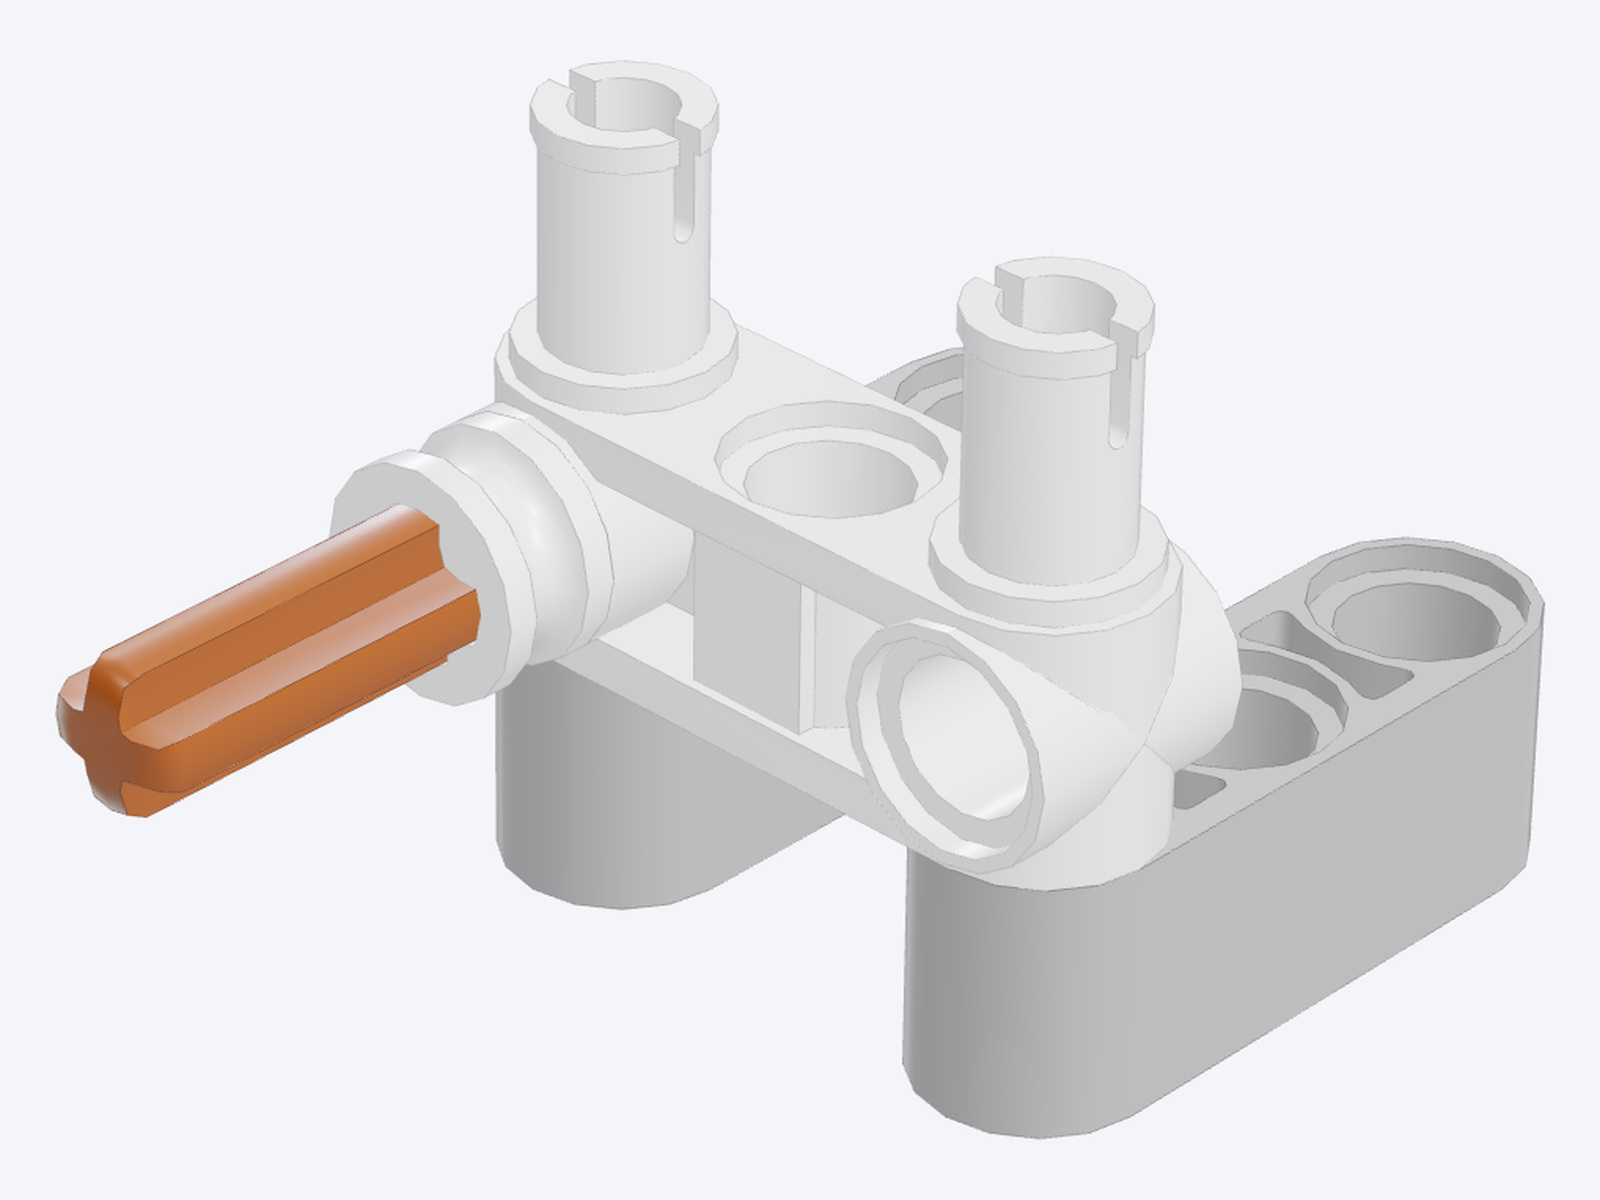
\includegraphics[width=.32\linewidth]{figures-v2/sequence-2.jpg}

\includegraphics[width=.32\linewidth]{figures-v2/sequence-3.jpg}\\
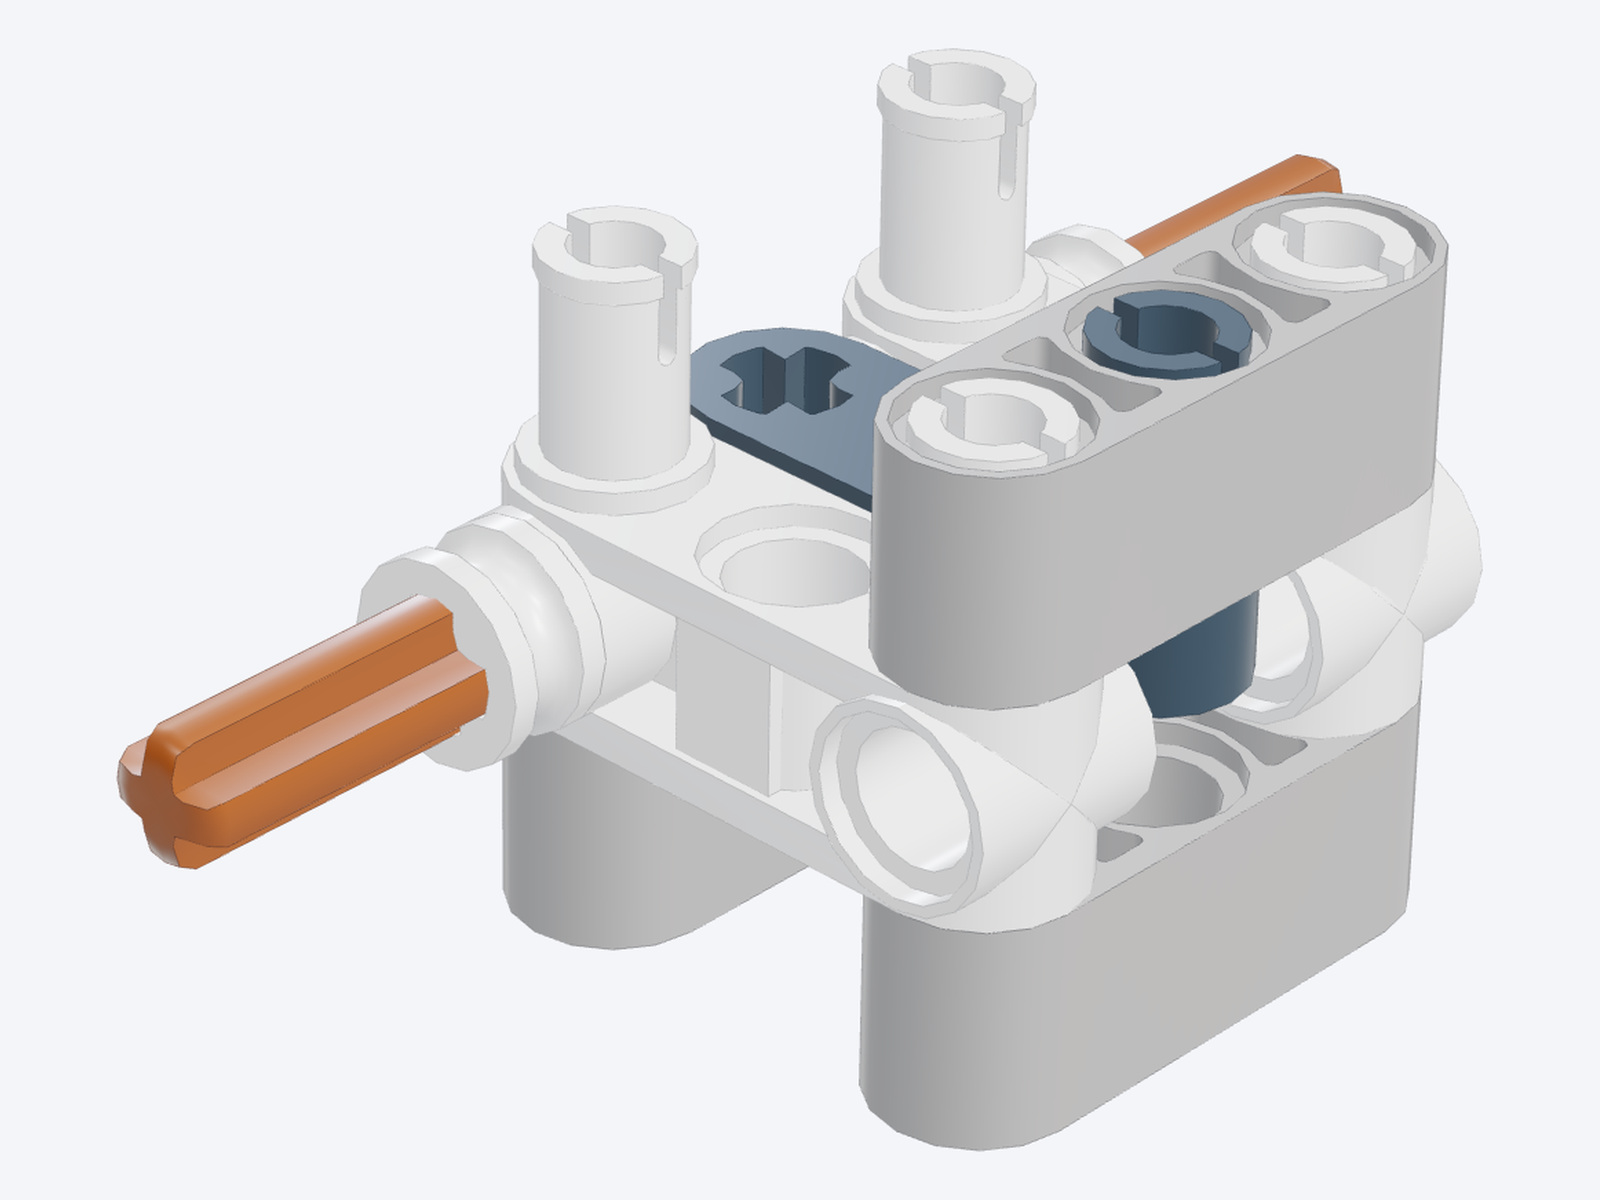
\includegraphics[width=.32\linewidth]{figures-v2/sequence-4.jpg}
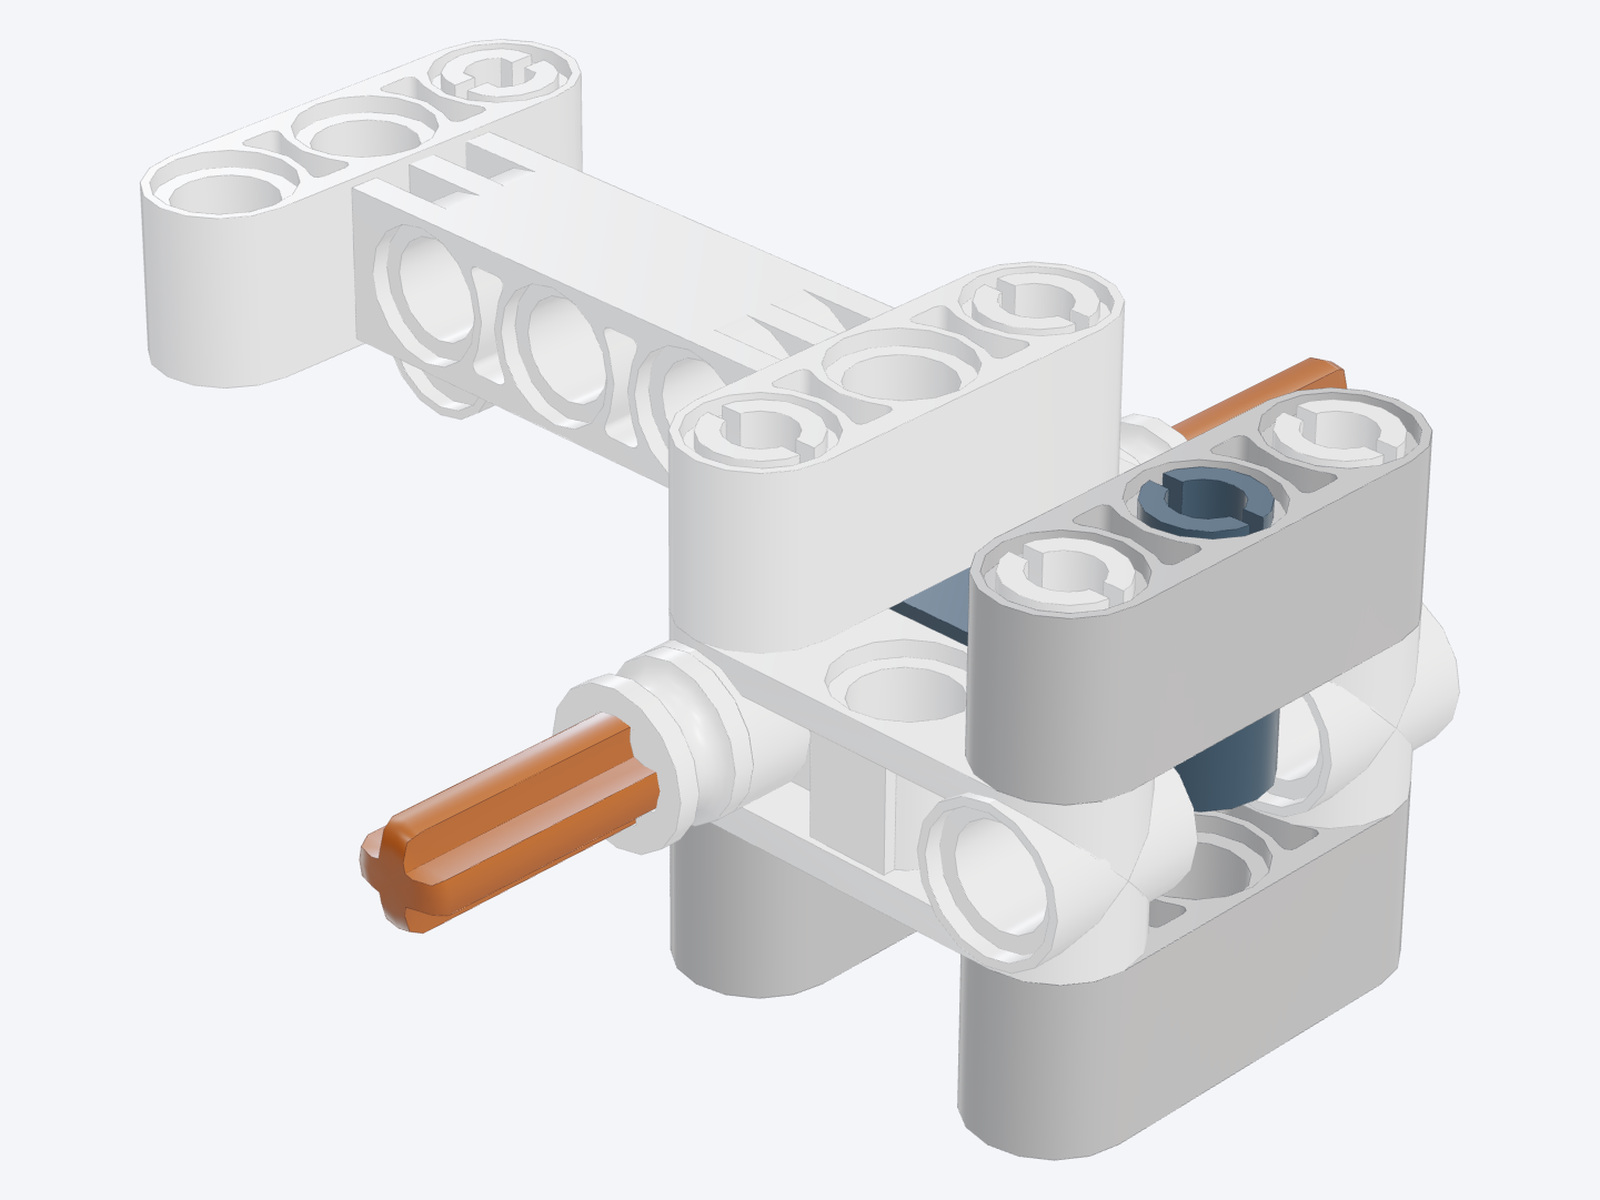
\includegraphics[width=.32\linewidth]{figures-v2/sequence-5.jpg}

\includegraphics[width=.32\linewidth]{figures-v2/sequence-6.jpg}
\end{center}
Step 1 requires start, later steps require the previous done fact;
each action forbids its own done fact, adds that fact, and costs one.
The budget is six and the goal is done-6. The displayed source window
is internal execution state; the model receives public facts/actions,
not the full source scene.

The following restoration frames show B0094 hidden, restored, and
still hidden after an unknown action is rejected. Visible counts are
128, 129 and 128. The target is restored at its original pose.
\begin{center}

\includegraphics[width=.32\linewidth]{figures-v2/restore-before.jpg}

\includegraphics[width=.32\linewidth]{figures-v2/restore-after.jpg}

\includegraphics[width=.32\linewidth]{figures-v2/restore-invalid.jpg}
\end{center}
Only accepted transitions alter facts or visibility. The action must
have its missing-target precondition, preserve the distractor's
presence and reach the present-target goal within unit budget.
No insertion trajectory, load capacity or contact force is measured.

\clearpage\section{Executable Evaluation Plan}
The sole model runner accepts only versioned public-input paths,
serializes a strict whitelist and saves actual wire bodies before
optional inference. It records exact adapter and code hashes,
checkpoint/API revision, fixed prompt, temperature, token limit,
image dimensions, timeout, raw response, usage and latency.
Moving aliases require a real frozen revision. Provider availability
has not been tested; offline adapter checks do not establish it.
\begin{center}\small\begin{tabularx}{\linewidth}{XXX}
\toprule
Config & Exact model ID & Revision\\\midrule
Claude & claude-sonnet-4-20250514 & 2025-05-14\\
Gemini & gemini-2.5-pro & Freeze before live use\\
GPT-4.1 & gpt-4.1-2025-04-14 & 2025-04-14\\
Llama 4 Scout & meta-llama/Llama-4-Scout-17B-16E-Instruct & Freeze before live use\\
Qwen3-VL & Qwen/Qwen3-VL-8B-Instruct & Freeze before live use\\
SmolVLM & HuggingFaceTB/SmolVLM-256M-Instruct & Freeze before live use\\
\bottomrule
\end{tabularx}
\end{center}
\subsection{Conditions and Paired Estimands}
\begin{center}\small\begin{tabularx}{\linewidth}{Xrr}
\toprule
Condition & $N$ & Exact success\\\midrule
standard & 617 & \\
text-without-image & 140 & \\
graph-edges-withheld & 146 & \\
full-scene & 140 & \\
background-mask & 140 & \\
operand-only & 140 & \\
choice-order & 469 & \\
edge-order & 146 & \\
id-permutation & 576 & \\
wrong-image & 140 & \\
camera-perturbation & 140 & \\
color-nuisance & 67 & \\
multi-view & 140 & \\
graph-intervention & 146 & \\
\bottomrule
\end{tabularx}
\end{center}
The full/mask pair keeps camera, lighting, scale and labels identical.
The crop changes both background and magnification. Standard images
were already operand-isolated in v1. Wrong-image controls preserve
operand labels and change semantic evidence. Color nuisance is confined
to type matching. Two-view access is fixed, not an adaptive interaction
agent. ID permutations are inverted for output scoring.

The 146 edge conditions exclude interface records, which contain no
edge list. Graph interventions change the answer under independent
recomputation; edge-order permutations preserve the graph. The
interventions describe hypothetical input evidence, not source repairs.
\begin{center}\small\begin{tabularx}{\linewidth}{XXrrr}
\toprule
A & B & $N$ & $\Delta$ macro & $\Delta$ micro\\\midrule
standard & text-without-image & 140 &  & \\
operand-only & wrong-image & 140 &  & \\
full-scene & background-mask & 140 &  & \\
full-scene & operand-only & 140 &  & \\
full-scene & text-without-image & 140 &  & \\
standard & graph-edges-withheld & 146 &  & \\
standard & graph-intervention & 146 &  & \\
operand-only & id-permutation & 140 &  & \\
standard & id-permutation & 436 &  & \\
standard & choice-order & 469 &  & \\
standard & edge-order & 146 &  & \\
operand-only & camera-perturbation & 140 &  & \\
operand-only & color-nuisance & 67 &  & \\
operand-only & multi-view & 140 &  & \\
\bottomrule
\end{tabularx}
\end{center}

Report each comparison by family, retaining complete paired task lists.
Source macro first averages eligible items per source, then sources;
micro averages items. A-minus-B paired differences use 10,000
source-cluster bootstrap draws, seed 20260918, and percentile 95\%
intervals, plus correct-to-wrong and wrong-to-correct counts.
An interval including zero means no stable gain detected, not proof
of equivalence. No equivalence margin is supplied.

All malformed, missing, refused or timed-out outputs remain failures.
There is one attempt per item with no hidden retries or output repair.
Unknown cost remains null. Source-linked views and items must remain
together in any future training split. There is currently no training
dataset or finalized train/test split.

\clearpage\section{Prospective Result Tables}
Every score cell in this section is intentionally blank. Counts are
measured eligibility, and model names are candidate configurations.
\subsection{Model comparison}
\begin{center}\small\input{tables-v2/plan-models.tex}\end{center}
\subsection{Family comparison}
\begin{center}\small\input{tables-v2/plan-families.tex}\end{center}
\subsection{Source-size bands}
\begin{center}\small\input{tables-v2/plan-scale.tex}\end{center}
\subsection{Actions}
\begin{center}\small\begin{tabularx}{\linewidth}{Xrrrr}
\toprule
Candidate family & Valid \% & Goal \% & Cost & Steps\\\midrule
SmolVLM &  &  &  & \\
Qwen3-VL &  &  &  & \\
Llama 4 &  &  &  & \\
GPT-4.1 &  &  &  & \\
Gemini &  &  &  & \\
Claude &  &  &  & \\
\bottomrule
\end{tabularx}
\end{center}
Goal success requires legal full execution; format validity alone
does not. Neither statistic demonstrates mechanical planning.
\clearpage\subsection{Information ablations}
\begin{center}\small\begin{tabularx}{\linewidth}{XXrrr}
\toprule
Condition & N & Acc. & Valid & Calls\\\midrule
Frozen operand-isolation image / structured public input & 617 &  &  & \\
Question and options without image & 140 &  &  & \\
Edge list withheld (interface records excluded) & 146 &  &  & \\
Full original assembly with operand labels & 140 &  &  & \\
Only operands visible; same full-scene camera & 140 &  &  & \\
Only operands visible; camera refitted to operands & 140 &  &  & \\
Semantically mismatched image with the same operand labels & 140 &  &  & \\
Two fixed views (not adaptive tool interaction) & 140 &  &  & \\
\bottomrule
\end{tabularx}
\end{center}
\subsection{Robustness}
\begin{center}\small\begin{tabularx}{\linewidth}{XXrrr}
\toprule
Perturbation & Eligible & Base & Changed & Consist.\\\midrule
Reverse option presentation; retain anonymous option IDs & 469 &  &  & \\
Reverse equivalent edge serialization & 146 &  &  & \\
Bijective B-number renaming in text and pixels & 576 &  &  & \\
Fixed alternative camera with original operand identities & 140 &  &  & \\
Desaturated operand image; type only & 67 &  &  & \\
One logical edge removal/addition changes the answer & 146 &  &  & \\
\bottomrule
\end{tabularx}
\end{center}
Mapped-output consistency may include two wrong answers and must be
reported with correct paired agreement.
\subsection{Resource use}
\begin{center}\small\begin{tabularx}{\linewidth}{Xrrrrr}
\toprule
Candidate family & Tokens & Calls & p50 s & p95 s & USD\\\midrule
SmolVLM &  &  &  &  & \\
Qwen3-VL &  &  &  &  & \\
Llama 4 &  &  &  &  & \\
GPT-4.1 &  &  &  &  & \\
Gemini &  &  &  &  & \\
Claude &  &  &  &  & \\
\bottomrule
\end{tabularx}
\end{center}
Calls include failures. Tokens and actual billed costs require real
receipts; local hardware costs need a separately declared convention.

\clearpage\section{Human Review and Physical Evidence}
All 140 visual questions require independent inspection of label
readability, color distinction and near-identical type alternatives.
The required task queue also contains 111 nonvisual flagged items.
The 573 source-local intersection pairs have separate stable IDs.
They are candidates without recognized mating interfaces, not certified
collision defects. Intended mating, approximate meshes, source errors
and unresolved cases require distinct recorded decisions.
\begin{center}\small\input{tables-v2/plan-human.tex}\end{center}
\begin{center}\small\begin{tabularx}{\linewidth}{Xrrrr}
\toprule
Validation procedure & Reviewed & Pass & Fail & Unresolved\\\midrule
Connector-aware pair inspection &  &  &  & \\
Unsupported-part adjudication &  &  &  & \\
Insertion / extraction study &  &  &  & \\
Gravity / friction simulation &  &  &  & \\
Physical assembly validation &  &  &  & \\
\bottomrule
\end{tabularx}
\end{center}
The review UI binds each decision to release version, source SHA256,
task or pair content hash, operands, reviewer, reason and timestamp.
Import rejects unknown or stale units; independent reviewers retain
separate records and disagreements. Software fixtures use temporary
storage and never create production human approvals.
Reviewing an intersection is not a gravity or force experiment.

Diagnostic localization additionally requires controlled target
failures, non-target-module stability and restoration experiments.
Separate family scores, score products and regressions cannot replace
that evidence. The optional cross-module extension was not implemented.

\section{Reproduction and Measurement Repair}
The v1 freeze covers 2,131 files. V2 uses independent namespaces for
code, inputs, internal scoring data, figures and manuscripts.
Graph deletion now uses integer outputs because 63/73 correct answers
lie at the legal maximum. Legal four-choice balancing cannot remove
that extremum cue while preserving all answers.
Author-step semantic ranks are balanced at 14/14/14/13.
Ordered references are absent from all model requests; internal
type-match positions are 14/13/13/13/14. Interface always has five
options. Redundant missing-instance metadata is removed.

All 617 independent oracle checks, 75 public-action solves and 5,154
negative controls pass. All 907 new images reproduce byte for byte.
These are software checks, not human or model scores. Semantic
majorities, fixed responses and operand reuse remain explicit.
The publication generator derives all tables from current JSON and
hashes its inputs/outputs. Build and verification commands are in
\path{BUILD-v2.md}. The standalone v2 review page is
\path{ldraw-v2.html}; it does not replace the protected v1 route.

\clearpage\section{31028: Sea Plane}
53 source instances; 15 tasks; D1 size band. 27 type strings; 10 color codes; 0 unsupported instances; 0 intersection candidates. 0 expanded author steps. Independent reparse: passed.
\begin{center}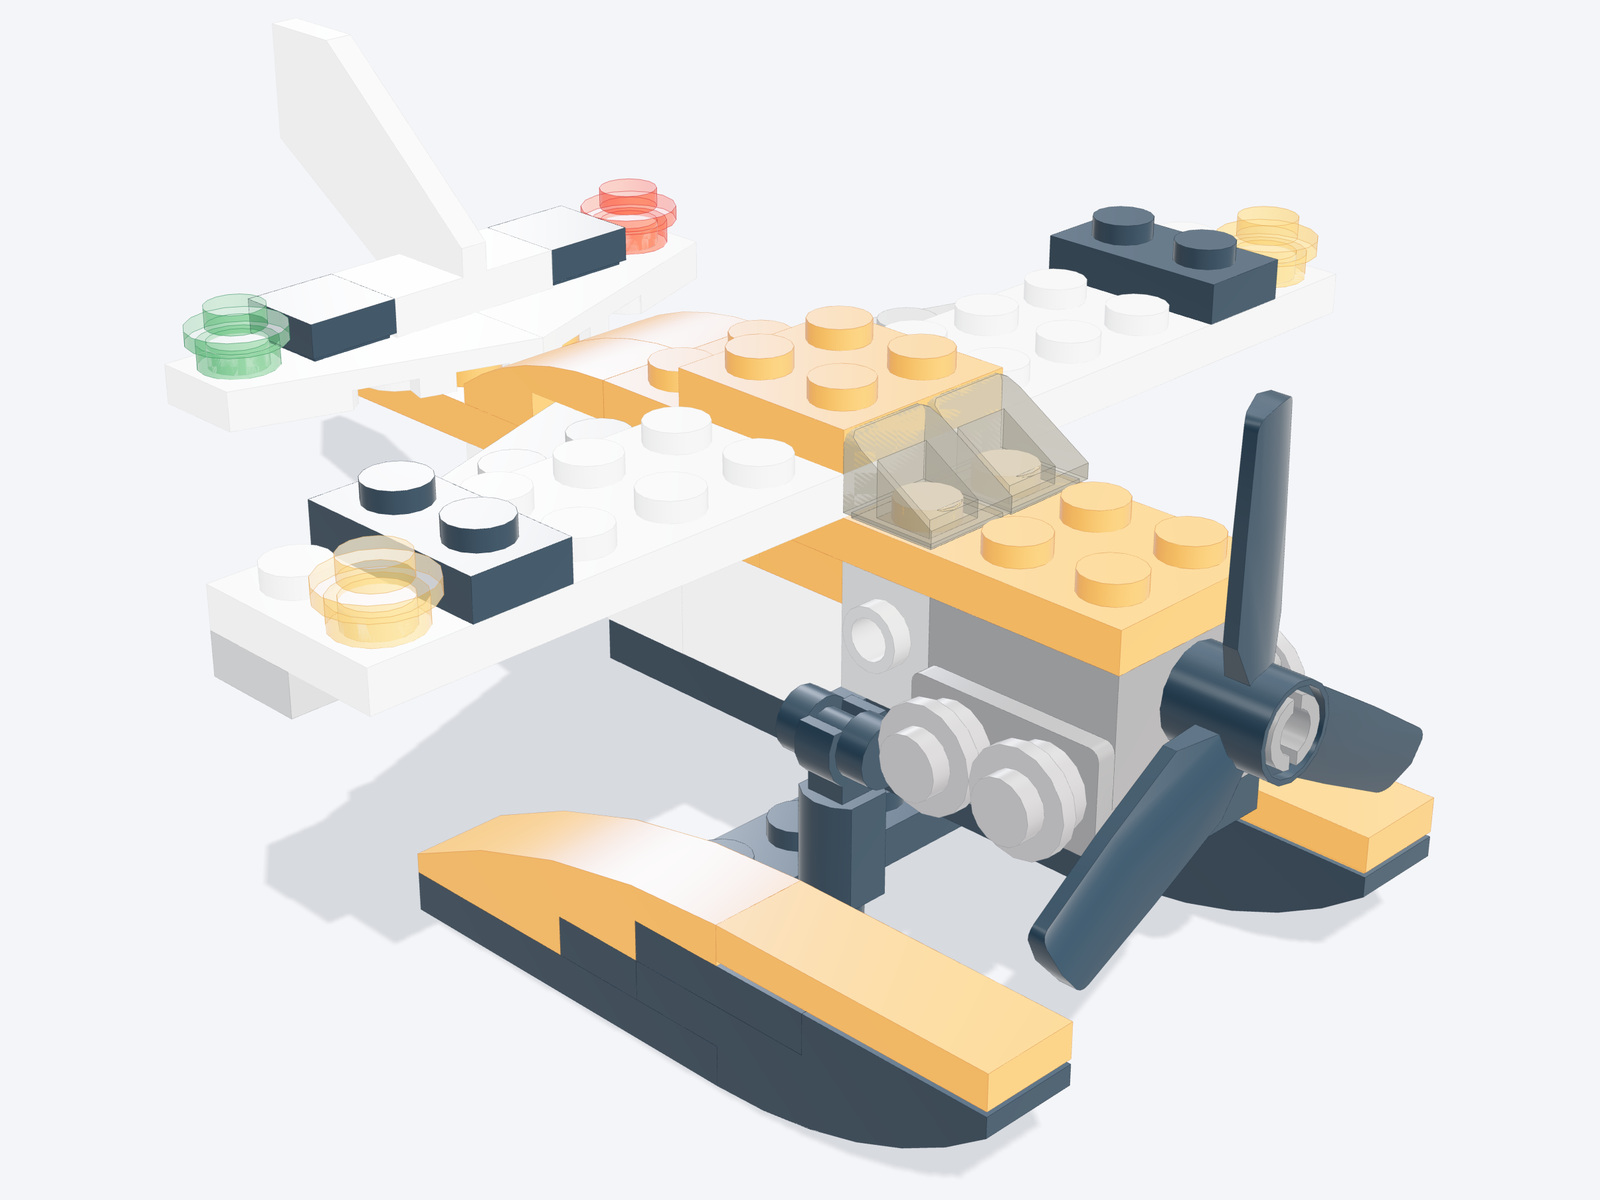
\includegraphics[width=.65\linewidth]{figures-v2/31028-iso.jpg}\end{center}
\paragraph{Attribution.}Merlijn Wissink [legolijntje]. CC BY 2.0.\par\url{https://library.ldraw.org/omr/sets/259}
\paragraph{Source SHA256.}\path{d2619a85e973430a1b256d607fe8e44a865beb05ef63ac8028a5109c228ee97c}
\paragraph{Connector records.}stud: 108; axle: 5; hinge: 0; fixed: 0; ball: 0
\paragraph{Public input lock.}\path{f5df0685f7d89d74435eef34a311b18fc9d14ce4bc39a3ab7bbf43c78b3eb9ba}
\paragraph{Status.}Source preservation does not certify stability. Reference outputs below are internal review material. Full model inputs are the versioned public JSON and numbered PNGs.
\begin{enumerate}
\item \textbf{ld2-31028-color-1}. Identify the original color of B0018; numbered isolation is allowed.
\par{\small color; visual; atomic; single-choice.\par\textit{Operands:} B0018 = brick\_000018\par\textit{Public evidence summary:} Numbered PNG: benchmark/ldraw-v2/inputs/views/ld2-31028-color-1.png; structured input = \{\}.\par\textit{Options:} A: Black; B: Orange; C: Light Bluish Grey; D: Trans Brown\par\textit{Reference output:} \{"choiceId": "B"\}\par\textit{Derivation:} source colorName by rendered B-label; source oracle only\par\textit{Equivalence:} exact declared response\par\textit{Review:} pending required human review.}
\item \textbf{ld2-31028-shape-match-1}. Ignoring color and pose, which numbered instance has the same LDraw part type as B0018?
\par{\small shape-match; visual; atomic; single-choice.\par\textit{Operands:} B0008 = brick\_000008, B0018 = brick\_000018, B0031 = brick\_000031, B0042 = brick\_000042, B0004 = brick\_000004\par\textit{Public evidence summary:} Numbered PNG: benchmark/ldraw-v2/inputs/views/ld2-31028-shape-match-1.png; structured input = \{\}.\par\textit{Options:} A: B0008; B: B0031; C: B0004; D: B0042\par\textit{Reference output:} \{"choiceId": "B"\}\par\textit{Derivation:} source partNumber equality across labeled candidates; source oracle only\par\textit{Equivalence:} same source partNumber; ignore color and pose; perceptual equivalence pending\par\textit{Review:} pending required human review.}
\item \textbf{ld2-31028-distance-1}. Using the supplied geometry bounding-box centers, which candidate is nearest to B0018?
\par{\small distance; source-data; atomic; single-choice.\par\textit{Operands:} B0024 = brick\_000024, B0018 = brick\_000018, B0028 = brick\_000028, B0043 = brick\_000043\par\textit{Public evidence summary:} \{"coordinateFrame": "Viewer world, millimeters, Euclidean distance", "centers": \{"B0018": [0, 8.8, -36], "B0028": [0, 15.2, -24], "B0043": [-17.2, -12, 0], "B0024": [-20, 15.2, -56]\}\}\par\textit{Options:} A: B0043; B: B0024; C: B0028\par\textit{Reference output:} \{"choiceId": "C"\}\par\textit{Derivation:} Euclidean norm from public rounded centers\par\textit{Equivalence:} exact declared response\par\textit{Review:} machine checks passed; no human certification.}
\item \textbf{ld2-31028-color-2}. Identify the original color of B0035; numbered isolation is allowed.
\par{\small color; visual; atomic; single-choice.\par\textit{Operands:} B0035 = brick\_000035\par\textit{Public evidence summary:} Numbered PNG: benchmark/ldraw-v2/inputs/views/ld2-31028-color-2.png; structured input = \{\}.\par\textit{Options:} A: Trans Orange; B: Black; C: Trans Brown; D: White\par\textit{Reference output:} \{"choiceId": "C"\}\par\textit{Derivation:} source colorName by rendered B-label; source oracle only\par\textit{Equivalence:} exact declared response\par\textit{Review:} pending required human review.}
\item \textbf{ld2-31028-shape-match-2}. Ignoring color and pose, which numbered instance has the same LDraw part type as B0035?
\par{\small shape-match; visual; atomic; single-choice.\par\textit{Operands:} B0034 = brick\_000034, B0038 = brick\_000038, B0045 = brick\_000045, B0035 = brick\_000035, B0012 = brick\_000012\par\textit{Public evidence summary:} Numbered PNG: benchmark/ldraw-v2/inputs/views/ld2-31028-shape-match-2.png; structured input = \{\}.\par\textit{Options:} A: B0034; B: B0045; C: B0038; D: B0012\par\textit{Reference output:} \{"choiceId": "A"\}\par\textit{Derivation:} source partNumber equality across labeled candidates; source oracle only\par\textit{Equivalence:} same source partNumber; ignore color and pose; perceptual equivalence pending\par\textit{Review:} pending required human review.}
\item \textbf{ld2-31028-distance-2}. Using the supplied geometry bounding-box centers, which candidate is nearest to B0035?
\par{\small distance; source-data; atomic; single-choice.\par\textit{Operands:} B0035 = brick\_000035, B0027 = brick\_000027, B0006 = brick\_000006, B0014 = brick\_000014\par\textit{Public evidence summary:} \{"coordinateFrame": "Viewer world, millimeters, Euclidean distance", "centers": \{"B0035": [4, 15.92, 0], "B0014": [-12, 0.8, 8], "B0006": [0, -0.8, 0], "B0027": [-24, 12, -23.8]\}\}\par\textit{Options:} A: B0027; B: B0006; C: B0014\par\textit{Reference output:} \{"choiceId": "B"\}\par\textit{Derivation:} Euclidean norm from public rounded centers\par\textit{Equivalence:} exact declared response\par\textit{Review:} machine checks passed; no human certification.}
\item \textbf{ld2-31028-interface-1}. Classify the supplied connector record for B0053 and B0006. This does not certify load capacity.
\par{\small interface; connector-graph; metacognitive; single-choice.\par\textit{Operands:} B0053 = brick\_000053, B0006 = brick\_000006\par\textit{Public evidence summary:} \{"connectorRecord": \{"family": "axle", "aConnector": 0, "bConnector": 1\}, "scope": "Upstream connector tolerances and inset mesh intersections; unknown parts remain explicit, separate scene objects are not glued together; no load/force validation."\}\par\textit{Options:} A: fixed; B: hinge; C: stud; D: axle; E: ball\par\textit{Reference output:} \{"choiceId": "D"\}\par\textit{Derivation:} public connectorRecord.family equality\par\textit{Equivalence:} exact declared response\par\textit{Review:} machine checks passed; no human certification.}
\item \textbf{ld2-31028-interface-2}. Classify the supplied connector record for B0042 and B0044. This does not certify load capacity.
\par{\small interface; connector-graph; metacognitive; single-choice.\par\textit{Operands:} B0044 = brick\_000044, B0042 = brick\_000042\par\textit{Public evidence summary:} \{"connectorRecord": \{"family": "stud", "aConnector": 11, "bConnector": 10\}, "scope": "Upstream connector tolerances and inset mesh intersections; unknown parts remain explicit, separate scene objects are not glued together; no load/force validation."\}\par\textit{Options:} A: fixed; B: ball; C: stud; D: hinge; E: axle\par\textit{Reference output:} \{"choiceId": "C"\}\par\textit{Derivation:} public connectorRecord.family equality\par\textit{Equivalence:} exact declared response\par\textit{Review:} machine checks passed; no human certification.}
\item \textbf{ld2-31028-neighbors-1}. Select every candidate directly adjacent to B0027 in the supplied connector graph.
\par{\small neighbors; connector-graph; metacognitive; multiple-choice.\par\textit{Operands:} B0038 = brick\_000038, B0018 = brick\_000018, B0031 = brick\_000031, B0027 = brick\_000027, B0047 = brick\_000047, B0028 = brick\_000028\par\textit{Public evidence summary:} 4 unique undirected pairs\par\textit{Options:} A: B0028; B: B0031; C: B0038; D: B0018; E: B0047\par\textit{Reference output:} \{"choiceIds": ["A", "B", "D"]\}\par\textit{Derivation:} public incident edge endpoint set\par\textit{Equivalence:} unordered exact set; duplicate IDs invalid\par\textit{Review:} machine checks passed; no human certification.}
\item \textbf{ld2-31028-graph-removal-1}. Delete B0027 and its incident edges from this local graph. How many connected components remain? Do not infer physical extractability.
\par{\small graph-removal; connector-graph; graph-internal; integer.\par\textit{Operands:} B0031 = brick\_000031, B0027 = brick\_000027, B0028 = brick\_000028, B0047 = brick\_000047, B0018 = brick\_000018, B0038 = brick\_000038\par\textit{Public evidence summary:} 4 unique undirected pairs; 6 nodes\par\textit{Reference output:} \{"value": 4\}\par\textit{Derivation:} union-find component count after public target deletion\par\textit{Equivalence:} exact declared response\par\textit{Review:} machine checks passed; no human certification.}
\item \textbf{ld2-31028-neighbors-2}. Select every candidate directly adjacent to B0047 in the supplied connector graph.
\par{\small neighbors; connector-graph; metacognitive; multiple-choice.\par\textit{Operands:} B0044 = brick\_000044, B0049 = brick\_000049, B0050 = brick\_000050, B0001 = brick\_000001, B0048 = brick\_000048, B0047 = brick\_000047\par\textit{Public evidence summary:} 5 unique undirected pairs\par\textit{Options:} A: B0050; B: B0044; C: B0049; D: B0001; E: B0048\par\textit{Reference output:} \{"choiceIds": ["A", "C", "E"]\}\par\textit{Derivation:} public incident edge endpoint set\par\textit{Equivalence:} unordered exact set; duplicate IDs invalid\par\textit{Review:} machine checks passed; no human certification.}
\item \textbf{ld2-31028-graph-removal-2}. Delete B0047 and its incident edges from this local graph. How many connected components remain? Do not infer physical extractability.
\par{\small graph-removal; connector-graph; graph-internal; integer.\par\textit{Operands:} B0048 = brick\_000048, B0044 = brick\_000044, B0050 = brick\_000050, B0049 = brick\_000049, B0047 = brick\_000047, B0001 = brick\_000001\par\textit{Public evidence summary:} 5 unique undirected pairs; 6 nodes\par\textit{Reference output:} \{"value": 3\}\par\textit{Derivation:} union-find component count after public target deletion\par\textit{Equivalence:} exact declared response\par\textit{Review:} machine checks passed; no human certification.}
\item \textbf{ld2-31028-evidence-limit-1}. Only source geometry, connector matching and mesh intersection audits are available. Without mass, friction, material or dynamic tests, is gravitational stability established?
\par{\small evidence-limit; source-data; metacognitive; single-choice.\par\textit{Operands:} none\par\textit{Public evidence summary:} \{"available": ["Original CAD", "Connector inference", "Inset-mesh intersection candidates"]\}\par\textit{Options:} A: Not established by this evidence; B: Established\par\textit{Reference output:} \{"choiceId": "A"\}\par\textit{Derivation:} fixed epistemic control label\par\textit{Equivalence:} exact declared response\par\textit{Review:} machine checks passed; no human certification.}
\item \textbf{ld2-31028-restore-instance-1}. The display copy hides B0018. Restore only that numbered instance, preserving all other instances and source poses.
\par{\small restore-instance; scene-edit; procedural; actions.\par\textit{Operands:} B0018 = brick\_000018, B0001 = brick\_000001\par\textit{Public evidence summary:} 2 public actions; budget 1; \{"initialFacts": ["missing-brick\_000018", "present-brick\_000001"], "goalFacts": ["present-brick\_000018", "present-brick\_000001"], "absentFacts": ["missing-brick\_000018"]\}\par\textit{Reference output:} \{"actionIds": ["restore-B0018"]\}\par\textit{Derivation:} public precondition solver\par\textit{Equivalence:} any legal sequence reaching all goals within budget; display-only semantics\par\textit{Review:} machine checks passed; no human certification.}
\item \textbf{ld2-31028-restore-instance-2}. The display copy hides B0035. Restore only that numbered instance, preserving all other instances and source poses.
\par{\small restore-instance; scene-edit; procedural; actions.\par\textit{Operands:} B0001 = brick\_000001, B0035 = brick\_000035\par\textit{Public evidence summary:} 2 public actions; budget 1; \{"initialFacts": ["missing-brick\_000035", "present-brick\_000001"], "goalFacts": ["present-brick\_000035", "present-brick\_000001"], "absentFacts": ["missing-brick\_000035"]\}\par\textit{Reference output:} \{"actionIds": ["restore-B0035"]\}\par\textit{Derivation:} public precondition solver\par\textit{Equivalence:} any legal sequence reaching all goals within budget; display-only semantics\par\textit{Review:} machine checks passed; no human certification.}
\end{enumerate}
\clearpage\section{31027: Blue Racer}
67 source instances; 17 tasks; D1 size band. 24 type strings; 10 color codes; 0 unsupported instances; 0 intersection candidates. 0 expanded author steps. Independent reparse: passed.
\begin{center}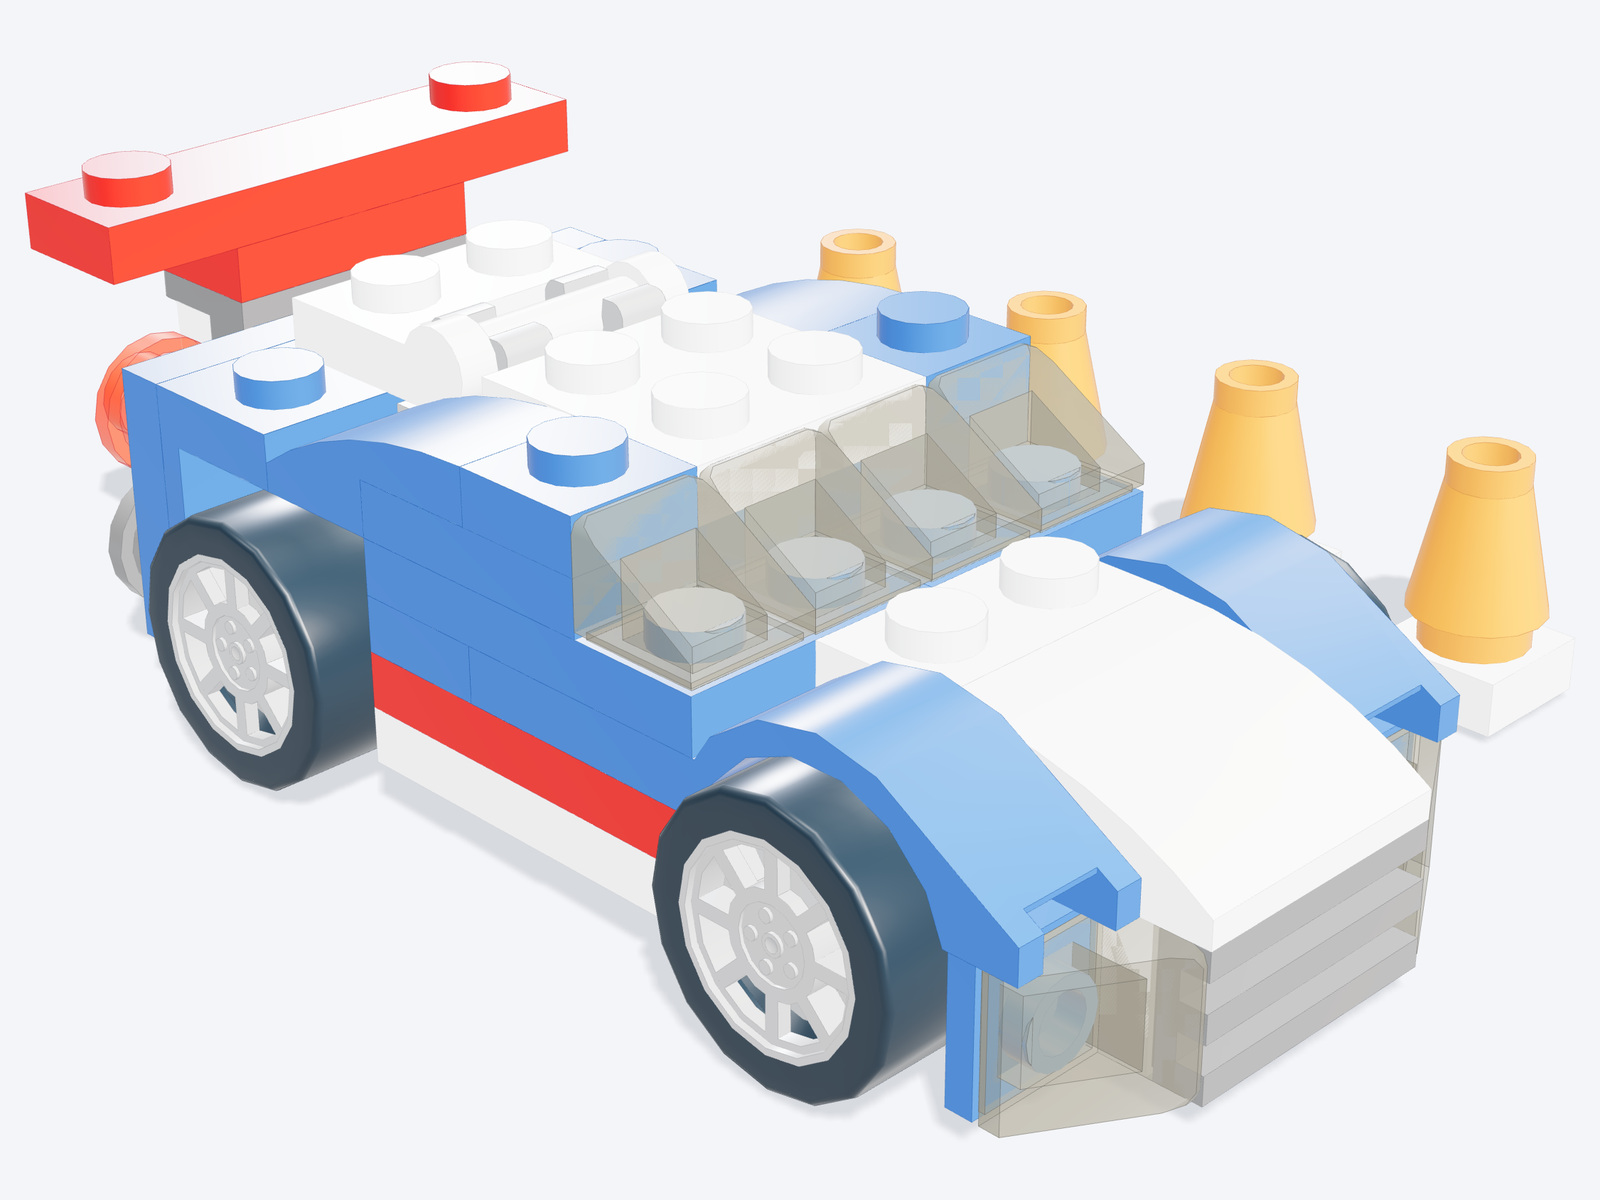
\includegraphics[width=.65\linewidth]{figures-v2/31027-iso.jpg}\end{center}
\paragraph{Attribution.}Merlijn Wissink [legolijntje]. CC BY 2.0.\par\url{https://library.ldraw.org/omr/sets/223}
\paragraph{Source SHA256.}\path{1f1975602ce9a63f2954c8da97f4fc13a473f709afa4a25b1022add33b55cfd1}
\paragraph{Connector records.}stud: 112; axle: 6; hinge: 4; fixed: 16; ball: 0
\paragraph{Public input lock.}\path{8a8536853ab343c715c653f7f072a11d937291636d5fa3e2be647c8405c190bc}
\paragraph{Status.}Source preservation does not certify stability. Reference outputs below are internal review material. Full model inputs are the versioned public JSON and numbered PNGs.
\begin{enumerate}
\item \textbf{ld2-31027-color-1}. Identify the original color of B0045; numbered isolation is allowed.
\par{\small color; visual; atomic; single-choice.\par\textit{Operands:} B0045 = brick\_000045\par\textit{Public evidence summary:} Numbered PNG: benchmark/ldraw-v2/inputs/views/ld2-31027-color-1.png; structured input = \{\}.\par\textit{Options:} A: Trans Brown; B: Trans Red; C: Orange; D: Light Bluish Grey\par\textit{Reference output:} \{"choiceId": "A"\}\par\textit{Derivation:} source colorName by rendered B-label; source oracle only\par\textit{Equivalence:} exact declared response\par\textit{Review:} pending required human review.}
\item \textbf{ld2-31027-shape-match-1}. Ignoring color and pose, which numbered instance has the same LDraw part type as B0045?
\par{\small shape-match; visual; atomic; single-choice.\par\textit{Operands:} B0045 = brick\_000045, B0054 = brick\_000054, B0019 = brick\_000019, B0036 = brick\_000036, B0062 = brick\_000062\par\textit{Public evidence summary:} Numbered PNG: benchmark/ldraw-v2/inputs/views/ld2-31027-shape-match-1.png; structured input = \{\}.\par\textit{Options:} A: B0062; B: B0019; C: B0036; D: B0054\par\textit{Reference output:} \{"choiceId": "B"\}\par\textit{Derivation:} source partNumber equality across labeled candidates; source oracle only\par\textit{Equivalence:} same source partNumber; ignore color and pose; perceptual equivalence pending\par\textit{Review:} pending required human review.}
\item \textbf{ld2-31027-distance-1}. Using the supplied geometry bounding-box centers, which candidate is nearest to B0045?
\par{\small distance; source-data; atomic; single-choice.\par\textit{Operands:} B0036 = brick\_000036, B0045 = brick\_000045, B0051 = brick\_000051, B0040 = brick\_000040\par\textit{Public evidence summary:} \{"coordinateFrame": "Viewer world, millimeters, Euclidean distance", "centers": \{"B0045": [12, 9.52, 12], "B0040": [12, 9.600012, -8], "B0051": [12, -2.4, -31.2], "B0036": [8, 8.8, 0]\}\}\par\textit{Options:} A: B0051; B: B0040; C: B0036\par\textit{Reference output:} \{"choiceId": "C"\}\par\textit{Derivation:} Euclidean norm from public rounded centers\par\textit{Equivalence:} exact declared response\par\textit{Review:} machine checks passed; no human certification.}
\item \textbf{ld2-31027-color-2}. Identify the original color of B0050; numbered isolation is allowed.
\par{\small color; visual; atomic; single-choice.\par\textit{Operands:} B0050 = brick\_000050\par\textit{Public evidence summary:} Numbered PNG: benchmark/ldraw-v2/inputs/views/ld2-31027-color-2.png; structured input = \{\}.\par\textit{Options:} A: Black; B: Red; C: White; D: Light Bluish Grey\par\textit{Reference output:} \{"choiceId": "C"\}\par\textit{Derivation:} source colorName by rendered B-label; source oracle only\par\textit{Equivalence:} exact declared response\par\textit{Review:} pending required human review.}
\item \textbf{ld2-31027-shape-match-2}. Ignoring color and pose, which numbered instance has the same LDraw part type as B0050?
\par{\small shape-match; visual; atomic; single-choice.\par\textit{Operands:} B0002 = brick\_000002, B0034 = brick\_000034, B0050 = brick\_000050, B0014 = brick\_000014, B0043 = brick\_000043\par\textit{Public evidence summary:} Numbered PNG: benchmark/ldraw-v2/inputs/views/ld2-31027-shape-match-2.png; structured input = \{\}.\par\textit{Options:} A: B0014; B: B0002; C: B0043; D: B0034\par\textit{Reference output:} \{"choiceId": "D"\}\par\textit{Derivation:} source partNumber equality across labeled candidates; source oracle only\par\textit{Equivalence:} same source partNumber; ignore color and pose; perceptual equivalence pending\par\textit{Review:} pending required human review.}
\item \textbf{ld2-31027-distance-2}. Using the supplied geometry bounding-box centers, which candidate is nearest to B0050?
\par{\small distance; source-data; atomic; single-choice.\par\textit{Operands:} B0058 = brick\_000058, B0046 = brick\_000046, B0050 = brick\_000050, B0019 = brick\_000019\par\textit{Public evidence summary:} \{"coordinateFrame": "Viewer world, millimeters, Euclidean distance", "centers": \{"B0050": [0, 1.6, -32.000012], "B0019": [-12, -4, 36.72], "B0046": [-12, 12, 4], "B0058": [-8, 2.4, -21.6]\}\}\par\textit{Options:} A: B0046; B: B0058; C: B0019\par\textit{Reference output:} \{"choiceId": "B"\}\par\textit{Derivation:} Euclidean norm from public rounded centers\par\textit{Equivalence:} exact declared response\par\textit{Review:} machine checks passed; no human certification.}
\item \textbf{ld2-31027-interface-1}. Classify the supplied connector record for B0037 and B0059. This does not certify load capacity.
\par{\small interface; connector-graph; metacognitive; single-choice.\par\textit{Operands:} B0059 = brick\_000059, B0037 = brick\_000037\par\textit{Public evidence summary:} \{"connectorRecord": \{"family": "axle", "aConnector": 1, "bConnector": 0\}, "scope": "Upstream connector tolerances and inset mesh intersections; unknown parts remain explicit, separate scene objects are not glued together; no load/force validation."\}\par\textit{Options:} A: axle; B: fixed; C: stud; D: hinge; E: ball\par\textit{Reference output:} \{"choiceId": "A"\}\par\textit{Derivation:} public connectorRecord.family equality\par\textit{Equivalence:} exact declared response\par\textit{Review:} machine checks passed; no human certification.}
\item \textbf{ld2-31027-interface-2}. Classify the supplied connector record for B0026 and B0027. This does not certify load capacity.
\par{\small interface; connector-graph; metacognitive; single-choice.\par\textit{Operands:} B0027 = brick\_000027, B0026 = brick\_000026\par\textit{Public evidence summary:} \{"connectorRecord": \{"family": "fixed", "aConnector": 1, "bConnector": 1\}, "scope": "Upstream connector tolerances and inset mesh intersections; unknown parts remain explicit, separate scene objects are not glued together; no load/force validation."\}\par\textit{Options:} A: fixed; B: ball; C: stud; D: hinge; E: axle\par\textit{Reference output:} \{"choiceId": "A"\}\par\textit{Derivation:} public connectorRecord.family equality\par\textit{Equivalence:} exact declared response\par\textit{Review:} machine checks passed; no human certification.}
\item \textbf{ld2-31027-interface-3}. Classify the supplied connector record for B0002 and B0024. This does not certify load capacity.
\par{\small interface; connector-graph; metacognitive; single-choice.\par\textit{Operands:} B0002 = brick\_000002, B0024 = brick\_000024\par\textit{Public evidence summary:} \{"connectorRecord": \{"family": "hinge", "aConnector": 2, "bConnector": 3\}, "scope": "Upstream connector tolerances and inset mesh intersections; unknown parts remain explicit, separate scene objects are not glued together; no load/force validation."\}\par\textit{Options:} A: fixed; B: ball; C: stud; D: axle; E: hinge\par\textit{Reference output:} \{"choiceId": "E"\}\par\textit{Derivation:} public connectorRecord.family equality\par\textit{Equivalence:} exact declared response\par\textit{Review:} machine checks passed; no human certification.}
\item \textbf{ld2-31027-interface-4}. Classify the supplied connector record for B0060 and B0061. This does not certify load capacity.
\par{\small interface; connector-graph; metacognitive; single-choice.\par\textit{Operands:} B0060 = brick\_000060, B0061 = brick\_000061\par\textit{Public evidence summary:} \{"connectorRecord": \{"family": "stud", "aConnector": 1, "bConnector": 3\}, "scope": "Upstream connector tolerances and inset mesh intersections; unknown parts remain explicit, separate scene objects are not glued together; no load/force validation."\}\par\textit{Options:} A: fixed; B: hinge; C: ball; D: stud; E: axle\par\textit{Reference output:} \{"choiceId": "D"\}\par\textit{Derivation:} public connectorRecord.family equality\par\textit{Equivalence:} exact declared response\par\textit{Review:} machine checks passed; no human certification.}
\item \textbf{ld2-31027-neighbors-1}. Select every candidate directly adjacent to B0012 in the supplied connector graph.
\par{\small neighbors; connector-graph; metacognitive; multiple-choice.\par\textit{Operands:} B0001 = brick\_000001, B0012 = brick\_000012, B0031 = brick\_000031, B0059 = brick\_000059, B0055 = brick\_000055\par\textit{Public evidence summary:} 2 unique undirected pairs\par\textit{Options:} A: B0059; B: B0001; C: B0055; D: B0031\par\textit{Reference output:} \{"choiceIds": ["B", "D"]\}\par\textit{Derivation:} public incident edge endpoint set\par\textit{Equivalence:} unordered exact set; duplicate IDs invalid\par\textit{Review:} machine checks passed; no human certification.}
\item \textbf{ld2-31027-graph-removal-1}. Delete B0012 and its incident edges from this local graph. How many connected components remain? Do not infer physical extractability.
\par{\small graph-removal; connector-graph; graph-internal; integer.\par\textit{Operands:} B0012 = brick\_000012, B0059 = brick\_000059, B0055 = brick\_000055, B0031 = brick\_000031, B0001 = brick\_000001\par\textit{Public evidence summary:} 2 unique undirected pairs; 5 nodes\par\textit{Reference output:} \{"value": 4\}\par\textit{Derivation:} union-find component count after public target deletion\par\textit{Equivalence:} exact declared response\par\textit{Review:} machine checks passed; no human certification.}
\item \textbf{ld2-31027-neighbors-2}. Select every candidate directly adjacent to B0024 in the supplied connector graph.
\par{\small neighbors; connector-graph; metacognitive; multiple-choice.\par\textit{Operands:} B0053 = brick\_000053, B0024 = brick\_000024, B0025 = brick\_000025, B0002 = brick\_000002, B0058 = brick\_000058\par\textit{Public evidence summary:} 2 unique undirected pairs\par\textit{Options:} A: B0053; B: B0025; C: B0002; D: B0058\par\textit{Reference output:} \{"choiceIds": ["B", "C"]\}\par\textit{Derivation:} public incident edge endpoint set\par\textit{Equivalence:} unordered exact set; duplicate IDs invalid\par\textit{Review:} machine checks passed; no human certification.}
\item \textbf{ld2-31027-graph-removal-2}. Delete B0024 and its incident edges from this local graph. How many connected components remain? Do not infer physical extractability.
\par{\small graph-removal; connector-graph; graph-internal; integer.\par\textit{Operands:} B0024 = brick\_000024, B0058 = brick\_000058, B0053 = brick\_000053, B0002 = brick\_000002, B0025 = brick\_000025\par\textit{Public evidence summary:} 2 unique undirected pairs; 5 nodes\par\textit{Reference output:} \{"value": 4\}\par\textit{Derivation:} union-find component count after public target deletion\par\textit{Equivalence:} exact declared response\par\textit{Review:} machine checks passed; no human certification.}
\item \textbf{ld2-31027-evidence-limit-1}. Only source geometry, connector matching and mesh intersection audits are available. Without mass, friction, material or dynamic tests, is gravitational stability established?
\par{\small evidence-limit; source-data; metacognitive; single-choice.\par\textit{Operands:} none\par\textit{Public evidence summary:} \{"available": ["Original CAD", "Connector inference", "Inset-mesh intersection candidates"]\}\par\textit{Options:} A: Established; B: Not established by this evidence\par\textit{Reference output:} \{"choiceId": "B"\}\par\textit{Derivation:} fixed epistemic control label\par\textit{Equivalence:} exact declared response\par\textit{Review:} machine checks passed; no human certification.}
\item \textbf{ld2-31027-restore-instance-1}. The display copy hides B0045. Restore only that numbered instance, preserving all other instances and source poses.
\par{\small restore-instance; scene-edit; procedural; actions.\par\textit{Operands:} B0001 = brick\_000001, B0045 = brick\_000045\par\textit{Public evidence summary:} 2 public actions; budget 1; \{"initialFacts": ["missing-brick\_000045", "present-brick\_000001"], "goalFacts": ["present-brick\_000045", "present-brick\_000001"], "absentFacts": ["missing-brick\_000045"]\}\par\textit{Reference output:} \{"actionIds": ["restore-B0045"]\}\par\textit{Derivation:} public precondition solver\par\textit{Equivalence:} any legal sequence reaching all goals within budget; display-only semantics\par\textit{Review:} machine checks passed; no human certification.}
\item \textbf{ld2-31027-restore-instance-2}. The display copy hides B0050. Restore only that numbered instance, preserving all other instances and source poses.
\par{\small restore-instance; scene-edit; procedural; actions.\par\textit{Operands:} B0050 = brick\_000050, B0001 = brick\_000001\par\textit{Public evidence summary:} 2 public actions; budget 1; \{"initialFacts": ["missing-brick\_000050", "present-brick\_000001"], "goalFacts": ["present-brick\_000050", "present-brick\_000001"], "absentFacts": ["missing-brick\_000050"]\}\par\textit{Reference output:} \{"actionIds": ["restore-B0050"]\}\par\textit{Derivation:} public precondition solver\par\textit{Equivalence:} any legal sequence reaching all goals within budget; display-only semantics\par\textit{Review:} machine checks passed; no human certification.}
\end{enumerate}
\clearpage\section{10156: LEGO Truck}
111 source instances; 20 tasks; D1 size band. 51 type strings; 10 color codes; 1 unsupported instances; 2 intersection candidates. 19 expanded author steps. Independent reparse: passed.
\begin{center}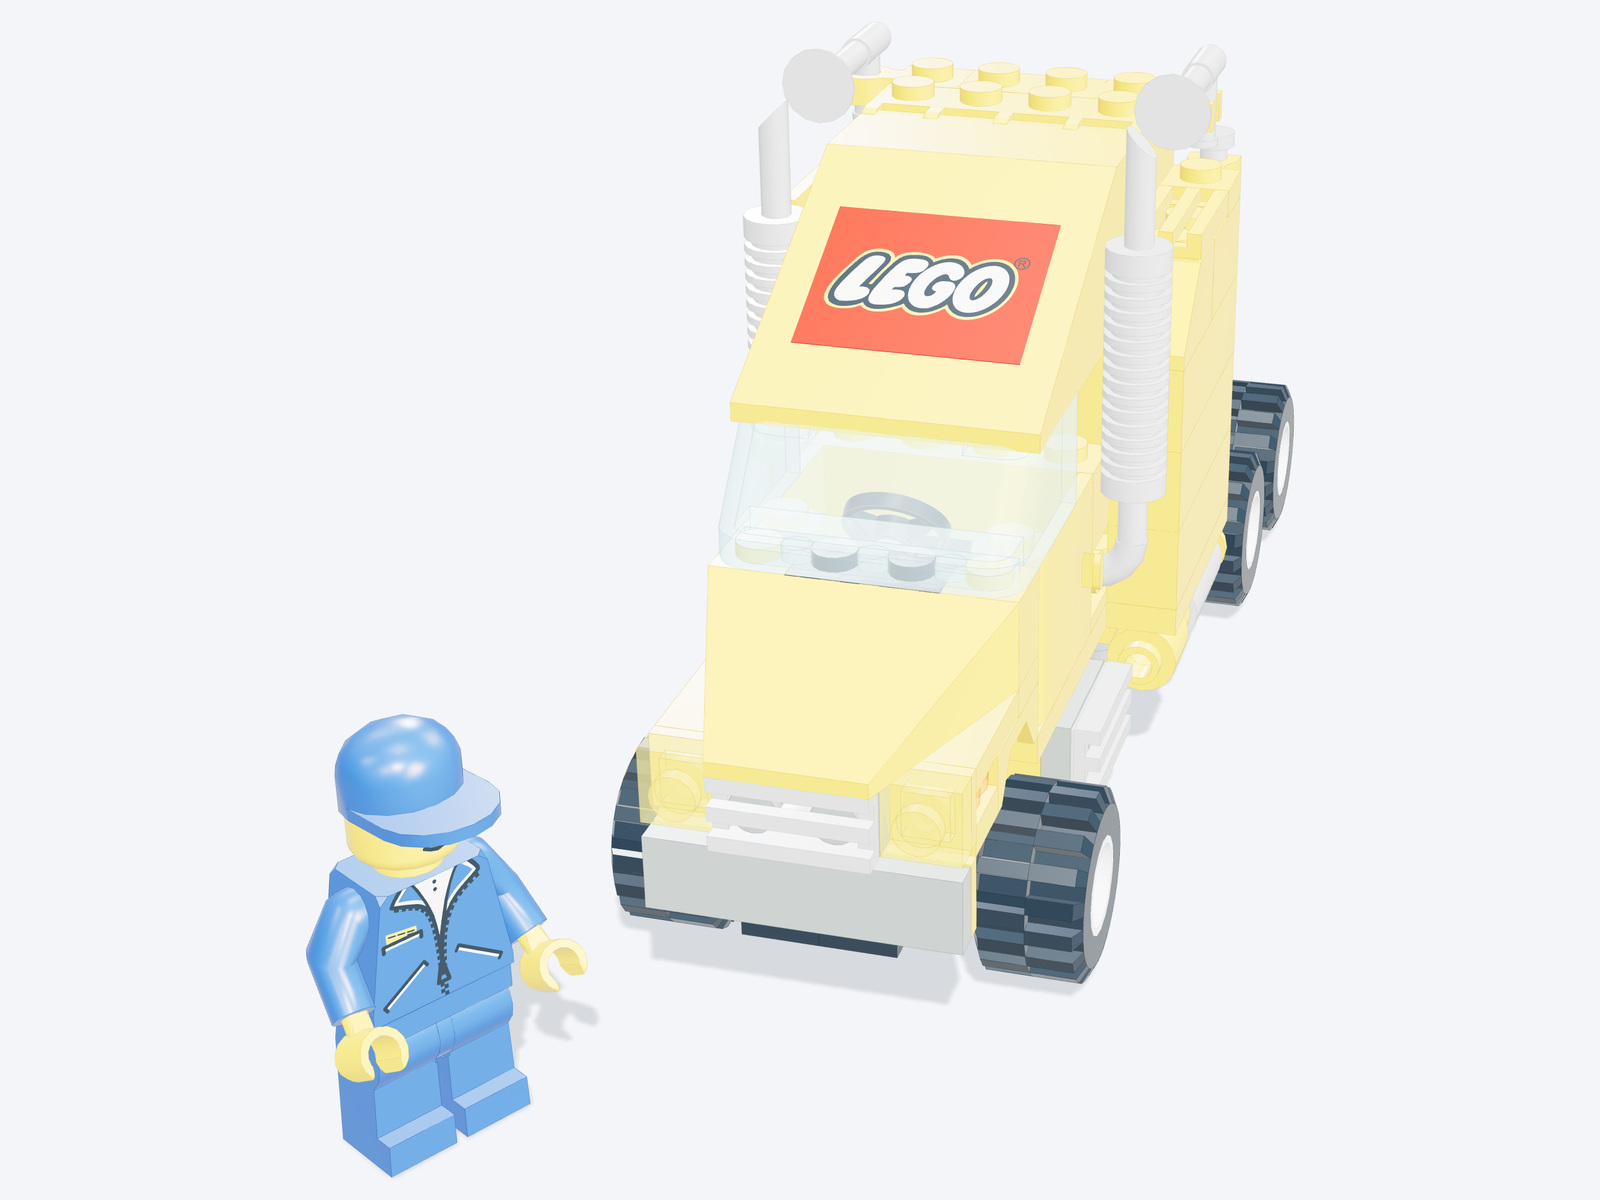
\includegraphics[width=.65\linewidth]{figures-v2/10156-iso.jpg}\end{center}
\paragraph{Attribution.}Robert Paciorek [bercik]. CC BY 2.0.\par\url{https://library.ldraw.org/omr/sets/659}
\paragraph{Source SHA256.}\path{a58a784e6f6ce9d39999db1a4505941b5db5ebd1798af979bae891bc520a1a45}
\paragraph{Connector records.}stud: 213; axle: 13; hinge: 13; fixed: 26; ball: 0
\paragraph{Public input lock.}\path{12d3d37b291161ed18adacf5f133e99539c928536ed76fb5ef1f585f54f5ea01}
\paragraph{Status.}Source preservation does not certify stability. Reference outputs below are internal review material. Full model inputs are the versioned public JSON and numbered PNGs.
\begin{enumerate}
\item \textbf{ld2-10156-color-1}. Identify the original color of B0069; numbered isolation is allowed.
\par{\small color; visual; atomic; single-choice.\par\textit{Operands:} B0069 = brick\_000069\par\textit{Public evidence summary:} Numbered PNG: benchmark/ldraw-v2/inputs/views/ld2-10156-color-1.png; structured input = \{\}.\par\textit{Options:} A: Chrome Silver; B: White; C: Yellow; D: Red\par\textit{Reference output:} \{"choiceId": "C"\}\par\textit{Derivation:} source colorName by rendered B-label; source oracle only\par\textit{Equivalence:} exact declared response\par\textit{Review:} pending required human review.}
\item \textbf{ld2-10156-shape-match-1}. Ignoring color and pose, which numbered instance has the same LDraw part type as B0069?
\par{\small shape-match; visual; atomic; single-choice.\par\textit{Operands:} B0054 = brick\_000054, B0107 = brick\_000107, B0069 = brick\_000069, B0016 = brick\_000016, B0088 = brick\_000088\par\textit{Public evidence summary:} Numbered PNG: benchmark/ldraw-v2/inputs/views/ld2-10156-shape-match-1.png; structured input = \{\}.\par\textit{Options:} A: B0054; B: B0088; C: B0016; D: B0107\par\textit{Reference output:} \{"choiceId": "A"\}\par\textit{Derivation:} source partNumber equality across labeled candidates; source oracle only\par\textit{Equivalence:} same source partNumber; ignore color and pose; perceptual equivalence pending\par\textit{Review:} pending required human review.}
\item \textbf{ld2-10156-distance-1}. Using the supplied geometry bounding-box centers, which candidate is nearest to B0069?
\par{\small distance; source-data; atomic; single-choice.\par\textit{Operands:} B0093 = brick\_000093, B0069 = brick\_000069, B0045 = brick\_000045, B0067 = brick\_000067\par\textit{Public evidence summary:} \{"coordinateFrame": "Viewer world, millimeters, Euclidean distance", "centers": \{"B0069": [68.105528, 47.2, -7.879336], "B0045": [38.606308, 15.2, -36.974207], "B0067": [-3.769975, 28.8, 11.199482], "B0093": [60.18416, 72.8, -26.399917]\}\}\par\textit{Options:} A: B0045; B: B0067; C: B0093\par\textit{Reference output:} \{"choiceId": "C"\}\par\textit{Derivation:} Euclidean norm from public rounded centers\par\textit{Equivalence:} exact declared response\par\textit{Review:} machine checks passed; no human certification.}
\item \textbf{ld2-10156-color-2}. Identify the original color of B0019; numbered isolation is allowed.
\par{\small color; visual; atomic; single-choice.\par\textit{Operands:} B0019 = brick\_000019\par\textit{Public evidence summary:} Numbered PNG: benchmark/ldraw-v2/inputs/views/ld2-10156-color-2.png; structured input = \{\}.\par\textit{Options:} A: Chrome Silver; B: Light Grey; C: Black; D: Trans Neon Orange\par\textit{Reference output:} \{"choiceId": "B"\}\par\textit{Derivation:} source colorName by rendered B-label; source oracle only\par\textit{Equivalence:} exact declared response\par\textit{Review:} pending required human review.}
\item \textbf{ld2-10156-distance-2}. Using the supplied geometry bounding-box centers, which candidate is nearest to B0019?
\par{\small distance; source-data; atomic; single-choice.\par\textit{Operands:} B0031 = brick\_000031, B0019 = brick\_000019, B0086 = brick\_000086, B0101 = brick\_000101\par\textit{Public evidence summary:} \{"coordinateFrame": "Viewer world, millimeters, Euclidean distance", "centers": \{"B0019": [-7.119767, 18.4, 12.499461], "B0086": [65.426448, 48, -52.520376], "B0101": [97.003521, 10.8, -69.827264], "B0031": [38.3926, 15.2, 4.949118]\}\}\par\textit{Options:} A: B0101; B: B0086; C: B0031\par\textit{Reference output:} \{"choiceId": "C"\}\par\textit{Derivation:} Euclidean norm from public rounded centers\par\textit{Equivalence:} exact declared response\par\textit{Review:} machine checks passed; no human certification.}
\item \textbf{ld2-10156-interface-1}. Classify the supplied connector record for B0099 and B0018. This does not certify load capacity.
\par{\small interface; connector-graph; metacognitive; single-choice.\par\textit{Operands:} B0099 = brick\_000099, B0018 = brick\_000018\par\textit{Public evidence summary:} \{"connectorRecord": \{"family": "axle", "aConnector": 0, "bConnector": 1\}, "scope": "Upstream connector tolerances and inset mesh intersections; unknown parts remain explicit, separate scene objects are not glued together; no load/force validation."\}\par\textit{Options:} A: stud; B: axle; C: hinge; D: ball; E: fixed\par\textit{Reference output:} \{"choiceId": "B"\}\par\textit{Derivation:} public connectorRecord.family equality\par\textit{Equivalence:} exact declared response\par\textit{Review:} machine checks passed; no human certification.}
\item \textbf{ld2-10156-interface-2}. Classify the supplied connector record for B0107 and B0108. This does not certify load capacity.
\par{\small interface; connector-graph; metacognitive; single-choice.\par\textit{Operands:} B0107 = brick\_000107, B0108 = brick\_000108\par\textit{Public evidence summary:} \{"connectorRecord": \{"family": "fixed", "aConnector": 2, "bConnector": 1\}, "scope": "Upstream connector tolerances and inset mesh intersections; unknown parts remain explicit, separate scene objects are not glued together; no load/force validation."\}\par\textit{Options:} A: ball; B: fixed; C: hinge; D: axle; E: stud\par\textit{Reference output:} \{"choiceId": "B"\}\par\textit{Derivation:} public connectorRecord.family equality\par\textit{Equivalence:} exact declared response\par\textit{Review:} machine checks passed; no human certification.}
\item \textbf{ld2-10156-interface-3}. Classify the supplied connector record for B0004 and B0010. This does not certify load capacity.
\par{\small interface; connector-graph; metacognitive; single-choice.\par\textit{Operands:} B0004 = brick\_000004, B0010 = brick\_000010\par\textit{Public evidence summary:} \{"connectorRecord": \{"family": "hinge", "aConnector": 2, "bConnector": 1\}, "scope": "Upstream connector tolerances and inset mesh intersections; unknown parts remain explicit, separate scene objects are not glued together; no load/force validation."\}\par\textit{Options:} A: stud; B: hinge; C: ball; D: axle; E: fixed\par\textit{Reference output:} \{"choiceId": "B"\}\par\textit{Derivation:} public connectorRecord.family equality\par\textit{Equivalence:} exact declared response\par\textit{Review:} machine checks passed; no human certification.}
\item \textbf{ld2-10156-interface-4}. Classify the supplied connector record for B0080 and B0088. This does not certify load capacity.
\par{\small interface; connector-graph; metacognitive; single-choice.\par\textit{Operands:} B0088 = brick\_000088, B0080 = brick\_000080\par\textit{Public evidence summary:} \{"connectorRecord": \{"family": "stud", "aConnector": 3, "bConnector": 1\}, "scope": "Upstream connector tolerances and inset mesh intersections; unknown parts remain explicit, separate scene objects are not glued together; no load/force validation."\}\par\textit{Options:} A: ball; B: fixed; C: axle; D: stud; E: hinge\par\textit{Reference output:} \{"choiceId": "D"\}\par\textit{Derivation:} public connectorRecord.family equality\par\textit{Equivalence:} exact declared response\par\textit{Review:} machine checks passed; no human certification.}
\item \textbf{ld2-10156-neighbors-1}. Select every candidate directly adjacent to B0105 in the supplied connector graph.
\par{\small neighbors; connector-graph; metacognitive; multiple-choice.\par\textit{Operands:} B0016 = brick\_000016, B0006 = brick\_000006, B0098 = brick\_000098, B0105 = brick\_000105, B0106 = brick\_000106\par\textit{Public evidence summary:} 2 unique undirected pairs\par\textit{Options:} A: B0006; B: B0098; C: B0016; D: B0106\par\textit{Reference output:} \{"choiceIds": ["C", "D"]\}\par\textit{Derivation:} public incident edge endpoint set\par\textit{Equivalence:} unordered exact set; duplicate IDs invalid\par\textit{Review:} machine checks passed; no human certification.}
\item \textbf{ld2-10156-graph-removal-1}. Delete B0105 and its incident edges from this local graph. How many connected components remain? Do not infer physical extractability.
\par{\small graph-removal; connector-graph; graph-internal; integer.\par\textit{Operands:} B0106 = brick\_000106, B0105 = brick\_000105, B0098 = brick\_000098, B0016 = brick\_000016, B0006 = brick\_000006\par\textit{Public evidence summary:} 2 unique undirected pairs; 5 nodes\par\textit{Reference output:} \{"value": 4\}\par\textit{Derivation:} union-find component count after public target deletion\par\textit{Equivalence:} exact declared response\par\textit{Review:} machine checks passed; no human certification.}
\item \textbf{ld2-10156-neighbors-2}. Select every candidate directly adjacent to B0070 in the supplied connector graph.
\par{\small neighbors; connector-graph; metacognitive; multiple-choice.\par\textit{Operands:} B0070 = brick\_000070, B0082 = brick\_000082, B0063 = brick\_000063, B0035 = brick\_000035, B0076 = brick\_000076\par\textit{Public evidence summary:} 2 unique undirected pairs\par\textit{Options:} A: B0076; B: B0035; C: B0082; D: B0063\par\textit{Reference output:} \{"choiceIds": ["C", "D"]\}\par\textit{Derivation:} public incident edge endpoint set\par\textit{Equivalence:} unordered exact set; duplicate IDs invalid\par\textit{Review:} pending required human review.}
\item \textbf{ld2-10156-graph-removal-2}. Delete B0070 and its incident edges from this local graph. How many connected components remain? Do not infer physical extractability.
\par{\small graph-removal; connector-graph; graph-internal; integer.\par\textit{Operands:} B0070 = brick\_000070, B0063 = brick\_000063, B0082 = brick\_000082, B0035 = brick\_000035, B0076 = brick\_000076\par\textit{Public evidence summary:} 2 unique undirected pairs; 5 nodes\par\textit{Reference output:} \{"value": 4\}\par\textit{Derivation:} union-find component count after public target deletion\par\textit{Equivalence:} exact declared response\par\textit{Review:} pending required human review.}
\item \textbf{ld2-10156-coverage-1}. Which numbered instance lacks a connector definition in the coverage record, so this audit cannot establish that it is floating?
\par{\small coverage; source-data; metacognitive; single-choice.\par\textit{Operands:} B0081 = brick\_000081, B0069 = brick\_000069, B0111 = brick\_000111, B0019 = brick\_000019\par\textit{Public evidence summary:} \{"coverage": [\{"label": "B0081", "supported": true\}, \{"label": "B0019", "supported": true\}, \{"label": "B0111", "supported": false\}, \{"label": "B0069", "supported": true\}]\}\par\textit{Options:} A: B0019; B: B0111; C: B0069; D: B0081\par\textit{Reference output:} \{"choiceId": "B"\}\par\textit{Derivation:} public supported=false record\par\textit{Equivalence:} exact declared response\par\textit{Review:} pending required human review.}
\item \textbf{ld2-10156-evidence-limit-1}. Only source geometry, connector matching and mesh intersection audits are available. Without mass, friction, material or dynamic tests, is gravitational stability established?
\par{\small evidence-limit; source-data; metacognitive; single-choice.\par\textit{Operands:} none\par\textit{Public evidence summary:} \{"available": ["Original CAD", "Connector inference", "Inset-mesh intersection candidates"]\}\par\textit{Options:} A: Not established by this evidence; B: Established\par\textit{Reference output:} \{"choiceId": "A"\}\par\textit{Derivation:} fixed epistemic control label\par\textit{Equivalence:} exact declared response\par\textit{Review:} machine checks passed; no human certification.}
\item \textbf{ld2-10156-source-step-1}. At which expanded author step does B0075 first appear in the supplied source-step table? Source order is not a collision-free assembly proof.
\par{\small source-step; source-data; procedural; single-choice.\par\textit{Operands:} B0001 = brick\_000001, B0075 = brick\_000075\par\textit{Public evidence summary:} 2 supplied author-step records; exact table in public JSON\par\textit{Options:} A: 14; B: 16; C: 11; D: 9\par\textit{Reference output:} \{"choiceId": "A"\}\par\textit{Derivation:} minimum public step index containing target\par\textit{Equivalence:} exact declared response\par\textit{Review:} machine checks passed; no human certification.}
\item \textbf{ld2-10156-source-step-2}. At which expanded author step does B0050 first appear in the supplied source-step table? Source order is not a collision-free assembly proof.
\par{\small source-step; source-data; procedural; single-choice.\par\textit{Operands:} B0001 = brick\_000001, B0050 = brick\_000050\par\textit{Public evidence summary:} 2 supplied author-step records; exact table in public JSON\par\textit{Options:} A: 12; B: 14; C: 19; D: 10\par\textit{Reference output:} \{"choiceId": "D"\}\par\textit{Derivation:} minimum public step index containing target\par\textit{Equivalence:} exact declared response\par\textit{Review:} machine checks passed; no human certification.}
\item \textbf{ld2-10156-source-sequence-1}. Reveal the supplied source-step window in author order. Actions change visibility only, without simulating insertion trajectories.
\par{\small source-sequence; scene-edit; procedural; actions.\par\textit{Operands:} B0004 = brick\_000004, B0010 = brick\_000010, B0011 = brick\_000011, B0020 = brick\_000020, B0017 = brick\_000017, B0019 = brick\_000019, B0003 = brick\_000003, B0002 = brick\_000002, B0025 = brick\_000025, B0021 = brick\_000021, B0006 = brick\_000006, B0023 = brick\_000023, B0024 = brick\_000024, B0009 = brick\_000009, B0013 = brick\_000013, B0026 = brick\_000026, B0007 = brick\_000007, B0028 = brick\_000028, B0001 = brick\_000001, B0027 = brick\_000027, B0016 = brick\_000016, B0008 = brick\_000008, B0022 = brick\_000022, B0014 = brick\_000014, B0029 = brick\_000029, B0012 = brick\_000012, B0005 = brick\_000005, B0018 = brick\_000018, B0015 = brick\_000015\par\textit{Public evidence summary:} 6 public actions; budget 6; \{"initialFacts": ["start"], "goalFacts": ["done-6"], "absentFacts": []\}\par\textit{Reference output:} \{"actionIds": ["step-1", "step-2", "step-3", "step-4", "step-5", "step-6"]\}\par\textit{Derivation:} public precondition solver\par\textit{Equivalence:} any legal sequence reaching all goals within budget; display-only semantics\par\textit{Review:} machine checks passed; no human certification.}
\item \textbf{ld2-10156-restore-instance-1}. The display copy hides B0069. Restore only that numbered instance, preserving all other instances and source poses.
\par{\small restore-instance; scene-edit; procedural; actions.\par\textit{Operands:} B0001 = brick\_000001, B0069 = brick\_000069\par\textit{Public evidence summary:} 2 public actions; budget 1; \{"initialFacts": ["missing-brick\_000069", "present-brick\_000001"], "goalFacts": ["present-brick\_000069", "present-brick\_000001"], "absentFacts": ["missing-brick\_000069"]\}\par\textit{Reference output:} \{"actionIds": ["restore-B0069"]\}\par\textit{Derivation:} public precondition solver\par\textit{Equivalence:} any legal sequence reaching all goals within budget; display-only semantics\par\textit{Review:} machine checks passed; no human certification.}
\item \textbf{ld2-10156-restore-instance-2}. The display copy hides B0019. Restore only that numbered instance, preserving all other instances and source poses.
\par{\small restore-instance; scene-edit; procedural; actions.\par\textit{Operands:} B0019 = brick\_000019, B0001 = brick\_000001\par\textit{Public evidence summary:} 2 public actions; budget 1; \{"initialFacts": ["missing-brick\_000019", "present-brick\_000001"], "goalFacts": ["present-brick\_000019", "present-brick\_000001"], "absentFacts": ["missing-brick\_000019"]\}\par\textit{Reference output:} \{"actionIds": ["restore-B0019"]\}\par\textit{Derivation:} public precondition solver\par\textit{Equivalence:} any legal sequence reaching all goals within budget; display-only semantics\par\textit{Review:} machine checks passed; no human certification.}
\end{enumerate}
\clearpage\section{42102: Mini CLAAS XERION}
129 source instances; 17 tasks; D1 size band. 40 type strings; 11 color codes; 6 unsupported instances; 0 intersection candidates. 56 expanded author steps. Independent reparse: passed.
\begin{center}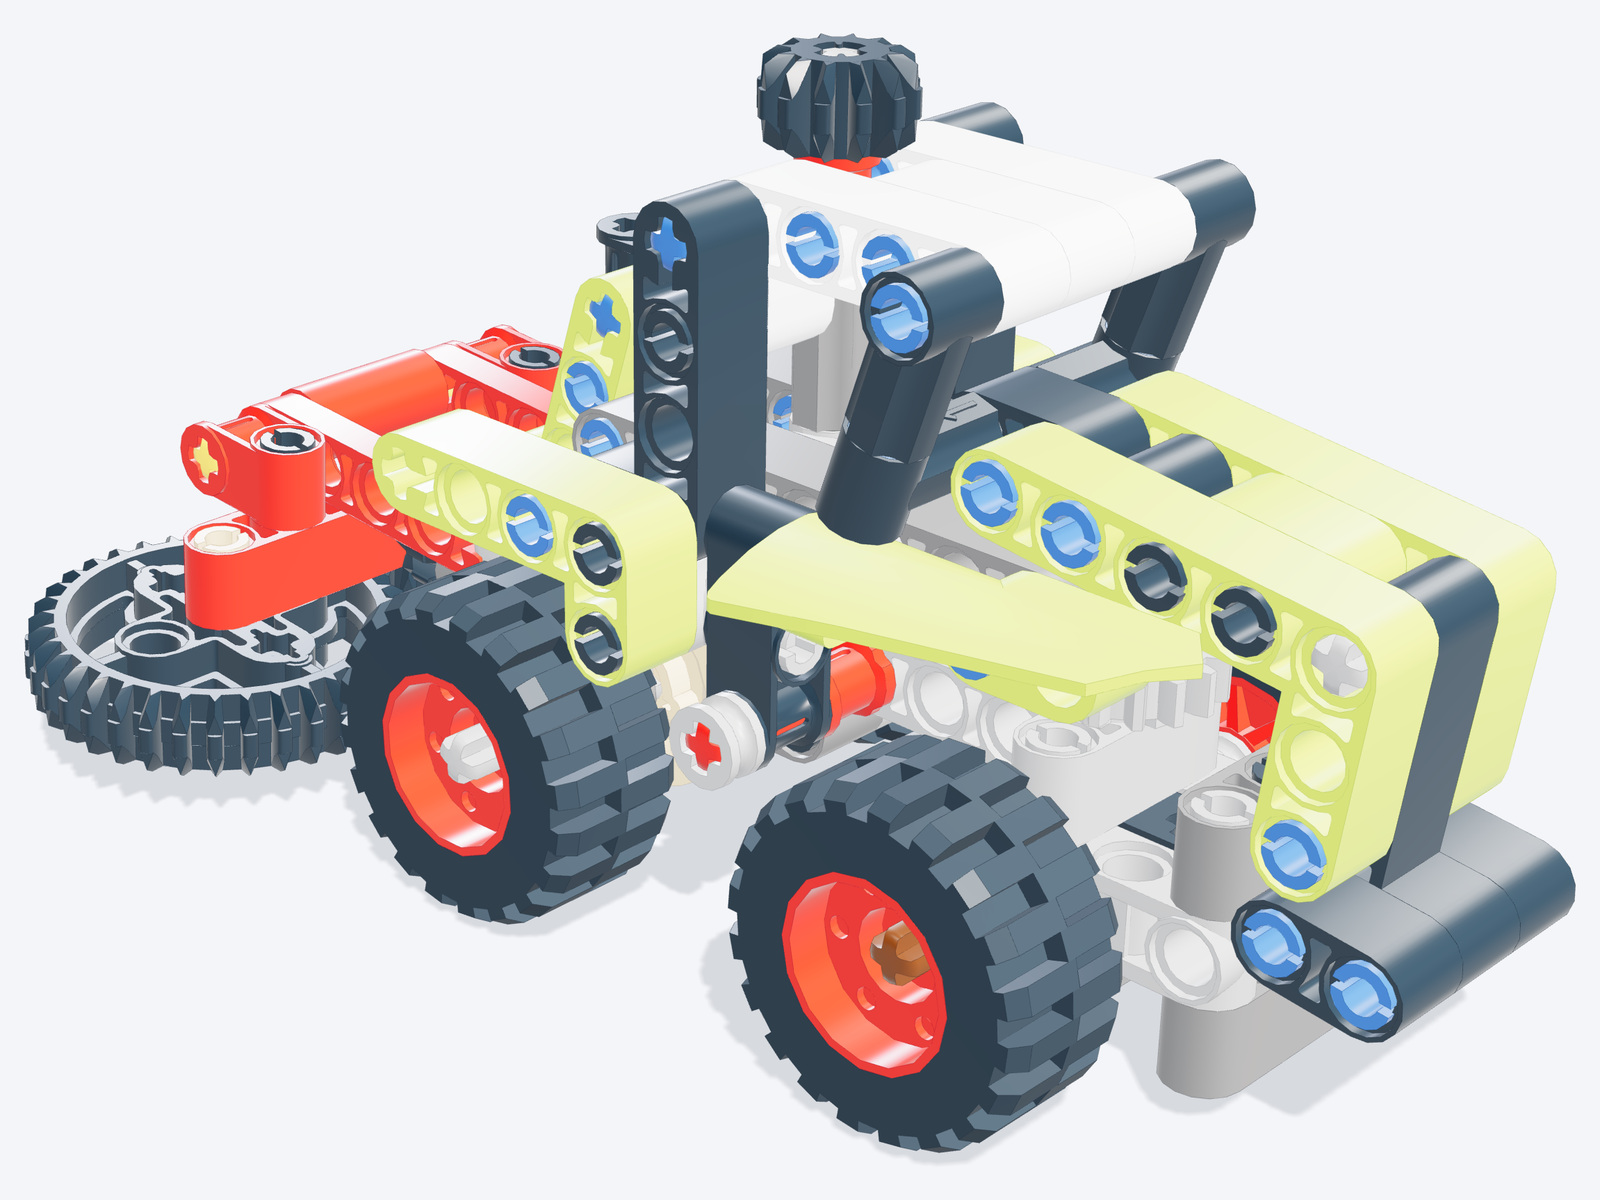
\includegraphics[width=.65\linewidth]{figures-v2/omr-42102-iso.jpg}\end{center}
\paragraph{Attribution.}Max Martin Richter [MMR1988]. CC BY 2.0.\par\url{https://library.ldraw.org/library/omr/42102-1.mpd}
\paragraph{Source SHA256.}\path{096deaf98e20c3e65b547c91e972005d853b1b1c3cf7a619910682e6fe2d2deb}
\paragraph{Connector records.}stud: 0; axle: 152; hinge: 0; fixed: 0; ball: 0
\paragraph{Public input lock.}\path{233161ca642864d13de8219f04b975eb3db1c64f75f2279f803bfd4c40df1f98}
\paragraph{Status.}Source preservation does not certify stability. Reference outputs below are internal review material. Full model inputs are the versioned public JSON and numbered PNGs.
\begin{enumerate}
\item \textbf{ld2-omr-42102-color-1}. Identify the original color of B0094; numbered isolation is allowed.
\par{\small color; visual; atomic; single-choice.\par\textit{Operands:} B0094 = brick\_000094\par\textit{Public evidence summary:} Numbered PNG: benchmark/ldraw-v2/inputs/views/ld2-omr-42102-color-1.png; structured input = \{\}.\par\textit{Options:} A: Black; B: Red; C: Light Bluish Grey; D: Lime\par\textit{Reference output:} \{"choiceId": "D"\}\par\textit{Derivation:} source colorName by rendered B-label; source oracle only\par\textit{Equivalence:} exact declared response\par\textit{Review:} pending required human review.}
\item \textbf{ld2-omr-42102-shape-match-1}. Ignoring color and pose, which numbered instance has the same LDraw part type as B0094?
\par{\small shape-match; visual; atomic; single-choice.\par\textit{Operands:} B0061 = brick\_000061, B0003 = brick\_000003, B0020 = brick\_000020, B0094 = brick\_000094, B0065 = brick\_000065\par\textit{Public evidence summary:} Numbered PNG: benchmark/ldraw-v2/inputs/views/ld2-omr-42102-shape-match-1.png; structured input = \{\}.\par\textit{Options:} A: B0003; B: B0020; C: B0061; D: B0065\par\textit{Reference output:} \{"choiceId": "C"\}\par\textit{Derivation:} source partNumber equality across labeled candidates; source oracle only\par\textit{Equivalence:} same source partNumber; ignore color and pose; perceptual equivalence pending\par\textit{Review:} pending required human review.}
\item \textbf{ld2-omr-42102-distance-1}. Using the supplied geometry bounding-box centers, which candidate is nearest to B0094?
\par{\small distance; source-data; atomic; single-choice.\par\textit{Operands:} B0094 = brick\_000094, B0019 = brick\_000019, B0053 = brick\_000053, B0045 = brick\_000045\par\textit{Public evidence summary:} \{"coordinateFrame": "Viewer world, millimeters, Euclidean distance", "centers": \{"B0094": [8, 20.569662, -71.488617], "B0045": [8, 28.592, 18.5592], "B0019": [12, 32, -56], "B0053": [8, 32.496, -13.2168]\}\}\par\textit{Options:} A: B0045; B: B0053; C: B0019\par\textit{Reference output:} \{"choiceId": "C"\}\par\textit{Derivation:} Euclidean norm from public rounded centers\par\textit{Equivalence:} exact declared response\par\textit{Review:} machine checks passed; no human certification.}
\item \textbf{ld2-omr-42102-color-2}. Identify the original color of B0088; numbered isolation is allowed.
\par{\small color; visual; atomic; single-choice.\par\textit{Operands:} B0088 = brick\_000088\par\textit{Public evidence summary:} Numbered PNG: benchmark/ldraw-v2/inputs/views/ld2-omr-42102-color-2.png; structured input = \{\}.\par\textit{Options:} A: Black; B: Lime; C: Tan; D: Dark Bluish Grey\par\textit{Reference output:} \{"choiceId": "A"\}\par\textit{Derivation:} source colorName by rendered B-label; source oracle only\par\textit{Equivalence:} exact declared response\par\textit{Review:} pending required human review.}
\item \textbf{ld2-omr-42102-distance-2}. Using the supplied geometry bounding-box centers, which candidate is nearest to B0088?
\par{\small distance; source-data; atomic; single-choice.\par\textit{Operands:} B0088 = brick\_000088, B0113 = brick\_000113, B0124 = brick\_000124, B0059 = brick\_000059\par\textit{Public evidence summary:} \{"coordinateFrame": "Viewer world, millimeters, Euclidean distance", "centers": \{"B0088": [8, 1.4752, -75.9456], "B0113": [6, -0.0048, -56.0056], "B0059": [28, 16, -40], "B0124": [31.4, 0, -8]\}\}\par\textit{Options:} A: B0113; B: B0124; C: B0059\par\textit{Reference output:} \{"choiceId": "A"\}\par\textit{Derivation:} Euclidean norm from public rounded centers\par\textit{Equivalence:} exact declared response\par\textit{Review:} machine checks passed; no human certification.}
\item \textbf{ld2-omr-42102-interface-1}. Classify the supplied connector record for B0037 and B0040. This does not certify load capacity.
\par{\small interface; connector-graph; metacognitive; single-choice.\par\textit{Operands:} B0037 = brick\_000037, B0040 = brick\_000040\par\textit{Public evidence summary:} \{"connectorRecord": \{"family": "axle", "aConnector": 2, "bConnector": 1\}, "scope": "Upstream connector tolerances and inset mesh intersections; unknown parts remain explicit, separate scene objects are not glued together; no load/force validation."\}\par\textit{Options:} A: hinge; B: axle; C: stud; D: fixed; E: ball\par\textit{Reference output:} \{"choiceId": "B"\}\par\textit{Derivation:} public connectorRecord.family equality\par\textit{Equivalence:} exact declared response\par\textit{Review:} machine checks passed; no human certification.}
\item \textbf{ld2-omr-42102-neighbors-1}. Select every candidate directly adjacent to B0118 in the supplied connector graph.
\par{\small neighbors; connector-graph; metacognitive; multiple-choice.\par\textit{Operands:} B0091 = brick\_000091, B0118 = brick\_000118, B0055 = brick\_000055, B0013 = brick\_000013, B0119 = brick\_000119\par\textit{Public evidence summary:} 2 unique undirected pairs\par\textit{Options:} A: B0055; B: B0119; C: B0091; D: B0013\par\textit{Reference output:} \{"choiceIds": ["B", "D"]\}\par\textit{Derivation:} public incident edge endpoint set\par\textit{Equivalence:} unordered exact set; duplicate IDs invalid\par\textit{Review:} pending required human review.}
\item \textbf{ld2-omr-42102-graph-removal-1}. Delete B0118 and its incident edges from this local graph. How many connected components remain? Do not infer physical extractability.
\par{\small graph-removal; connector-graph; graph-internal; integer.\par\textit{Operands:} B0119 = brick\_000119, B0013 = brick\_000013, B0091 = brick\_000091, B0118 = brick\_000118, B0055 = brick\_000055\par\textit{Public evidence summary:} 2 unique undirected pairs; 5 nodes\par\textit{Reference output:} \{"value": 4\}\par\textit{Derivation:} union-find component count after public target deletion\par\textit{Equivalence:} exact declared response\par\textit{Review:} pending required human review.}
\item \textbf{ld2-omr-42102-neighbors-2}. Select every candidate directly adjacent to B0075 in the supplied connector graph.
\par{\small neighbors; connector-graph; metacognitive; multiple-choice.\par\textit{Operands:} B0129 = brick\_000129, B0120 = brick\_000120, B0075 = brick\_000075, B0074 = brick\_000074, B0071 = brick\_000071\par\textit{Public evidence summary:} 2 unique undirected pairs\par\textit{Options:} A: B0120; B: B0071; C: B0074; D: B0129\par\textit{Reference output:} \{"choiceIds": ["B", "C"]\}\par\textit{Derivation:} public incident edge endpoint set\par\textit{Equivalence:} unordered exact set; duplicate IDs invalid\par\textit{Review:} pending required human review.}
\item \textbf{ld2-omr-42102-graph-removal-2}. Delete B0075 and its incident edges from this local graph. How many connected components remain? Do not infer physical extractability.
\par{\small graph-removal; connector-graph; graph-internal; integer.\par\textit{Operands:} B0120 = brick\_000120, B0071 = brick\_000071, B0075 = brick\_000075, B0129 = brick\_000129, B0074 = brick\_000074\par\textit{Public evidence summary:} 2 unique undirected pairs; 5 nodes\par\textit{Reference output:} \{"value": 4\}\par\textit{Derivation:} union-find component count after public target deletion\par\textit{Equivalence:} exact declared response\par\textit{Review:} pending required human review.}
\item \textbf{ld2-omr-42102-coverage-1}. Which numbered instance lacks a connector definition in the coverage record, so this audit cannot establish that it is floating?
\par{\small coverage; source-data; metacognitive; single-choice.\par\textit{Operands:} B0114 = brick\_000114, B0094 = brick\_000094, B0009 = brick\_000009, B0088 = brick\_000088\par\textit{Public evidence summary:} \{"coverage": [\{"label": "B0088", "supported": true\}, \{"label": "B0114", "supported": true\}, \{"label": "B0009", "supported": false\}, \{"label": "B0094", "supported": true\}]\}\par\textit{Options:} A: B0009; B: B0094; C: B0114; D: B0088\par\textit{Reference output:} \{"choiceId": "A"\}\par\textit{Derivation:} public supported=false record\par\textit{Equivalence:} exact declared response\par\textit{Review:} pending required human review.}
\item \textbf{ld2-omr-42102-evidence-limit-1}. Only source geometry, connector matching and mesh intersection audits are available. Without mass, friction, material or dynamic tests, is gravitational stability established?
\par{\small evidence-limit; source-data; metacognitive; single-choice.\par\textit{Operands:} none\par\textit{Public evidence summary:} \{"available": ["Original CAD", "Connector inference", "Inset-mesh intersection candidates"]\}\par\textit{Options:} A: Established; B: Not established by this evidence\par\textit{Reference output:} \{"choiceId": "B"\}\par\textit{Derivation:} fixed epistemic control label\par\textit{Equivalence:} exact declared response\par\textit{Review:} machine checks passed; no human certification.}
\item \textbf{ld2-omr-42102-source-step-1}. At which expanded author step does B0094 first appear in the supplied source-step table? Source order is not a collision-free assembly proof.
\par{\small source-step; source-data; procedural; single-choice.\par\textit{Operands:} B0001 = brick\_000001, B0094 = brick\_000094\par\textit{Public evidence summary:} 2 supplied author-step records; exact table in public JSON\par\textit{Options:} A: 22; B: 43; C: 52; D: 55\par\textit{Reference output:} \{"choiceId": "B"\}\par\textit{Derivation:} minimum public step index containing target\par\textit{Equivalence:} exact declared response\par\textit{Review:} machine checks passed; no human certification.}
\item \textbf{ld2-omr-42102-source-step-2}. At which expanded author step does B0078 first appear in the supplied source-step table? Source order is not a collision-free assembly proof.
\par{\small source-step; source-data; procedural; single-choice.\par\textit{Operands:} B0078 = brick\_000078, B0001 = brick\_000001\par\textit{Public evidence summary:} 2 supplied author-step records; exact table in public JSON\par\textit{Options:} A: 35; B: 11; C: 16; D: 17\par\textit{Reference output:} \{"choiceId": "A"\}\par\textit{Derivation:} minimum public step index containing target\par\textit{Equivalence:} exact declared response\par\textit{Review:} machine checks passed; no human certification.}
\item \textbf{ld2-omr-42102-source-sequence-1}. Reveal the supplied source-step window in author order. Actions change visibility only, without simulating insertion trajectories.
\par{\small source-sequence; scene-edit; procedural; actions.\par\textit{Operands:} B0001 = brick\_000001, B0010 = brick\_000010, B0014 = brick\_000014, B0012 = brick\_000012, B0011 = brick\_000011, B0003 = brick\_000003, B0002 = brick\_000002, B0004 = brick\_000004, B0013 = brick\_000013, B0005 = brick\_000005, B0009 = brick\_000009, B0008 = brick\_000008, B0007 = brick\_000007, B0006 = brick\_000006\par\textit{Public evidence summary:} 6 public actions; budget 6; \{"initialFacts": ["start"], "goalFacts": ["done-6"], "absentFacts": []\}\par\textit{Reference output:} \{"actionIds": ["step-1", "step-2", "step-3", "step-4", "step-5", "step-6"]\}\par\textit{Derivation:} public precondition solver\par\textit{Equivalence:} any legal sequence reaching all goals within budget; display-only semantics\par\textit{Review:} pending required human review.}
\item \textbf{ld2-omr-42102-restore-instance-1}. The display copy hides B0094. Restore only that numbered instance, preserving all other instances and source poses.
\par{\small restore-instance; scene-edit; procedural; actions.\par\textit{Operands:} B0001 = brick\_000001, B0094 = brick\_000094\par\textit{Public evidence summary:} 2 public actions; budget 1; \{"initialFacts": ["missing-brick\_000094", "present-brick\_000001"], "goalFacts": ["present-brick\_000094", "present-brick\_000001"], "absentFacts": ["missing-brick\_000094"]\}\par\textit{Reference output:} \{"actionIds": ["restore-B0094"]\}\par\textit{Derivation:} public precondition solver\par\textit{Equivalence:} any legal sequence reaching all goals within budget; display-only semantics\par\textit{Review:} machine checks passed; no human certification.}
\item \textbf{ld2-omr-42102-restore-instance-2}. The display copy hides B0088. Restore only that numbered instance, preserving all other instances and source poses.
\par{\small restore-instance; scene-edit; procedural; actions.\par\textit{Operands:} B0088 = brick\_000088, B0001 = brick\_000001\par\textit{Public evidence summary:} 2 public actions; budget 1; \{"initialFacts": ["missing-brick\_000088", "present-brick\_000001"], "goalFacts": ["present-brick\_000088", "present-brick\_000001"], "absentFacts": ["missing-brick\_000088"]\}\par\textit{Reference output:} \{"actionIds": ["restore-B0088"]\}\par\textit{Derivation:} public precondition solver\par\textit{Equivalence:} any legal sequence reaching all goals within budget; display-only semantics\par\textit{Review:} machine checks passed; no human certification.}
\end{enumerate}
\clearpage\section{42020: Twin-Rotor Helicopter}
141 source instances; 14 tasks; D1 size band. 45 type strings; 8 color codes; 0 unsupported instances; 0 intersection candidates. 0 expanded author steps. Independent reparse: passed.
\begin{center}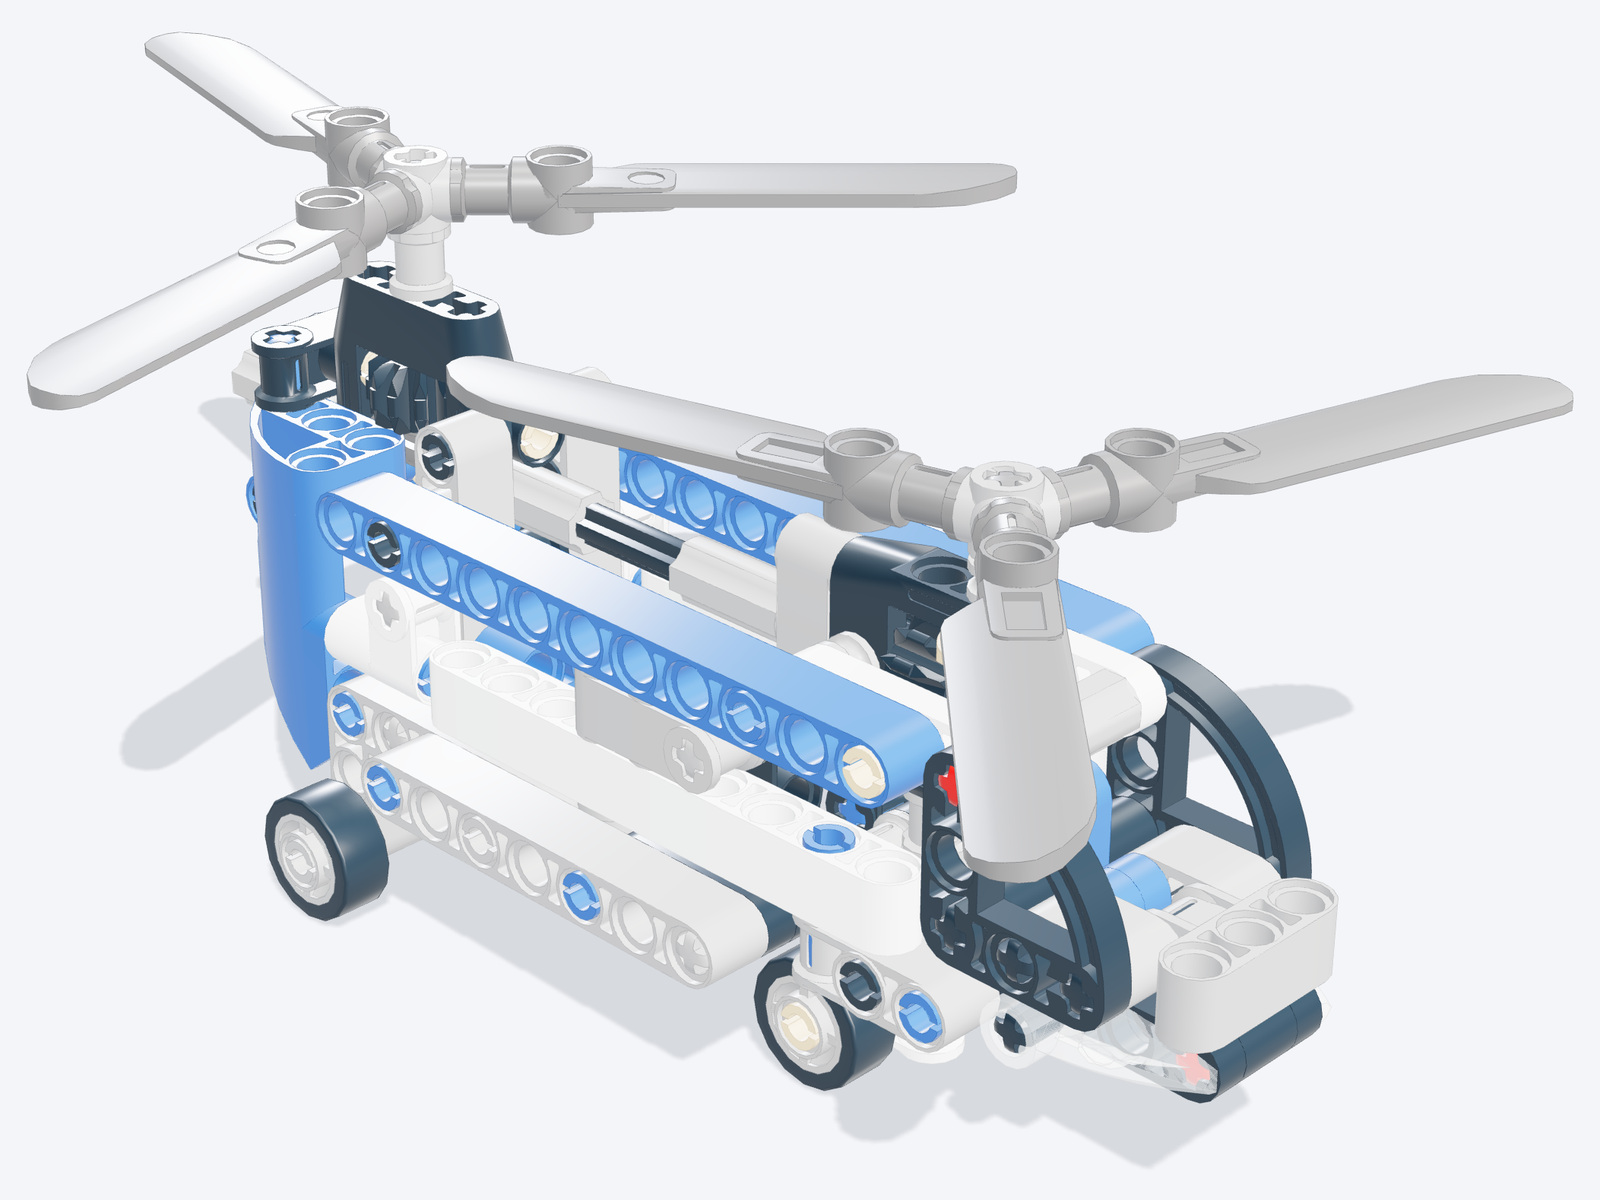
\includegraphics[width=.65\linewidth]{figures-v2/omr-42020-iso.jpg}\end{center}
\paragraph{Attribution.}Faramond Florent [Makou]. CC BY 2.0.\par\url{https://library.ldraw.org/library/omr/42020-1.mpd}
\paragraph{Source SHA256.}\path{03ce9e9f6e5e8fe9b35ec612407be6ac51996d369a341775b5ae80b45d7017a2}
\paragraph{Connector records.}stud: 0; axle: 181; hinge: 0; fixed: 16; ball: 0
\paragraph{Public input lock.}\path{8d837ec764a1e894d4e133636396377ebda7d89e796f297d18b746bb8a6ee733}
\paragraph{Status.}Source preservation does not certify stability. Reference outputs below are internal review material. Full model inputs are the versioned public JSON and numbered PNGs.
\begin{enumerate}
\item \textbf{ld2-omr-42020-color-1}. Identify the original color of B0064; numbered isolation is allowed.
\par{\small color; visual; atomic; single-choice.\par\textit{Operands:} B0064 = brick\_000064\par\textit{Public evidence summary:} Numbered PNG: benchmark/ldraw-v2/inputs/views/ld2-omr-42020-color-1.png; structured input = \{\}.\par\textit{Options:} A: Dark Bluish Grey; B: Light Bluish Grey; C: Red; D: Black\par\textit{Reference output:} \{"choiceId": "B"\}\par\textit{Derivation:} source colorName by rendered B-label; source oracle only\par\textit{Equivalence:} exact declared response\par\textit{Review:} pending required human review.}
\item \textbf{ld2-omr-42020-shape-match-1}. Ignoring color and pose, which numbered instance has the same LDraw part type as B0064?
\par{\small shape-match; visual; atomic; single-choice.\par\textit{Operands:} B0120 = brick\_000120, B0117 = brick\_000117, B0064 = brick\_000064, B0109 = brick\_000109, B0063 = brick\_000063\par\textit{Public evidence summary:} Numbered PNG: benchmark/ldraw-v2/inputs/views/ld2-omr-42020-shape-match-1.png; structured input = \{\}.\par\textit{Options:} A: B0109; B: B0120; C: B0117; D: B0063\par\textit{Reference output:} \{"choiceId": "D"\}\par\textit{Derivation:} source partNumber equality across labeled candidates; source oracle only\par\textit{Equivalence:} same source partNumber; ignore color and pose; perceptual equivalence pending\par\textit{Review:} pending required human review.}
\item \textbf{ld2-omr-42020-distance-1}. Using the supplied geometry bounding-box centers, which candidate is nearest to B0064?
\par{\small distance; source-data; atomic; single-choice.\par\textit{Operands:} B0107 = brick\_000107, B0053 = brick\_000053, B0064 = brick\_000064, B0051 = brick\_000051\par\textit{Public evidence summary:} \{"coordinateFrame": "Viewer world, millimeters, Euclidean distance", "centers": \{"B0064": [16, -40, -20], "B0053": [32, -48, -8], "B0107": [22, -16, 88], "B0051": [-3.8, -23.2, -23.800047]\}\}\par\textit{Options:} A: B0107; B: B0053; C: B0051\par\textit{Reference output:} \{"choiceId": "B"\}\par\textit{Derivation:} Euclidean norm from public rounded centers\par\textit{Equivalence:} exact declared response\par\textit{Review:} machine checks passed; no human certification.}
\item \textbf{ld2-omr-42020-color-2}. Identify the original color of B0030; numbered isolation is allowed.
\par{\small color; visual; atomic; single-choice.\par\textit{Operands:} B0030 = brick\_000030\par\textit{Public evidence summary:} Numbered PNG: benchmark/ldraw-v2/inputs/views/ld2-omr-42020-color-2.png; structured input = \{\}.\par\textit{Options:} A: Red; B: Light Bluish Grey; C: Dark Bluish Grey; D: White\par\textit{Reference output:} \{"choiceId": "B"\}\par\textit{Derivation:} source colorName by rendered B-label; source oracle only\par\textit{Equivalence:} exact declared response\par\textit{Review:} pending required human review.}
\item \textbf{ld2-omr-42020-distance-2}. Using the supplied geometry bounding-box centers, which candidate is nearest to B0030?
\par{\small distance; source-data; atomic; single-choice.\par\textit{Operands:} B0052 = brick\_000052, B0017 = brick\_000017, B0132 = brick\_000132, B0030 = brick\_000030\par\textit{Public evidence summary:} \{"coordinateFrame": "Viewer world, millimeters, Euclidean distance", "centers": \{"B0030": [8, -32, 24], "B0132": [0, -24, 92], "B0052": [8, -16, -32], "B0017": [24, -32, 8]\}\}\par\textit{Options:} A: B0132; B: B0052; C: B0017\par\textit{Reference output:} \{"choiceId": "C"\}\par\textit{Derivation:} Euclidean norm from public rounded centers\par\textit{Equivalence:} exact declared response\par\textit{Review:} machine checks passed; no human certification.}
\item \textbf{ld2-omr-42020-interface-1}. Classify the supplied connector record for B0004 and B0005. This does not certify load capacity.
\par{\small interface; connector-graph; metacognitive; single-choice.\par\textit{Operands:} B0005 = brick\_000005, B0004 = brick\_000004\par\textit{Public evidence summary:} \{"connectorRecord": \{"family": "axle", "aConnector": 0, "bConnector": 0\}, "scope": "Upstream connector tolerances and inset mesh intersections; unknown parts remain explicit, separate scene objects are not glued together; no load/force validation."\}\par\textit{Options:} A: ball; B: fixed; C: hinge; D: axle; E: stud\par\textit{Reference output:} \{"choiceId": "D"\}\par\textit{Derivation:} public connectorRecord.family equality\par\textit{Equivalence:} exact declared response\par\textit{Review:} machine checks passed; no human certification.}
\item \textbf{ld2-omr-42020-interface-2}. Classify the supplied connector record for B0053 and B0059. This does not certify load capacity.
\par{\small interface; connector-graph; metacognitive; single-choice.\par\textit{Operands:} B0059 = brick\_000059, B0053 = brick\_000053\par\textit{Public evidence summary:} \{"connectorRecord": \{"family": "fixed", "aConnector": 1, "bConnector": 0\}, "scope": "Upstream connector tolerances and inset mesh intersections; unknown parts remain explicit, separate scene objects are not glued together; no load/force validation."\}\par\textit{Options:} A: ball; B: fixed; C: stud; D: axle; E: hinge\par\textit{Reference output:} \{"choiceId": "B"\}\par\textit{Derivation:} public connectorRecord.family equality\par\textit{Equivalence:} exact declared response\par\textit{Review:} machine checks passed; no human certification.}
\item \textbf{ld2-omr-42020-neighbors-1}. Select every candidate directly adjacent to B0007 in the supplied connector graph.
\par{\small neighbors; connector-graph; metacognitive; multiple-choice.\par\textit{Operands:} B0035 = brick\_000035, B0007 = brick\_000007, B0012 = brick\_000012, B0086 = brick\_000086, B0023 = brick\_000023\par\textit{Public evidence summary:} 2 unique undirected pairs\par\textit{Options:} A: B0012; B: B0023; C: B0035; D: B0086\par\textit{Reference output:} \{"choiceIds": ["A", "C"]\}\par\textit{Derivation:} public incident edge endpoint set\par\textit{Equivalence:} unordered exact set; duplicate IDs invalid\par\textit{Review:} machine checks passed; no human certification.}
\item \textbf{ld2-omr-42020-graph-removal-1}. Delete B0007 and its incident edges from this local graph. How many connected components remain? Do not infer physical extractability.
\par{\small graph-removal; connector-graph; graph-internal; integer.\par\textit{Operands:} B0012 = brick\_000012, B0086 = brick\_000086, B0035 = brick\_000035, B0023 = brick\_000023, B0007 = brick\_000007\par\textit{Public evidence summary:} 2 unique undirected pairs; 5 nodes\par\textit{Reference output:} \{"value": 4\}\par\textit{Derivation:} union-find component count after public target deletion\par\textit{Equivalence:} exact declared response\par\textit{Review:} machine checks passed; no human certification.}
\item \textbf{ld2-omr-42020-neighbors-2}. Select every candidate directly adjacent to B0079 in the supplied connector graph.
\par{\small neighbors; connector-graph; metacognitive; multiple-choice.\par\textit{Operands:} B0113 = brick\_000113, B0079 = brick\_000079, B0059 = brick\_000059, B0075 = brick\_000075, B0081 = brick\_000081\par\textit{Public evidence summary:} 2 unique undirected pairs\par\textit{Options:} A: B0081; B: B0059; C: B0075; D: B0113\par\textit{Reference output:} \{"choiceIds": ["A", "C"]\}\par\textit{Derivation:} public incident edge endpoint set\par\textit{Equivalence:} unordered exact set; duplicate IDs invalid\par\textit{Review:} machine checks passed; no human certification.}
\item \textbf{ld2-omr-42020-graph-removal-2}. Delete B0079 and its incident edges from this local graph. How many connected components remain? Do not infer physical extractability.
\par{\small graph-removal; connector-graph; graph-internal; integer.\par\textit{Operands:} B0081 = brick\_000081, B0113 = brick\_000113, B0059 = brick\_000059, B0079 = brick\_000079, B0075 = brick\_000075\par\textit{Public evidence summary:} 2 unique undirected pairs; 5 nodes\par\textit{Reference output:} \{"value": 4\}\par\textit{Derivation:} union-find component count after public target deletion\par\textit{Equivalence:} exact declared response\par\textit{Review:} machine checks passed; no human certification.}
\item \textbf{ld2-omr-42020-evidence-limit-1}. Only source geometry, connector matching and mesh intersection audits are available. Without mass, friction, material or dynamic tests, is gravitational stability established?
\par{\small evidence-limit; source-data; metacognitive; single-choice.\par\textit{Operands:} none\par\textit{Public evidence summary:} \{"available": ["Original CAD", "Connector inference", "Inset-mesh intersection candidates"]\}\par\textit{Options:} A: Not established by this evidence; B: Established\par\textit{Reference output:} \{"choiceId": "A"\}\par\textit{Derivation:} fixed epistemic control label\par\textit{Equivalence:} exact declared response\par\textit{Review:} machine checks passed; no human certification.}
\item \textbf{ld2-omr-42020-restore-instance-1}. The display copy hides B0064. Restore only that numbered instance, preserving all other instances and source poses.
\par{\small restore-instance; scene-edit; procedural; actions.\par\textit{Operands:} B0001 = brick\_000001, B0064 = brick\_000064\par\textit{Public evidence summary:} 2 public actions; budget 1; \{"initialFacts": ["missing-brick\_000064", "present-brick\_000001"], "goalFacts": ["present-brick\_000064", "present-brick\_000001"], "absentFacts": ["missing-brick\_000064"]\}\par\textit{Reference output:} \{"actionIds": ["restore-B0064"]\}\par\textit{Derivation:} public precondition solver\par\textit{Equivalence:} any legal sequence reaching all goals within budget; display-only semantics\par\textit{Review:} machine checks passed; no human certification.}
\item \textbf{ld2-omr-42020-restore-instance-2}. The display copy hides B0030. Restore only that numbered instance, preserving all other instances and source poses.
\par{\small restore-instance; scene-edit; procedural; actions.\par\textit{Operands:} B0030 = brick\_000030, B0001 = brick\_000001\par\textit{Public evidence summary:} 2 public actions; budget 1; \{"initialFacts": ["missing-brick\_000030", "present-brick\_000001"], "goalFacts": ["present-brick\_000030", "present-brick\_000001"], "absentFacts": ["missing-brick\_000030"]\}\par\textit{Reference output:} \{"actionIds": ["restore-B0030"]\}\par\textit{Derivation:} public precondition solver\par\textit{Equivalence:} any legal sequence reaching all goals within budget; display-only semantics\par\textit{Review:} machine checks passed; no human certification.}
\end{enumerate}
\clearpage\section{10036: Pizza To Go}
166 source instances; 20 tasks; D2 size band. 71 type strings; 12 color codes; 0 unsupported instances; 3 intersection candidates. 29 expanded author steps. Independent reparse: passed.
\begin{center}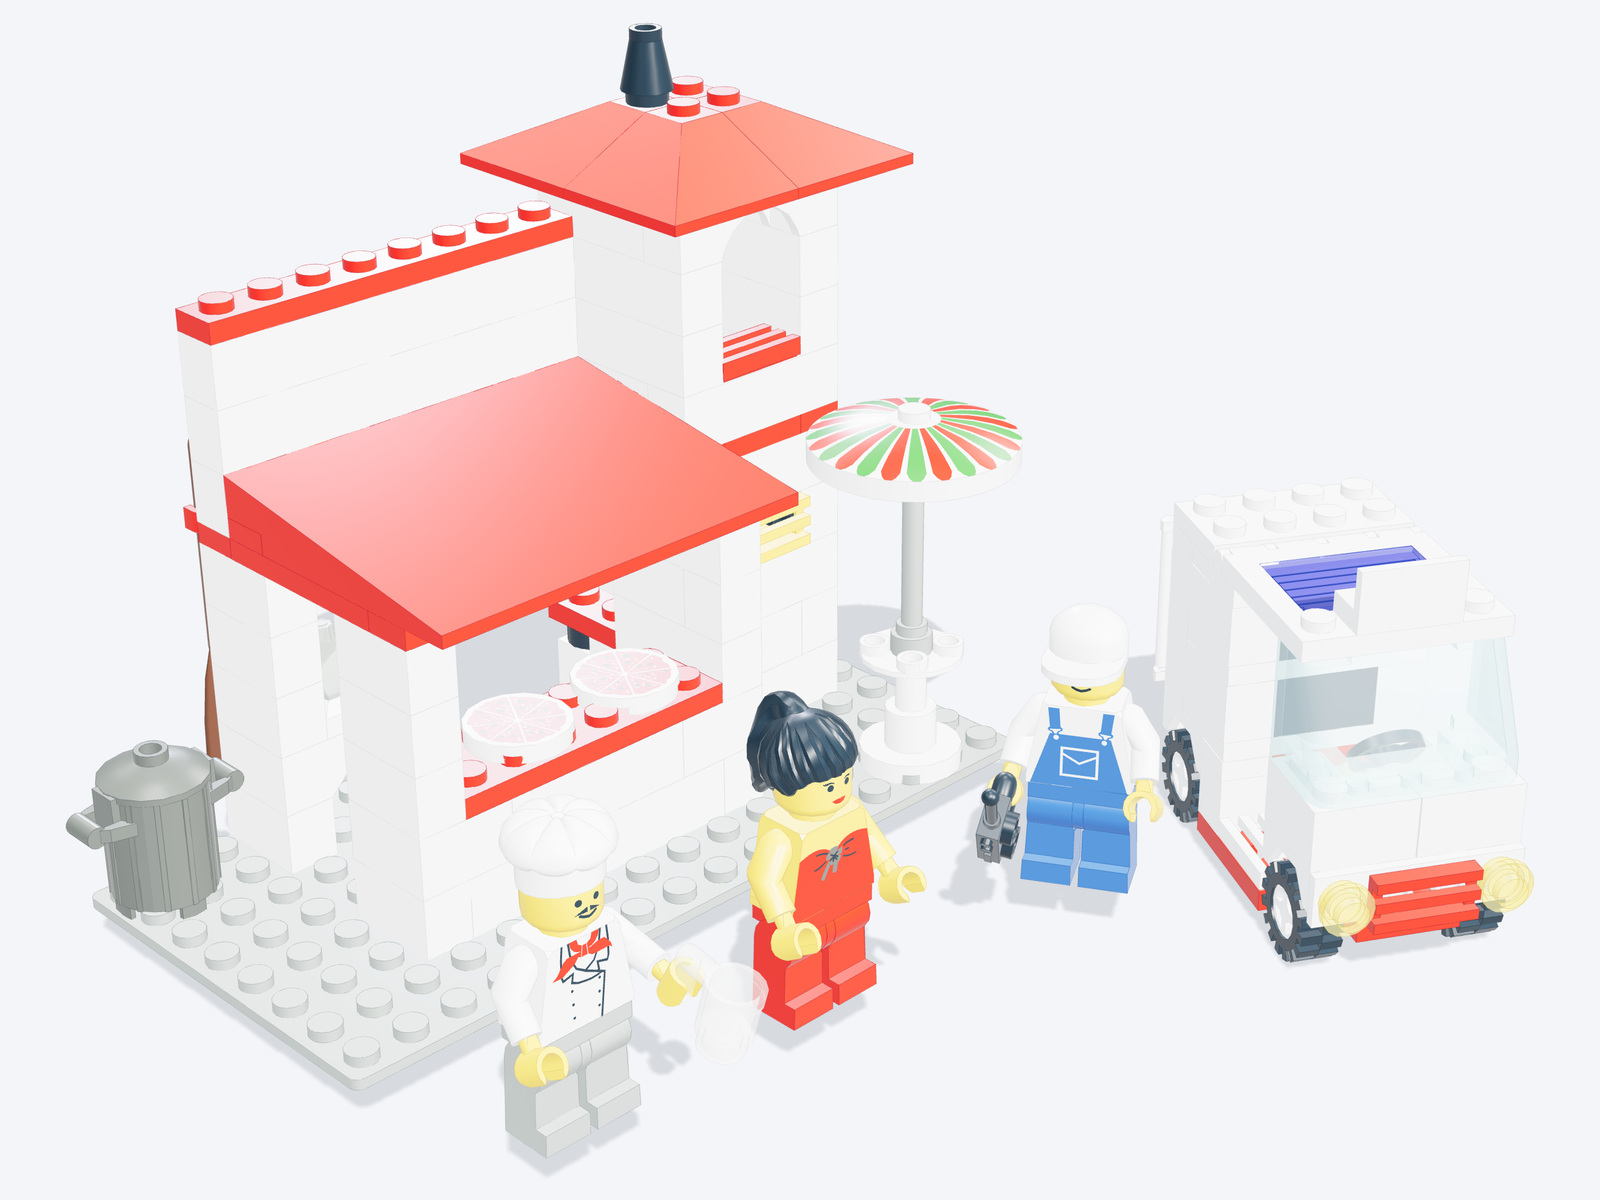
\includegraphics[width=.65\linewidth]{figures-v2/10036-iso.jpg}\end{center}
\paragraph{Attribution.}Robert Paciorek [bercik]. CC BY 2.0.\par\url{https://library.ldraw.org/omr/sets/658}
\paragraph{Source SHA256.}\path{bb9eafb3fc283a4b3b28eef58d6f9208528ee3d9b3debe4a7db8bbadc85f63f8}
\paragraph{Connector records.}stud: 361; axle: 11; hinge: 24; fixed: 22; ball: 0
\paragraph{Public input lock.}\path{d897373fa4507a329b51bf19d067a8237781e3c2504acce2db5b2903523db9a3}
\paragraph{Status.}Source preservation does not certify stability. Reference outputs below are internal review material. Full model inputs are the versioned public JSON and numbered PNGs.
\begin{enumerate}
\item \textbf{ld2-10036-color-1}. Identify the original color of B0063; numbered isolation is allowed.
\par{\small color; visual; atomic; single-choice.\par\textit{Operands:} B0063 = brick\_000063\par\textit{Public evidence summary:} Numbered PNG: benchmark/ldraw-v2/inputs/views/ld2-10036-color-1.png; structured input = \{\}.\par\textit{Options:} A: Trans Light Blue; B: White; C: Brown; D: Dark Grey\par\textit{Reference output:} \{"choiceId": "B"\}\par\textit{Derivation:} source colorName by rendered B-label; source oracle only\par\textit{Equivalence:} exact declared response\par\textit{Review:} pending required human review.}
\item \textbf{ld2-10036-shape-match-1}. Ignoring color and pose, which numbered instance has the same LDraw part type as B0063?
\par{\small shape-match; visual; atomic; single-choice.\par\textit{Operands:} B0120 = brick\_000120, B0063 = brick\_000063, B0103 = brick\_000103, B0093 = brick\_000093, B0029 = brick\_000029\par\textit{Public evidence summary:} Numbered PNG: benchmark/ldraw-v2/inputs/views/ld2-10036-shape-match-1.png; structured input = \{\}.\par\textit{Options:} A: B0029; B: B0093; C: B0103; D: B0120\par\textit{Reference output:} \{"choiceId": "B"\}\par\textit{Derivation:} source partNumber equality across labeled candidates; source oracle only\par\textit{Equivalence:} same source partNumber; ignore color and pose; perceptual equivalence pending\par\textit{Review:} pending required human review.}
\item \textbf{ld2-10036-distance-1}. Using the supplied geometry bounding-box centers, which candidate is nearest to B0063?
\par{\small distance; source-data; atomic; single-choice.\par\textit{Operands:} B0142 = brick\_000142, B0018 = brick\_000018, B0063 = brick\_000063, B0149 = brick\_000149\par\textit{Public evidence summary:} \{"coordinateFrame": "Viewer world, millimeters, Euclidean distance", "centers": \{"B0063": [32, 66.4, -20], "B0149": [45.643616, 13.999961, 60.094864], "B0142": [-54.752249, 18.188798, 57.747503], "B0018": [56, 24.8, -32]\}\}\par\textit{Options:} A: B0142; B: B0149; C: B0018\par\textit{Reference output:} \{"choiceId": "C"\}\par\textit{Derivation:} Euclidean norm from public rounded centers\par\textit{Equivalence:} exact declared response\par\textit{Review:} pending required human review.}
\item \textbf{ld2-10036-color-2}. Identify the original color of B0162; numbered isolation is allowed.
\par{\small color; visual; atomic; single-choice.\par\textit{Operands:} B0162 = brick\_000162\par\textit{Public evidence summary:} Numbered PNG: benchmark/ldraw-v2/inputs/views/ld2-10036-color-2.png; structured input = \{\}.\par\textit{Options:} A: Yellow; B: Red; C: Black; D: Dark Grey\par\textit{Reference output:} \{"choiceId": "A"\}\par\textit{Derivation:} source colorName by rendered B-label; source oracle only\par\textit{Equivalence:} exact declared response\par\textit{Review:} pending required human review.}
\item \textbf{ld2-10036-shape-match-2}. Ignoring color and pose, which numbered instance has the same LDraw part type as B0162?
\par{\small shape-match; visual; atomic; single-choice.\par\textit{Operands:} B0164 = brick\_000164, B0054 = brick\_000054, B0067 = brick\_000067, B0140 = brick\_000140, B0162 = brick\_000162\par\textit{Public evidence summary:} Numbered PNG: benchmark/ldraw-v2/inputs/views/ld2-10036-shape-match-2.png; structured input = \{\}.\par\textit{Options:} A: B0054; B: B0140; C: B0067; D: B0164\par\textit{Reference output:} \{"choiceId": "B"\}\par\textit{Derivation:} source partNumber equality across labeled candidates; source oracle only\par\textit{Equivalence:} same source partNumber; ignore color and pose; perceptual equivalence pending\par\textit{Review:} pending required human review.}
\item \textbf{ld2-10036-distance-2}. Using the supplied geometry bounding-box centers, which candidate is nearest to B0162?
\par{\small distance; source-data; atomic; single-choice.\par\textit{Operands:} B0162 = brick\_000162, B0054 = brick\_000054, B0151 = brick\_000151, B0091 = brick\_000091\par\textit{Public evidence summary:} \{"coordinateFrame": "Viewer world, millimeters, Euclidean distance", "centers": \{"B0162": [-11.3066, 22.571561, 56.5872], "B0091": [83.576354, -2.4, 76.832951], "B0054": [-28, 56.8, -32], "B0151": [40.744899, 22.572178, 54.210612]\}\}\par\textit{Options:} A: B0151; B: B0091; C: B0054\par\textit{Reference output:} \{"choiceId": "A"\}\par\textit{Derivation:} Euclidean norm from public rounded centers\par\textit{Equivalence:} exact declared response\par\textit{Review:} machine checks passed; no human certification.}
\item \textbf{ld2-10036-interface-1}. Classify the supplied connector record for B0147 and B0148. This does not certify load capacity.
\par{\small interface; connector-graph; metacognitive; single-choice.\par\textit{Operands:} B0148 = brick\_000148, B0147 = brick\_000147\par\textit{Public evidence summary:} \{"connectorRecord": \{"family": "axle", "aConnector": 2, "bConnector": 0\}, "scope": "Upstream connector tolerances and inset mesh intersections; unknown parts remain explicit, separate scene objects are not glued together; no load/force validation."\}\par\textit{Options:} A: hinge; B: fixed; C: ball; D: axle; E: stud\par\textit{Reference output:} \{"choiceId": "D"\}\par\textit{Derivation:} public connectorRecord.family equality\par\textit{Equivalence:} exact declared response\par\textit{Review:} machine checks passed; no human certification.}
\item \textbf{ld2-10036-interface-2}. Classify the supplied connector record for B0128 and B0127. This does not certify load capacity.
\par{\small interface; connector-graph; metacognitive; single-choice.\par\textit{Operands:} B0127 = brick\_000127, B0128 = brick\_000128\par\textit{Public evidence summary:} \{"connectorRecord": \{"family": "fixed", "aConnector": 2, "bConnector": 0\}, "scope": "Upstream connector tolerances and inset mesh intersections; unknown parts remain explicit, separate scene objects are not glued together; no load/force validation."\}\par\textit{Options:} A: ball; B: axle; C: hinge; D: stud; E: fixed\par\textit{Reference output:} \{"choiceId": "E"\}\par\textit{Derivation:} public connectorRecord.family equality\par\textit{Equivalence:} exact declared response\par\textit{Review:} machine checks passed; no human certification.}
\item \textbf{ld2-10036-interface-3}. Classify the supplied connector record for B0140 and B0137. This does not certify load capacity.
\par{\small interface; connector-graph; metacognitive; single-choice.\par\textit{Operands:} B0140 = brick\_000140, B0137 = brick\_000137\par\textit{Public evidence summary:} \{"connectorRecord": \{"family": "hinge", "aConnector": 0, "bConnector": 5\}, "scope": "Upstream connector tolerances and inset mesh intersections; unknown parts remain explicit, separate scene objects are not glued together; no load/force validation."\}\par\textit{Options:} A: axle; B: stud; C: hinge; D: ball; E: fixed\par\textit{Reference output:} \{"choiceId": "C"\}\par\textit{Derivation:} public connectorRecord.family equality\par\textit{Equivalence:} exact declared response\par\textit{Review:} machine checks passed; no human certification.}
\item \textbf{ld2-10036-interface-4}. Classify the supplied connector record for B0090 and B0094. This does not certify load capacity.
\par{\small interface; connector-graph; metacognitive; single-choice.\par\textit{Operands:} B0094 = brick\_000094, B0090 = brick\_000090\par\textit{Public evidence summary:} \{"connectorRecord": \{"family": "stud", "aConnector": 8, "bConnector": 3\}, "scope": "Upstream connector tolerances and inset mesh intersections; unknown parts remain explicit, separate scene objects are not glued together; no load/force validation."\}\par\textit{Options:} A: stud; B: axle; C: hinge; D: fixed; E: ball\par\textit{Reference output:} \{"choiceId": "A"\}\par\textit{Derivation:} public connectorRecord.family equality\par\textit{Equivalence:} exact declared response\par\textit{Review:} machine checks passed; no human certification.}
\item \textbf{ld2-10036-neighbors-1}. Select every candidate directly adjacent to B0161 in the supplied connector graph.
\par{\small neighbors; connector-graph; metacognitive; multiple-choice.\par\textit{Operands:} B0023 = brick\_000023, B0081 = brick\_000081, B0163 = brick\_000163, B0161 = brick\_000161, B0159 = brick\_000159\par\textit{Public evidence summary:} 2 unique undirected pairs\par\textit{Options:} A: B0163; B: B0159; C: B0023; D: B0081\par\textit{Reference output:} \{"choiceIds": ["A", "B"]\}\par\textit{Derivation:} public incident edge endpoint set\par\textit{Equivalence:} unordered exact set; duplicate IDs invalid\par\textit{Review:} machine checks passed; no human certification.}
\item \textbf{ld2-10036-graph-removal-1}. Delete B0161 and its incident edges from this local graph. How many connected components remain? Do not infer physical extractability.
\par{\small graph-removal; connector-graph; graph-internal; integer.\par\textit{Operands:} B0023 = brick\_000023, B0159 = brick\_000159, B0163 = brick\_000163, B0081 = brick\_000081, B0161 = brick\_000161\par\textit{Public evidence summary:} 2 unique undirected pairs; 5 nodes\par\textit{Reference output:} \{"value": 4\}\par\textit{Derivation:} union-find component count after public target deletion\par\textit{Equivalence:} exact declared response\par\textit{Review:} machine checks passed; no human certification.}
\item \textbf{ld2-10036-neighbors-2}. Select every candidate directly adjacent to B0111 in the supplied connector graph.
\par{\small neighbors; connector-graph; metacognitive; multiple-choice.\par\textit{Operands:} B0111 = brick\_000111, B0101 = brick\_000101, B0099 = brick\_000099, B0136 = brick\_000136, B0162 = brick\_000162, B0115 = brick\_000115\par\textit{Public evidence summary:} 4 unique undirected pairs\par\textit{Options:} A: B0115; B: B0101; C: B0136; D: B0162; E: B0099\par\textit{Reference output:} \{"choiceIds": ["A", "B", "E"]\}\par\textit{Derivation:} public incident edge endpoint set\par\textit{Equivalence:} unordered exact set; duplicate IDs invalid\par\textit{Review:} machine checks passed; no human certification.}
\item \textbf{ld2-10036-graph-removal-2}. Delete B0111 and its incident edges from this local graph. How many connected components remain? Do not infer physical extractability.
\par{\small graph-removal; connector-graph; graph-internal; integer.\par\textit{Operands:} B0115 = brick\_000115, B0136 = brick\_000136, B0111 = brick\_000111, B0101 = brick\_000101, B0162 = brick\_000162, B0099 = brick\_000099\par\textit{Public evidence summary:} 4 unique undirected pairs; 6 nodes\par\textit{Reference output:} \{"value": 4\}\par\textit{Derivation:} union-find component count after public target deletion\par\textit{Equivalence:} exact declared response\par\textit{Review:} machine checks passed; no human certification.}
\item \textbf{ld2-10036-evidence-limit-1}. Only source geometry, connector matching and mesh intersection audits are available. Without mass, friction, material or dynamic tests, is gravitational stability established?
\par{\small evidence-limit; source-data; metacognitive; single-choice.\par\textit{Operands:} none\par\textit{Public evidence summary:} \{"available": ["Original CAD", "Connector inference", "Inset-mesh intersection candidates"]\}\par\textit{Options:} A: Established; B: Not established by this evidence\par\textit{Reference output:} \{"choiceId": "B"\}\par\textit{Derivation:} fixed epistemic control label\par\textit{Equivalence:} exact declared response\par\textit{Review:} machine checks passed; no human certification.}
\item \textbf{ld2-10036-source-step-1}. At which expanded author step does B0016 first appear in the supplied source-step table? Source order is not a collision-free assembly proof.
\par{\small source-step; source-data; procedural; single-choice.\par\textit{Operands:} B0016 = brick\_000016, B0001 = brick\_000001\par\textit{Public evidence summary:} 2 supplied author-step records; exact table in public JSON\par\textit{Options:} A: 9; B: 13; C: 2; D: 4\par\textit{Reference output:} \{"choiceId": "D"\}\par\textit{Derivation:} minimum public step index containing target\par\textit{Equivalence:} exact declared response\par\textit{Review:} machine checks passed; no human certification.}
\item \textbf{ld2-10036-source-step-2}. At which expanded author step does B0044 first appear in the supplied source-step table? Source order is not a collision-free assembly proof.
\par{\small source-step; source-data; procedural; single-choice.\par\textit{Operands:} B0044 = brick\_000044, B0001 = brick\_000001\par\textit{Public evidence summary:} 2 supplied author-step records; exact table in public JSON\par\textit{Options:} A: 22; B: 2; C: 26; D: 9\par\textit{Reference output:} \{"choiceId": "D"\}\par\textit{Derivation:} minimum public step index containing target\par\textit{Equivalence:} exact declared response\par\textit{Review:} machine checks passed; no human certification.}
\item \textbf{ld2-10036-source-sequence-1}. Reveal the supplied source-step window in author order. Actions change visibility only, without simulating insertion trajectories.
\par{\small source-sequence; scene-edit; procedural; actions.\par\textit{Operands:} B0029 = brick\_000029, B0027 = brick\_000027, B0020 = brick\_000020, B0021 = brick\_000021, B0015 = brick\_000015, B0019 = brick\_000019, B0017 = brick\_000017, B0002 = brick\_000002, B0008 = brick\_000008, B0003 = brick\_000003, B0004 = brick\_000004, B0014 = brick\_000014, B0012 = brick\_000012, B0028 = brick\_000028, B0023 = brick\_000023, B0024 = brick\_000024, B0025 = brick\_000025, B0026 = brick\_000026, B0001 = brick\_000001, B0007 = brick\_000007, B0006 = brick\_000006, B0009 = brick\_000009, B0010 = brick\_000010, B0018 = brick\_000018, B0016 = brick\_000016, B0005 = brick\_000005, B0013 = brick\_000013, B0011 = brick\_000011, B0022 = brick\_000022\par\textit{Public evidence summary:} 6 public actions; budget 6; \{"initialFacts": ["start"], "goalFacts": ["done-6"], "absentFacts": []\}\par\textit{Reference output:} \{"actionIds": ["step-1", "step-2", "step-3", "step-4", "step-5", "step-6"]\}\par\textit{Derivation:} public precondition solver\par\textit{Equivalence:} any legal sequence reaching all goals within budget; display-only semantics\par\textit{Review:} pending required human review.}
\item \textbf{ld2-10036-restore-instance-1}. The display copy hides B0063. Restore only that numbered instance, preserving all other instances and source poses.
\par{\small restore-instance; scene-edit; procedural; actions.\par\textit{Operands:} B0063 = brick\_000063, B0001 = brick\_000001\par\textit{Public evidence summary:} 2 public actions; budget 1; \{"initialFacts": ["missing-brick\_000063", "present-brick\_000001"], "goalFacts": ["present-brick\_000063", "present-brick\_000001"], "absentFacts": ["missing-brick\_000063"]\}\par\textit{Reference output:} \{"actionIds": ["restore-B0063"]\}\par\textit{Derivation:} public precondition solver\par\textit{Equivalence:} any legal sequence reaching all goals within budget; display-only semantics\par\textit{Review:} machine checks passed; no human certification.}
\item \textbf{ld2-10036-restore-instance-2}. The display copy hides B0162. Restore only that numbered instance, preserving all other instances and source poses.
\par{\small restore-instance; scene-edit; procedural; actions.\par\textit{Operands:} B0162 = brick\_000162, B0001 = brick\_000001\par\textit{Public evidence summary:} 2 public actions; budget 1; \{"initialFacts": ["missing-brick\_000162", "present-brick\_000001"], "goalFacts": ["present-brick\_000162", "present-brick\_000001"], "absentFacts": ["missing-brick\_000162"]\}\par\textit{Reference output:} \{"actionIds": ["restore-B0162"]\}\par\textit{Derivation:} public precondition solver\par\textit{Equivalence:} any legal sequence reaching all goals within budget; display-only semantics\par\textit{Review:} machine checks passed; no human certification.}
\end{enumerate}
\clearpage\section{10014: Caboose}
170 source instances; 16 tasks; D2 size band. 46 type strings; 8 color codes; 15 unsupported instances; 1 intersection candidates. 0 expanded author steps. Independent reparse: passed.
\begin{center}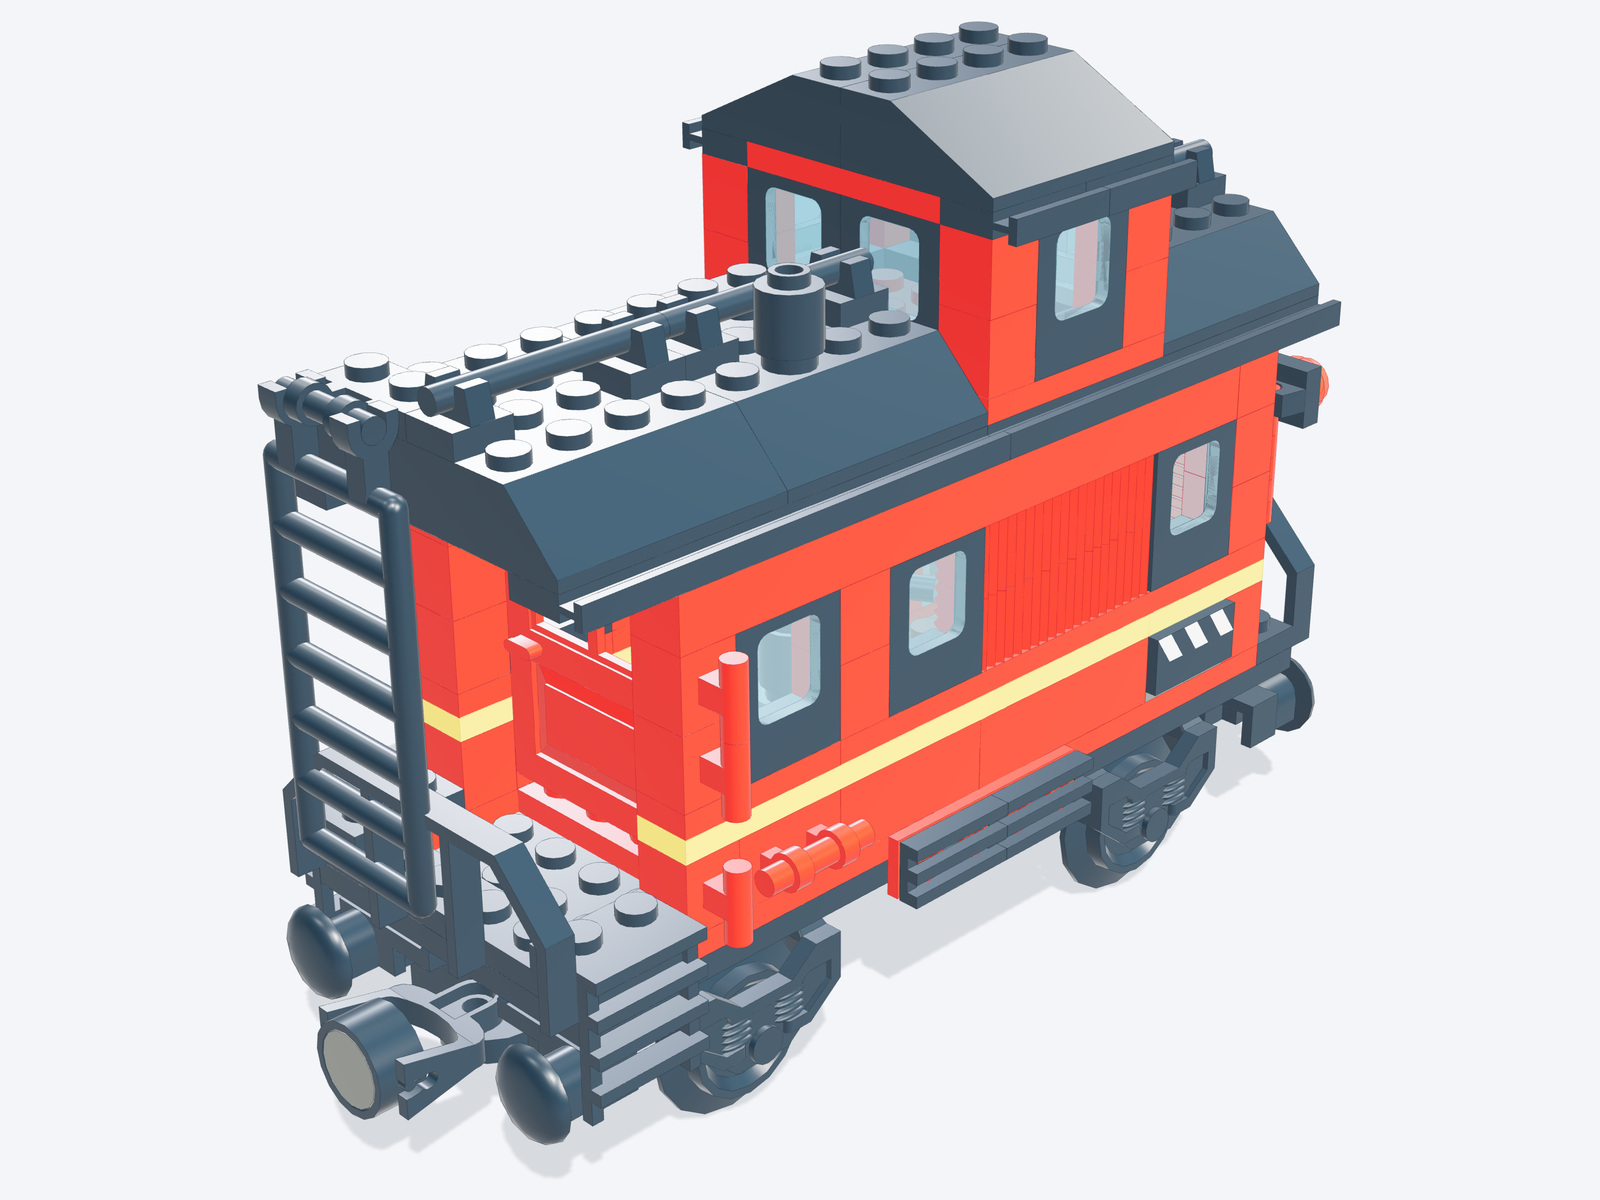
\includegraphics[width=.65\linewidth]{figures-v2/10014-iso.jpg}\end{center}
\paragraph{Attribution.}TotalyWicked [TotalyWicked], OMR by Robert Paciorek [bercik]. CC BY 2.0.\par\url{https://library.ldraw.org/omr/sets/1415}
\paragraph{Source SHA256.}\path{f3aead9fe55512171565803f187f3f7a952fb70515983c39970cffd89431644d}
\paragraph{Connector records.}stud: 440; axle: 10; hinge: 0; fixed: 0; ball: 0
\paragraph{Public input lock.}\path{c22c7968e5b12e1190e57801d20a8ae842ea5a797bf07e78548274307c6b5b65}
\paragraph{Status.}Source preservation does not certify stability. Reference outputs below are internal review material. Full model inputs are the versioned public JSON and numbered PNGs.
\begin{enumerate}
\item \textbf{ld2-10014-color-1}. Identify the original color of B0093; numbered isolation is allowed.
\par{\small color; visual; atomic; single-choice.\par\textit{Operands:} B0093 = brick\_000093\par\textit{Public evidence summary:} Numbered PNG: benchmark/ldraw-v2/inputs/views/ld2-10014-color-1.png; structured input = \{\}.\par\textit{Options:} A: Black; B: Brown; C: Dark Grey; D: Light Grey\par\textit{Reference output:} \{"choiceId": "C"\}\par\textit{Derivation:} source colorName by rendered B-label; source oracle only\par\textit{Equivalence:} exact declared response\par\textit{Review:} pending required human review.}
\item \textbf{ld2-10014-shape-match-1}. Ignoring color and pose, which numbered instance has the same LDraw part type as B0093?
\par{\small shape-match; visual; atomic; single-choice.\par\textit{Operands:} B0004 = brick\_000004, B0093 = brick\_000093, B0002 = brick\_000002, B0094 = brick\_000094, B0114 = brick\_000114\par\textit{Public evidence summary:} Numbered PNG: benchmark/ldraw-v2/inputs/views/ld2-10014-shape-match-1.png; structured input = \{\}.\par\textit{Options:} A: B0004; B: B0114; C: B0094; D: B0002\par\textit{Reference output:} \{"choiceId": "C"\}\par\textit{Derivation:} source partNumber equality across labeled candidates; source oracle only\par\textit{Equivalence:} same source partNumber; ignore color and pose; perceptual equivalence pending\par\textit{Review:} pending required human review.}
\item \textbf{ld2-10014-distance-1}. Using the supplied geometry bounding-box centers, which candidate is nearest to B0093?
\par{\small distance; source-data; atomic; single-choice.\par\textit{Operands:} B0127 = brick\_000127, B0093 = brick\_000093, B0004 = brick\_000004, B0071 = brick\_000071\par\textit{Public evidence summary:} \{"coordinateFrame": "Viewer world, millimeters, Euclidean distance", "centers": \{"B0093": [-4, 2.4, 4], "B0127": [62, 9.6, 0], "B0071": [-12, 18.4, 8], "B0004": [-20, 34.4, -20]\}\}\par\textit{Options:} A: B0004; B: B0127; C: B0071\par\textit{Reference output:} \{"choiceId": "C"\}\par\textit{Derivation:} Euclidean norm from public rounded centers\par\textit{Equivalence:} exact declared response\par\textit{Review:} machine checks passed; no human certification.}
\item \textbf{ld2-10014-color-2}. Identify the original color of B0139; numbered isolation is allowed.
\par{\small color; visual; atomic; single-choice.\par\textit{Operands:} B0139 = brick\_000139\par\textit{Public evidence summary:} Numbered PNG: benchmark/ldraw-v2/inputs/views/ld2-10014-color-2.png; structured input = \{\}.\par\textit{Options:} A: Red; B: Black; C: Yellow; D: Trans Red\par\textit{Reference output:} \{"choiceId": "B"\}\par\textit{Derivation:} source colorName by rendered B-label; source oracle only\par\textit{Equivalence:} exact declared response\par\textit{Review:} pending required human review.}
\item \textbf{ld2-10014-shape-match-2}. Ignoring color and pose, which numbered instance has the same LDraw part type as B0139?
\par{\small shape-match; visual; atomic; single-choice.\par\textit{Operands:} B0078 = brick\_000078, B0165 = brick\_000165, B0139 = brick\_000139, B0134 = brick\_000134, B0137 = brick\_000137\par\textit{Public evidence summary:} Numbered PNG: benchmark/ldraw-v2/inputs/views/ld2-10014-shape-match-2.png; structured input = \{\}.\par\textit{Options:} A: B0165; B: B0137; C: B0134; D: B0078\par\textit{Reference output:} \{"choiceId": "B"\}\par\textit{Derivation:} source partNumber equality across labeled candidates; source oracle only\par\textit{Equivalence:} same source partNumber; ignore color and pose; perceptual equivalence pending\par\textit{Review:} pending required human review.}
\item \textbf{ld2-10014-distance-2}. Using the supplied geometry bounding-box centers, which candidate is nearest to B0139?
\par{\small distance; source-data; atomic; single-choice.\par\textit{Operands:} B0056 = brick\_000056, B0129 = brick\_000129, B0139 = brick\_000139, B0141 = brick\_000141\par\textit{Public evidence summary:} \{"coordinateFrame": "Viewer world, millimeters, Euclidean distance", "centers": \{"B0139": [-20, 44, 12], "B0129": [-8.008, -0.8, -27.2], "B0056": [54.8, 24.8, 20], "B0141": [24, 34.4, 20]\}\}\par\textit{Options:} A: B0141; B: B0056; C: B0129\par\textit{Reference output:} \{"choiceId": "A"\}\par\textit{Derivation:} Euclidean norm from public rounded centers\par\textit{Equivalence:} exact declared response\par\textit{Review:} machine checks passed; no human certification.}
\item \textbf{ld2-10014-interface-1}. Classify the supplied connector record for B0021 and B0019. This does not certify load capacity.
\par{\small interface; connector-graph; metacognitive; single-choice.\par\textit{Operands:} B0019 = brick\_000019, B0021 = brick\_000021\par\textit{Public evidence summary:} \{"connectorRecord": \{"family": "axle", "aConnector": 0, "bConnector": 0\}, "scope": "Upstream connector tolerances and inset mesh intersections; unknown parts remain explicit, separate scene objects are not glued together; no load/force validation."\}\par\textit{Options:} A: fixed; B: axle; C: ball; D: stud; E: hinge\par\textit{Reference output:} \{"choiceId": "B"\}\par\textit{Derivation:} public connectorRecord.family equality\par\textit{Equivalence:} exact declared response\par\textit{Review:} machine checks passed; no human certification.}
\item \textbf{ld2-10014-interface-2}. Classify the supplied connector record for B0082 and B0067. This does not certify load capacity.
\par{\small interface; connector-graph; metacognitive; single-choice.\par\textit{Operands:} B0067 = brick\_000067, B0082 = brick\_000082\par\textit{Public evidence summary:} \{"connectorRecord": \{"family": "stud", "aConnector": 5, "bConnector": 9\}, "scope": "Upstream connector tolerances and inset mesh intersections; unknown parts remain explicit, separate scene objects are not glued together; no load/force validation."\}\par\textit{Options:} A: axle; B: fixed; C: hinge; D: stud; E: ball\par\textit{Reference output:} \{"choiceId": "D"\}\par\textit{Derivation:} public connectorRecord.family equality\par\textit{Equivalence:} exact declared response\par\textit{Review:} machine checks passed; no human certification.}
\item \textbf{ld2-10014-neighbors-1}. Select every candidate directly adjacent to B0032 in the supplied connector graph.
\par{\small neighbors; connector-graph; metacognitive; multiple-choice.\par\textit{Operands:} B0015 = brick\_000015, B0068 = brick\_000068, B0021 = brick\_000021, B0163 = brick\_000163, B0020 = brick\_000020, B0032 = brick\_000032, B0165 = brick\_000165, B0006 = brick\_000006\par\textit{Public evidence summary:} 5 unique undirected pairs\par\textit{Options:} A: B0015; B: B0163; C: B0021; D: B0165; E: B0020; F: B0006; G: B0068\par\textit{Reference output:} \{"choiceIds": ["A", "B", "C", "D", "E"]\}\par\textit{Derivation:} public incident edge endpoint set\par\textit{Equivalence:} unordered exact set; duplicate IDs invalid\par\textit{Review:} machine checks passed; no human certification.}
\item \textbf{ld2-10014-graph-removal-1}. Delete B0032 and its incident edges from this local graph. How many connected components remain? Do not infer physical extractability.
\par{\small graph-removal; connector-graph; graph-internal; integer.\par\textit{Operands:} B0032 = brick\_000032, B0020 = brick\_000020, B0163 = brick\_000163, B0068 = brick\_000068, B0006 = brick\_000006, B0165 = brick\_000165, B0021 = brick\_000021, B0015 = brick\_000015\par\textit{Public evidence summary:} 5 unique undirected pairs; 8 nodes\par\textit{Reference output:} \{"value": 7\}\par\textit{Derivation:} union-find component count after public target deletion\par\textit{Equivalence:} exact declared response\par\textit{Review:} machine checks passed; no human certification.}
\item \textbf{ld2-10014-neighbors-2}. Select every candidate directly adjacent to B0024 in the supplied connector graph.
\par{\small neighbors; connector-graph; metacognitive; multiple-choice.\par\textit{Operands:} B0025 = brick\_000025, B0024 = brick\_000024, B0029 = brick\_000029, B0126 = brick\_000126, B0030 = brick\_000030, B0129 = brick\_000129, B0026 = brick\_000026\par\textit{Public evidence summary:} 4 unique undirected pairs\par\textit{Options:} A: B0025; B: B0129; C: B0029; D: B0030; E: B0026; F: B0126\par\textit{Reference output:} \{"choiceIds": ["A", "C", "D", "E"]\}\par\textit{Derivation:} public incident edge endpoint set\par\textit{Equivalence:} unordered exact set; duplicate IDs invalid\par\textit{Review:} pending required human review.}
\item \textbf{ld2-10014-graph-removal-2}. Delete B0024 and its incident edges from this local graph. How many connected components remain? Do not infer physical extractability.
\par{\small graph-removal; connector-graph; graph-internal; integer.\par\textit{Operands:} B0024 = brick\_000024, B0026 = brick\_000026, B0025 = brick\_000025, B0129 = brick\_000129, B0029 = brick\_000029, B0030 = brick\_000030, B0126 = brick\_000126\par\textit{Public evidence summary:} 4 unique undirected pairs; 7 nodes\par\textit{Reference output:} \{"value": 6\}\par\textit{Derivation:} union-find component count after public target deletion\par\textit{Equivalence:} exact declared response\par\textit{Review:} pending required human review.}
\item \textbf{ld2-10014-coverage-1}. Which numbered instance lacks a connector definition in the coverage record, so this audit cannot establish that it is floating?
\par{\small coverage; source-data; metacognitive; single-choice.\par\textit{Operands:} B0093 = brick\_000093, B0139 = brick\_000139, B0074 = brick\_000074, B0033 = brick\_000033\par\textit{Public evidence summary:} \{"coverage": [\{"label": "B0033", "supported": false\}, \{"label": "B0074", "supported": true\}, \{"label": "B0139", "supported": true\}, \{"label": "B0093", "supported": true\}]\}\par\textit{Options:} A: B0074; B: B0033; C: B0139; D: B0093\par\textit{Reference output:} \{"choiceId": "B"\}\par\textit{Derivation:} public supported=false record\par\textit{Equivalence:} exact declared response\par\textit{Review:} pending required human review.}
\item \textbf{ld2-10014-evidence-limit-1}. Only source geometry, connector matching and mesh intersection audits are available. Without mass, friction, material or dynamic tests, is gravitational stability established?
\par{\small evidence-limit; source-data; metacognitive; single-choice.\par\textit{Operands:} none\par\textit{Public evidence summary:} \{"available": ["Original CAD", "Connector inference", "Inset-mesh intersection candidates"]\}\par\textit{Options:} A: Established; B: Not established by this evidence\par\textit{Reference output:} \{"choiceId": "B"\}\par\textit{Derivation:} fixed epistemic control label\par\textit{Equivalence:} exact declared response\par\textit{Review:} machine checks passed; no human certification.}
\item \textbf{ld2-10014-restore-instance-1}. The display copy hides B0093. Restore only that numbered instance, preserving all other instances and source poses.
\par{\small restore-instance; scene-edit; procedural; actions.\par\textit{Operands:} B0093 = brick\_000093, B0001 = brick\_000001\par\textit{Public evidence summary:} 2 public actions; budget 1; \{"initialFacts": ["missing-brick\_000093", "present-brick\_000001"], "goalFacts": ["present-brick\_000093", "present-brick\_000001"], "absentFacts": ["missing-brick\_000093"]\}\par\textit{Reference output:} \{"actionIds": ["restore-B0093"]\}\par\textit{Derivation:} public precondition solver\par\textit{Equivalence:} any legal sequence reaching all goals within budget; display-only semantics\par\textit{Review:} machine checks passed; no human certification.}
\item \textbf{ld2-10014-restore-instance-2}. The display copy hides B0139. Restore only that numbered instance, preserving all other instances and source poses.
\par{\small restore-instance; scene-edit; procedural; actions.\par\textit{Operands:} B0139 = brick\_000139, B0001 = brick\_000001\par\textit{Public evidence summary:} 2 public actions; budget 1; \{"initialFacts": ["missing-brick\_000139", "present-brick\_000001"], "goalFacts": ["present-brick\_000139", "present-brick\_000001"], "absentFacts": ["missing-brick\_000139"]\}\par\textit{Reference output:} \{"actionIds": ["restore-B0139"]\}\par\textit{Derivation:} public precondition solver\par\textit{Equivalence:} any legal sequence reaching all goals within budget; display-only semantics\par\textit{Review:} machine checks passed; no human certification.}
\end{enumerate}
\clearpage\section{31031: Rainforest Animals}
215 source instances; 20 tasks; D2 size band. 61 type strings; 15 color codes; 0 unsupported instances; 7 intersection candidates. 130 expanded author steps. Independent reparse: passed.
\begin{center}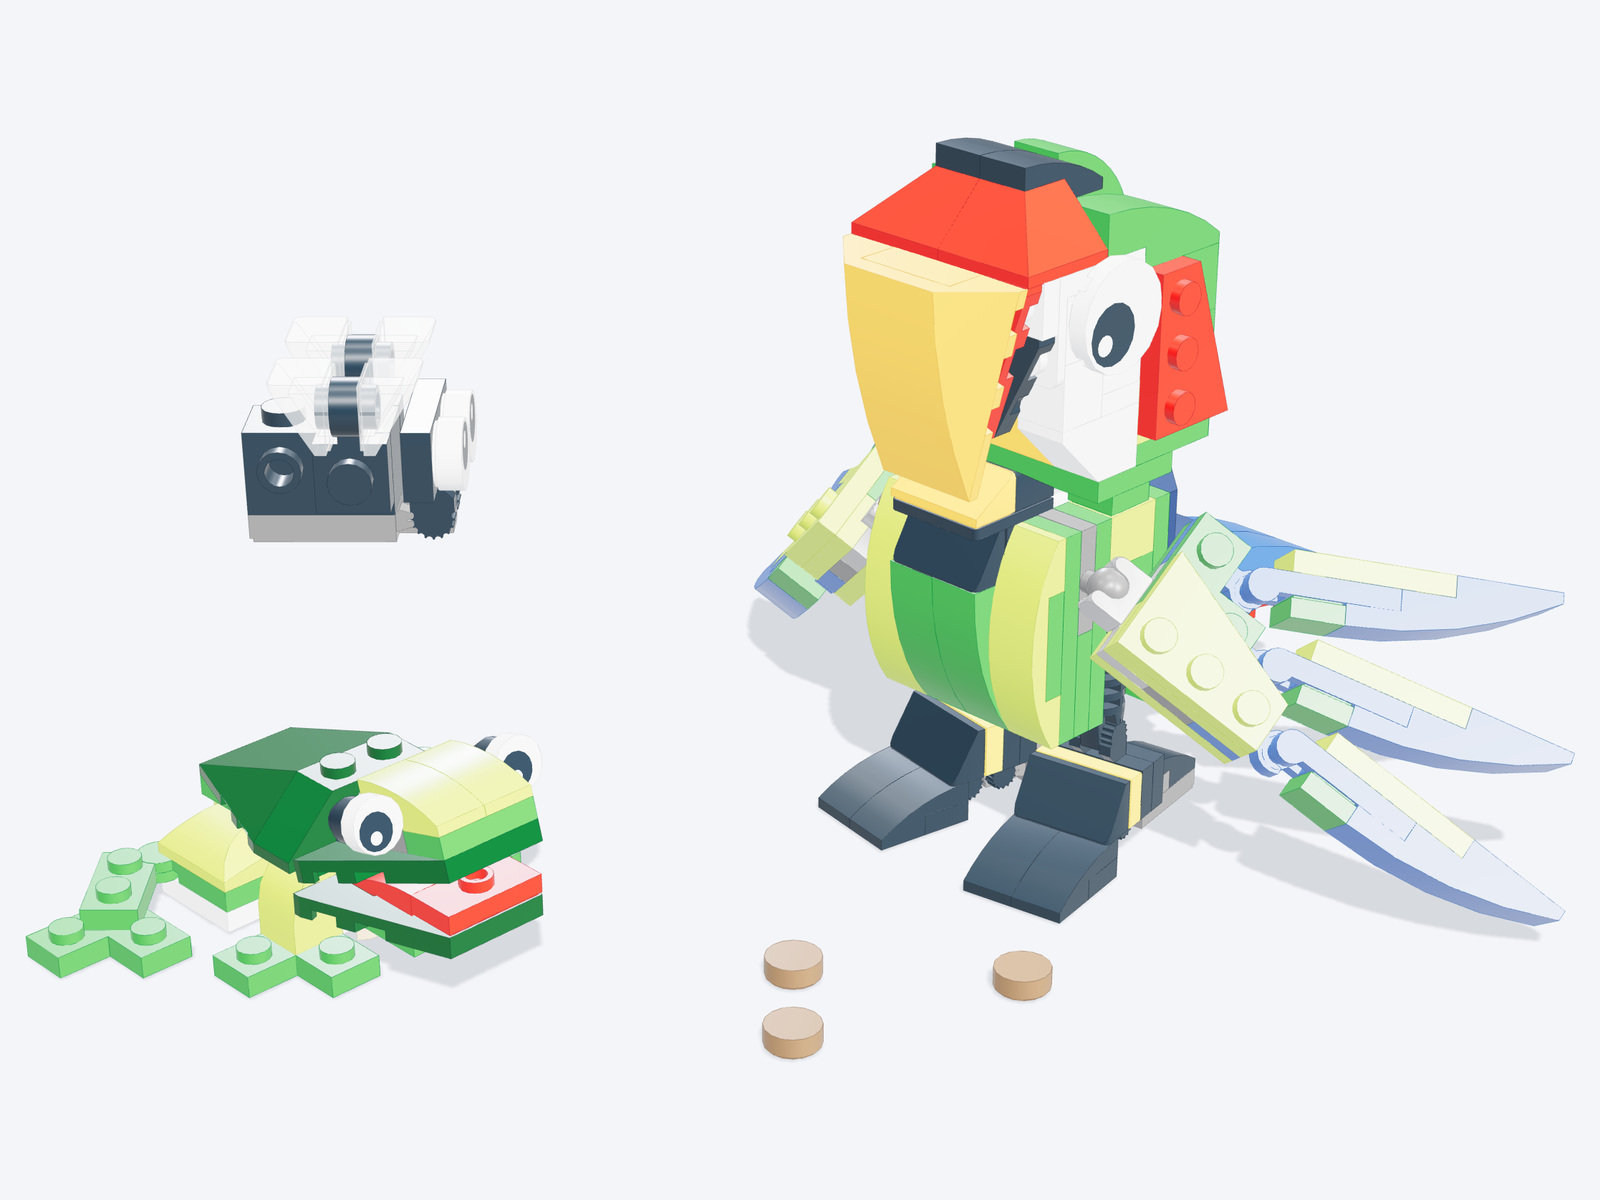
\includegraphics[width=.65\linewidth]{figures-v2/omr-31031-iso.jpg}\end{center}
\paragraph{Attribution.}Marc Giraudet [Mad\_Marc]. CC BY 2.0.\par\url{https://library.ldraw.org/library/omr/31031-1.mpd}
\paragraph{Source SHA256.}\path{b5b87230d2fe147aa1135baee5d1604a283f1e586a228b27b351253af5565da7}
\paragraph{Connector records.}stud: 396; axle: 8; hinge: 9; fixed: 0; ball: 3
\paragraph{Public input lock.}\path{2398c12a777d407e5e3d76cccc9e2bd313c0aaa70f039215d7fac29d609b2562}
\paragraph{Status.}Source preservation does not certify stability. Reference outputs below are internal review material. Full model inputs are the versioned public JSON and numbered PNGs.
\begin{enumerate}
\item \textbf{ld2-omr-31031-color-1}. Identify the original color of B0182; numbered isolation is allowed.
\par{\small color; visual; atomic; single-choice.\par\textit{Operands:} B0182 = brick\_000182\par\textit{Public evidence summary:} Numbered PNG: benchmark/ldraw-v2/inputs/views/ld2-omr-31031-color-1.png; structured input = \{\}.\par\textit{Options:} A: Trans Clear; B: Green; C: Bright Light Orange; D: Blue\par\textit{Reference output:} \{"choiceId": "B"\}\par\textit{Derivation:} source colorName by rendered B-label; source oracle only\par\textit{Equivalence:} exact declared response\par\textit{Review:} pending required human review.}
\item \textbf{ld2-omr-31031-shape-match-1}. Ignoring color and pose, which numbered instance has the same LDraw part type as B0182?
\par{\small shape-match; visual; atomic; single-choice.\par\textit{Operands:} B0063 = brick\_000063, B0177 = brick\_000177, B0182 = brick\_000182, B0118 = brick\_000118, B0071 = brick\_000071\par\textit{Public evidence summary:} Numbered PNG: benchmark/ldraw-v2/inputs/views/ld2-omr-31031-shape-match-1.png; structured input = \{\}.\par\textit{Options:} A: B0071; B: B0177; C: B0118; D: B0063\par\textit{Reference output:} \{"choiceId": "B"\}\par\textit{Derivation:} source partNumber equality across labeled candidates; source oracle only\par\textit{Equivalence:} same source partNumber; ignore color and pose; perceptual equivalence pending\par\textit{Review:} pending required human review.}
\item \textbf{ld2-omr-31031-distance-1}. Using the supplied geometry bounding-box centers, which candidate is nearest to B0182?
\par{\small distance; source-data; atomic; single-choice.\par\textit{Operands:} B0004 = brick\_000004, B0096 = brick\_000096, B0038 = brick\_000038, B0182 = brick\_000182\par\textit{Public evidence summary:} \{"coordinateFrame": "Viewer world, millimeters, Euclidean distance", "centers": \{"B0182": [11.8912, 42.1888, -13.4232], "B0038": [-80, 22.103829, -19.584571], "B0096": [-6.066, 3.200012, 2.0992], "B0004": [-115.958788, 106.4, 14.991612]\}\}\par\textit{Options:} A: B0096; B: B0004; C: B0038\par\textit{Reference output:} \{"choiceId": "A"\}\par\textit{Derivation:} Euclidean norm from public rounded centers\par\textit{Equivalence:} exact declared response\par\textit{Review:} machine checks passed; no human certification.}
\item \textbf{ld2-omr-31031-color-2}. Identify the original color of B0111; numbered isolation is allowed.
\par{\small color; visual; atomic; single-choice.\par\textit{Operands:} B0111 = brick\_000111\par\textit{Public evidence summary:} Numbered PNG: benchmark/ldraw-v2/inputs/views/ld2-omr-31031-color-2.png; structured input = \{\}.\par\textit{Options:} A: Green; B: Yellow; C: Lime; D: White\par\textit{Reference output:} \{"choiceId": "A"\}\par\textit{Derivation:} source colorName by rendered B-label; source oracle only\par\textit{Equivalence:} exact declared response\par\textit{Review:} pending required human review.}
\item \textbf{ld2-omr-31031-shape-match-2}. Ignoring color and pose, which numbered instance has the same LDraw part type as B0111?
\par{\small shape-match; visual; atomic; single-choice.\par\textit{Operands:} B0097 = brick\_000097, B0141 = brick\_000141, B0111 = brick\_000111, B0005 = brick\_000005, B0098 = brick\_000098\par\textit{Public evidence summary:} Numbered PNG: benchmark/ldraw-v2/inputs/views/ld2-omr-31031-shape-match-2.png; structured input = \{\}.\par\textit{Options:} A: B0141; B: B0005; C: B0098; D: B0097\par\textit{Reference output:} \{"choiceId": "A"\}\par\textit{Derivation:} source partNumber equality across labeled candidates; source oracle only\par\textit{Equivalence:} same source partNumber; ignore color and pose; perceptual equivalence pending\par\textit{Review:} pending required human review.}
\item \textbf{ld2-omr-31031-distance-2}. Using the supplied geometry bounding-box centers, which candidate is nearest to B0111?
\par{\small distance; source-data; atomic; single-choice.\par\textit{Operands:} B0094 = brick\_000094, B0111 = brick\_000111, B0142 = brick\_000142, B0149 = brick\_000149\par\textit{Public evidence summary:} \{"coordinateFrame": "Viewer world, millimeters, Euclidean distance", "centers": \{"B0111": [14.4, 69.6, 12.8], "B0142": [14.4, 92.8, 8.8], "B0094": [1.3218, 2.4, -1.1448], "B0149": [2.4, 85.6, 30.4]\}\}\par\textit{Options:} A: B0094; B: B0142; C: B0149\par\textit{Reference output:} \{"choiceId": "B"\}\par\textit{Derivation:} Euclidean norm from public rounded centers\par\textit{Equivalence:} exact declared response\par\textit{Review:} machine checks passed; no human certification.}
\item \textbf{ld2-omr-31031-interface-1}. Classify the supplied connector record for B0049 and B0110. This does not certify load capacity.
\par{\small interface; connector-graph; metacognitive; single-choice.\par\textit{Operands:} B0049 = brick\_000049, B0110 = brick\_000110\par\textit{Public evidence summary:} \{"connectorRecord": \{"family": "axle", "aConnector": 1, "bConnector": 0\}, "scope": "Upstream connector tolerances and inset mesh intersections; unknown parts remain explicit, separate scene objects are not glued together; no load/force validation."\}\par\textit{Options:} A: hinge; B: fixed; C: axle; D: ball; E: stud\par\textit{Reference output:} \{"choiceId": "C"\}\par\textit{Derivation:} public connectorRecord.family equality\par\textit{Equivalence:} exact declared response\par\textit{Review:} machine checks passed; no human certification.}
\item \textbf{ld2-omr-31031-interface-2}. Classify the supplied connector record for B0038 and B0035. This does not certify load capacity.
\par{\small interface; connector-graph; metacognitive; single-choice.\par\textit{Operands:} B0038 = brick\_000038, B0035 = brick\_000035\par\textit{Public evidence summary:} \{"connectorRecord": \{"family": "ball", "aConnector": 3, "bConnector": 3\}, "scope": "Upstream connector tolerances and inset mesh intersections; unknown parts remain explicit, separate scene objects are not glued together; no load/force validation."\}\par\textit{Options:} A: axle; B: fixed; C: hinge; D: stud; E: ball\par\textit{Reference output:} \{"choiceId": "E"\}\par\textit{Derivation:} public connectorRecord.family equality\par\textit{Equivalence:} exact declared response\par\textit{Review:} machine checks passed; no human certification.}
\item \textbf{ld2-omr-31031-interface-3}. Classify the supplied connector record for B0015 and B0016. This does not certify load capacity.
\par{\small interface; connector-graph; metacognitive; single-choice.\par\textit{Operands:} B0015 = brick\_000015, B0016 = brick\_000016\par\textit{Public evidence summary:} \{"connectorRecord": \{"family": "hinge", "aConnector": 1, "bConnector": 2\}, "scope": "Upstream connector tolerances and inset mesh intersections; unknown parts remain explicit, separate scene objects are not glued together; no load/force validation."\}\par\textit{Options:} A: stud; B: fixed; C: axle; D: ball; E: hinge\par\textit{Reference output:} \{"choiceId": "E"\}\par\textit{Derivation:} public connectorRecord.family equality\par\textit{Equivalence:} exact declared response\par\textit{Review:} machine checks passed; no human certification.}
\item \textbf{ld2-omr-31031-interface-4}. Classify the supplied connector record for B0126 and B0134. This does not certify load capacity.
\par{\small interface; connector-graph; metacognitive; single-choice.\par\textit{Operands:} B0126 = brick\_000126, B0134 = brick\_000134\par\textit{Public evidence summary:} \{"connectorRecord": \{"family": "stud", "aConnector": 11, "bConnector": 3\}, "scope": "Upstream connector tolerances and inset mesh intersections; unknown parts remain explicit, separate scene objects are not glued together; no load/force validation."\}\par\textit{Options:} A: hinge; B: stud; C: ball; D: fixed; E: axle\par\textit{Reference output:} \{"choiceId": "B"\}\par\textit{Derivation:} public connectorRecord.family equality\par\textit{Equivalence:} exact declared response\par\textit{Review:} machine checks passed; no human certification.}
\item \textbf{ld2-omr-31031-neighbors-1}. Select every candidate directly adjacent to B0131 in the supplied connector graph.
\par{\small neighbors; connector-graph; metacognitive; multiple-choice.\par\textit{Operands:} B0144 = brick\_000144, B0163 = brick\_000163, B0124 = brick\_000124, B0132 = brick\_000132, B0131 = brick\_000131, B0020 = brick\_000020\par\textit{Public evidence summary:} 3 unique undirected pairs\par\textit{Options:} A: B0144; B: B0124; C: B0163; D: B0020; E: B0132\par\textit{Reference output:} \{"choiceIds": ["A", "B", "E"]\}\par\textit{Derivation:} public incident edge endpoint set\par\textit{Equivalence:} unordered exact set; duplicate IDs invalid\par\textit{Review:} pending required human review.}
\item \textbf{ld2-omr-31031-graph-removal-1}. Delete B0131 and its incident edges from this local graph. How many connected components remain? Do not infer physical extractability.
\par{\small graph-removal; connector-graph; graph-internal; integer.\par\textit{Operands:} B0124 = brick\_000124, B0131 = brick\_000131, B0144 = brick\_000144, B0163 = brick\_000163, B0020 = brick\_000020, B0132 = brick\_000132\par\textit{Public evidence summary:} 3 unique undirected pairs; 6 nodes\par\textit{Reference output:} \{"value": 5\}\par\textit{Derivation:} union-find component count after public target deletion\par\textit{Equivalence:} exact declared response\par\textit{Review:} pending required human review.}
\item \textbf{ld2-omr-31031-neighbors-2}. Select every candidate directly adjacent to B0166 in the supplied connector graph.
\par{\small neighbors; connector-graph; metacognitive; multiple-choice.\par\textit{Operands:} B0166 = brick\_000166, B0165 = brick\_000165, B0202 = brick\_000202, B0162 = brick\_000162, B0094 = brick\_000094\par\textit{Public evidence summary:} 3 unique undirected pairs\par\textit{Options:} A: B0202; B: B0094; C: B0162; D: B0165\par\textit{Reference output:} \{"choiceIds": ["C", "D"]\}\par\textit{Derivation:} public incident edge endpoint set\par\textit{Equivalence:} unordered exact set; duplicate IDs invalid\par\textit{Review:} pending required human review.}
\item \textbf{ld2-omr-31031-graph-removal-2}. Delete B0166 and its incident edges from this local graph. How many connected components remain? Do not infer physical extractability.
\par{\small graph-removal; connector-graph; graph-internal; integer.\par\textit{Operands:} B0165 = brick\_000165, B0162 = brick\_000162, B0094 = brick\_000094, B0202 = brick\_000202, B0166 = brick\_000166\par\textit{Public evidence summary:} 3 unique undirected pairs; 5 nodes\par\textit{Reference output:} \{"value": 3\}\par\textit{Derivation:} union-find component count after public target deletion\par\textit{Equivalence:} exact declared response\par\textit{Review:} pending required human review.}
\item \textbf{ld2-omr-31031-evidence-limit-1}. Only source geometry, connector matching and mesh intersection audits are available. Without mass, friction, material or dynamic tests, is gravitational stability established?
\par{\small evidence-limit; source-data; metacognitive; single-choice.\par\textit{Operands:} none\par\textit{Public evidence summary:} \{"available": ["Original CAD", "Connector inference", "Inset-mesh intersection candidates"]\}\par\textit{Options:} A: Not established by this evidence; B: Established\par\textit{Reference output:} \{"choiceId": "A"\}\par\textit{Derivation:} fixed epistemic control label\par\textit{Equivalence:} exact declared response\par\textit{Review:} machine checks passed; no human certification.}
\item \textbf{ld2-omr-31031-source-step-1}. At which expanded author step does B0082 first appear in the supplied source-step table? Source order is not a collision-free assembly proof.
\par{\small source-step; source-data; procedural; single-choice.\par\textit{Operands:} B0001 = brick\_000001, B0082 = brick\_000082\par\textit{Public evidence summary:} 2 supplied author-step records; exact table in public JSON\par\textit{Options:} A: 9; B: 28; C: 45; D: 24\par\textit{Reference output:} \{"choiceId": "C"\}\par\textit{Derivation:} minimum public step index containing target\par\textit{Equivalence:} exact declared response\par\textit{Review:} machine checks passed; no human certification.}
\item \textbf{ld2-omr-31031-source-step-2}. At which expanded author step does B0168 first appear in the supplied source-step table? Source order is not a collision-free assembly proof.
\par{\small source-step; source-data; procedural; single-choice.\par\textit{Operands:} B0001 = brick\_000001, B0168 = brick\_000168\par\textit{Public evidence summary:} 2 supplied author-step records; exact table in public JSON\par\textit{Options:} A: 93; B: 112; C: 4; D: 128\par\textit{Reference output:} \{"choiceId": "A"\}\par\textit{Derivation:} minimum public step index containing target\par\textit{Equivalence:} exact declared response\par\textit{Review:} machine checks passed; no human certification.}
\item \textbf{ld2-omr-31031-source-sequence-1}. Reveal the supplied source-step window in author order. Actions change visibility only, without simulating insertion trajectories.
\par{\small source-sequence; scene-edit; procedural; actions.\par\textit{Operands:} B0006 = brick\_000006, B0002 = brick\_000002, B0004 = brick\_000004, B0005 = brick\_000005, B0007 = brick\_000007, B0001 = brick\_000001, B0009 = brick\_000009, B0003 = brick\_000003, B0008 = brick\_000008\par\textit{Public evidence summary:} 6 public actions; budget 6; \{"initialFacts": ["start"], "goalFacts": ["done-6"], "absentFacts": []\}\par\textit{Reference output:} \{"actionIds": ["step-1", "step-2", "step-3", "step-4", "step-5", "step-6"]\}\par\textit{Derivation:} public precondition solver\par\textit{Equivalence:} any legal sequence reaching all goals within budget; display-only semantics\par\textit{Review:} machine checks passed; no human certification.}
\item \textbf{ld2-omr-31031-restore-instance-1}. The display copy hides B0182. Restore only that numbered instance, preserving all other instances and source poses.
\par{\small restore-instance; scene-edit; procedural; actions.\par\textit{Operands:} B0182 = brick\_000182, B0001 = brick\_000001\par\textit{Public evidence summary:} 2 public actions; budget 1; \{"initialFacts": ["missing-brick\_000182", "present-brick\_000001"], "goalFacts": ["present-brick\_000182", "present-brick\_000001"], "absentFacts": ["missing-brick\_000182"]\}\par\textit{Reference output:} \{"actionIds": ["restore-B0182"]\}\par\textit{Derivation:} public precondition solver\par\textit{Equivalence:} any legal sequence reaching all goals within budget; display-only semantics\par\textit{Review:} machine checks passed; no human certification.}
\item \textbf{ld2-omr-31031-restore-instance-2}. The display copy hides B0111. Restore only that numbered instance, preserving all other instances and source poses.
\par{\small restore-instance; scene-edit; procedural; actions.\par\textit{Operands:} B0001 = brick\_000001, B0111 = brick\_000111\par\textit{Public evidence summary:} 2 public actions; budget 1; \{"initialFacts": ["missing-brick\_000111", "present-brick\_000001"], "goalFacts": ["present-brick\_000111", "present-brick\_000001"], "absentFacts": ["missing-brick\_000111"]\}\par\textit{Reference output:} \{"actionIds": ["restore-B0111"]\}\par\textit{Derivation:} public precondition solver\par\textit{Equivalence:} any legal sequence reaching all goals within budget; display-only semantics\par\textit{Review:} machine checks passed; no human certification.}
\end{enumerate}
\clearpage\section{31088: Deep Sea Creatures}
230 source instances; 20 tasks; D2 size band. 71 type strings; 12 color codes; 4 unsupported instances; 4 intersection candidates. 98 expanded author steps. Independent reparse: passed.
\begin{center}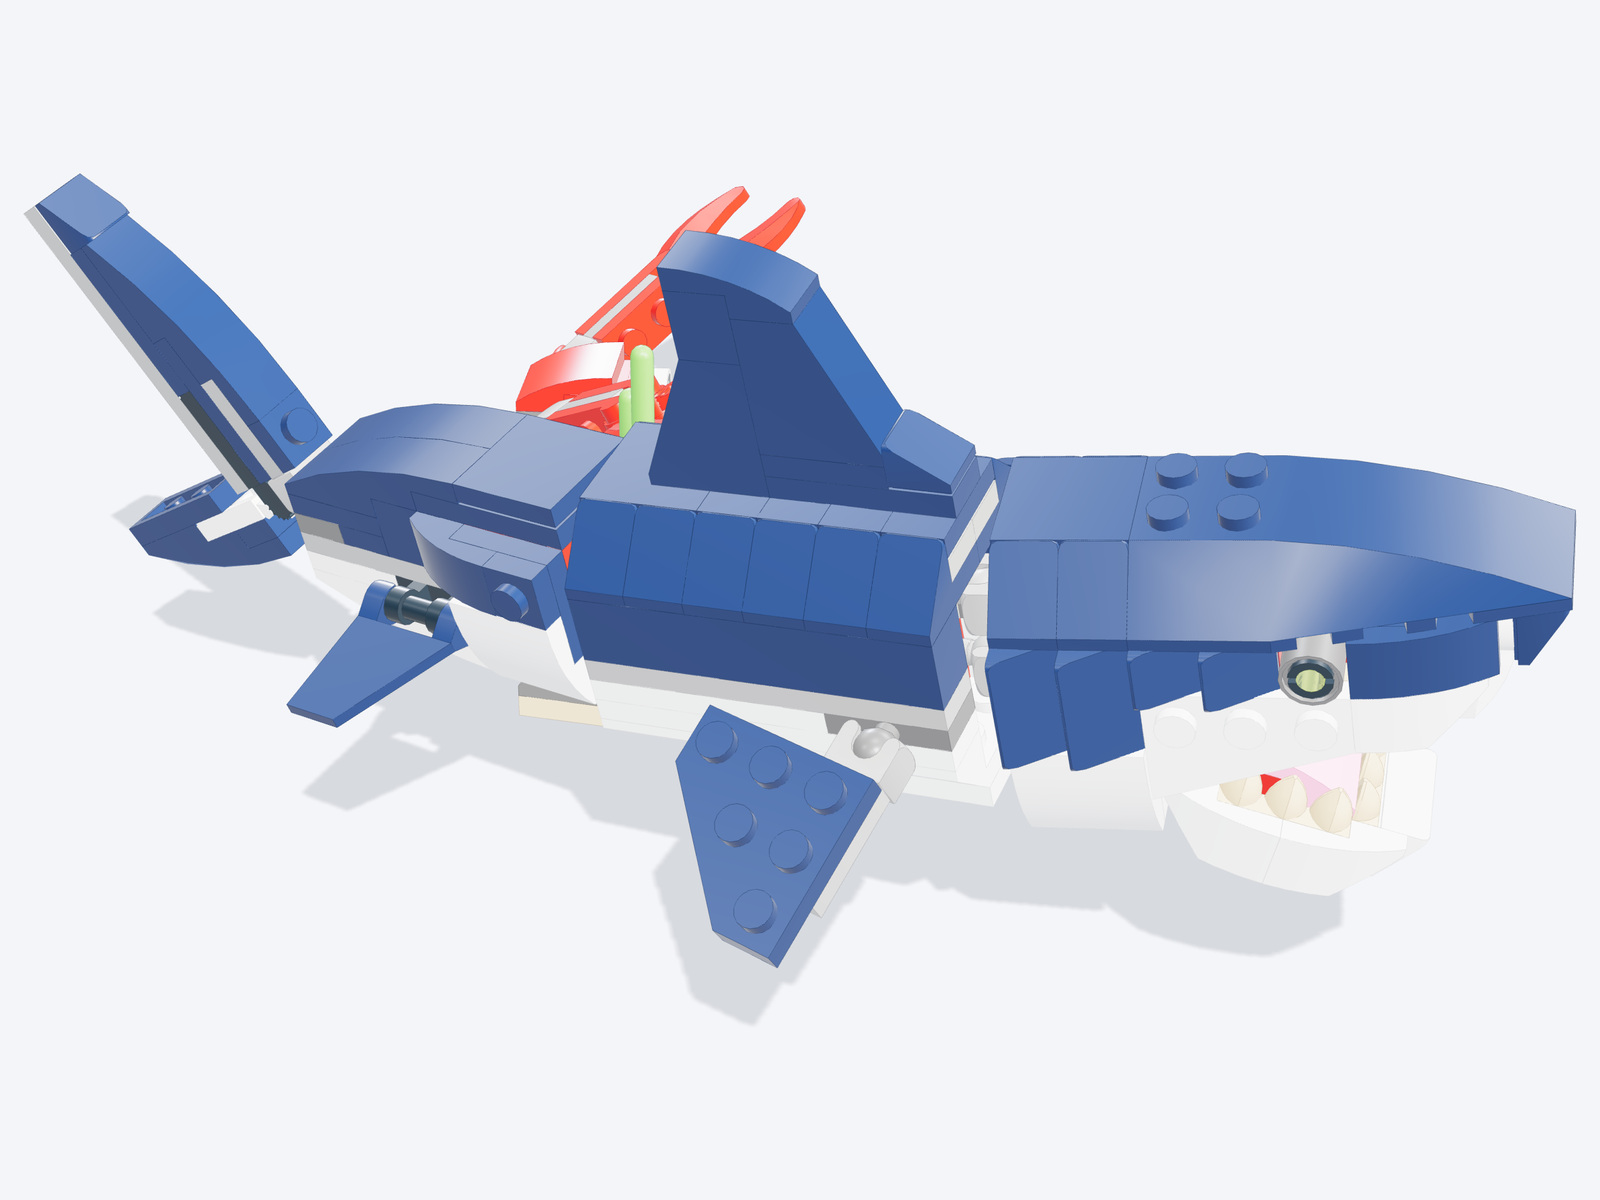
\includegraphics[width=.65\linewidth]{figures-v2/omr-31088-iso.jpg}\end{center}
\paragraph{Attribution.}Marc Belanger [MonsieurPoulet]. CC BY 2.0.\par\url{https://library.ldraw.org/library/omr/31088-1.mpd}
\paragraph{Source SHA256.}\path{c5cc0f95664d50244295783163d1ba3c73484f4b9bbfca89ada8bb1de0dbfff5}
\paragraph{Connector records.}stud: 440; axle: 29; hinge: 2; fixed: 0; ball: 4
\paragraph{Public input lock.}\path{efb16992b05a5995159dd2148b6940c1bf6dc841eda128c442e2fbf037e121fd}
\paragraph{Status.}Source preservation does not certify stability. Reference outputs below are internal review material. Full model inputs are the versioned public JSON and numbered PNGs.
\begin{enumerate}
\item \textbf{ld2-omr-31088-color-1}. Identify the original color of B0176; numbered isolation is allowed.
\par{\small color; visual; atomic; single-choice.\par\textit{Operands:} B0176 = brick\_000176\par\textit{Public evidence summary:} Numbered PNG: benchmark/ldraw-v2/inputs/views/ld2-omr-31088-color-1.png; structured input = \{\}.\par\textit{Options:} A: Pearl Gold; B: Dark Blue; C: Red; D: Bright Pink\par\textit{Reference output:} \{"choiceId": "B"\}\par\textit{Derivation:} source colorName by rendered B-label; source oracle only\par\textit{Equivalence:} exact declared response\par\textit{Review:} pending required human review.}
\item \textbf{ld2-omr-31088-shape-match-1}. Ignoring color and pose, which numbered instance has the same LDraw part type as B0176?
\par{\small shape-match; visual; atomic; single-choice.\par\textit{Operands:} B0203 = brick\_000203, B0176 = brick\_000176, B0173 = brick\_000173, B0158 = brick\_000158, B0127 = brick\_000127\par\textit{Public evidence summary:} Numbered PNG: benchmark/ldraw-v2/inputs/views/ld2-omr-31088-shape-match-1.png; structured input = \{\}.\par\textit{Options:} A: B0203; B: B0158; C: B0127; D: B0173\par\textit{Reference output:} \{"choiceId": "D"\}\par\textit{Derivation:} source partNumber equality across labeled candidates; source oracle only\par\textit{Equivalence:} same source partNumber; ignore color and pose; perceptual equivalence pending\par\textit{Review:} pending required human review.}
\item \textbf{ld2-omr-31088-distance-1}. Using the supplied geometry bounding-box centers, which candidate is nearest to B0176?
\par{\small distance; source-data; atomic; single-choice.\par\textit{Operands:} B0176 = brick\_000176, B0219 = brick\_000219, B0218 = brick\_000218, B0134 = brick\_000134\par\textit{Public evidence summary:} \{"coordinateFrame": "Viewer world, millimeters, Euclidean distance", "centers": \{"B0176": [-33.556, 26.7832, -46.9752], "B0134": [-22.2252, 26.8516, -9.6216], "B0218": [55.2016, 12, -67.3224], "B0219": [60.4518, 12, -67.413]\}\}\par\textit{Options:} A: B0134; B: B0219; C: B0218\par\textit{Reference output:} \{"choiceId": "A"\}\par\textit{Derivation:} Euclidean norm from public rounded centers\par\textit{Equivalence:} exact declared response\par\textit{Review:} machine checks passed; no human certification.}
\item \textbf{ld2-omr-31088-color-2}. Identify the original color of B0038; numbered isolation is allowed.
\par{\small color; visual; atomic; single-choice.\par\textit{Operands:} B0038 = brick\_000038\par\textit{Public evidence summary:} Numbered PNG: benchmark/ldraw-v2/inputs/views/ld2-omr-31088-color-2.png; structured input = \{\}.\par\textit{Options:} A: Reddish Brown; B: White; C: Trans Neon Green; D: Pearl Gold\par\textit{Reference output:} \{"choiceId": "B"\}\par\textit{Derivation:} source colorName by rendered B-label; source oracle only\par\textit{Equivalence:} exact declared response\par\textit{Review:} pending required human review.}
\item \textbf{ld2-omr-31088-distance-2}. Using the supplied geometry bounding-box centers, which candidate is nearest to B0038?
\par{\small distance; source-data; atomic; single-choice.\par\textit{Operands:} B0038 = brick\_000038, B0063 = brick\_000063, B0170 = brick\_000170, B0189 = brick\_000189\par\textit{Public evidence summary:} \{"coordinateFrame": "Viewer world, millimeters, Euclidean distance", "centers": \{"B0038": [18.2528, 49.856, 114.62], "B0189": [22.964412, 16.89552, 11.27296], "B0170": [-48.90888, 71.1572, -64.25804], "B0063": [24.036997, 55.442263, 103.184794]\}\}\par\textit{Options:} A: B0189; B: B0170; C: B0063\par\textit{Reference output:} \{"choiceId": "C"\}\par\textit{Derivation:} Euclidean norm from public rounded centers\par\textit{Equivalence:} exact declared response\par\textit{Review:} machine checks passed; no human certification.}
\item \textbf{ld2-omr-31088-interface-1}. Classify the supplied connector record for B0210 and B0211. This does not certify load capacity.
\par{\small interface; connector-graph; metacognitive; single-choice.\par\textit{Operands:} B0210 = brick\_000210, B0211 = brick\_000211\par\textit{Public evidence summary:} \{"connectorRecord": \{"family": "axle", "aConnector": 1, "bConnector": 0\}, "scope": "Upstream connector tolerances and inset mesh intersections; unknown parts remain explicit, separate scene objects are not glued together; no load/force validation."\}\par\textit{Options:} A: axle; B: stud; C: hinge; D: fixed; E: ball\par\textit{Reference output:} \{"choiceId": "A"\}\par\textit{Derivation:} public connectorRecord.family equality\par\textit{Equivalence:} exact declared response\par\textit{Review:} machine checks passed; no human certification.}
\item \textbf{ld2-omr-31088-interface-2}. Classify the supplied connector record for B0089 and B0124. This does not certify load capacity.
\par{\small interface; connector-graph; metacognitive; single-choice.\par\textit{Operands:} B0124 = brick\_000124, B0089 = brick\_000089\par\textit{Public evidence summary:} \{"connectorRecord": \{"family": "ball", "aConnector": 3, "bConnector": 3\}, "scope": "Upstream connector tolerances and inset mesh intersections; unknown parts remain explicit, separate scene objects are not glued together; no load/force validation."\}\par\textit{Options:} A: hinge; B: axle; C: ball; D: fixed; E: stud\par\textit{Reference output:} \{"choiceId": "C"\}\par\textit{Derivation:} public connectorRecord.family equality\par\textit{Equivalence:} exact declared response\par\textit{Review:} machine checks passed; no human certification.}
\item \textbf{ld2-omr-31088-interface-3}. Classify the supplied connector record for B0184 and B0180. This does not certify load capacity.
\par{\small interface; connector-graph; metacognitive; single-choice.\par\textit{Operands:} B0180 = brick\_000180, B0184 = brick\_000184\par\textit{Public evidence summary:} \{"connectorRecord": \{"family": "hinge", "aConnector": 6, "bConnector": 2\}, "scope": "Upstream connector tolerances and inset mesh intersections; unknown parts remain explicit, separate scene objects are not glued together; no load/force validation."\}\par\textit{Options:} A: ball; B: axle; C: stud; D: hinge; E: fixed\par\textit{Reference output:} \{"choiceId": "D"\}\par\textit{Derivation:} public connectorRecord.family equality\par\textit{Equivalence:} exact declared response\par\textit{Review:} machine checks passed; no human certification.}
\item \textbf{ld2-omr-31088-interface-4}. Classify the supplied connector record for B0043 and B0044. This does not certify load capacity.
\par{\small interface; connector-graph; metacognitive; single-choice.\par\textit{Operands:} B0043 = brick\_000043, B0044 = brick\_000044\par\textit{Public evidence summary:} \{"connectorRecord": \{"family": "stud", "aConnector": 5, "bConnector": 2\}, "scope": "Upstream connector tolerances and inset mesh intersections; unknown parts remain explicit, separate scene objects are not glued together; no load/force validation."\}\par\textit{Options:} A: ball; B: axle; C: hinge; D: stud; E: fixed\par\textit{Reference output:} \{"choiceId": "D"\}\par\textit{Derivation:} public connectorRecord.family equality\par\textit{Equivalence:} exact declared response\par\textit{Review:} machine checks passed; no human certification.}
\item \textbf{ld2-omr-31088-neighbors-1}. Select every candidate directly adjacent to B0045 in the supplied connector graph.
\par{\small neighbors; connector-graph; metacognitive; multiple-choice.\par\textit{Operands:} B0057 = brick\_000057, B0061 = brick\_000061, B0081 = brick\_000081, B0039 = brick\_000039, B0043 = brick\_000043, B0045 = brick\_000045\par\textit{Public evidence summary:} 4 unique undirected pairs\par\textit{Options:} A: B0057; B: B0061; C: B0043; D: B0081; E: B0039\par\textit{Reference output:} \{"choiceIds": ["A", "B", "C"]\}\par\textit{Derivation:} public incident edge endpoint set\par\textit{Equivalence:} unordered exact set; duplicate IDs invalid\par\textit{Review:} machine checks passed; no human certification.}
\item \textbf{ld2-omr-31088-graph-removal-1}. Delete B0045 and its incident edges from this local graph. How many connected components remain? Do not infer physical extractability.
\par{\small graph-removal; connector-graph; graph-internal; integer.\par\textit{Operands:} B0061 = brick\_000061, B0043 = brick\_000043, B0081 = brick\_000081, B0057 = brick\_000057, B0039 = brick\_000039, B0045 = brick\_000045\par\textit{Public evidence summary:} 4 unique undirected pairs; 6 nodes\par\textit{Reference output:} \{"value": 4\}\par\textit{Derivation:} union-find component count after public target deletion\par\textit{Equivalence:} exact declared response\par\textit{Review:} machine checks passed; no human certification.}
\item \textbf{ld2-omr-31088-neighbors-2}. Select every candidate directly adjacent to B0120 in the supplied connector graph.
\par{\small neighbors; connector-graph; metacognitive; multiple-choice.\par\textit{Operands:} B0120 = brick\_000120, B0094 = brick\_000094, B0127 = brick\_000127, B0117 = brick\_000117, B0116 = brick\_000116, B0072 = brick\_000072\par\textit{Public evidence summary:} 3 unique undirected pairs\par\textit{Options:} A: B0127; B: B0116; C: B0072; D: B0117; E: B0094\par\textit{Reference output:} \{"choiceIds": ["A", "B", "D"]\}\par\textit{Derivation:} public incident edge endpoint set\par\textit{Equivalence:} unordered exact set; duplicate IDs invalid\par\textit{Review:} machine checks passed; no human certification.}
\item \textbf{ld2-omr-31088-graph-removal-2}. Delete B0120 and its incident edges from this local graph. How many connected components remain? Do not infer physical extractability.
\par{\small graph-removal; connector-graph; graph-internal; integer.\par\textit{Operands:} B0072 = brick\_000072, B0116 = brick\_000116, B0094 = brick\_000094, B0117 = brick\_000117, B0120 = brick\_000120, B0127 = brick\_000127\par\textit{Public evidence summary:} 3 unique undirected pairs; 6 nodes\par\textit{Reference output:} \{"value": 5\}\par\textit{Derivation:} union-find component count after public target deletion\par\textit{Equivalence:} exact declared response\par\textit{Review:} machine checks passed; no human certification.}
\item \textbf{ld2-omr-31088-coverage-1}. Which numbered instance lacks a connector definition in the coverage record, so this audit cannot establish that it is floating?
\par{\small coverage; source-data; metacognitive; single-choice.\par\textit{Operands:} B0092 = brick\_000092, B0181 = brick\_000181, B0176 = brick\_000176, B0038 = brick\_000038\par\textit{Public evidence summary:} \{"coverage": [\{"label": "B0092", "supported": false\}, \{"label": "B0181", "supported": true\}, \{"label": "B0176", "supported": true\}, \{"label": "B0038", "supported": true\}]\}\par\textit{Options:} A: B0181; B: B0038; C: B0176; D: B0092\par\textit{Reference output:} \{"choiceId": "D"\}\par\textit{Derivation:} public supported=false record\par\textit{Equivalence:} exact declared response\par\textit{Review:} pending required human review.}
\item \textbf{ld2-omr-31088-evidence-limit-1}. Only source geometry, connector matching and mesh intersection audits are available. Without mass, friction, material or dynamic tests, is gravitational stability established?
\par{\small evidence-limit; source-data; metacognitive; single-choice.\par\textit{Operands:} none\par\textit{Public evidence summary:} \{"available": ["Original CAD", "Connector inference", "Inset-mesh intersection candidates"]\}\par\textit{Options:} A: Not established by this evidence; B: Established\par\textit{Reference output:} \{"choiceId": "A"\}\par\textit{Derivation:} fixed epistemic control label\par\textit{Equivalence:} exact declared response\par\textit{Review:} machine checks passed; no human certification.}
\item \textbf{ld2-omr-31088-source-step-1}. At which expanded author step does B0184 first appear in the supplied source-step table? Source order is not a collision-free assembly proof.
\par{\small source-step; source-data; procedural; single-choice.\par\textit{Operands:} B0184 = brick\_000184, B0001 = brick\_000001\par\textit{Public evidence summary:} 2 supplied author-step records; exact table in public JSON\par\textit{Options:} A: 85; B: 91; C: 96; D: 97\par\textit{Reference output:} \{"choiceId": "A"\}\par\textit{Derivation:} minimum public step index containing target\par\textit{Equivalence:} exact declared response\par\textit{Review:} machine checks passed; no human certification.}
\item \textbf{ld2-omr-31088-source-step-2}. At which expanded author step does B0083 first appear in the supplied source-step table? Source order is not a collision-free assembly proof.
\par{\small source-step; source-data; procedural; single-choice.\par\textit{Operands:} B0001 = brick\_000001, B0083 = brick\_000083\par\textit{Public evidence summary:} 2 supplied author-step records; exact table in public JSON\par\textit{Options:} A: 67; B: 29; C: 12; D: 44\par\textit{Reference output:} \{"choiceId": "D"\}\par\textit{Derivation:} minimum public step index containing target\par\textit{Equivalence:} exact declared response\par\textit{Review:} machine checks passed; no human certification.}
\item \textbf{ld2-omr-31088-source-sequence-1}. Reveal the supplied source-step window in author order. Actions change visibility only, without simulating insertion trajectories.
\par{\small source-sequence; scene-edit; procedural; actions.\par\textit{Operands:} B0001 = brick\_000001, B0009 = brick\_000009, B0006 = brick\_000006, B0008 = brick\_000008, B0005 = brick\_000005, B0004 = brick\_000004, B0002 = brick\_000002, B0003 = brick\_000003, B0007 = brick\_000007\par\textit{Public evidence summary:} 6 public actions; budget 6; \{"initialFacts": ["start"], "goalFacts": ["done-6"], "absentFacts": []\}\par\textit{Reference output:} \{"actionIds": ["step-1", "step-2", "step-3", "step-4", "step-5", "step-6"]\}\par\textit{Derivation:} public precondition solver\par\textit{Equivalence:} any legal sequence reaching all goals within budget; display-only semantics\par\textit{Review:} machine checks passed; no human certification.}
\item \textbf{ld2-omr-31088-restore-instance-1}. The display copy hides B0176. Restore only that numbered instance, preserving all other instances and source poses.
\par{\small restore-instance; scene-edit; procedural; actions.\par\textit{Operands:} B0001 = brick\_000001, B0176 = brick\_000176\par\textit{Public evidence summary:} 2 public actions; budget 1; \{"initialFacts": ["missing-brick\_000176", "present-brick\_000001"], "goalFacts": ["present-brick\_000176", "present-brick\_000001"], "absentFacts": ["missing-brick\_000176"]\}\par\textit{Reference output:} \{"actionIds": ["restore-B0176"]\}\par\textit{Derivation:} public precondition solver\par\textit{Equivalence:} any legal sequence reaching all goals within budget; display-only semantics\par\textit{Review:} machine checks passed; no human certification.}
\item \textbf{ld2-omr-31088-restore-instance-2}. The display copy hides B0038. Restore only that numbered instance, preserving all other instances and source poses.
\par{\small restore-instance; scene-edit; procedural; actions.\par\textit{Operands:} B0001 = brick\_000001, B0038 = brick\_000038\par\textit{Public evidence summary:} 2 public actions; budget 1; \{"initialFacts": ["missing-brick\_000038", "present-brick\_000001"], "goalFacts": ["present-brick\_000038", "present-brick\_000001"], "absentFacts": ["missing-brick\_000038"]\}\par\textit{Reference output:} \{"actionIds": ["restore-B0038"]\}\par\textit{Derivation:} public precondition solver\par\textit{Equivalence:} any legal sequence reaching all goals within budget; display-only semantics\par\textit{Review:} machine checks passed; no human certification.}
\end{enumerate}
\clearpage\section{42004: Mini Backhoe Loader}
246 source instances; 20 tasks; D2 size band. 58 type strings; 9 color codes; 0 unsupported instances; 4 intersection candidates. 86 expanded author steps. Independent reparse: passed.
\begin{center}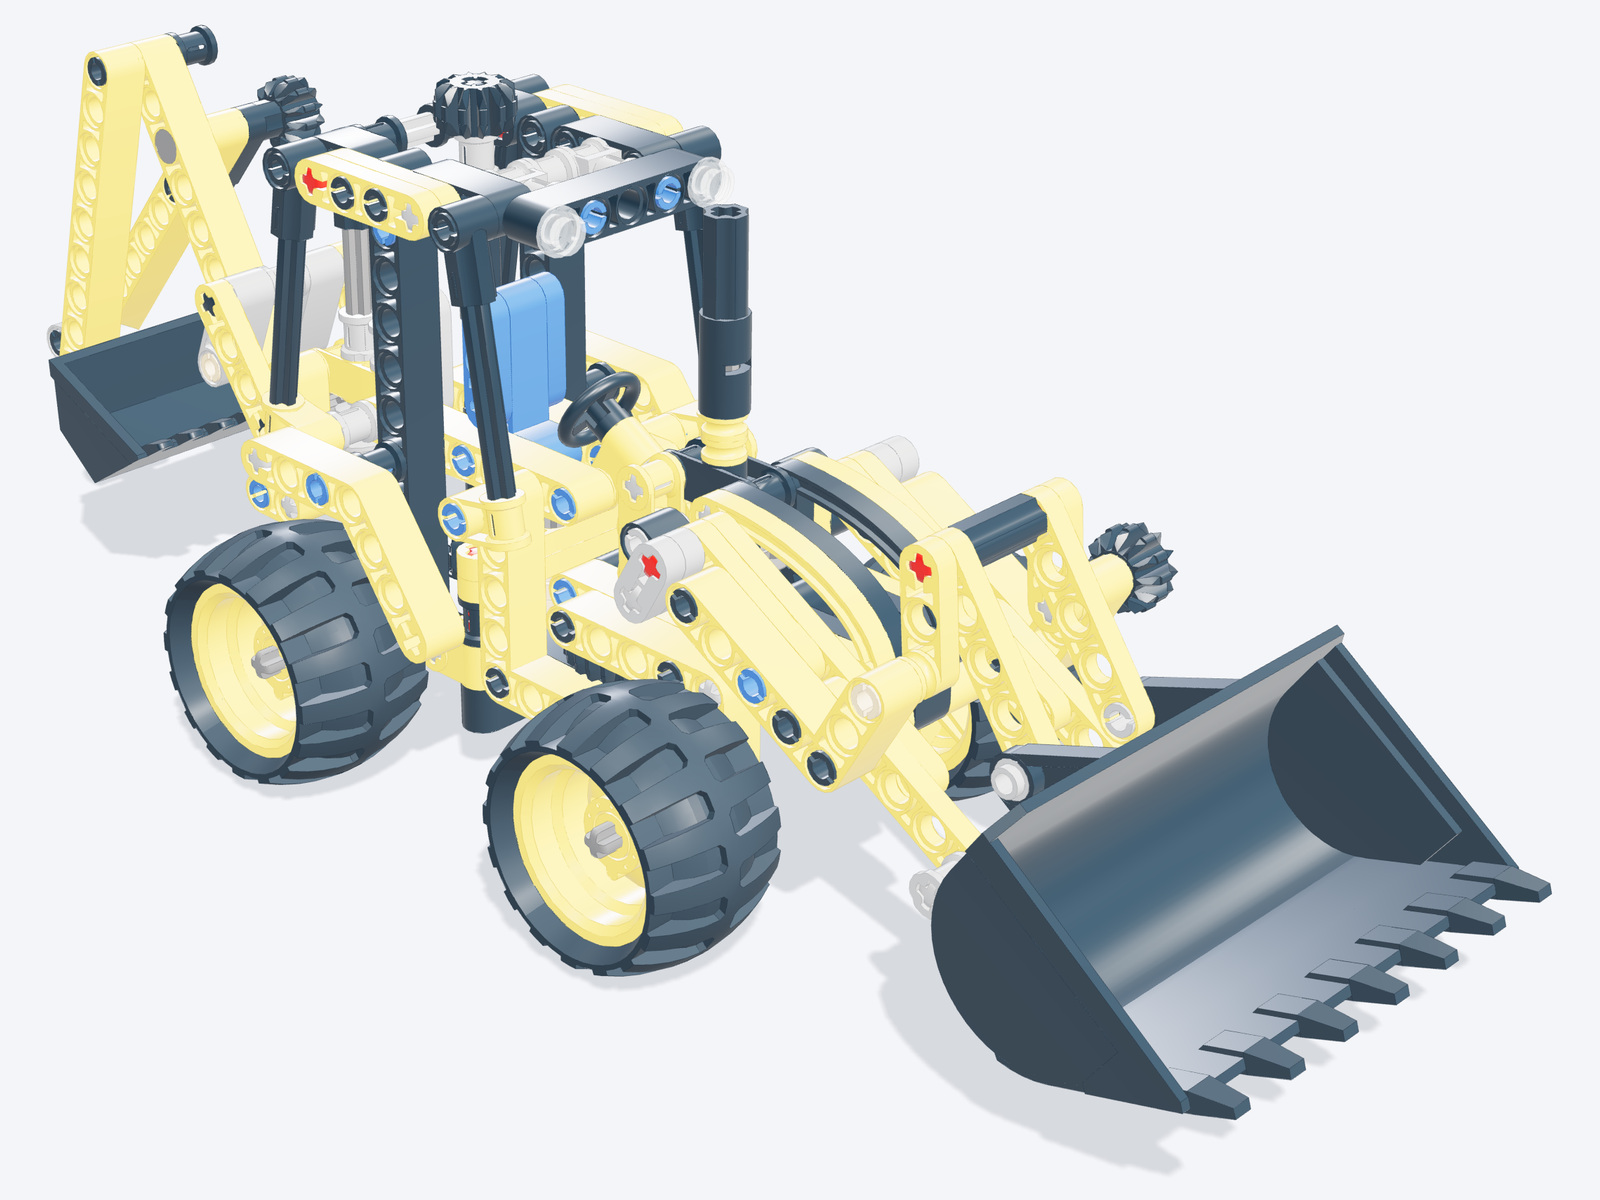
\includegraphics[width=.65\linewidth]{figures-v2/omr-42004-iso.jpg}\end{center}
\paragraph{Attribution.}Tomas Kralicek [RabbiT\_CZ]. CC BY 2.0.\par\url{https://library.ldraw.org/library/omr/42004-1.mpd}
\paragraph{Source SHA256.}\path{a32b924f302a1c028c1131f78e438ad2d78e70a041999690a1e4285e851f7dbf}
\paragraph{Connector records.}stud: 3; axle: 333; hinge: 1; fixed: 16; ball: 0
\paragraph{Public input lock.}\path{9554985a69f01e43f2836b31da3877455f1fa3d0f7f385b57b511812c06645d4}
\paragraph{Status.}Source preservation does not certify stability. Reference outputs below are internal review material. Full model inputs are the versioned public JSON and numbered PNGs.
\begin{enumerate}
\item \textbf{ld2-omr-42004-color-1}. Identify the original color of B0035; numbered isolation is allowed.
\par{\small color; visual; atomic; single-choice.\par\textit{Operands:} B0035 = brick\_000035\par\textit{Public evidence summary:} Numbered PNG: benchmark/ldraw-v2/inputs/views/ld2-omr-42004-color-1.png; structured input = \{\}.\par\textit{Options:} A: Blue; B: Tan; C: Rubber Black; D: Black\par\textit{Reference output:} \{"choiceId": "D"\}\par\textit{Derivation:} source colorName by rendered B-label; source oracle only\par\textit{Equivalence:} exact declared response\par\textit{Review:} pending required human review.}
\item \textbf{ld2-omr-42004-shape-match-1}. Ignoring color and pose, which numbered instance has the same LDraw part type as B0035?
\par{\small shape-match; visual; atomic; single-choice.\par\textit{Operands:} B0060 = brick\_000060, B0116 = brick\_000116, B0196 = brick\_000196, B0035 = brick\_000035, B0036 = brick\_000036\par\textit{Public evidence summary:} Numbered PNG: benchmark/ldraw-v2/inputs/views/ld2-omr-42004-shape-match-1.png; structured input = \{\}.\par\textit{Options:} A: B0196; B: B0116; C: B0036; D: B0060\par\textit{Reference output:} \{"choiceId": "C"\}\par\textit{Derivation:} source partNumber equality across labeled candidates; source oracle only\par\textit{Equivalence:} same source partNumber; ignore color and pose; perceptual equivalence pending\par\textit{Review:} pending required human review.}
\item \textbf{ld2-omr-42004-distance-1}. Using the supplied geometry bounding-box centers, which candidate is nearest to B0035?
\par{\small distance; source-data; atomic; single-choice.\par\textit{Operands:} B0233 = brick\_000233, B0035 = brick\_000035, B0116 = brick\_000116, B0171 = brick\_000171\par\textit{Public evidence summary:} \{"coordinateFrame": "Viewer world, millimeters, Euclidean distance", "centers": \{"B0035": [2, 32, 72], "B0171": [20, 57.456642, -92.888958], "B0233": [20.8, 22.3832, 119.5668], "B0116": [-18, 80, -4]\}\}\par\textit{Options:} A: B0171; B: B0116; C: B0233\par\textit{Reference output:} \{"choiceId": "C"\}\par\textit{Derivation:} Euclidean norm from public rounded centers\par\textit{Equivalence:} exact declared response\par\textit{Review:} machine checks passed; no human certification.}
\item \textbf{ld2-omr-42004-color-2}. Identify the original color of B0191; numbered isolation is allowed.
\par{\small color; visual; atomic; single-choice.\par\textit{Operands:} B0191 = brick\_000191\par\textit{Public evidence summary:} Numbered PNG: benchmark/ldraw-v2/inputs/views/ld2-omr-42004-color-2.png; structured input = \{\}.\par\textit{Options:} A: Light Bluish Grey; B: Black; C: Yellow; D: Rubber Black\par\textit{Reference output:} \{"choiceId": "B"\}\par\textit{Derivation:} source colorName by rendered B-label; source oracle only\par\textit{Equivalence:} exact declared response\par\textit{Review:} pending required human review.}
\item \textbf{ld2-omr-42004-shape-match-2}. Ignoring color and pose, which numbered instance has the same LDraw part type as B0191?
\par{\small shape-match; visual; atomic; single-choice.\par\textit{Operands:} B0141 = brick\_000141, B0039 = brick\_000039, B0235 = brick\_000235, B0191 = brick\_000191, B0047 = brick\_000047\par\textit{Public evidence summary:} Numbered PNG: benchmark/ldraw-v2/inputs/views/ld2-omr-42004-shape-match-2.png; structured input = \{\}.\par\textit{Options:} A: B0235; B: B0141; C: B0047; D: B0039\par\textit{Reference output:} \{"choiceId": "B"\}\par\textit{Derivation:} source partNumber equality across labeled candidates; source oracle only\par\textit{Equivalence:} same source partNumber; ignore color and pose; perceptual equivalence pending\par\textit{Review:} pending required human review.}
\item \textbf{ld2-omr-42004-distance-2}. Using the supplied geometry bounding-box centers, which candidate is nearest to B0191?
\par{\small distance; source-data; atomic; single-choice.\par\textit{Operands:} B0003 = brick\_000003, B0082 = brick\_000082, B0172 = brick\_000172, B0191 = brick\_000191\par\textit{Public evidence summary:} \{"coordinateFrame": "Viewer world, millimeters, Euclidean distance", "centers": \{"B0191": [-16, 52.39, -28.712], "B0003": [8, 0, 24], "B0172": [32, 63.4256, -88], "B0082": [24, 16, 24]\}\}\par\textit{Options:} A: B0003; B: B0172; C: B0082\par\textit{Reference output:} \{"choiceId": "C"\}\par\textit{Derivation:} Euclidean norm from public rounded centers\par\textit{Equivalence:} exact declared response\par\textit{Review:} machine checks passed; no human certification.}
\item \textbf{ld2-omr-42004-interface-1}. Classify the supplied connector record for B0047 and B0041. This does not certify load capacity.
\par{\small interface; connector-graph; metacognitive; single-choice.\par\textit{Operands:} B0041 = brick\_000041, B0047 = brick\_000047\par\textit{Public evidence summary:} \{"connectorRecord": \{"family": "axle", "aConnector": 0, "bConnector": 0\}, "scope": "Upstream connector tolerances and inset mesh intersections; unknown parts remain explicit, separate scene objects are not glued together; no load/force validation."\}\par\textit{Options:} A: axle; B: hinge; C: fixed; D: stud; E: ball\par\textit{Reference output:} \{"choiceId": "A"\}\par\textit{Derivation:} public connectorRecord.family equality\par\textit{Equivalence:} exact declared response\par\textit{Review:} machine checks passed; no human certification.}
\item \textbf{ld2-omr-42004-interface-2}. Classify the supplied connector record for B0239 and B0240. This does not certify load capacity.
\par{\small interface; connector-graph; metacognitive; single-choice.\par\textit{Operands:} B0240 = brick\_000240, B0239 = brick\_000239\par\textit{Public evidence summary:} \{"connectorRecord": \{"family": "fixed", "aConnector": 2, "bConnector": 1\}, "scope": "Upstream connector tolerances and inset mesh intersections; unknown parts remain explicit, separate scene objects are not glued together; no load/force validation."\}\par\textit{Options:} A: hinge; B: stud; C: axle; D: ball; E: fixed\par\textit{Reference output:} \{"choiceId": "E"\}\par\textit{Derivation:} public connectorRecord.family equality\par\textit{Equivalence:} exact declared response\par\textit{Review:} machine checks passed; no human certification.}
\item \textbf{ld2-omr-42004-interface-3}. Classify the supplied connector record for B0179 and B0178. This does not certify load capacity.
\par{\small interface; connector-graph; metacognitive; single-choice.\par\textit{Operands:} B0178 = brick\_000178, B0179 = brick\_000179\par\textit{Public evidence summary:} \{"connectorRecord": \{"family": "hinge", "aConnector": 1, "bConnector": 0\}, "scope": "Upstream connector tolerances and inset mesh intersections; unknown parts remain explicit, separate scene objects are not glued together; no load/force validation."\}\par\textit{Options:} A: stud; B: ball; C: hinge; D: fixed; E: axle\par\textit{Reference output:} \{"choiceId": "C"\}\par\textit{Derivation:} public connectorRecord.family equality\par\textit{Equivalence:} exact declared response\par\textit{Review:} machine checks passed; no human certification.}
\item \textbf{ld2-omr-42004-interface-4}. Classify the supplied connector record for B0146 and B0145. This does not certify load capacity.
\par{\small interface; connector-graph; metacognitive; single-choice.\par\textit{Operands:} B0146 = brick\_000146, B0145 = brick\_000145\par\textit{Public evidence summary:} \{"connectorRecord": \{"family": "stud", "aConnector": 1, "bConnector": 5\}, "scope": "Upstream connector tolerances and inset mesh intersections; unknown parts remain explicit, separate scene objects are not glued together; no load/force validation."\}\par\textit{Options:} A: fixed; B: stud; C: axle; D: hinge; E: ball\par\textit{Reference output:} \{"choiceId": "B"\}\par\textit{Derivation:} public connectorRecord.family equality\par\textit{Equivalence:} exact declared response\par\textit{Review:} machine checks passed; no human certification.}
\item \textbf{ld2-omr-42004-neighbors-1}. Select every candidate directly adjacent to B0192 in the supplied connector graph.
\par{\small neighbors; connector-graph; metacognitive; multiple-choice.\par\textit{Operands:} B0015 = brick\_000015, B0191 = brick\_000191, B0129 = brick\_000129, B0099 = brick\_000099, B0192 = brick\_000192\par\textit{Public evidence summary:} 2 unique undirected pairs\par\textit{Options:} A: B0129; B: B0015; C: B0191; D: B0099\par\textit{Reference output:} \{"choiceIds": ["A", "C"]\}\par\textit{Derivation:} public incident edge endpoint set\par\textit{Equivalence:} unordered exact set; duplicate IDs invalid\par\textit{Review:} machine checks passed; no human certification.}
\item \textbf{ld2-omr-42004-graph-removal-1}. Delete B0192 and its incident edges from this local graph. How many connected components remain? Do not infer physical extractability.
\par{\small graph-removal; connector-graph; graph-internal; integer.\par\textit{Operands:} B0099 = brick\_000099, B0129 = brick\_000129, B0192 = brick\_000192, B0015 = brick\_000015, B0191 = brick\_000191\par\textit{Public evidence summary:} 2 unique undirected pairs; 5 nodes\par\textit{Reference output:} \{"value": 4\}\par\textit{Derivation:} union-find component count after public target deletion\par\textit{Equivalence:} exact declared response\par\textit{Review:} machine checks passed; no human certification.}
\item \textbf{ld2-omr-42004-neighbors-2}. Select every candidate directly adjacent to B0180 in the supplied connector graph.
\par{\small neighbors; connector-graph; metacognitive; multiple-choice.\par\textit{Operands:} B0176 = brick\_000176, B0210 = brick\_000210, B0173 = brick\_000173, B0180 = brick\_000180, B0011 = brick\_000011\par\textit{Public evidence summary:} 2 unique undirected pairs\par\textit{Options:} A: B0176; B: B0011; C: B0173; D: B0210\par\textit{Reference output:} \{"choiceIds": ["A", "C"]\}\par\textit{Derivation:} public incident edge endpoint set\par\textit{Equivalence:} unordered exact set; duplicate IDs invalid\par\textit{Review:} machine checks passed; no human certification.}
\item \textbf{ld2-omr-42004-graph-removal-2}. Delete B0180 and its incident edges from this local graph. How many connected components remain? Do not infer physical extractability.
\par{\small graph-removal; connector-graph; graph-internal; integer.\par\textit{Operands:} B0011 = brick\_000011, B0210 = brick\_000210, B0173 = brick\_000173, B0176 = brick\_000176, B0180 = brick\_000180\par\textit{Public evidence summary:} 2 unique undirected pairs; 5 nodes\par\textit{Reference output:} \{"value": 4\}\par\textit{Derivation:} union-find component count after public target deletion\par\textit{Equivalence:} exact declared response\par\textit{Review:} machine checks passed; no human certification.}
\item \textbf{ld2-omr-42004-evidence-limit-1}. Only source geometry, connector matching and mesh intersection audits are available. Without mass, friction, material or dynamic tests, is gravitational stability established?
\par{\small evidence-limit; source-data; metacognitive; single-choice.\par\textit{Operands:} none\par\textit{Public evidence summary:} \{"available": ["Original CAD", "Connector inference", "Inset-mesh intersection candidates"]\}\par\textit{Options:} A: Established; B: Not established by this evidence\par\textit{Reference output:} \{"choiceId": "B"\}\par\textit{Derivation:} fixed epistemic control label\par\textit{Equivalence:} exact declared response\par\textit{Review:} machine checks passed; no human certification.}
\item \textbf{ld2-omr-42004-source-step-1}. At which expanded author step does B0007 first appear in the supplied source-step table? Source order is not a collision-free assembly proof.
\par{\small source-step; source-data; procedural; single-choice.\par\textit{Operands:} B0001 = brick\_000001, B0007 = brick\_000007\par\textit{Public evidence summary:} 2 supplied author-step records; exact table in public JSON\par\textit{Options:} A: 73; B: 4; C: 11; D: 81\par\textit{Reference output:} \{"choiceId": "B"\}\par\textit{Derivation:} minimum public step index containing target\par\textit{Equivalence:} exact declared response\par\textit{Review:} machine checks passed; no human certification.}
\item \textbf{ld2-omr-42004-source-step-2}. At which expanded author step does B0150 first appear in the supplied source-step table? Source order is not a collision-free assembly proof.
\par{\small source-step; source-data; procedural; single-choice.\par\textit{Operands:} B0150 = brick\_000150, B0001 = brick\_000001\par\textit{Public evidence summary:} 2 supplied author-step records; exact table in public JSON\par\textit{Options:} A: 80; B: 49; C: 20; D: 43\par\textit{Reference output:} \{"choiceId": "B"\}\par\textit{Derivation:} minimum public step index containing target\par\textit{Equivalence:} exact declared response\par\textit{Review:} pending required human review.}
\item \textbf{ld2-omr-42004-source-sequence-1}. Reveal the supplied source-step window in author order. Actions change visibility only, without simulating insertion trajectories.
\par{\small source-sequence; scene-edit; procedural; actions.\par\textit{Operands:} B0007 = brick\_000007, B0010 = brick\_000010, B0012 = brick\_000012, B0002 = brick\_000002, B0013 = brick\_000013, B0003 = brick\_000003, B0011 = brick\_000011, B0001 = brick\_000001, B0008 = brick\_000008, B0004 = brick\_000004, B0005 = brick\_000005, B0006 = brick\_000006, B0014 = brick\_000014, B0009 = brick\_000009, B0015 = brick\_000015\par\textit{Public evidence summary:} 6 public actions; budget 6; \{"initialFacts": ["start"], "goalFacts": ["done-6"], "absentFacts": []\}\par\textit{Reference output:} \{"actionIds": ["step-1", "step-2", "step-3", "step-4", "step-5", "step-6"]\}\par\textit{Derivation:} public precondition solver\par\textit{Equivalence:} any legal sequence reaching all goals within budget; display-only semantics\par\textit{Review:} pending required human review.}
\item \textbf{ld2-omr-42004-restore-instance-1}. The display copy hides B0035. Restore only that numbered instance, preserving all other instances and source poses.
\par{\small restore-instance; scene-edit; procedural; actions.\par\textit{Operands:} B0001 = brick\_000001, B0035 = brick\_000035\par\textit{Public evidence summary:} 2 public actions; budget 1; \{"initialFacts": ["missing-brick\_000035", "present-brick\_000001"], "goalFacts": ["present-brick\_000035", "present-brick\_000001"], "absentFacts": ["missing-brick\_000035"]\}\par\textit{Reference output:} \{"actionIds": ["restore-B0035"]\}\par\textit{Derivation:} public precondition solver\par\textit{Equivalence:} any legal sequence reaching all goals within budget; display-only semantics\par\textit{Review:} machine checks passed; no human certification.}
\item \textbf{ld2-omr-42004-restore-instance-2}. The display copy hides B0191. Restore only that numbered instance, preserving all other instances and source poses.
\par{\small restore-instance; scene-edit; procedural; actions.\par\textit{Operands:} B0001 = brick\_000001, B0191 = brick\_000191\par\textit{Public evidence summary:} 2 public actions; budget 1; \{"initialFacts": ["missing-brick\_000191", "present-brick\_000001"], "goalFacts": ["present-brick\_000191", "present-brick\_000001"], "absentFacts": ["missing-brick\_000191"]\}\par\textit{Reference output:} \{"actionIds": ["restore-B0191"]\}\par\textit{Derivation:} public precondition solver\par\textit{Equivalence:} any legal sequence reaching all goals within budget; display-only semantics\par\textit{Review:} machine checks passed; no human certification.}
\end{enumerate}
\clearpage\section{42061: Telehandler}
261 source instances; 20 tasks; D2 size band. 72 type strings; 14 color codes; 13 unsupported instances; 3 intersection candidates. 44 expanded author steps. Independent reparse: passed.
\begin{center}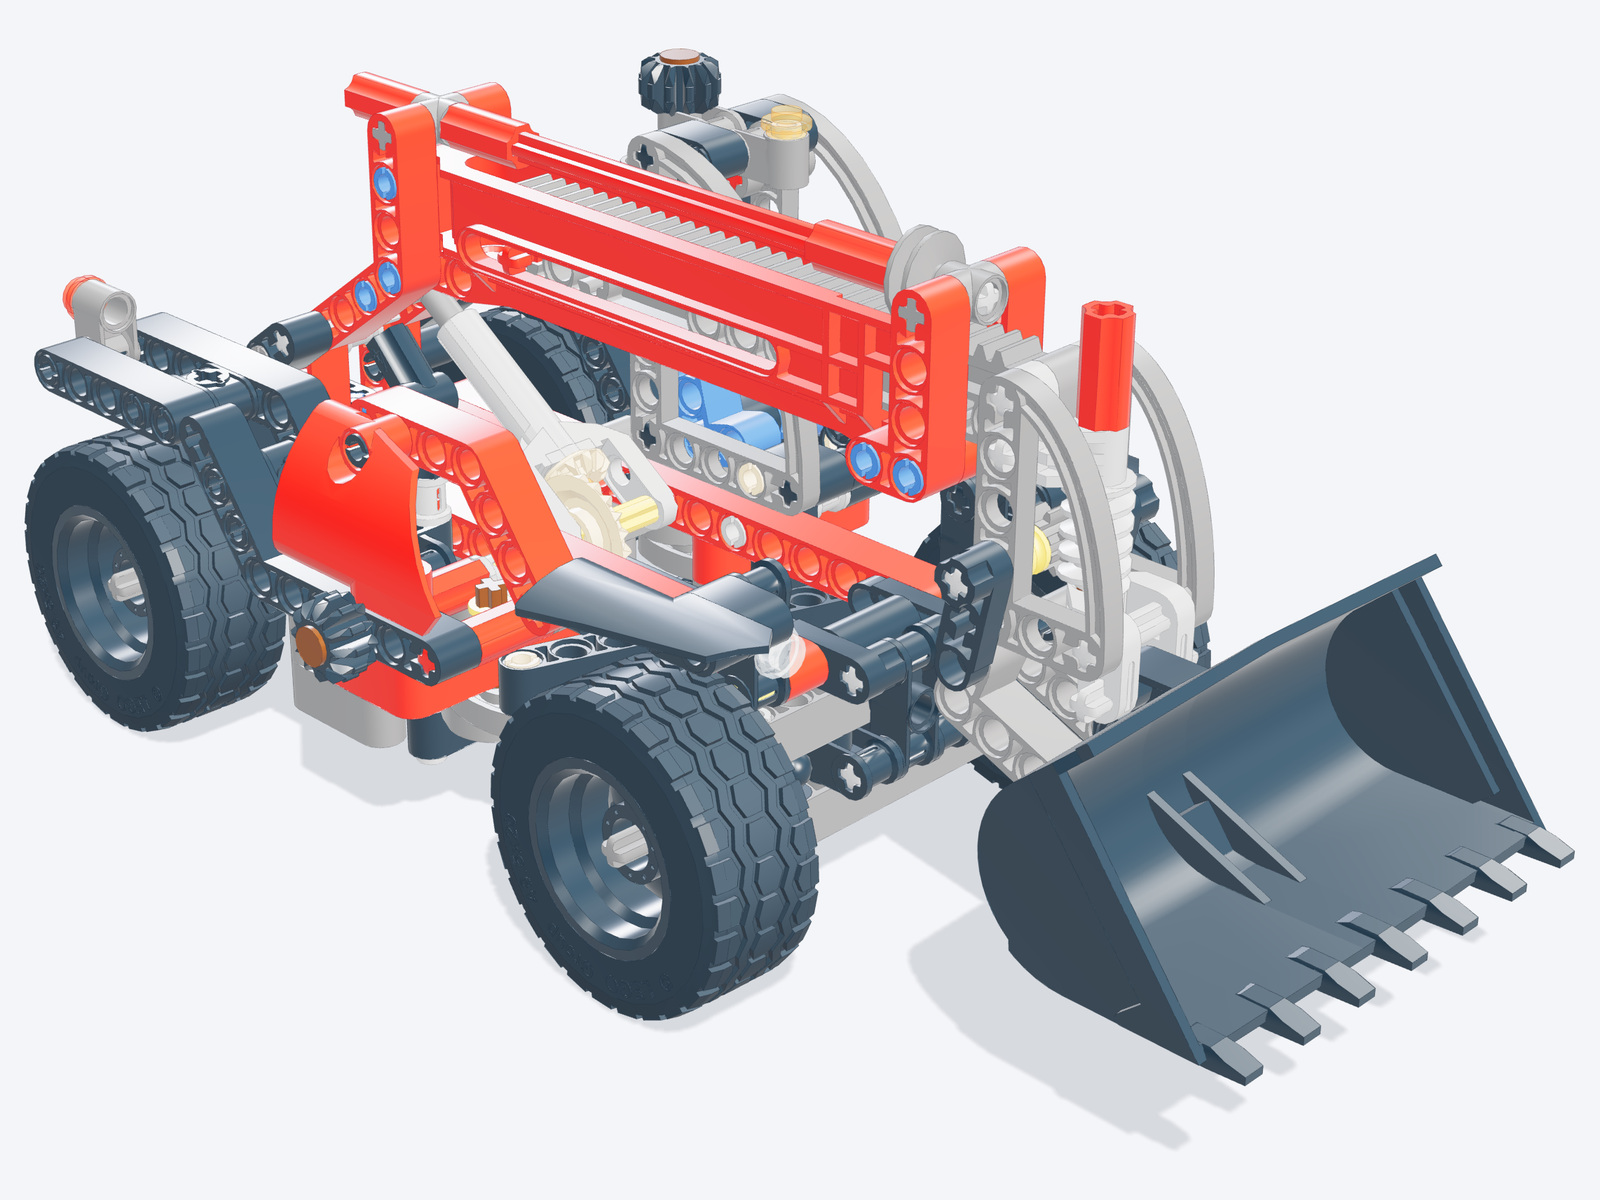
\includegraphics[width=.65\linewidth]{figures-v2/omr-42061-iso.jpg}\end{center}
\paragraph{Attribution.}Philippe Hurbain [Philo]. CC BY 2.0.\par\url{https://library.ldraw.org/library/omr/42061-1.mpd}
\paragraph{Source SHA256.}\path{040a7bd002747abebebca005d7d049c902ffd39d2b102c180458fcfdd94f369c}
\paragraph{Connector records.}stud: 5; axle: 317; hinge: 0; fixed: 16; ball: 0
\paragraph{Public input lock.}\path{e8bc90794cfa1e761053e31187ccc668dc86fd25fb6b674f9a29736f607c6dca}
\paragraph{Status.}Source preservation does not certify stability. Reference outputs below are internal review material. Full model inputs are the versioned public JSON and numbered PNGs.
\begin{enumerate}
\item \textbf{ld2-omr-42061-color-1}. Identify the original color of B0088; numbered isolation is allowed.
\par{\small color; visual; atomic; single-choice.\par\textit{Operands:} B0088 = brick\_000088\par\textit{Public evidence summary:} Numbered PNG: benchmark/ldraw-v2/inputs/views/ld2-omr-42061-color-1.png; structured input = \{\}.\par\textit{Options:} A: Blue; B: Tan; C: Rubber Black; D: Dark Bluish Grey\par\textit{Reference output:} \{"choiceId": "A"\}\par\textit{Derivation:} source colorName by rendered B-label; source oracle only\par\textit{Equivalence:} exact declared response\par\textit{Review:} pending required human review.}
\item \textbf{ld2-omr-42061-shape-match-1}. Ignoring color and pose, which numbered instance has the same LDraw part type as B0088?
\par{\small shape-match; visual; atomic; single-choice.\par\textit{Operands:} B0089 = brick\_000089, B0088 = brick\_000088, B0235 = brick\_000235, B0064 = brick\_000064, B0166 = brick\_000166\par\textit{Public evidence summary:} Numbered PNG: benchmark/ldraw-v2/inputs/views/ld2-omr-42061-shape-match-1.png; structured input = \{\}.\par\textit{Options:} A: B0235; B: B0064; C: B0166; D: B0089\par\textit{Reference output:} \{"choiceId": "D"\}\par\textit{Derivation:} source partNumber equality across labeled candidates; source oracle only\par\textit{Equivalence:} same source partNumber; ignore color and pose; perceptual equivalence pending\par\textit{Review:} pending required human review.}
\item \textbf{ld2-omr-42061-distance-1}. Using the supplied geometry bounding-box centers, which candidate is nearest to B0088?
\par{\small distance; source-data; atomic; single-choice.\par\textit{Operands:} B0088 = brick\_000088, B0203 = brick\_000203, B0194 = brick\_000194, B0021 = brick\_000021\par\textit{Public evidence summary:} \{"coordinateFrame": "Viewer world, millimeters, Euclidean distance", "centers": \{"B0088": [8, 92, 25.6], "B0021": [-8, 24.8, 76], "B0194": [8, 100, 129.6], "B0203": [39.9992, 48.8016, 56]\}\}\par\textit{Options:} A: B0021; B: B0194; C: B0203\par\textit{Reference output:} \{"choiceId": "C"\}\par\textit{Derivation:} Euclidean norm from public rounded centers\par\textit{Equivalence:} exact declared response\par\textit{Review:} machine checks passed; no human certification.}
\item \textbf{ld2-omr-42061-color-2}. Identify the original color of B0104; numbered isolation is allowed.
\par{\small color; visual; atomic; single-choice.\par\textit{Operands:} B0104 = brick\_000104\par\textit{Public evidence summary:} Numbered PNG: benchmark/ldraw-v2/inputs/views/ld2-omr-42061-color-2.png; structured input = \{\}.\par\textit{Options:} A: Light Bluish Grey; B: Black; C: Red; D: Reddish Brown\par\textit{Reference output:} \{"choiceId": "A"\}\par\textit{Derivation:} source colorName by rendered B-label; source oracle only\par\textit{Equivalence:} exact declared response\par\textit{Review:} pending required human review.}
\item \textbf{ld2-omr-42061-shape-match-2}. Ignoring color and pose, which numbered instance has the same LDraw part type as B0104?
\par{\small shape-match; visual; atomic; single-choice.\par\textit{Operands:} B0174 = brick\_000174, B0183 = brick\_000183, B0151 = brick\_000151, B0063 = brick\_000063, B0104 = brick\_000104\par\textit{Public evidence summary:} Numbered PNG: benchmark/ldraw-v2/inputs/views/ld2-omr-42061-shape-match-2.png; structured input = \{\}.\par\textit{Options:} A: B0063; B: B0183; C: B0151; D: B0174\par\textit{Reference output:} \{"choiceId": "B"\}\par\textit{Derivation:} source partNumber equality across labeled candidates; source oracle only\par\textit{Equivalence:} same source partNumber; ignore color and pose; perceptual equivalence pending\par\textit{Review:} pending required human review.}
\item \textbf{ld2-omr-42061-distance-2}. Using the supplied geometry bounding-box centers, which candidate is nearest to B0104?
\par{\small distance; source-data; atomic; single-choice.\par\textit{Operands:} B0252 = brick\_000252, B0104 = brick\_000104, B0204 = brick\_000204, B0134 = brick\_000134\par\textit{Public evidence summary:} \{"coordinateFrame": "Viewer world, millimeters, Euclidean distance", "centers": \{"B0104": [8, 61.6, 6.4], "B0252": [40.0004, 88.9044, 48], "B0204": [39.9992, 48.8016, 88], "B0134": [-40, 50.381801, 52.818109]\}\}\par\textit{Options:} A: B0252; B: B0204; C: B0134\par\textit{Reference output:} \{"choiceId": "A"\}\par\textit{Derivation:} Euclidean norm from public rounded centers\par\textit{Equivalence:} exact declared response\par\textit{Review:} machine checks passed; no human certification.}
\item \textbf{ld2-omr-42061-interface-1}. Classify the supplied connector record for B0237 and B0236. This does not certify load capacity.
\par{\small interface; connector-graph; metacognitive; single-choice.\par\textit{Operands:} B0237 = brick\_000237, B0236 = brick\_000236\par\textit{Public evidence summary:} \{"connectorRecord": \{"family": "axle", "aConnector": 1, "bConnector": 0\}, "scope": "Upstream connector tolerances and inset mesh intersections; unknown parts remain explicit, separate scene objects are not glued together; no load/force validation."\}\par\textit{Options:} A: stud; B: axle; C: fixed; D: ball; E: hinge\par\textit{Reference output:} \{"choiceId": "B"\}\par\textit{Derivation:} public connectorRecord.family equality\par\textit{Equivalence:} exact declared response\par\textit{Review:} machine checks passed; no human certification.}
\item \textbf{ld2-omr-42061-interface-2}. Classify the supplied connector record for B0260 and B0261. This does not certify load capacity.
\par{\small interface; connector-graph; metacognitive; single-choice.\par\textit{Operands:} B0261 = brick\_000261, B0260 = brick\_000260\par\textit{Public evidence summary:} \{"connectorRecord": \{"family": "fixed", "aConnector": 2, "bConnector": 0\}, "scope": "Upstream connector tolerances and inset mesh intersections; unknown parts remain explicit, separate scene objects are not glued together; no load/force validation."\}\par\textit{Options:} A: hinge; B: ball; C: fixed; D: axle; E: stud\par\textit{Reference output:} \{"choiceId": "C"\}\par\textit{Derivation:} public connectorRecord.family equality\par\textit{Equivalence:} exact declared response\par\textit{Review:} machine checks passed; no human certification.}
\item \textbf{ld2-omr-42061-interface-3}. Classify the supplied connector record for B0210 and B0211. This does not certify load capacity.
\par{\small interface; connector-graph; metacognitive; single-choice.\par\textit{Operands:} B0211 = brick\_000211, B0210 = brick\_000210\par\textit{Public evidence summary:} \{"connectorRecord": \{"family": "stud", "aConnector": 2, "bConnector": 0\}, "scope": "Upstream connector tolerances and inset mesh intersections; unknown parts remain explicit, separate scene objects are not glued together; no load/force validation."\}\par\textit{Options:} A: stud; B: axle; C: fixed; D: ball; E: hinge\par\textit{Reference output:} \{"choiceId": "A"\}\par\textit{Derivation:} public connectorRecord.family equality\par\textit{Equivalence:} exact declared response\par\textit{Review:} machine checks passed; no human certification.}
\item \textbf{ld2-omr-42061-neighbors-1}. Select every candidate directly adjacent to B0130 in the supplied connector graph.
\par{\small neighbors; connector-graph; metacognitive; multiple-choice.\par\textit{Operands:} B0172 = brick\_000172, B0128 = brick\_000128, B0132 = brick\_000132, B0130 = brick\_000130, B0117 = brick\_000117\par\textit{Public evidence summary:} 2 unique undirected pairs\par\textit{Options:} A: B0128; B: B0117; C: B0132; D: B0172\par\textit{Reference output:} \{"choiceIds": ["A", "C"]\}\par\textit{Derivation:} public incident edge endpoint set\par\textit{Equivalence:} unordered exact set; duplicate IDs invalid\par\textit{Review:} machine checks passed; no human certification.}
\item \textbf{ld2-omr-42061-graph-removal-1}. Delete B0130 and its incident edges from this local graph. How many connected components remain? Do not infer physical extractability.
\par{\small graph-removal; connector-graph; graph-internal; integer.\par\textit{Operands:} B0117 = brick\_000117, B0172 = brick\_000172, B0128 = brick\_000128, B0132 = brick\_000132, B0130 = brick\_000130\par\textit{Public evidence summary:} 2 unique undirected pairs; 5 nodes\par\textit{Reference output:} \{"value": 4\}\par\textit{Derivation:} union-find component count after public target deletion\par\textit{Equivalence:} exact declared response\par\textit{Review:} machine checks passed; no human certification.}
\item \textbf{ld2-omr-42061-neighbors-2}. Select every candidate directly adjacent to B0075 in the supplied connector graph.
\par{\small neighbors; connector-graph; metacognitive; multiple-choice.\par\textit{Operands:} B0026 = brick\_000026, B0079 = brick\_000079, B0076 = brick\_000076, B0067 = brick\_000067, B0075 = brick\_000075\par\textit{Public evidence summary:} 2 unique undirected pairs\par\textit{Options:} A: B0067; B: B0026; C: B0076; D: B0079\par\textit{Reference output:} \{"choiceIds": ["C", "D"]\}\par\textit{Derivation:} public incident edge endpoint set\par\textit{Equivalence:} unordered exact set; duplicate IDs invalid\par\textit{Review:} machine checks passed; no human certification.}
\item \textbf{ld2-omr-42061-graph-removal-2}. Delete B0075 and its incident edges from this local graph. How many connected components remain? Do not infer physical extractability.
\par{\small graph-removal; connector-graph; graph-internal; integer.\par\textit{Operands:} B0067 = brick\_000067, B0026 = brick\_000026, B0076 = brick\_000076, B0079 = brick\_000079, B0075 = brick\_000075\par\textit{Public evidence summary:} 2 unique undirected pairs; 5 nodes\par\textit{Reference output:} \{"value": 4\}\par\textit{Derivation:} union-find component count after public target deletion\par\textit{Equivalence:} exact declared response\par\textit{Review:} machine checks passed; no human certification.}
\item \textbf{ld2-omr-42061-coverage-1}. Which numbered instance lacks a connector definition in the coverage record, so this audit cannot establish that it is floating?
\par{\small coverage; source-data; metacognitive; single-choice.\par\textit{Operands:} B0088 = brick\_000088, B0066 = brick\_000066, B0104 = brick\_000104, B0212 = brick\_000212\par\textit{Public evidence summary:} \{"coverage": [\{"label": "B0088", "supported": true\}, \{"label": "B0066", "supported": false\}, \{"label": "B0104", "supported": true\}, \{"label": "B0212", "supported": true\}]\}\par\textit{Options:} A: B0088; B: B0212; C: B0066; D: B0104\par\textit{Reference output:} \{"choiceId": "C"\}\par\textit{Derivation:} public supported=false record\par\textit{Equivalence:} exact declared response\par\textit{Review:} pending required human review.}
\item \textbf{ld2-omr-42061-evidence-limit-1}. Only source geometry, connector matching and mesh intersection audits are available. Without mass, friction, material or dynamic tests, is gravitational stability established?
\par{\small evidence-limit; source-data; metacognitive; single-choice.\par\textit{Operands:} none\par\textit{Public evidence summary:} \{"available": ["Original CAD", "Connector inference", "Inset-mesh intersection candidates"]\}\par\textit{Options:} A: Established; B: Not established by this evidence\par\textit{Reference output:} \{"choiceId": "B"\}\par\textit{Derivation:} fixed epistemic control label\par\textit{Equivalence:} exact declared response\par\textit{Review:} machine checks passed; no human certification.}
\item \textbf{ld2-omr-42061-source-step-1}. At which expanded author step does B0041 first appear in the supplied source-step table? Source order is not a collision-free assembly proof.
\par{\small source-step; source-data; procedural; single-choice.\par\textit{Operands:} B0001 = brick\_000001, B0041 = brick\_000041\par\textit{Public evidence summary:} 2 supplied author-step records; exact table in public JSON\par\textit{Options:} A: 8; B: 7; C: 32; D: 5\par\textit{Reference output:} \{"choiceId": "A"\}\par\textit{Derivation:} minimum public step index containing target\par\textit{Equivalence:} exact declared response\par\textit{Review:} machine checks passed; no human certification.}
\item \textbf{ld2-omr-42061-source-step-2}. At which expanded author step does B0245 first appear in the supplied source-step table? Source order is not a collision-free assembly proof.
\par{\small source-step; source-data; procedural; single-choice.\par\textit{Operands:} B0001 = brick\_000001, B0245 = brick\_000245\par\textit{Public evidence summary:} 2 supplied author-step records; exact table in public JSON\par\textit{Options:} A: 29; B: 43; C: 42; D: 2\par\textit{Reference output:} \{"choiceId": "C"\}\par\textit{Derivation:} minimum public step index containing target\par\textit{Equivalence:} exact declared response\par\textit{Review:} machine checks passed; no human certification.}
\item \textbf{ld2-omr-42061-source-sequence-1}. Reveal the supplied source-step window in author order. Actions change visibility only, without simulating insertion trajectories.
\par{\small source-sequence; scene-edit; procedural; actions.\par\textit{Operands:} B0022 = brick\_000022, B0002 = brick\_000002, B0031 = brick\_000031, B0035 = brick\_000035, B0028 = brick\_000028, B0006 = brick\_000006, B0024 = brick\_000024, B0001 = brick\_000001, B0034 = brick\_000034, B0023 = brick\_000023, B0007 = brick\_000007, B0005 = brick\_000005, B0003 = brick\_000003, B0010 = brick\_000010, B0025 = brick\_000025, B0032 = brick\_000032, B0011 = brick\_000011, B0013 = brick\_000013, B0012 = brick\_000012, B0009 = brick\_000009, B0020 = brick\_000020, B0030 = brick\_000030, B0019 = brick\_000019, B0033 = brick\_000033, B0029 = brick\_000029, B0021 = brick\_000021, B0017 = brick\_000017, B0027 = brick\_000027, B0026 = brick\_000026, B0008 = brick\_000008, B0016 = brick\_000016, B0018 = brick\_000018, B0015 = brick\_000015, B0004 = brick\_000004, B0014 = brick\_000014\par\textit{Public evidence summary:} 6 public actions; budget 6; \{"initialFacts": ["start"], "goalFacts": ["done-6"], "absentFacts": []\}\par\textit{Reference output:} \{"actionIds": ["step-1", "step-2", "step-3", "step-4", "step-5", "step-6"]\}\par\textit{Derivation:} public precondition solver\par\textit{Equivalence:} any legal sequence reaching all goals within budget; display-only semantics\par\textit{Review:} machine checks passed; no human certification.}
\item \textbf{ld2-omr-42061-restore-instance-1}. The display copy hides B0088. Restore only that numbered instance, preserving all other instances and source poses.
\par{\small restore-instance; scene-edit; procedural; actions.\par\textit{Operands:} B0001 = brick\_000001, B0088 = brick\_000088\par\textit{Public evidence summary:} 2 public actions; budget 1; \{"initialFacts": ["missing-brick\_000088", "present-brick\_000001"], "goalFacts": ["present-brick\_000088", "present-brick\_000001"], "absentFacts": ["missing-brick\_000088"]\}\par\textit{Reference output:} \{"actionIds": ["restore-B0088"]\}\par\textit{Derivation:} public precondition solver\par\textit{Equivalence:} any legal sequence reaching all goals within budget; display-only semantics\par\textit{Review:} machine checks passed; no human certification.}
\item \textbf{ld2-omr-42061-restore-instance-2}. The display copy hides B0104. Restore only that numbered instance, preserving all other instances and source poses.
\par{\small restore-instance; scene-edit; procedural; actions.\par\textit{Operands:} B0001 = brick\_000001, B0104 = brick\_000104\par\textit{Public evidence summary:} 2 public actions; budget 1; \{"initialFacts": ["missing-brick\_000104", "present-brick\_000001"], "goalFacts": ["present-brick\_000104", "present-brick\_000001"], "absentFacts": ["missing-brick\_000104"]\}\par\textit{Reference output:} \{"actionIds": ["restore-B0104"]\}\par\textit{Derivation:} public precondition solver\par\textit{Equivalence:} any legal sequence reaching all goals within budget; display-only semantics\par\textit{Review:} machine checks passed; no human certification.}
\end{enumerate}
\clearpage\section{31009: Small Cottage}
270 source instances; 20 tasks; D2 size band. 65 type strings; 18 color codes; 8 unsupported instances; 0 intersection candidates. 79 expanded author steps. Independent reparse: passed.
\begin{center}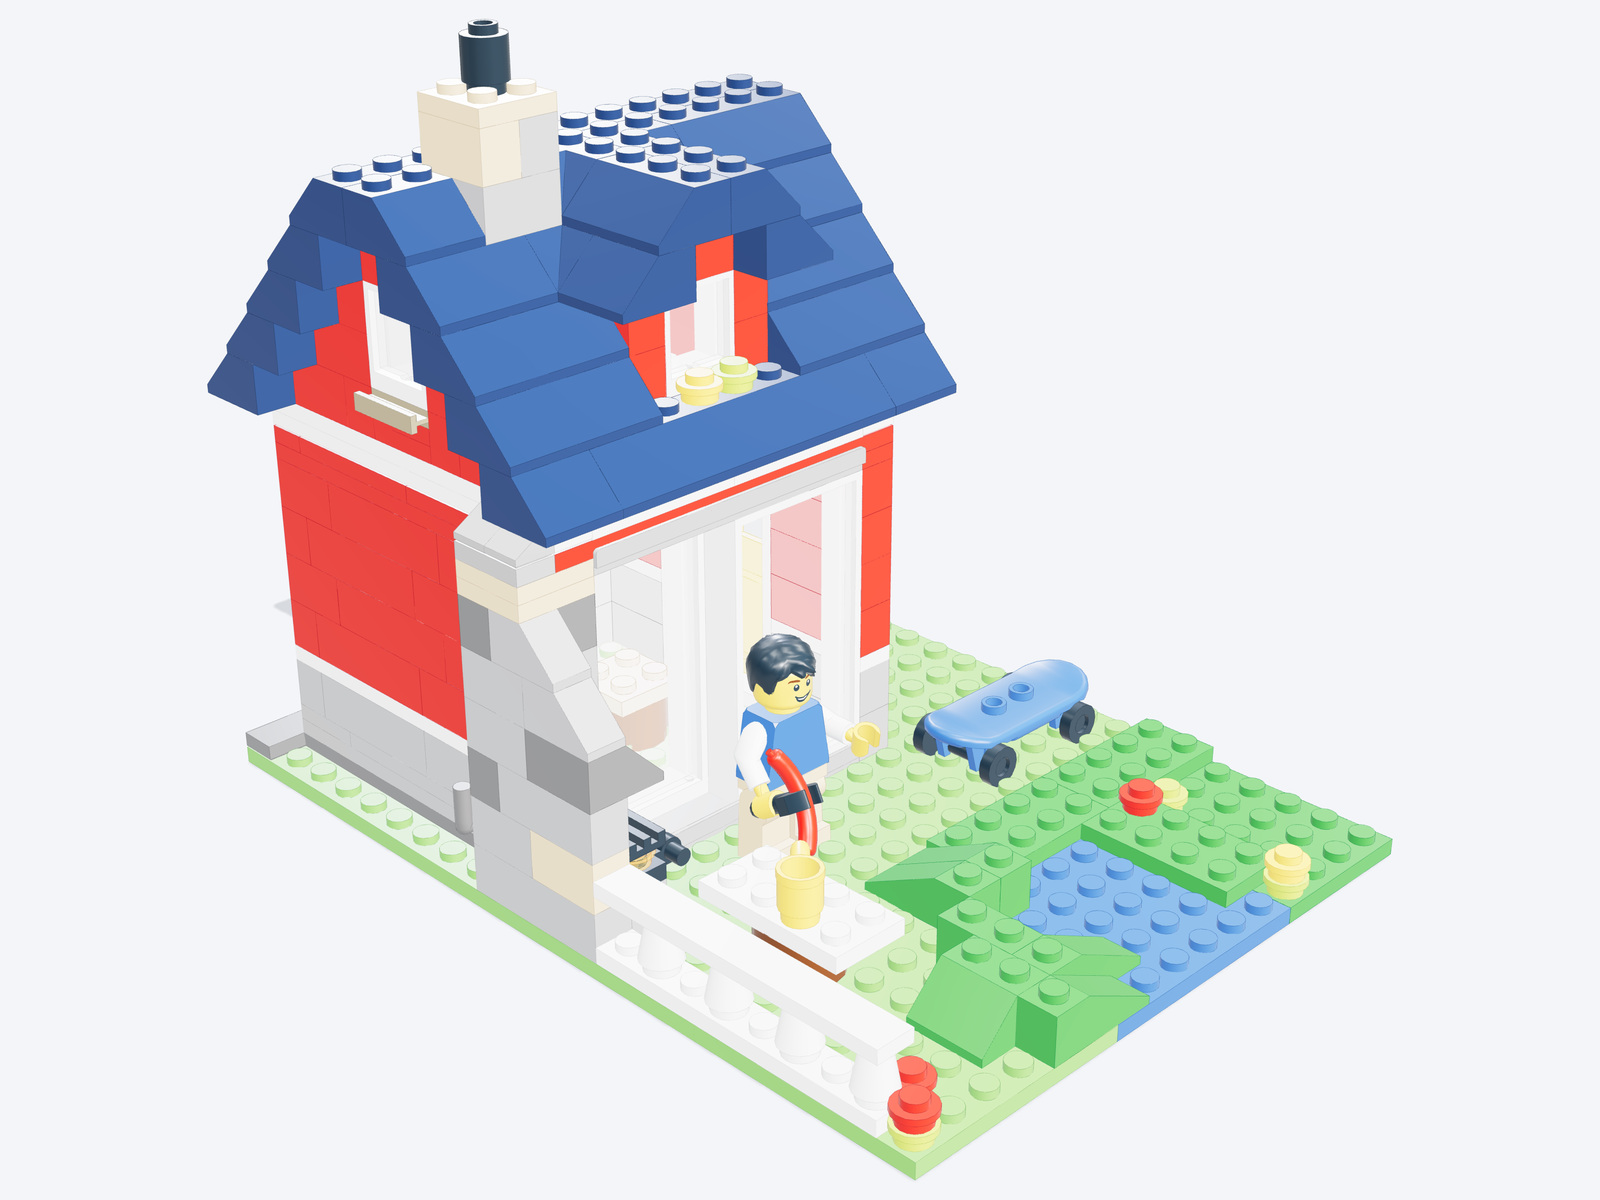
\includegraphics[width=.65\linewidth]{figures-v2/31009-iso.jpg}\end{center}
\paragraph{Attribution.}Stefan Frenz [smf]. CC BY 2.0.\par\url{https://library.ldraw.org/omr/sets/1164}
\paragraph{Source SHA256.}\path{97b83517b0e843f8071ea3e4e80fbe0c7897685a7f476d3ba83161bb1185333d}
\paragraph{Connector records.}stud: 772; axle: 3; hinge: 8; fixed: 2; ball: 0
\paragraph{Public input lock.}\path{668f9531ce10e4f9cab3684f6b2297998cb509e814750d6f57aaf9bb0a21844e}
\paragraph{Status.}Source preservation does not certify stability. Reference outputs below are internal review material. Full model inputs are the versioned public JSON and numbered PNGs.
\begin{enumerate}
\item \textbf{ld2-31009-color-1}. Identify the original color of B0163; numbered isolation is allowed.
\par{\small color; visual; atomic; single-choice.\par\textit{Operands:} B0163 = brick\_000163\par\textit{Public evidence summary:} Numbered PNG: benchmark/ldraw-v2/inputs/views/ld2-31009-color-1.png; structured input = \{\}.\par\textit{Options:} A: Trans Clear; B: Red; C: Medium Blue; D: Light Bluish Grey\par\textit{Reference output:} \{"choiceId": "B"\}\par\textit{Derivation:} source colorName by rendered B-label; source oracle only\par\textit{Equivalence:} exact declared response\par\textit{Review:} pending required human review.}
\item \textbf{ld2-31009-shape-match-1}. Ignoring color and pose, which numbered instance has the same LDraw part type as B0163?
\par{\small shape-match; visual; atomic; single-choice.\par\textit{Operands:} B0088 = brick\_000088, B0163 = brick\_000163, B0022 = brick\_000022, B0118 = brick\_000118, B0020 = brick\_000020\par\textit{Public evidence summary:} Numbered PNG: benchmark/ldraw-v2/inputs/views/ld2-31009-shape-match-1.png; structured input = \{\}.\par\textit{Options:} A: B0088; B: B0118; C: B0022; D: B0020\par\textit{Reference output:} \{"choiceId": "C"\}\par\textit{Derivation:} source partNumber equality across labeled candidates; source oracle only\par\textit{Equivalence:} same source partNumber; ignore color and pose; perceptual equivalence pending\par\textit{Review:} pending required human review.}
\item \textbf{ld2-31009-distance-1}. Using the supplied geometry bounding-box centers, which candidate is nearest to B0163?
\par{\small distance; source-data; atomic; single-choice.\par\textit{Operands:} B0163 = brick\_000163, B0145 = brick\_000145, B0063 = brick\_000063, B0200 = brick\_000200\par\textit{Public evidence summary:} \{"coordinateFrame": "Viewer world, millimeters, Euclidean distance", "centers": \{"B0163": [4, 79.2, -16], "B0200": [-32, 96.8, 12], "B0063": [-68, 40.8, 0], "B0145": [12, 15.2, -52]\}\}\par\textit{Options:} A: B0063; B: B0200; C: B0145\par\textit{Reference output:} \{"choiceId": "B"\}\par\textit{Derivation:} Euclidean norm from public rounded centers\par\textit{Equivalence:} exact declared response\par\textit{Review:} machine checks passed; no human certification.}
\item \textbf{ld2-31009-color-2}. Identify the original color of B0262; numbered isolation is allowed.
\par{\small color; visual; atomic; single-choice.\par\textit{Operands:} B0262 = brick\_000262\par\textit{Public evidence summary:} Numbered PNG: benchmark/ldraw-v2/inputs/views/ld2-31009-color-2.png; structured input = \{\}.\par\textit{Options:} A: Trans Clear; B: Blue; C: Dark Blue; D: Light Bluish Grey\par\textit{Reference output:} \{"choiceId": "B"\}\par\textit{Derivation:} source colorName by rendered B-label; source oracle only\par\textit{Equivalence:} exact declared response\par\textit{Review:} pending required human review.}
\item \textbf{ld2-31009-distance-2}. Using the supplied geometry bounding-box centers, which candidate is nearest to B0262?
\par{\small distance; source-data; atomic; single-choice.\par\textit{Operands:} B0262 = brick\_000262, B0235 = brick\_000235, B0085 = brick\_000085, B0099 = brick\_000099\par\textit{Public evidence summary:} \{"coordinateFrame": "Viewer world, millimeters, Euclidean distance", "centers": \{"B0262": [-32, 28, 35.6], "B0099": [12, 67.12, -28], "B0085": [-72, 56.8, 16], "B0235": [-76, 12, 100]\}\}\par\textit{Options:} A: B0085; B: B0099; C: B0235\par\textit{Reference output:} \{"choiceId": "A"\}\par\textit{Derivation:} Euclidean norm from public rounded centers\par\textit{Equivalence:} exact declared response\par\textit{Review:} machine checks passed; no human certification.}
\item \textbf{ld2-31009-interface-1}. Classify the supplied connector record for B0263 and B0262. This does not certify load capacity.
\par{\small interface; connector-graph; metacognitive; single-choice.\par\textit{Operands:} B0262 = brick\_000262, B0263 = brick\_000263\par\textit{Public evidence summary:} \{"connectorRecord": \{"family": "axle", "aConnector": 1, "bConnector": 0\}, "scope": "Upstream connector tolerances and inset mesh intersections; unknown parts remain explicit, separate scene objects are not glued together; no load/force validation."\}\par\textit{Options:} A: axle; B: hinge; C: stud; D: fixed; E: ball\par\textit{Reference output:} \{"choiceId": "A"\}\par\textit{Derivation:} public connectorRecord.family equality\par\textit{Equivalence:} exact declared response\par\textit{Review:} machine checks passed; no human certification.}
\item \textbf{ld2-31009-interface-2}. Classify the supplied connector record for B0261 and B0262. This does not certify load capacity.
\par{\small interface; connector-graph; metacognitive; single-choice.\par\textit{Operands:} B0261 = brick\_000261, B0262 = brick\_000262\par\textit{Public evidence summary:} \{"connectorRecord": \{"family": "fixed", "aConnector": 1, "bConnector": 1\}, "scope": "Upstream connector tolerances and inset mesh intersections; unknown parts remain explicit, separate scene objects are not glued together; no load/force validation."\}\par\textit{Options:} A: stud; B: axle; C: ball; D: fixed; E: hinge\par\textit{Reference output:} \{"choiceId": "D"\}\par\textit{Derivation:} public connectorRecord.family equality\par\textit{Equivalence:} exact declared response\par\textit{Review:} machine checks passed; no human certification.}
\item \textbf{ld2-31009-interface-3}. Classify the supplied connector record for B0259 and B0258. This does not certify load capacity.
\par{\small interface; connector-graph; metacognitive; single-choice.\par\textit{Operands:} B0259 = brick\_000259, B0258 = brick\_000258\par\textit{Public evidence summary:} \{"connectorRecord": \{"family": "hinge", "aConnector": 1, "bConnector": 2\}, "scope": "Upstream connector tolerances and inset mesh intersections; unknown parts remain explicit, separate scene objects are not glued together; no load/force validation."\}\par\textit{Options:} A: ball; B: fixed; C: axle; D: hinge; E: stud\par\textit{Reference output:} \{"choiceId": "D"\}\par\textit{Derivation:} public connectorRecord.family equality\par\textit{Equivalence:} exact declared response\par\textit{Review:} machine checks passed; no human certification.}
\item \textbf{ld2-31009-interface-4}. Classify the supplied connector record for B0064 and B0074. This does not certify load capacity.
\par{\small interface; connector-graph; metacognitive; single-choice.\par\textit{Operands:} B0074 = brick\_000074, B0064 = brick\_000064\par\textit{Public evidence summary:} \{"connectorRecord": \{"family": "stud", "aConnector": 5, "bConnector": 0\}, "scope": "Upstream connector tolerances and inset mesh intersections; unknown parts remain explicit, separate scene objects are not glued together; no load/force validation."\}\par\textit{Options:} A: fixed; B: stud; C: ball; D: hinge; E: axle\par\textit{Reference output:} \{"choiceId": "B"\}\par\textit{Derivation:} public connectorRecord.family equality\par\textit{Equivalence:} exact declared response\par\textit{Review:} machine checks passed; no human certification.}
\item \textbf{ld2-31009-neighbors-1}. Select every candidate directly adjacent to B0048 in the supplied connector graph.
\par{\small neighbors; connector-graph; metacognitive; multiple-choice.\par\textit{Operands:} B0165 = brick\_000165, B0139 = brick\_000139, B0048 = brick\_000048, B0033 = brick\_000033, B0057 = brick\_000057\par\textit{Public evidence summary:} 2 unique undirected pairs\par\textit{Options:} A: B0165; B: B0033; C: B0057; D: B0139\par\textit{Reference output:} \{"choiceIds": ["B", "C"]\}\par\textit{Derivation:} public incident edge endpoint set\par\textit{Equivalence:} unordered exact set; duplicate IDs invalid\par\textit{Review:} machine checks passed; no human certification.}
\item \textbf{ld2-31009-graph-removal-1}. Delete B0048 and its incident edges from this local graph. How many connected components remain? Do not infer physical extractability.
\par{\small graph-removal; connector-graph; graph-internal; integer.\par\textit{Operands:} B0139 = brick\_000139, B0165 = brick\_000165, B0048 = brick\_000048, B0057 = brick\_000057, B0033 = brick\_000033\par\textit{Public evidence summary:} 2 unique undirected pairs; 5 nodes\par\textit{Reference output:} \{"value": 4\}\par\textit{Derivation:} union-find component count after public target deletion\par\textit{Equivalence:} exact declared response\par\textit{Review:} machine checks passed; no human certification.}
\item \textbf{ld2-31009-neighbors-2}. Select every candidate directly adjacent to B0202 in the supplied connector graph.
\par{\small neighbors; connector-graph; metacognitive; multiple-choice.\par\textit{Operands:} B0186 = brick\_000186, B0202 = brick\_000202, B0216 = brick\_000216, B0195 = brick\_000195, B0193 = brick\_000193, B0218 = brick\_000218, B0184 = brick\_000184, B0217 = brick\_000217, B0185 = brick\_000185\par\textit{Public evidence summary:} 6 unique undirected pairs\par\textit{Options:} A: B0217; B: B0185; C: B0218; D: B0184; E: B0193; F: B0186; G: B0216; H: B0195\par\textit{Reference output:} \{"choiceIds": ["A", "B", "C", "D", "E", "F"]\}\par\textit{Derivation:} public incident edge endpoint set\par\textit{Equivalence:} unordered exact set; duplicate IDs invalid\par\textit{Review:} machine checks passed; no human certification.}
\item \textbf{ld2-31009-graph-removal-2}. Delete B0202 and its incident edges from this local graph. How many connected components remain? Do not infer physical extractability.
\par{\small graph-removal; connector-graph; graph-internal; integer.\par\textit{Operands:} B0184 = brick\_000184, B0216 = brick\_000216, B0202 = brick\_000202, B0218 = brick\_000218, B0195 = brick\_000195, B0217 = brick\_000217, B0185 = brick\_000185, B0193 = brick\_000193, B0186 = brick\_000186\par\textit{Public evidence summary:} 6 unique undirected pairs; 9 nodes\par\textit{Reference output:} \{"value": 8\}\par\textit{Derivation:} union-find component count after public target deletion\par\textit{Equivalence:} exact declared response\par\textit{Review:} machine checks passed; no human certification.}
\item \textbf{ld2-31009-coverage-1}. Which numbered instance lacks a connector definition in the coverage record, so this audit cannot establish that it is floating?
\par{\small coverage; source-data; metacognitive; single-choice.\par\textit{Operands:} B0163 = brick\_000163, B0016 = brick\_000016, B0068 = brick\_000068, B0262 = brick\_000262\par\textit{Public evidence summary:} \{"coverage": [\{"label": "B0163", "supported": true\}, \{"label": "B0016", "supported": true\}, \{"label": "B0262", "supported": true\}, \{"label": "B0068", "supported": false\}]\}\par\textit{Options:} A: B0016; B: B0163; C: B0068; D: B0262\par\textit{Reference output:} \{"choiceId": "C"\}\par\textit{Derivation:} public supported=false record\par\textit{Equivalence:} exact declared response\par\textit{Review:} pending required human review.}
\item \textbf{ld2-31009-evidence-limit-1}. Only source geometry, connector matching and mesh intersection audits are available. Without mass, friction, material or dynamic tests, is gravitational stability established?
\par{\small evidence-limit; source-data; metacognitive; single-choice.\par\textit{Operands:} none\par\textit{Public evidence summary:} \{"available": ["Original CAD", "Connector inference", "Inset-mesh intersection candidates"]\}\par\textit{Options:} A: Not established by this evidence; B: Established\par\textit{Reference output:} \{"choiceId": "A"\}\par\textit{Derivation:} fixed epistemic control label\par\textit{Equivalence:} exact declared response\par\textit{Review:} machine checks passed; no human certification.}
\item \textbf{ld2-31009-source-step-1}. At which expanded author step does B0006 first appear in the supplied source-step table? Source order is not a collision-free assembly proof.
\par{\small source-step; source-data; procedural; single-choice.\par\textit{Operands:} B0006 = brick\_000006, B0001 = brick\_000001\par\textit{Public evidence summary:} 2 supplied author-step records; exact table in public JSON\par\textit{Options:} A: 25; B: 76; C: 3; D: 66\par\textit{Reference output:} \{"choiceId": "C"\}\par\textit{Derivation:} minimum public step index containing target\par\textit{Equivalence:} exact declared response\par\textit{Review:} machine checks passed; no human certification.}
\item \textbf{ld2-31009-source-step-2}. At which expanded author step does B0107 first appear in the supplied source-step table? Source order is not a collision-free assembly proof.
\par{\small source-step; source-data; procedural; single-choice.\par\textit{Operands:} B0001 = brick\_000001, B0107 = brick\_000107\par\textit{Public evidence summary:} 2 supplied author-step records; exact table in public JSON\par\textit{Options:} A: 7; B: 6; C: 32; D: 15\par\textit{Reference output:} \{"choiceId": "C"\}\par\textit{Derivation:} minimum public step index containing target\par\textit{Equivalence:} exact declared response\par\textit{Review:} machine checks passed; no human certification.}
\item \textbf{ld2-31009-source-sequence-1}. Reveal the supplied source-step window in author order. Actions change visibility only, without simulating insertion trajectories.
\par{\small source-sequence; scene-edit; procedural; actions.\par\textit{Operands:} B0018 = brick\_000018, B0021 = brick\_000021, B0011 = brick\_000011, B0022 = brick\_000022, B0014 = brick\_000014, B0007 = brick\_000007, B0015 = brick\_000015, B0020 = brick\_000020, B0004 = brick\_000004, B0002 = brick\_000002, B0005 = brick\_000005, B0013 = brick\_000013, B0003 = brick\_000003, B0010 = brick\_000010, B0016 = brick\_000016, B0001 = brick\_000001, B0017 = brick\_000017, B0012 = brick\_000012, B0009 = brick\_000009, B0019 = brick\_000019, B0008 = brick\_000008, B0006 = brick\_000006\par\textit{Public evidence summary:} 6 public actions; budget 6; \{"initialFacts": ["start"], "goalFacts": ["done-6"], "absentFacts": []\}\par\textit{Reference output:} \{"actionIds": ["step-1", "step-2", "step-3", "step-4", "step-5", "step-6"]\}\par\textit{Derivation:} public precondition solver\par\textit{Equivalence:} any legal sequence reaching all goals within budget; display-only semantics\par\textit{Review:} machine checks passed; no human certification.}
\item \textbf{ld2-31009-restore-instance-1}. The display copy hides B0163. Restore only that numbered instance, preserving all other instances and source poses.
\par{\small restore-instance; scene-edit; procedural; actions.\par\textit{Operands:} B0001 = brick\_000001, B0163 = brick\_000163\par\textit{Public evidence summary:} 2 public actions; budget 1; \{"initialFacts": ["missing-brick\_000163", "present-brick\_000001"], "goalFacts": ["present-brick\_000163", "present-brick\_000001"], "absentFacts": ["missing-brick\_000163"]\}\par\textit{Reference output:} \{"actionIds": ["restore-B0163"]\}\par\textit{Derivation:} public precondition solver\par\textit{Equivalence:} any legal sequence reaching all goals within budget; display-only semantics\par\textit{Review:} machine checks passed; no human certification.}
\item \textbf{ld2-31009-restore-instance-2}. The display copy hides B0262. Restore only that numbered instance, preserving all other instances and source poses.
\par{\small restore-instance; scene-edit; procedural; actions.\par\textit{Operands:} B0001 = brick\_000001, B0262 = brick\_000262\par\textit{Public evidence summary:} 2 public actions; budget 1; \{"initialFacts": ["missing-brick\_000262", "present-brick\_000001"], "goalFacts": ["present-brick\_000262", "present-brick\_000001"], "absentFacts": ["missing-brick\_000262"]\}\par\textit{Reference output:} \{"actionIds": ["restore-B0262"]\}\par\textit{Derivation:} public precondition solver\par\textit{Equivalence:} any legal sequence reaching all goals within budget; display-only semantics\par\textit{Review:} machine checks passed; no human certification.}
\end{enumerate}
\clearpage\section{5867: Super Speedster}
278 source instances; 18 tasks; D2 size band. 66 type strings; 12 color codes; 1 unsupported instances; 0 intersection candidates. 0 expanded author steps. Independent reparse: passed.
\begin{center}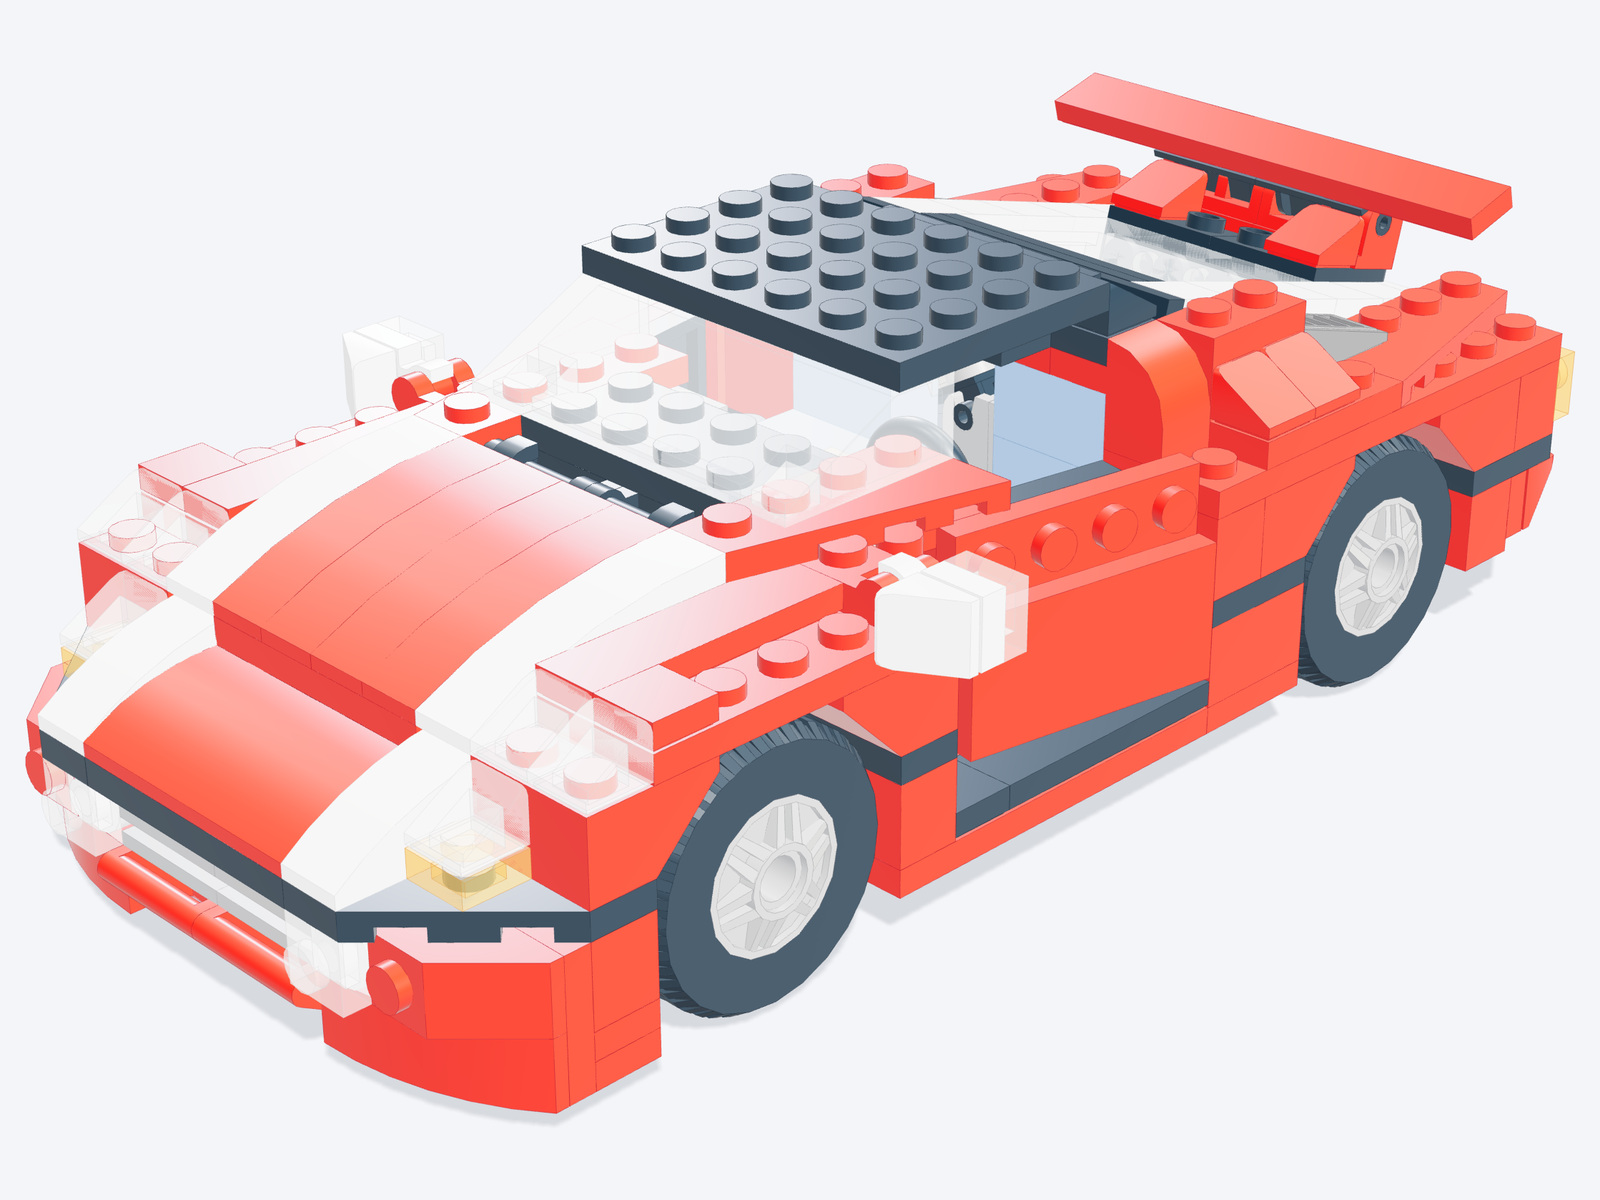
\includegraphics[width=.65\linewidth]{figures-v2/5867-iso.jpg}\end{center}
\paragraph{Attribution.}Takeshi Takahashi [RainbowDolphin]. CC BY 2.0.\par\url{https://library.ldraw.org/omr/sets/1431}
\paragraph{Source SHA256.}\path{48082e34b40a6ed5bbf2edabe9d0deb313fac7c20b1128970ba73f722b70216d}
\paragraph{Connector records.}stud: 724; axle: 32; hinge: 6; fixed: 16; ball: 0
\paragraph{Public input lock.}\path{2e851c31a59697213e445bf901ecb0e4af598ed38bb69af2aee676148e0033a1}
\paragraph{Status.}Source preservation does not certify stability. Reference outputs below are internal review material. Full model inputs are the versioned public JSON and numbered PNGs.
\begin{enumerate}
\item \textbf{ld2-5867-color-1}. Identify the original color of B0126; numbered isolation is allowed.
\par{\small color; visual; atomic; single-choice.\par\textit{Operands:} B0126 = brick\_000126\par\textit{Public evidence summary:} Numbered PNG: benchmark/ldraw-v2/inputs/views/ld2-5867-color-1.png; structured input = \{\}.\par\textit{Options:} A: Red; B: Trans Red; C: White; D: Light Bluish Grey\par\textit{Reference output:} \{"choiceId": "B"\}\par\textit{Derivation:} source colorName by rendered B-label; source oracle only\par\textit{Equivalence:} exact declared response\par\textit{Review:} pending required human review.}
\item \textbf{ld2-5867-shape-match-1}. Ignoring color and pose, which numbered instance has the same LDraw part type as B0126?
\par{\small shape-match; visual; atomic; single-choice.\par\textit{Operands:} B0126 = brick\_000126, B0113 = brick\_000113, B0067 = brick\_000067, B0268 = brick\_000268, B0011 = brick\_000011\par\textit{Public evidence summary:} Numbered PNG: benchmark/ldraw-v2/inputs/views/ld2-5867-shape-match-1.png; structured input = \{\}.\par\textit{Options:} A: B0113; B: B0011; C: B0268; D: B0067\par\textit{Reference output:} \{"choiceId": "C"\}\par\textit{Derivation:} source partNumber equality across labeled candidates; source oracle only\par\textit{Equivalence:} same source partNumber; ignore color and pose; perceptual equivalence pending\par\textit{Review:} pending required human review.}
\item \textbf{ld2-5867-distance-1}. Using the supplied geometry bounding-box centers, which candidate is nearest to B0126?
\par{\small distance; source-data; atomic; single-choice.\par\textit{Operands:} B0127 = brick\_000127, B0048 = brick\_000048, B0126 = brick\_000126, B0258 = brick\_000258\par\textit{Public evidence summary:} \{"coordinateFrame": "Viewer world, millimeters, Euclidean distance", "centers": \{"B0126": [82.4, 21.6, -28], "B0258": [-56, 30.4, 4], "B0127": [82.4, 21.6, 28], "B0048": [-80.8, 8.8, 20]\}\}\par\textit{Options:} A: B0048; B: B0127; C: B0258\par\textit{Reference output:} \{"choiceId": "B"\}\par\textit{Derivation:} Euclidean norm from public rounded centers\par\textit{Equivalence:} exact declared response\par\textit{Review:} machine checks passed; no human certification.}
\item \textbf{ld2-5867-color-2}. Identify the original color of B0232; numbered isolation is allowed.
\par{\small color; visual; atomic; single-choice.\par\textit{Operands:} B0232 = brick\_000232\par\textit{Public evidence summary:} Numbered PNG: benchmark/ldraw-v2/inputs/views/ld2-5867-color-2.png; structured input = \{\}.\par\textit{Options:} A: Light Bluish Grey; B: Dark Bluish Grey; C: Black; D: Medium Blue\par\textit{Reference output:} \{"choiceId": "C"\}\par\textit{Derivation:} source colorName by rendered B-label; source oracle only\par\textit{Equivalence:} exact declared response\par\textit{Review:} pending required human review.}
\item \textbf{ld2-5867-shape-match-2}. Ignoring color and pose, which numbered instance has the same LDraw part type as B0232?
\par{\small shape-match; visual; atomic; single-choice.\par\textit{Operands:} B0086 = brick\_000086, B0238 = brick\_000238, B0138 = brick\_000138, B0232 = brick\_000232, B0114 = brick\_000114\par\textit{Public evidence summary:} Numbered PNG: benchmark/ldraw-v2/inputs/views/ld2-5867-shape-match-2.png; structured input = \{\}.\par\textit{Options:} A: B0138; B: B0238; C: B0114; D: B0086\par\textit{Reference output:} \{"choiceId": "B"\}\par\textit{Derivation:} source partNumber equality across labeled candidates; source oracle only\par\textit{Equivalence:} same source partNumber; ignore color and pose; perceptual equivalence pending\par\textit{Review:} pending required human review.}
\item \textbf{ld2-5867-distance-2}. Using the supplied geometry bounding-box centers, which candidate is nearest to B0232?
\par{\small distance; source-data; atomic; single-choice.\par\textit{Operands:} B0079 = brick\_000079, B0205 = brick\_000205, B0232 = brick\_000232, B0020 = brick\_000020\par\textit{Public evidence summary:} \{"coordinateFrame": "Viewer world, millimeters, Euclidean distance", "centers": \{"B0232": [-7.648536, 24, 27.340845], "B0205": [-32, 21.6, -32], "B0020": [16, 8.8, -16], "B0079": [78.32, 0.8, 4]\}\}\par\textit{Options:} A: B0079; B: B0020; C: B0205\par\textit{Reference output:} \{"choiceId": "B"\}\par\textit{Derivation:} Euclidean norm from public rounded centers\par\textit{Equivalence:} exact declared response\par\textit{Review:} machine checks passed; no human certification.}
\item \textbf{ld2-5867-interface-1}. Classify the supplied connector record for B0272 and B0017. This does not certify load capacity.
\par{\small interface; connector-graph; metacognitive; single-choice.\par\textit{Operands:} B0017 = brick\_000017, B0272 = brick\_000272\par\textit{Public evidence summary:} \{"connectorRecord": \{"family": "axle", "aConnector": 0, "bConnector": 1\}, "scope": "Upstream connector tolerances and inset mesh intersections; unknown parts remain explicit, separate scene objects are not glued together; no load/force validation."\}\par\textit{Options:} A: ball; B: hinge; C: stud; D: fixed; E: axle\par\textit{Reference output:} \{"choiceId": "E"\}\par\textit{Derivation:} public connectorRecord.family equality\par\textit{Equivalence:} exact declared response\par\textit{Review:} machine checks passed; no human certification.}
\item \textbf{ld2-5867-interface-2}. Classify the supplied connector record for B0271 and B0275. This does not certify load capacity.
\par{\small interface; connector-graph; metacognitive; single-choice.\par\textit{Operands:} B0271 = brick\_000271, B0275 = brick\_000275\par\textit{Public evidence summary:} \{"connectorRecord": \{"family": "fixed", "aConnector": 2, "bConnector": 0\}, "scope": "Upstream connector tolerances and inset mesh intersections; unknown parts remain explicit, separate scene objects are not glued together; no load/force validation."\}\par\textit{Options:} A: ball; B: hinge; C: axle; D: fixed; E: stud\par\textit{Reference output:} \{"choiceId": "D"\}\par\textit{Derivation:} public connectorRecord.family equality\par\textit{Equivalence:} exact declared response\par\textit{Review:} machine checks passed; no human certification.}
\item \textbf{ld2-5867-interface-3}. Classify the supplied connector record for B0109 and B0108. This does not certify load capacity.
\par{\small interface; connector-graph; metacognitive; single-choice.\par\textit{Operands:} B0108 = brick\_000108, B0109 = brick\_000109\par\textit{Public evidence summary:} \{"connectorRecord": \{"family": "hinge", "aConnector": 6, "bConnector": 2\}, "scope": "Upstream connector tolerances and inset mesh intersections; unknown parts remain explicit, separate scene objects are not glued together; no load/force validation."\}\par\textit{Options:} A: ball; B: stud; C: hinge; D: fixed; E: axle\par\textit{Reference output:} \{"choiceId": "C"\}\par\textit{Derivation:} public connectorRecord.family equality\par\textit{Equivalence:} exact declared response\par\textit{Review:} machine checks passed; no human certification.}
\item \textbf{ld2-5867-interface-4}. Classify the supplied connector record for B0011 and B0033. This does not certify load capacity.
\par{\small interface; connector-graph; metacognitive; single-choice.\par\textit{Operands:} B0033 = brick\_000033, B0011 = brick\_000011\par\textit{Public evidence summary:} \{"connectorRecord": \{"family": "stud", "aConnector": 38, "bConnector": 3\}, "scope": "Upstream connector tolerances and inset mesh intersections; unknown parts remain explicit, separate scene objects are not glued together; no load/force validation."\}\par\textit{Options:} A: ball; B: stud; C: hinge; D: axle; E: fixed\par\textit{Reference output:} \{"choiceId": "B"\}\par\textit{Derivation:} public connectorRecord.family equality\par\textit{Equivalence:} exact declared response\par\textit{Review:} machine checks passed; no human certification.}
\item \textbf{ld2-5867-neighbors-1}. Select every candidate directly adjacent to B0202 in the supplied connector graph.
\par{\small neighbors; connector-graph; metacognitive; multiple-choice.\par\textit{Operands:} B0245 = brick\_000245, B0069 = brick\_000069, B0021 = brick\_000021, B0202 = brick\_000202, B0215 = brick\_000215, B0244 = brick\_000244, B0056 = brick\_000056\par\textit{Public evidence summary:} 4 unique undirected pairs\par\textit{Options:} A: B0056; B: B0069; C: B0245; D: B0244; E: B0021; F: B0215\par\textit{Reference output:} \{"choiceIds": ["B", "C", "D", "F"]\}\par\textit{Derivation:} public incident edge endpoint set\par\textit{Equivalence:} unordered exact set; duplicate IDs invalid\par\textit{Review:} machine checks passed; no human certification.}
\item \textbf{ld2-5867-graph-removal-1}. Delete B0202 and its incident edges from this local graph. How many connected components remain? Do not infer physical extractability.
\par{\small graph-removal; connector-graph; graph-internal; integer.\par\textit{Operands:} B0056 = brick\_000056, B0202 = brick\_000202, B0215 = brick\_000215, B0021 = brick\_000021, B0069 = brick\_000069, B0244 = brick\_000244, B0245 = brick\_000245\par\textit{Public evidence summary:} 4 unique undirected pairs; 7 nodes\par\textit{Reference output:} \{"value": 6\}\par\textit{Derivation:} union-find component count after public target deletion\par\textit{Equivalence:} exact declared response\par\textit{Review:} machine checks passed; no human certification.}
\item \textbf{ld2-5867-neighbors-2}. Select every candidate directly adjacent to B0193 in the supplied connector graph.
\par{\small neighbors; connector-graph; metacognitive; multiple-choice.\par\textit{Operands:} B0228 = brick\_000228, B0197 = brick\_000197, B0193 = brick\_000193, B0187 = brick\_000187, B0031 = brick\_000031, B0196 = brick\_000196\par\textit{Public evidence summary:} 3 unique undirected pairs\par\textit{Options:} A: B0031; B: B0197; C: B0187; D: B0196; E: B0228\par\textit{Reference output:} \{"choiceIds": ["C", "D", "E"]\}\par\textit{Derivation:} public incident edge endpoint set\par\textit{Equivalence:} unordered exact set; duplicate IDs invalid\par\textit{Review:} machine checks passed; no human certification.}
\item \textbf{ld2-5867-graph-removal-2}. Delete B0193 and its incident edges from this local graph. How many connected components remain? Do not infer physical extractability.
\par{\small graph-removal; connector-graph; graph-internal; integer.\par\textit{Operands:} B0196 = brick\_000196, B0187 = brick\_000187, B0228 = brick\_000228, B0031 = brick\_000031, B0197 = brick\_000197, B0193 = brick\_000193\par\textit{Public evidence summary:} 3 unique undirected pairs; 6 nodes\par\textit{Reference output:} \{"value": 5\}\par\textit{Derivation:} union-find component count after public target deletion\par\textit{Equivalence:} exact declared response\par\textit{Review:} machine checks passed; no human certification.}
\item \textbf{ld2-5867-coverage-1}. Which numbered instance lacks a connector definition in the coverage record, so this audit cannot establish that it is floating?
\par{\small coverage; source-data; metacognitive; single-choice.\par\textit{Operands:} B0232 = brick\_000232, B0194 = brick\_000194, B0126 = brick\_000126, B0109 = brick\_000109\par\textit{Public evidence summary:} \{"coverage": [\{"label": "B0194", "supported": false\}, \{"label": "B0126", "supported": true\}, \{"label": "B0232", "supported": true\}, \{"label": "B0109", "supported": true\}]\}\par\textit{Options:} A: B0109; B: B0126; C: B0194; D: B0232\par\textit{Reference output:} \{"choiceId": "C"\}\par\textit{Derivation:} public supported=false record\par\textit{Equivalence:} exact declared response\par\textit{Review:} pending required human review.}
\item \textbf{ld2-5867-evidence-limit-1}. Only source geometry, connector matching and mesh intersection audits are available. Without mass, friction, material or dynamic tests, is gravitational stability established?
\par{\small evidence-limit; source-data; metacognitive; single-choice.\par\textit{Operands:} none\par\textit{Public evidence summary:} \{"available": ["Original CAD", "Connector inference", "Inset-mesh intersection candidates"]\}\par\textit{Options:} A: Not established by this evidence; B: Established\par\textit{Reference output:} \{"choiceId": "A"\}\par\textit{Derivation:} fixed epistemic control label\par\textit{Equivalence:} exact declared response\par\textit{Review:} machine checks passed; no human certification.}
\item \textbf{ld2-5867-restore-instance-1}. The display copy hides B0126. Restore only that numbered instance, preserving all other instances and source poses.
\par{\small restore-instance; scene-edit; procedural; actions.\par\textit{Operands:} B0001 = brick\_000001, B0126 = brick\_000126\par\textit{Public evidence summary:} 2 public actions; budget 1; \{"initialFacts": ["missing-brick\_000126", "present-brick\_000001"], "goalFacts": ["present-brick\_000126", "present-brick\_000001"], "absentFacts": ["missing-brick\_000126"]\}\par\textit{Reference output:} \{"actionIds": ["restore-B0126"]\}\par\textit{Derivation:} public precondition solver\par\textit{Equivalence:} any legal sequence reaching all goals within budget; display-only semantics\par\textit{Review:} machine checks passed; no human certification.}
\item \textbf{ld2-5867-restore-instance-2}. The display copy hides B0232. Restore only that numbered instance, preserving all other instances and source poses.
\par{\small restore-instance; scene-edit; procedural; actions.\par\textit{Operands:} B0001 = brick\_000001, B0232 = brick\_000232\par\textit{Public evidence summary:} 2 public actions; budget 1; \{"initialFacts": ["missing-brick\_000232", "present-brick\_000001"], "goalFacts": ["present-brick\_000232", "present-brick\_000001"], "absentFacts": ["missing-brick\_000232"]\}\par\textit{Reference output:} \{"actionIds": ["restore-B0232"]\}\par\textit{Derivation:} public precondition solver\par\textit{Equivalence:} any legal sequence reaching all goals within budget; display-only semantics\par\textit{Review:} machine checks passed; no human certification.}
\end{enumerate}
\clearpage\section{10128: Train Level Crossing}
336 source instances; 21 tasks; D2 size band. 111 type strings; 17 color codes; 2 unsupported instances; 1 intersection candidates. 87 expanded author steps. Independent reparse: passed.
\begin{center}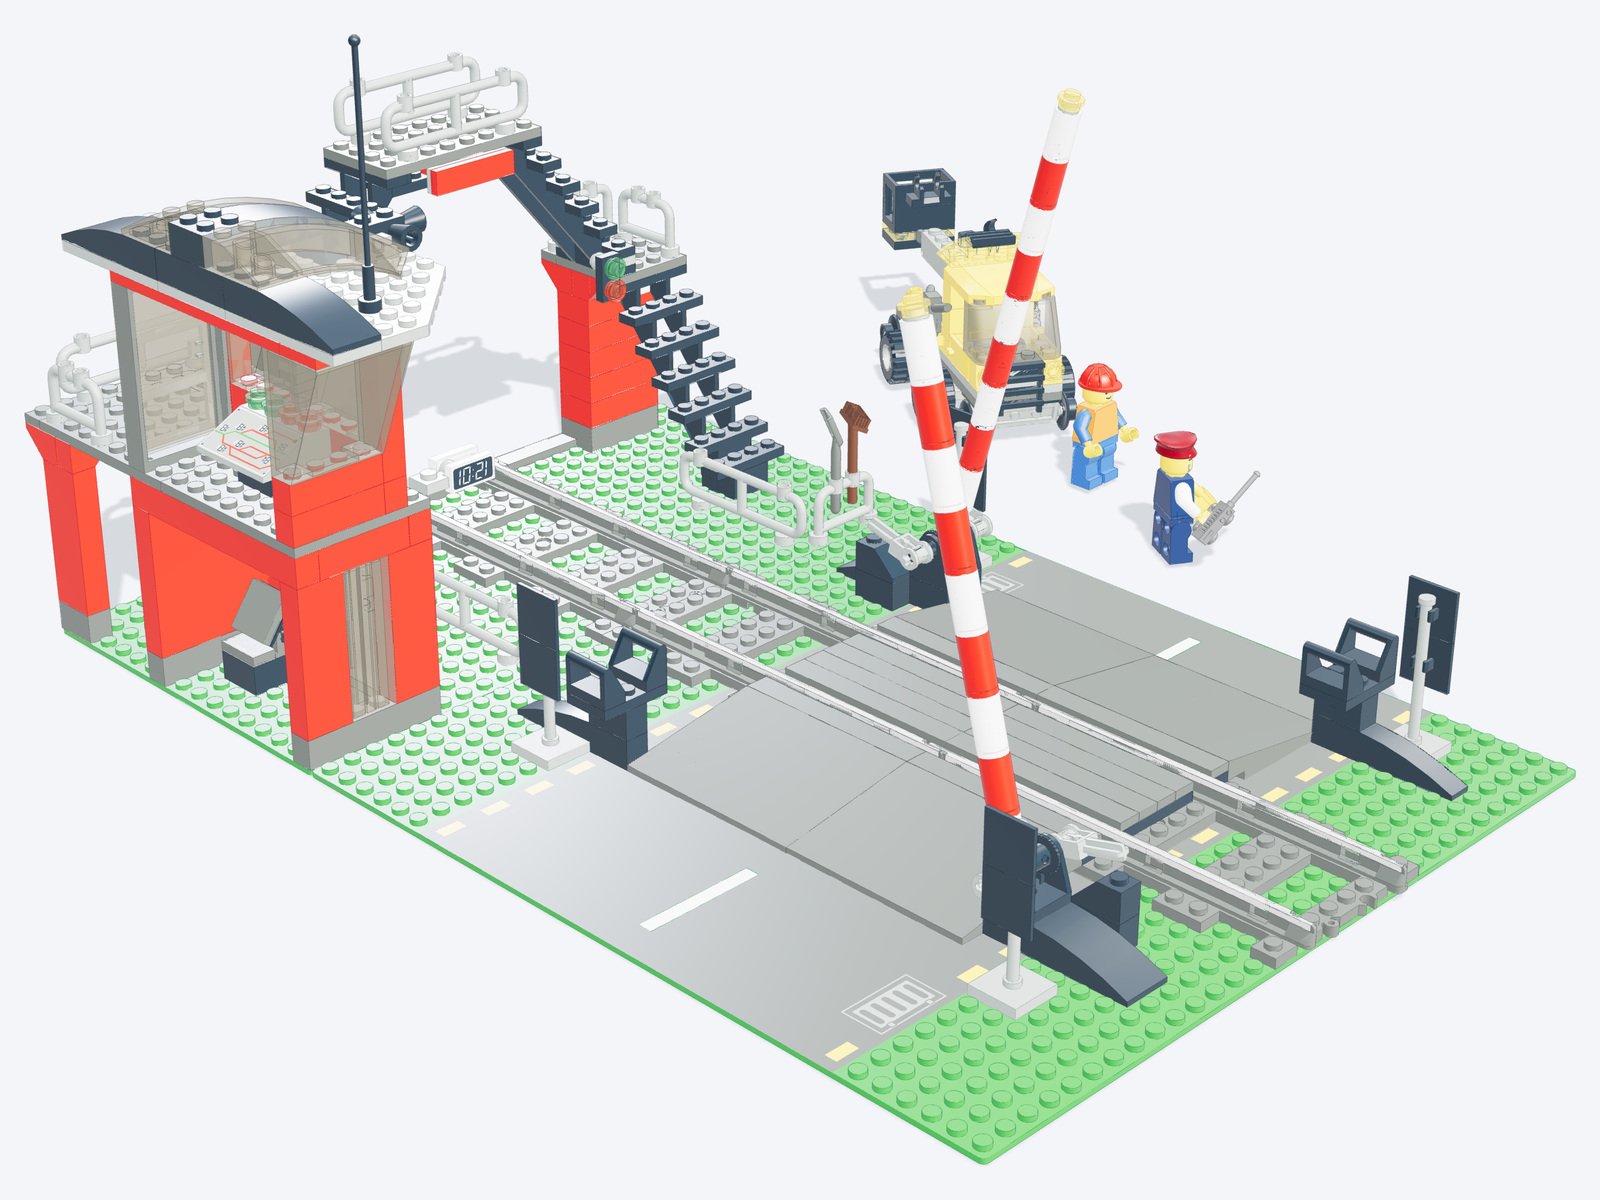
\includegraphics[width=.65\linewidth]{figures-v2/10128-iso.jpg}\end{center}
\paragraph{Attribution.}Robert Paciorek [bercik]. CC BY 2.0.\par\url{https://library.ldraw.org/omr/sets/864}
\paragraph{Source SHA256.}\path{7928f4e259455ec49cc02c62acb1653f7a002824c789f099845936d0a2e8a0b9}
\paragraph{Connector records.}stud: 963; axle: 89; hinge: 23; fixed: 20; ball: 0
\paragraph{Public input lock.}\path{8bbe24f7936ea6cea2aea8fc7e4c0d3de2c086e4760a9f22631139beee0104e1}
\paragraph{Status.}Source preservation does not certify stability. Reference outputs below are internal review material. Full model inputs are the versioned public JSON and numbered PNGs.
\begin{enumerate}
\item \textbf{ld2-10128-color-1}. Identify the original color of B0075; numbered isolation is allowed.
\par{\small color; visual; atomic; single-choice.\par\textit{Operands:} B0075 = brick\_000075\par\textit{Public evidence summary:} Numbered PNG: benchmark/ldraw-v2/inputs/views/ld2-10128-color-1.png; structured input = \{\}.\par\textit{Options:} A: Blue; B: Trans Brown; C: Dark Blue; D: Dark Grey\par\textit{Reference output:} \{"choiceId": "D"\}\par\textit{Derivation:} source colorName by rendered B-label; source oracle only\par\textit{Equivalence:} exact declared response\par\textit{Review:} pending required human review.}
\item \textbf{ld2-10128-shape-match-1}. Ignoring color and pose, which numbered instance has the same LDraw part type as B0075?
\par{\small shape-match; visual; atomic; single-choice.\par\textit{Operands:} B0075 = brick\_000075, B0313 = brick\_000313, B0248 = brick\_000248, B0125 = brick\_000125, B0037 = brick\_000037\par\textit{Public evidence summary:} Numbered PNG: benchmark/ldraw-v2/inputs/views/ld2-10128-shape-match-1.png; structured input = \{\}.\par\textit{Options:} A: B0125; B: B0037; C: B0248; D: B0313\par\textit{Reference output:} \{"choiceId": "B"\}\par\textit{Derivation:} source partNumber equality across labeled candidates; source oracle only\par\textit{Equivalence:} same source partNumber; ignore color and pose; perceptual equivalence pending\par\textit{Review:} pending required human review.}
\item \textbf{ld2-10128-distance-1}. Using the supplied geometry bounding-box centers, which candidate is nearest to B0075?
\par{\small distance; source-data; atomic; single-choice.\par\textit{Operands:} B0310 = brick\_000310, B0105 = brick\_000105, B0031 = brick\_000031, B0075 = brick\_000075\par\textit{Public evidence summary:} \{"coordinateFrame": "Viewer world, millimeters, Euclidean distance", "centers": \{"B0075": [-72, 100, -60], "B0105": [-80, 133.6, 16], "B0310": [226.2552, 10.4, -29.7924], "B0031": [-44, 5.6, -28]\}\}\par\textit{Options:} A: B0031; B: B0310; C: B0105\par\textit{Reference output:} \{"choiceId": "C"\}\par\textit{Derivation:} Euclidean norm from public rounded centers\par\textit{Equivalence:} exact declared response\par\textit{Review:} machine checks passed; no human certification.}
\item \textbf{ld2-10128-color-2}. Identify the original color of B0129; numbered isolation is allowed.
\par{\small color; visual; atomic; single-choice.\par\textit{Operands:} B0129 = brick\_000129\par\textit{Public evidence summary:} Numbered PNG: benchmark/ldraw-v2/inputs/views/ld2-10128-color-2.png; structured input = \{\}.\par\textit{Options:} A: Green; B: Dark Red; C: Light Grey; D: Trans Red\par\textit{Reference output:} \{"choiceId": "C"\}\par\textit{Derivation:} source colorName by rendered B-label; source oracle only\par\textit{Equivalence:} exact declared response\par\textit{Review:} pending required human review.}
\item \textbf{ld2-10128-shape-match-2}. Ignoring color and pose, which numbered instance has the same LDraw part type as B0129?
\par{\small shape-match; visual; atomic; single-choice.\par\textit{Operands:} B0129 = brick\_000129, B0145 = brick\_000145, B0074 = brick\_000074, B0161 = brick\_000161, B0144 = brick\_000144\par\textit{Public evidence summary:} Numbered PNG: benchmark/ldraw-v2/inputs/views/ld2-10128-shape-match-2.png; structured input = \{\}.\par\textit{Options:} A: B0074; B: B0161; C: B0144; D: B0145\par\textit{Reference output:} \{"choiceId": "A"\}\par\textit{Derivation:} source partNumber equality across labeled candidates; source oracle only\par\textit{Equivalence:} same source partNumber; ignore color and pose; perceptual equivalence pending\par\textit{Review:} pending required human review.}
\item \textbf{ld2-10128-distance-2}. Using the supplied geometry bounding-box centers, which candidate is nearest to B0129?
\par{\small distance; source-data; atomic; single-choice.\par\textit{Operands:} B0095 = brick\_000095, B0082 = brick\_000082, B0141 = brick\_000141, B0129 = brick\_000129\par\textit{Public evidence summary:} \{"coordinateFrame": "Viewer world, millimeters, Euclidean distance", "centers": \{"B0129": [56, 141.6, -108], "B0141": [24, 2.4, 96], "B0082": [120.4, 76, -84], "B0095": [-52, 104.8, 12]\}\}\par\textit{Options:} A: B0082; B: B0141; C: B0095\par\textit{Reference output:} \{"choiceId": "A"\}\par\textit{Derivation:} Euclidean norm from public rounded centers\par\textit{Equivalence:} exact declared response\par\textit{Review:} machine checks passed; no human certification.}
\item \textbf{ld2-10128-interface-1}. Classify the supplied connector record for B0260 and B0251. This does not certify load capacity.
\par{\small interface; connector-graph; metacognitive; single-choice.\par\textit{Operands:} B0260 = brick\_000260, B0251 = brick\_000251\par\textit{Public evidence summary:} \{"connectorRecord": \{"family": "axle", "aConnector": 1, "bConnector": 0\}, "scope": "Upstream connector tolerances and inset mesh intersections; unknown parts remain explicit, separate scene objects are not glued together; no load/force validation."\}\par\textit{Options:} A: axle; B: fixed; C: hinge; D: ball; E: stud\par\textit{Reference output:} \{"choiceId": "A"\}\par\textit{Derivation:} public connectorRecord.family equality\par\textit{Equivalence:} exact declared response\par\textit{Review:} machine checks passed; no human certification.}
\item \textbf{ld2-10128-interface-2}. Classify the supplied connector record for B0327 and B0326. This does not certify load capacity.
\par{\small interface; connector-graph; metacognitive; single-choice.\par\textit{Operands:} B0327 = brick\_000327, B0326 = brick\_000326\par\textit{Public evidence summary:} \{"connectorRecord": \{"family": "fixed", "aConnector": 0, "bConnector": 2\}, "scope": "Upstream connector tolerances and inset mesh intersections; unknown parts remain explicit, separate scene objects are not glued together; no load/force validation."\}\par\textit{Options:} A: stud; B: axle; C: fixed; D: ball; E: hinge\par\textit{Reference output:} \{"choiceId": "C"\}\par\textit{Derivation:} public connectorRecord.family equality\par\textit{Equivalence:} exact declared response\par\textit{Review:} machine checks passed; no human certification.}
\item \textbf{ld2-10128-interface-3}. Classify the supplied connector record for B0328 and B0326. This does not certify load capacity.
\par{\small interface; connector-graph; metacognitive; single-choice.\par\textit{Operands:} B0326 = brick\_000326, B0328 = brick\_000328\par\textit{Public evidence summary:} \{"connectorRecord": \{"family": "hinge", "aConnector": 0, "bConnector": 6\}, "scope": "Upstream connector tolerances and inset mesh intersections; unknown parts remain explicit, separate scene objects are not glued together; no load/force validation."\}\par\textit{Options:} A: ball; B: fixed; C: axle; D: stud; E: hinge\par\textit{Reference output:} \{"choiceId": "E"\}\par\textit{Derivation:} public connectorRecord.family equality\par\textit{Equivalence:} exact declared response\par\textit{Review:} machine checks passed; no human certification.}
\item \textbf{ld2-10128-interface-4}. Classify the supplied connector record for B0249 and B0270. This does not certify load capacity.
\par{\small interface; connector-graph; metacognitive; single-choice.\par\textit{Operands:} B0249 = brick\_000249, B0270 = brick\_000270\par\textit{Public evidence summary:} \{"connectorRecord": \{"family": "stud", "aConnector": 84, "bConnector": 5\}, "scope": "Upstream connector tolerances and inset mesh intersections; unknown parts remain explicit, separate scene objects are not glued together; no load/force validation."\}\par\textit{Options:} A: hinge; B: fixed; C: ball; D: axle; E: stud\par\textit{Reference output:} \{"choiceId": "E"\}\par\textit{Derivation:} public connectorRecord.family equality\par\textit{Equivalence:} exact declared response\par\textit{Review:} machine checks passed; no human certification.}
\item \textbf{ld2-10128-neighbors-1}. Select every candidate directly adjacent to B0188 in the supplied connector graph.
\par{\small neighbors; connector-graph; metacognitive; multiple-choice.\par\textit{Operands:} B0199 = brick\_000199, B0139 = brick\_000139, B0055 = brick\_000055, B0190 = brick\_000190, B0188 = brick\_000188\par\textit{Public evidence summary:} 2 unique undirected pairs\par\textit{Options:} A: B0199; B: B0190; C: B0055; D: B0139\par\textit{Reference output:} \{"choiceIds": ["B", "D"]\}\par\textit{Derivation:} public incident edge endpoint set\par\textit{Equivalence:} unordered exact set; duplicate IDs invalid\par\textit{Review:} machine checks passed; no human certification.}
\item \textbf{ld2-10128-graph-removal-1}. Delete B0188 and its incident edges from this local graph. How many connected components remain? Do not infer physical extractability.
\par{\small graph-removal; connector-graph; graph-internal; integer.\par\textit{Operands:} B0188 = brick\_000188, B0055 = brick\_000055, B0190 = brick\_000190, B0139 = brick\_000139, B0199 = brick\_000199\par\textit{Public evidence summary:} 2 unique undirected pairs; 5 nodes\par\textit{Reference output:} \{"value": 4\}\par\textit{Derivation:} union-find component count after public target deletion\par\textit{Equivalence:} exact declared response\par\textit{Review:} machine checks passed; no human certification.}
\item \textbf{ld2-10128-neighbors-2}. Select every candidate directly adjacent to B0163 in the supplied connector graph.
\par{\small neighbors; connector-graph; metacognitive; multiple-choice.\par\textit{Operands:} B0154 = brick\_000154, B0163 = brick\_000163, B0165 = brick\_000165, B0148 = brick\_000148, B0242 = brick\_000242\par\textit{Public evidence summary:} 4 unique undirected pairs\par\textit{Options:} A: B0165; B: B0154; C: B0148; D: B0242\par\textit{Reference output:} \{"choiceIds": ["B", "C"]\}\par\textit{Derivation:} public incident edge endpoint set\par\textit{Equivalence:} unordered exact set; duplicate IDs invalid\par\textit{Review:} machine checks passed; no human certification.}
\item \textbf{ld2-10128-graph-removal-2}. Delete B0163 and its incident edges from this local graph. How many connected components remain? Do not infer physical extractability.
\par{\small graph-removal; connector-graph; graph-internal; integer.\par\textit{Operands:} B0242 = brick\_000242, B0165 = brick\_000165, B0154 = brick\_000154, B0163 = brick\_000163, B0148 = brick\_000148\par\textit{Public evidence summary:} 4 unique undirected pairs; 5 nodes\par\textit{Reference output:} \{"value": 2\}\par\textit{Derivation:} union-find component count after public target deletion\par\textit{Equivalence:} exact declared response\par\textit{Review:} machine checks passed; no human certification.}
\item \textbf{ld2-10128-coverage-1}. Which numbered instance lacks a connector definition in the coverage record, so this audit cannot establish that it is floating?
\par{\small coverage; source-data; metacognitive; single-choice.\par\textit{Operands:} B0038 = brick\_000038, B0128 = brick\_000128, B0129 = brick\_000129, B0075 = brick\_000075\par\textit{Public evidence summary:} \{"coverage": [\{"label": "B0038", "supported": false\}, \{"label": "B0129", "supported": true\}, \{"label": "B0075", "supported": true\}, \{"label": "B0128", "supported": true\}]\}\par\textit{Options:} A: B0129; B: B0038; C: B0128; D: B0075\par\textit{Reference output:} \{"choiceId": "B"\}\par\textit{Derivation:} public supported=false record\par\textit{Equivalence:} exact declared response\par\textit{Review:} pending required human review.}
\item \textbf{ld2-10128-evidence-limit-1}. Only source geometry, connector matching and mesh intersection audits are available. Without mass, friction, material or dynamic tests, is gravitational stability established?
\par{\small evidence-limit; source-data; metacognitive; single-choice.\par\textit{Operands:} none\par\textit{Public evidence summary:} \{"available": ["Original CAD", "Connector inference", "Inset-mesh intersection candidates"]\}\par\textit{Options:} A: Established; B: Not established by this evidence\par\textit{Reference output:} \{"choiceId": "B"\}\par\textit{Derivation:} fixed epistemic control label\par\textit{Equivalence:} exact declared response\par\textit{Review:} machine checks passed; no human certification.}
\item \textbf{ld2-10128-source-step-1}. At which expanded author step does B0189 first appear in the supplied source-step table? Source order is not a collision-free assembly proof.
\par{\small source-step; source-data; procedural; single-choice.\par\textit{Operands:} B0001 = brick\_000001, B0189 = brick\_000189\par\textit{Public evidence summary:} 2 supplied author-step records; exact table in public JSON\par\textit{Options:} A: 65; B: 40; C: 13; D: 18\par\textit{Reference output:} \{"choiceId": "B"\}\par\textit{Derivation:} minimum public step index containing target\par\textit{Equivalence:} exact declared response\par\textit{Review:} machine checks passed; no human certification.}
\item \textbf{ld2-10128-source-step-2}. At which expanded author step does B0297 first appear in the supplied source-step table? Source order is not a collision-free assembly proof.
\par{\small source-step; source-data; procedural; single-choice.\par\textit{Operands:} B0297 = brick\_000297, B0001 = brick\_000001\par\textit{Public evidence summary:} 2 supplied author-step records; exact table in public JSON\par\textit{Options:} A: 80; B: 6; C: 63; D: 81\par\textit{Reference output:} \{"choiceId": "A"\}\par\textit{Derivation:} minimum public step index containing target\par\textit{Equivalence:} exact declared response\par\textit{Review:} machine checks passed; no human certification.}
\item \textbf{ld2-10128-source-sequence-1}. Reveal the supplied source-step window in author order. Actions change visibility only, without simulating insertion trajectories.
\par{\small source-sequence; scene-edit; procedural; actions.\par\textit{Operands:} B0021 = brick\_000021, B0002 = brick\_000002, B0009 = brick\_000009, B0012 = brick\_000012, B0005 = brick\_000005, B0018 = brick\_000018, B0023 = brick\_000023, B0022 = brick\_000022, B0003 = brick\_000003, B0013 = brick\_000013, B0014 = brick\_000014, B0024 = brick\_000024, B0016 = brick\_000016, B0010 = brick\_000010, B0001 = brick\_000001, B0004 = brick\_000004, B0006 = brick\_000006, B0019 = brick\_000019, B0007 = brick\_000007, B0011 = brick\_000011, B0020 = brick\_000020, B0017 = brick\_000017, B0015 = brick\_000015, B0008 = brick\_000008\par\textit{Public evidence summary:} 6 public actions; budget 6; \{"initialFacts": ["start"], "goalFacts": ["done-6"], "absentFacts": []\}\par\textit{Reference output:} \{"actionIds": ["step-1", "step-2", "step-3", "step-4", "step-5", "step-6"]\}\par\textit{Derivation:} public precondition solver\par\textit{Equivalence:} any legal sequence reaching all goals within budget; display-only semantics\par\textit{Review:} machine checks passed; no human certification.}
\item \textbf{ld2-10128-restore-instance-1}. The display copy hides B0075. Restore only that numbered instance, preserving all other instances and source poses.
\par{\small restore-instance; scene-edit; procedural; actions.\par\textit{Operands:} B0001 = brick\_000001, B0075 = brick\_000075\par\textit{Public evidence summary:} 2 public actions; budget 1; \{"initialFacts": ["missing-brick\_000075", "present-brick\_000001"], "goalFacts": ["present-brick\_000075", "present-brick\_000001"], "absentFacts": ["missing-brick\_000075"]\}\par\textit{Reference output:} \{"actionIds": ["restore-B0075"]\}\par\textit{Derivation:} public precondition solver\par\textit{Equivalence:} any legal sequence reaching all goals within budget; display-only semantics\par\textit{Review:} machine checks passed; no human certification.}
\item \textbf{ld2-10128-restore-instance-2}. The display copy hides B0129. Restore only that numbered instance, preserving all other instances and source poses.
\par{\small restore-instance; scene-edit; procedural; actions.\par\textit{Operands:} B0129 = brick\_000129, B0001 = brick\_000001\par\textit{Public evidence summary:} 2 public actions; budget 1; \{"initialFacts": ["missing-brick\_000129", "present-brick\_000001"], "goalFacts": ["present-brick\_000129", "present-brick\_000001"], "absentFacts": ["missing-brick\_000129"]\}\par\textit{Reference output:} \{"actionIds": ["restore-B0129"]\}\par\textit{Derivation:} public precondition solver\par\textit{Equivalence:} any legal sequence reaching all goals within budget; display-only semantics\par\textit{Review:} machine checks passed; no human certification.}
\end{enumerate}
\clearpage\section{10159: City Airport}
592 source instances; 25 tasks; D3 size band. 160 type strings; 14 color codes; 30 unsupported instances; 26 intersection candidates. 0 expanded author steps. Independent reparse: passed.
\begin{center}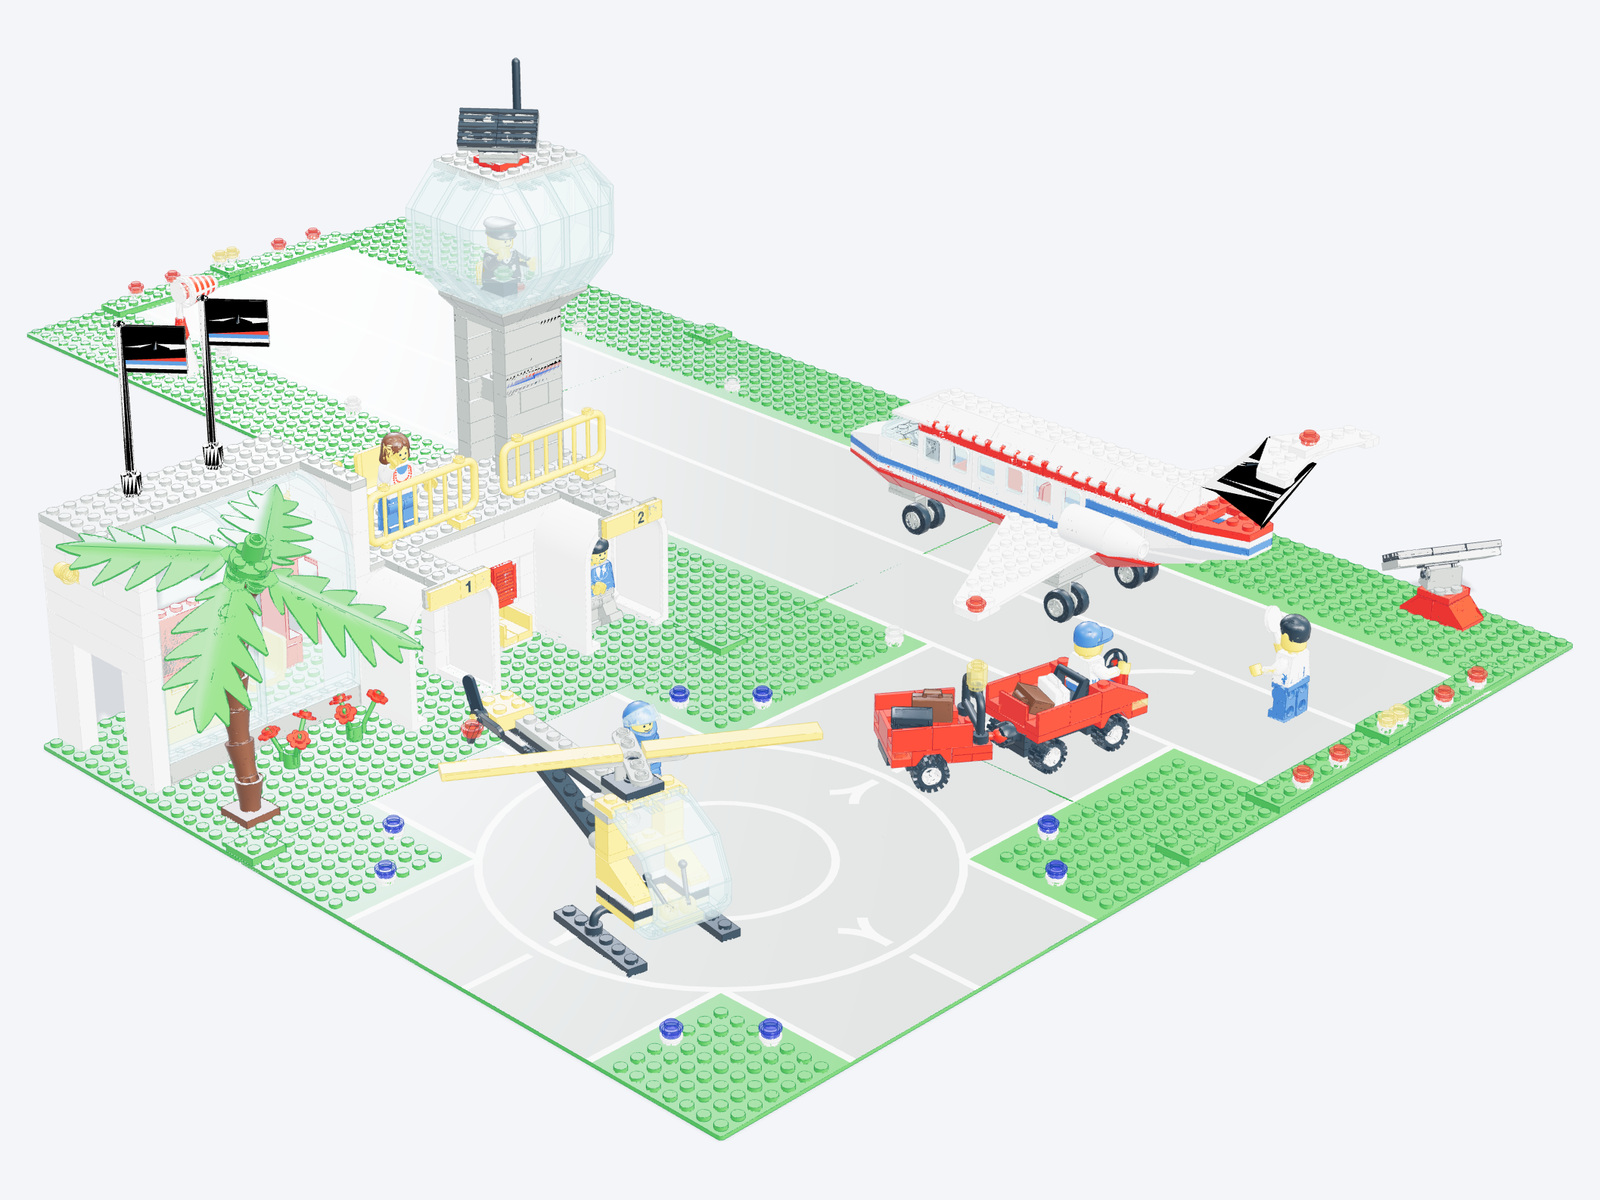
\includegraphics[width=.65\linewidth]{figures-v2/10159-iso.jpg}\end{center}
\paragraph{Attribution.}Zoltan Keri [kzoltan82]. CC BY 2.0.\par\url{https://library.ldraw.org/omr/sets/660}
\paragraph{Source SHA256.}\path{ef0b08af1e69059813e8965d3aa8fdd6a4aadbb04a21d92723cc4f9ae26bc1ec}
\paragraph{Connector records.}stud: 1109; axle: 31; hinge: 76; fixed: 62; ball: 1
\paragraph{Public input lock.}\path{47fdd0a148a08b129d77bd41f06ab35dca4bb74db3c43da8359e585139153494}
\paragraph{Status.}Source preservation does not certify stability. Reference outputs below are internal review material. Full model inputs are the versioned public JSON and numbered PNGs.
\begin{enumerate}
\item \textbf{ld2-10159-color-1}. Identify the original color of B0132; numbered isolation is allowed.
\par{\small color; visual; atomic; single-choice.\par\textit{Operands:} B0132 = brick\_000132\par\textit{Public evidence summary:} Numbered PNG: benchmark/ldraw-v2/inputs/views/ld2-10159-color-1.png; structured input = \{\}.\par\textit{Options:} A: Black; B: Brown; C: Green; D: White\par\textit{Reference output:} \{"choiceId": "D"\}\par\textit{Derivation:} source colorName by rendered B-label; source oracle only\par\textit{Equivalence:} exact declared response\par\textit{Review:} pending required human review.}
\item \textbf{ld2-10159-shape-match-1}. Ignoring color and pose, which numbered instance has the same LDraw part type as B0132?
\par{\small shape-match; visual; atomic; single-choice.\par\textit{Operands:} B0332 = brick\_000332, B0374 = brick\_000374, B0131 = brick\_000131, B0354 = brick\_000354, B0132 = brick\_000132\par\textit{Public evidence summary:} Numbered PNG: benchmark/ldraw-v2/inputs/views/ld2-10159-shape-match-1.png; structured input = \{\}.\par\textit{Options:} A: B0332; B: B0374; C: B0354; D: B0131\par\textit{Reference output:} \{"choiceId": "D"\}\par\textit{Derivation:} source partNumber equality across labeled candidates; source oracle only\par\textit{Equivalence:} same source partNumber; ignore color and pose; perceptual equivalence pending\par\textit{Review:} pending required human review.}
\item \textbf{ld2-10159-distance-1}. Using the supplied geometry bounding-box centers, which candidate is nearest to B0132?
\par{\small distance; source-data; atomic; single-choice.\par\textit{Operands:} B0510 = brick\_000510, B0234 = brick\_000234, B0132 = brick\_000132, B0138 = brick\_000138\par\textit{Public evidence summary:} \{"coordinateFrame": "Viewer world, millimeters, Euclidean distance", "centers": \{"B0132": [124, 53.6, -224], "B0234": [93.534, 213.4228, -211.256], "B0138": [-116, 53.6, -224], "B0510": [255.005523, 23.458353, 71.775633]\}\}\par\textit{Options:} A: B0234; B: B0510; C: B0138\par\textit{Reference output:} \{"choiceId": "A"\}\par\textit{Derivation:} Euclidean norm from public rounded centers\par\textit{Equivalence:} exact declared response\par\textit{Review:} machine checks passed; no human certification.}
\item \textbf{ld2-10159-color-2}. Identify the original color of B0181; numbered isolation is allowed.
\par{\small color; visual; atomic; single-choice.\par\textit{Operands:} B0181 = brick\_000181\par\textit{Public evidence summary:} Numbered PNG: benchmark/ldraw-v2/inputs/views/ld2-10159-color-2.png; structured input = \{\}.\par\textit{Options:} A: Trans Yellow; B: Blue; C: Trans Light Blue; D: Light Grey\par\textit{Reference output:} \{"choiceId": "A"\}\par\textit{Derivation:} source colorName by rendered B-label; source oracle only\par\textit{Equivalence:} exact declared response\par\textit{Review:} pending required human review.}
\item \textbf{ld2-10159-shape-match-2}. Ignoring color and pose, which numbered instance has the same LDraw part type as B0181?
\par{\small shape-match; visual; atomic; single-choice.\par\textit{Operands:} B0181 = brick\_000181, B0356 = brick\_000356, B0367 = brick\_000367, B0530 = brick\_000530, B0380 = brick\_000380\par\textit{Public evidence summary:} Numbered PNG: benchmark/ldraw-v2/inputs/views/ld2-10159-shape-match-2.png; structured input = \{\}.\par\textit{Options:} A: B0380; B: B0356; C: B0530; D: B0367\par\textit{Reference output:} \{"choiceId": "A"\}\par\textit{Derivation:} source partNumber equality across labeled candidates; source oracle only\par\textit{Equivalence:} same source partNumber; ignore color and pose; perceptual equivalence pending\par\textit{Review:} pending required human review.}
\item \textbf{ld2-10159-distance-2}. Using the supplied geometry bounding-box centers, which candidate is nearest to B0181?
\par{\small distance; source-data; atomic; single-choice.\par\textit{Operands:} B0228 = brick\_000228, B0181 = brick\_000181, B0297 = brick\_000297, B0245 = brick\_000245\par\textit{Public evidence summary:} \{"coordinateFrame": "Viewer world, millimeters, Euclidean distance", "centers": \{"B0181": [-4, 82.4, -232], "B0297": [288, 36, -48], "B0245": [-43.4404, 15.721947, -167.7786], "B0228": [96, 200, -224]\}\}\par\textit{Options:} A: B0297; B: B0228; C: B0245\par\textit{Reference output:} \{"choiceId": "C"\}\par\textit{Derivation:} Euclidean norm from public rounded centers\par\textit{Equivalence:} exact declared response\par\textit{Review:} machine checks passed; no human certification.}
\item \textbf{ld2-10159-color-3}. Identify the original color of B0485; numbered isolation is allowed.
\par{\small color; visual; atomic; single-choice.\par\textit{Operands:} B0485 = brick\_000485\par\textit{Public evidence summary:} Numbered PNG: benchmark/ldraw-v2/inputs/views/ld2-10159-color-3.png; structured input = \{\}.\par\textit{Options:} A: Trans Red; B: Light Grey; C: Yellow; D: Red\par\textit{Reference output:} \{"choiceId": "D"\}\par\textit{Derivation:} source colorName by rendered B-label; source oracle only\par\textit{Equivalence:} exact declared response\par\textit{Review:} pending required human review.}
\item \textbf{ld2-10159-shape-match-3}. Ignoring color and pose, which numbered instance has the same LDraw part type as B0485?
\par{\small shape-match; visual; atomic; single-choice.\par\textit{Operands:} B0254 = brick\_000254, B0555 = brick\_000555, B0250 = brick\_000250, B0425 = brick\_000425, B0485 = brick\_000485\par\textit{Public evidence summary:} Numbered PNG: benchmark/ldraw-v2/inputs/views/ld2-10159-shape-match-3.png; structured input = \{\}.\par\textit{Options:} A: B0254; B: B0425; C: B0555; D: B0250\par\textit{Reference output:} \{"choiceId": "B"\}\par\textit{Derivation:} source partNumber equality across labeled candidates; source oracle only\par\textit{Equivalence:} same source partNumber; ignore color and pose; perceptual equivalence pending\par\textit{Review:} pending required human review.}
\item \textbf{ld2-10159-distance-3}. Using the supplied geometry bounding-box centers, which candidate is nearest to B0485?
\par{\small distance; source-data; atomic; single-choice.\par\textit{Operands:} B0485 = brick\_000485, B0560 = brick\_000560, B0372 = brick\_000372, B0206 = brick\_000206\par\textit{Public evidence summary:} \{"coordinateFrame": "Viewer world, millimeters, Euclidean distance", "centers": \{"B0485": [93.602, 14.8, 1.614], "B0372": [290.4, 48, -80], "B0560": [171.7044, 22.058761, 34.162], "B0206": [112, 169.6, -204]\}\}\par\textit{Options:} A: B0206; B: B0372; C: B0560\par\textit{Reference output:} \{"choiceId": "C"\}\par\textit{Derivation:} Euclidean norm from public rounded centers\par\textit{Equivalence:} exact declared response\par\textit{Review:} pending required human review.}
\item \textbf{ld2-10159-interface-1}. Classify the supplied connector record for B0230 and B0231. This does not certify load capacity.
\par{\small interface; connector-graph; metacognitive; single-choice.\par\textit{Operands:} B0230 = brick\_000230, B0231 = brick\_000231\par\textit{Public evidence summary:} \{"connectorRecord": \{"family": "axle", "aConnector": 1, "bConnector": 1\}, "scope": "Upstream connector tolerances and inset mesh intersections; unknown parts remain explicit, separate scene objects are not glued together; no load/force validation."\}\par\textit{Options:} A: ball; B: hinge; C: stud; D: axle; E: fixed\par\textit{Reference output:} \{"choiceId": "D"\}\par\textit{Derivation:} public connectorRecord.family equality\par\textit{Equivalence:} exact declared response\par\textit{Review:} machine checks passed; no human certification.}
\item \textbf{ld2-10159-interface-2}. Classify the supplied connector record for B0486 and B0454. This does not certify load capacity.
\par{\small interface; connector-graph; metacognitive; single-choice.\par\textit{Operands:} B0486 = brick\_000486, B0454 = brick\_000454\par\textit{Public evidence summary:} \{"connectorRecord": \{"family": "ball", "aConnector": 4, "bConnector": 0\}, "scope": "Upstream connector tolerances and inset mesh intersections; unknown parts remain explicit, separate scene objects are not glued together; no load/force validation."\}\par\textit{Options:} A: axle; B: stud; C: ball; D: fixed; E: hinge\par\textit{Reference output:} \{"choiceId": "C"\}\par\textit{Derivation:} public connectorRecord.family equality\par\textit{Equivalence:} exact declared response\par\textit{Review:} machine checks passed; no human certification.}
\item \textbf{ld2-10159-interface-3}. Classify the supplied connector record for B0383 and B0387. This does not certify load capacity.
\par{\small interface; connector-graph; metacognitive; single-choice.\par\textit{Operands:} B0383 = brick\_000383, B0387 = brick\_000387\par\textit{Public evidence summary:} \{"connectorRecord": \{"family": "fixed", "aConnector": 1, "bConnector": 1\}, "scope": "Upstream connector tolerances and inset mesh intersections; unknown parts remain explicit, separate scene objects are not glued together; no load/force validation."\}\par\textit{Options:} A: fixed; B: axle; C: stud; D: hinge; E: ball\par\textit{Reference output:} \{"choiceId": "A"\}\par\textit{Derivation:} public connectorRecord.family equality\par\textit{Equivalence:} exact declared response\par\textit{Review:} pending required human review.}
\item \textbf{ld2-10159-interface-4}. Classify the supplied connector record for B0539 and B0545. This does not certify load capacity.
\par{\small interface; connector-graph; metacognitive; single-choice.\par\textit{Operands:} B0539 = brick\_000539, B0545 = brick\_000545\par\textit{Public evidence summary:} \{"connectorRecord": \{"family": "hinge", "aConnector": 3, "bConnector": 1\}, "scope": "Upstream connector tolerances and inset mesh intersections; unknown parts remain explicit, separate scene objects are not glued together; no load/force validation."\}\par\textit{Options:} A: axle; B: stud; C: hinge; D: fixed; E: ball\par\textit{Reference output:} \{"choiceId": "C"\}\par\textit{Derivation:} public connectorRecord.family equality\par\textit{Equivalence:} exact declared response\par\textit{Review:} pending required human review.}
\item \textbf{ld2-10159-interface-5}. Classify the supplied connector record for B0089 and B0122. This does not certify load capacity.
\par{\small interface; connector-graph; metacognitive; single-choice.\par\textit{Operands:} B0089 = brick\_000089, B0122 = brick\_000122\par\textit{Public evidence summary:} \{"connectorRecord": \{"family": "stud", "aConnector": 14, "bConnector": 4\}, "scope": "Upstream connector tolerances and inset mesh intersections; unknown parts remain explicit, separate scene objects are not glued together; no load/force validation."\}\par\textit{Options:} A: hinge; B: fixed; C: axle; D: stud; E: ball\par\textit{Reference output:} \{"choiceId": "D"\}\par\textit{Derivation:} public connectorRecord.family equality\par\textit{Equivalence:} exact declared response\par\textit{Review:} machine checks passed; no human certification.}
\item \textbf{ld2-10159-neighbors-1}. Select every candidate directly adjacent to B0079 in the supplied connector graph.
\par{\small neighbors; connector-graph; metacognitive; multiple-choice.\par\textit{Operands:} B0283 = brick\_000283, B0525 = brick\_000525, B0079 = brick\_000079, B0078 = brick\_000078, B0081 = brick\_000081, B0080 = brick\_000080\par\textit{Public evidence summary:} 3 unique undirected pairs\par\textit{Options:} A: B0078; B: B0081; C: B0525; D: B0283; E: B0080\par\textit{Reference output:} \{"choiceIds": ["A", "B", "E"]\}\par\textit{Derivation:} public incident edge endpoint set\par\textit{Equivalence:} unordered exact set; duplicate IDs invalid\par\textit{Review:} pending required human review.}
\item \textbf{ld2-10159-graph-removal-1}. Delete B0079 and its incident edges from this local graph. How many connected components remain? Do not infer physical extractability.
\par{\small graph-removal; connector-graph; graph-internal; integer.\par\textit{Operands:} B0080 = brick\_000080, B0283 = brick\_000283, B0078 = brick\_000078, B0081 = brick\_000081, B0525 = brick\_000525, B0079 = brick\_000079\par\textit{Public evidence summary:} 3 unique undirected pairs; 6 nodes\par\textit{Reference output:} \{"value": 5\}\par\textit{Derivation:} union-find component count after public target deletion\par\textit{Equivalence:} exact declared response\par\textit{Review:} pending required human review.}
\item \textbf{ld2-10159-neighbors-2}. Select every candidate directly adjacent to B0353 in the supplied connector graph.
\par{\small neighbors; connector-graph; metacognitive; multiple-choice.\par\textit{Operands:} B0336 = brick\_000336, B0353 = brick\_000353, B0112 = brick\_000112, B0186 = brick\_000186, B0375 = brick\_000375\par\textit{Public evidence summary:} 2 unique undirected pairs\par\textit{Options:} A: B0336; B: B0375; C: B0112; D: B0186\par\textit{Reference output:} \{"choiceIds": ["A", "B"]\}\par\textit{Derivation:} public incident edge endpoint set\par\textit{Equivalence:} unordered exact set; duplicate IDs invalid\par\textit{Review:} machine checks passed; no human certification.}
\item \textbf{ld2-10159-graph-removal-2}. Delete B0353 and its incident edges from this local graph. How many connected components remain? Do not infer physical extractability.
\par{\small graph-removal; connector-graph; graph-internal; integer.\par\textit{Operands:} B0112 = brick\_000112, B0375 = brick\_000375, B0353 = brick\_000353, B0336 = brick\_000336, B0186 = brick\_000186\par\textit{Public evidence summary:} 2 unique undirected pairs; 5 nodes\par\textit{Reference output:} \{"value": 4\}\par\textit{Derivation:} union-find component count after public target deletion\par\textit{Equivalence:} exact declared response\par\textit{Review:} machine checks passed; no human certification.}
\item \textbf{ld2-10159-neighbors-3}. Select every candidate directly adjacent to B0328 in the supplied connector graph.
\par{\small neighbors; connector-graph; metacognitive; multiple-choice.\par\textit{Operands:} B0328 = brick\_000328, B0185 = brick\_000185, B0351 = brick\_000351, B0560 = brick\_000560, B0325 = brick\_000325\par\textit{Public evidence summary:} 2 unique undirected pairs\par\textit{Options:} A: B0325; B: B0185; C: B0560; D: B0351\par\textit{Reference output:} \{"choiceIds": ["A", "D"]\}\par\textit{Derivation:} public incident edge endpoint set\par\textit{Equivalence:} unordered exact set; duplicate IDs invalid\par\textit{Review:} machine checks passed; no human certification.}
\item \textbf{ld2-10159-graph-removal-3}. Delete B0328 and its incident edges from this local graph. How many connected components remain? Do not infer physical extractability.
\par{\small graph-removal; connector-graph; graph-internal; integer.\par\textit{Operands:} B0325 = brick\_000325, B0351 = brick\_000351, B0328 = brick\_000328, B0185 = brick\_000185, B0560 = brick\_000560\par\textit{Public evidence summary:} 2 unique undirected pairs; 5 nodes\par\textit{Reference output:} \{"value": 4\}\par\textit{Derivation:} union-find component count after public target deletion\par\textit{Equivalence:} exact declared response\par\textit{Review:} machine checks passed; no human certification.}
\item \textbf{ld2-10159-coverage-1}. Which numbered instance lacks a connector definition in the coverage record, so this audit cannot establish that it is floating?
\par{\small coverage; source-data; metacognitive; single-choice.\par\textit{Operands:} B0485 = brick\_000485, B0238 = brick\_000238, B0132 = brick\_000132, B0181 = brick\_000181\par\textit{Public evidence summary:} \{"coverage": [\{"label": "B0485", "supported": true\}, \{"label": "B0238", "supported": false\}, \{"label": "B0132", "supported": true\}, \{"label": "B0181", "supported": true\}]\}\par\textit{Options:} A: B0238; B: B0181; C: B0485; D: B0132\par\textit{Reference output:} \{"choiceId": "A"\}\par\textit{Derivation:} public supported=false record\par\textit{Equivalence:} exact declared response\par\textit{Review:} pending required human review.}
\item \textbf{ld2-10159-evidence-limit-1}. Only source geometry, connector matching and mesh intersection audits are available. Without mass, friction, material or dynamic tests, is gravitational stability established?
\par{\small evidence-limit; source-data; metacognitive; single-choice.\par\textit{Operands:} none\par\textit{Public evidence summary:} \{"available": ["Original CAD", "Connector inference", "Inset-mesh intersection candidates"]\}\par\textit{Options:} A: Established; B: Not established by this evidence\par\textit{Reference output:} \{"choiceId": "B"\}\par\textit{Derivation:} fixed epistemic control label\par\textit{Equivalence:} exact declared response\par\textit{Review:} machine checks passed; no human certification.}
\item \textbf{ld2-10159-restore-instance-1}. The display copy hides B0132. Restore only that numbered instance, preserving all other instances and source poses.
\par{\small restore-instance; scene-edit; procedural; actions.\par\textit{Operands:} B0132 = brick\_000132, B0001 = brick\_000001\par\textit{Public evidence summary:} 2 public actions; budget 1; \{"initialFacts": ["missing-brick\_000132", "present-brick\_000001"], "goalFacts": ["present-brick\_000132", "present-brick\_000001"], "absentFacts": ["missing-brick\_000132"]\}\par\textit{Reference output:} \{"actionIds": ["restore-B0132"]\}\par\textit{Derivation:} public precondition solver\par\textit{Equivalence:} any legal sequence reaching all goals within budget; display-only semantics\par\textit{Review:} machine checks passed; no human certification.}
\item \textbf{ld2-10159-restore-instance-2}. The display copy hides B0181. Restore only that numbered instance, preserving all other instances and source poses.
\par{\small restore-instance; scene-edit; procedural; actions.\par\textit{Operands:} B0181 = brick\_000181, B0001 = brick\_000001\par\textit{Public evidence summary:} 2 public actions; budget 1; \{"initialFacts": ["missing-brick\_000181", "present-brick\_000001"], "goalFacts": ["present-brick\_000181", "present-brick\_000001"], "absentFacts": ["missing-brick\_000181"]\}\par\textit{Reference output:} \{"actionIds": ["restore-B0181"]\}\par\textit{Derivation:} public precondition solver\par\textit{Equivalence:} any legal sequence reaching all goals within budget; display-only semantics\par\textit{Review:} machine checks passed; no human certification.}
\item \textbf{ld2-10159-restore-instance-3}. The display copy hides B0485. Restore only that numbered instance, preserving all other instances and source poses.
\par{\small restore-instance; scene-edit; procedural; actions.\par\textit{Operands:} B0485 = brick\_000485, B0001 = brick\_000001\par\textit{Public evidence summary:} 2 public actions; budget 1; \{"initialFacts": ["missing-brick\_000485", "present-brick\_000001"], "goalFacts": ["present-brick\_000485", "present-brick\_000001"], "absentFacts": ["missing-brick\_000485"]\}\par\textit{Reference output:} \{"actionIds": ["restore-B0485"]\}\par\textit{Derivation:} public precondition solver\par\textit{Equivalence:} any legal sequence reaching all goals within budget; display-only semantics\par\textit{Review:} machine checks passed; no human certification.}
\end{enumerate}
\clearpage\section{10001: Metroliner}
848 source instances; 34 tasks; D3 size band. 139 type strings; 10 color codes; 48 unsupported instances; 75 intersection candidates. 26 expanded author steps. Independent reparse: passed.
\begin{center}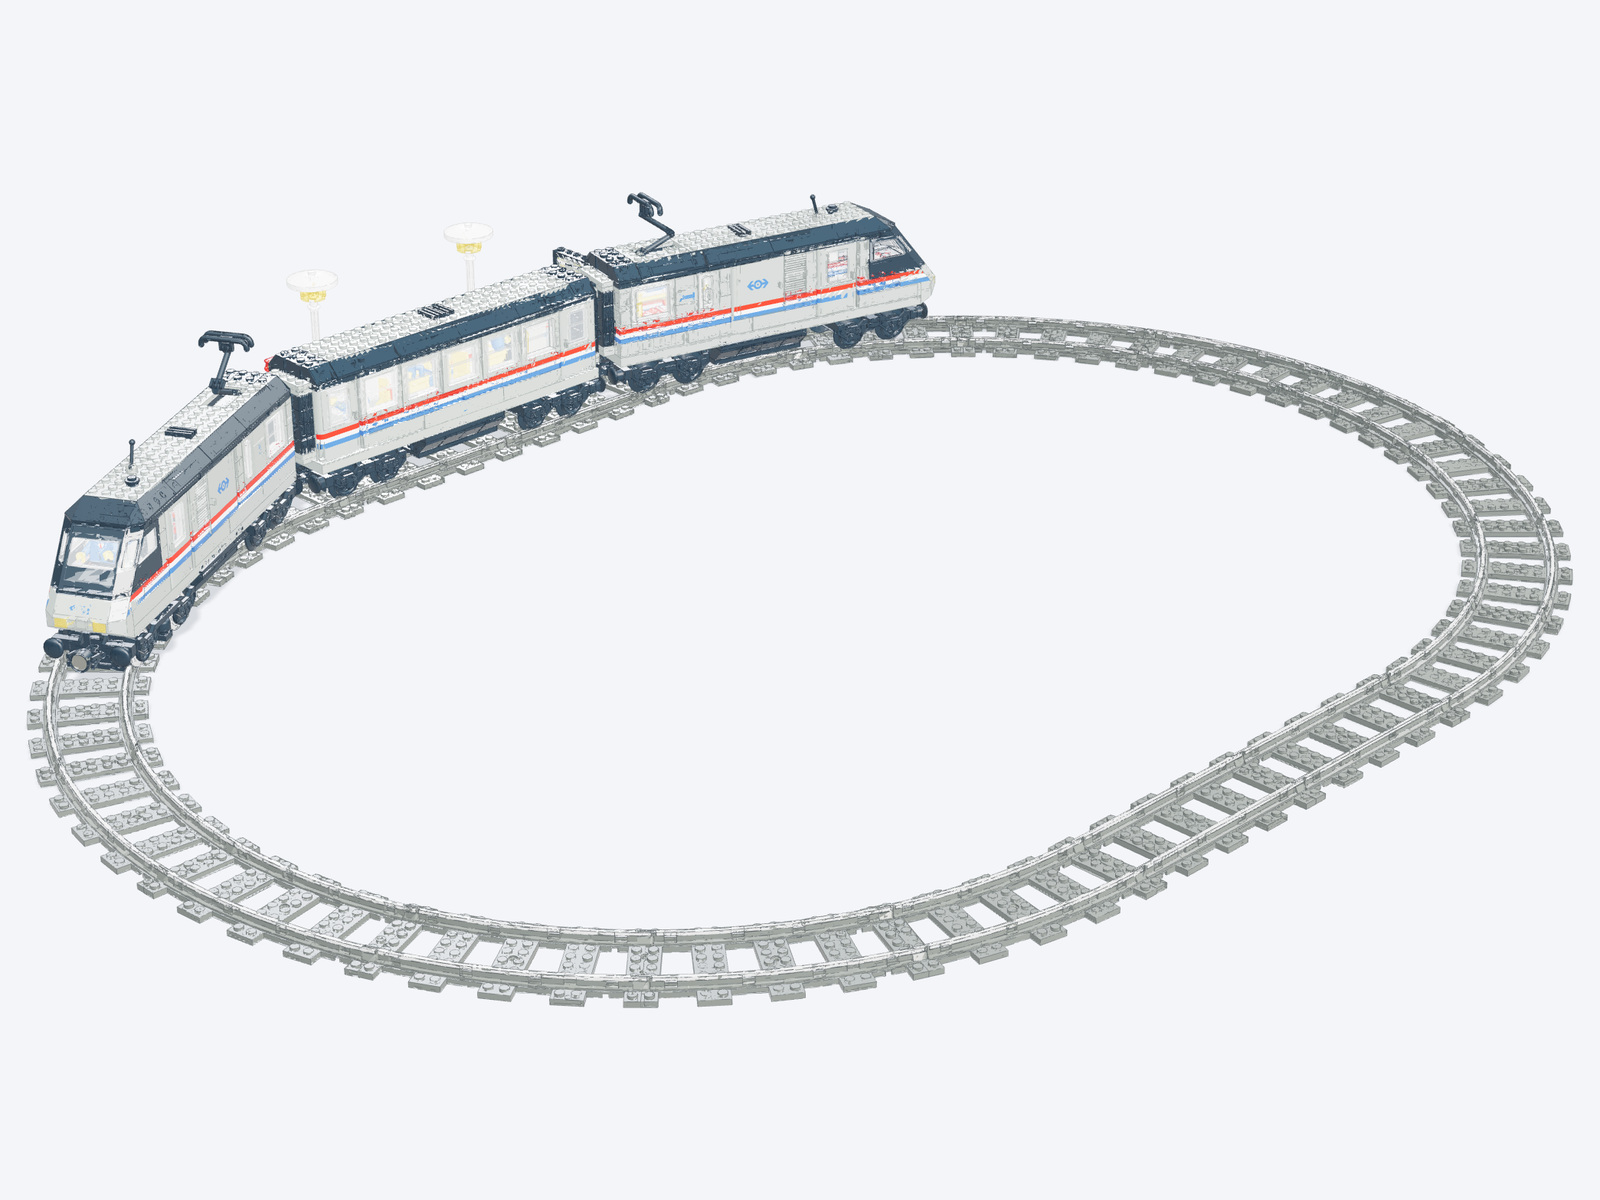
\includegraphics[width=.65\linewidth]{figures-v2/10001-iso.jpg}\end{center}
\paragraph{Attribution.}Zoltan Keri [kzoltan82]. CC BY 2.0.\par\url{https://library.ldraw.org/omr/sets/657}
\paragraph{Source SHA256.}\path{684a8032488dc2c5cb72a9ef32befb1399914eb32423e5b0cd91b6acfd3ab0e3}
\paragraph{Connector records.}stud: 2248; axle: 24; hinge: 96; fixed: 24; ball: 0
\paragraph{Public input lock.}\path{99cb64d39956d2ba1af371943780e3539e60539786c0938ebd1f8292099d11a0}
\paragraph{Status.}Source preservation does not certify stability. Reference outputs below are internal review material. Full model inputs are the versioned public JSON and numbered PNGs.
\begin{enumerate}
\item \textbf{ld2-10001-color-1}. Identify the original color of B0115; numbered isolation is allowed.
\par{\small color; visual; atomic; single-choice.\par\textit{Operands:} B0115 = brick\_000115\par\textit{Public evidence summary:} Numbered PNG: benchmark/ldraw-v2/inputs/views/ld2-10001-color-1.png; structured input = \{\}.\par\textit{Options:} A: Black; B: Trans Yellow; C: White; D: Trans Clear\par\textit{Reference output:} \{"choiceId": "A"\}\par\textit{Derivation:} source colorName by rendered B-label; source oracle only\par\textit{Equivalence:} exact declared response\par\textit{Review:} pending required human review.}
\item \textbf{ld2-10001-shape-match-1}. Ignoring color and pose, which numbered instance has the same LDraw part type as B0115?
\par{\small shape-match; visual; atomic; single-choice.\par\textit{Operands:} B0446 = brick\_000446, B0710 = brick\_000710, B0115 = brick\_000115, B0720 = brick\_000720, B0004 = brick\_000004\par\textit{Public evidence summary:} Numbered PNG: benchmark/ldraw-v2/inputs/views/ld2-10001-shape-match-1.png; structured input = \{\}.\par\textit{Options:} A: B0004; B: B0710; C: B0720; D: B0446\par\textit{Reference output:} \{"choiceId": "B"\}\par\textit{Derivation:} source partNumber equality across labeled candidates; source oracle only\par\textit{Equivalence:} same source partNumber; ignore color and pose; perceptual equivalence pending\par\textit{Review:} pending required human review.}
\item \textbf{ld2-10001-distance-1}. Using the supplied geometry bounding-box centers, which candidate is nearest to B0115?
\par{\small distance; source-data; atomic; single-choice.\par\textit{Operands:} B0115 = brick\_000115, B0272 = brick\_000272, B0050 = brick\_000050, B0720 = brick\_000720\par\textit{Public evidence summary:} \{"coordinateFrame": "Viewer world, millimeters, Euclidean distance", "centers": \{"B0115": [-74.436799, 20.8, 3.551199], "B0720": [343.856, 20.8, 30.516], "B0050": [-39.756, 13.2228, -92], "B0272": [-109.031199, 68.8, 0.431199]\}\}\par\textit{Options:} A: B0272; B: B0720; C: B0050\par\textit{Reference output:} \{"choiceId": "A"\}\par\textit{Derivation:} Euclidean norm from public rounded centers\par\textit{Equivalence:} exact declared response\par\textit{Review:} machine checks passed; no human certification.}
\item \textbf{ld2-10001-color-2}. Identify the original color of B0159; numbered isolation is allowed.
\par{\small color; visual; atomic; single-choice.\par\textit{Operands:} B0159 = brick\_000159\par\textit{Public evidence summary:} Numbered PNG: benchmark/ldraw-v2/inputs/views/ld2-10001-color-2.png; structured input = \{\}.\par\textit{Options:} A: White; B: Light Grey; C: Black; D: Brown\par\textit{Reference output:} \{"choiceId": "B"\}\par\textit{Derivation:} source colorName by rendered B-label; source oracle only\par\textit{Equivalence:} exact declared response\par\textit{Review:} pending required human review.}
\item \textbf{ld2-10001-shape-match-2}. Ignoring color and pose, which numbered instance has the same LDraw part type as B0159?
\par{\small shape-match; visual; atomic; single-choice.\par\textit{Operands:} B0192 = brick\_000192, B0794 = brick\_000794, B0165 = brick\_000165, B0163 = brick\_000163, B0159 = brick\_000159\par\textit{Public evidence summary:} Numbered PNG: benchmark/ldraw-v2/inputs/views/ld2-10001-shape-match-2.png; structured input = \{\}.\par\textit{Options:} A: B0192; B: B0794; C: B0165; D: B0163\par\textit{Reference output:} \{"choiceId": "D"\}\par\textit{Derivation:} source partNumber equality across labeled candidates; source oracle only\par\textit{Equivalence:} same source partNumber; ignore color and pose; perceptual equivalence pending\par\textit{Review:} pending required human review.}
\item \textbf{ld2-10001-distance-2}. Using the supplied geometry bounding-box centers, which candidate is nearest to B0159?
\par{\small distance; source-data; atomic; single-choice.\par\textit{Operands:} B0350 = brick\_000350, B0018 = brick\_000018, B0159 = brick\_000159, B0637 = brick\_000637\par\textit{Public evidence summary:} \{"coordinateFrame": "Viewer world, millimeters, Euclidean distance", "centers": \{"B0159": [-157.527199, 40, 28.431199], "B0350": [-140.599199, 88, 41.751199], "B0637": [370.82, 59.2, 41.768], "B0018": [-178.751951, 1.6, 570.031873]\}\}\par\textit{Options:} A: B0637; B: B0018; C: B0350\par\textit{Reference output:} \{"choiceId": "C"\}\par\textit{Derivation:} Euclidean norm from public rounded centers\par\textit{Equivalence:} exact declared response\par\textit{Review:} machine checks passed; no human certification.}
\item \textbf{ld2-10001-color-3}. Identify the original color of B0739; numbered isolation is allowed.
\par{\small color; visual; atomic; single-choice.\par\textit{Operands:} B0739 = brick\_000739\par\textit{Public evidence summary:} Numbered PNG: benchmark/ldraw-v2/inputs/views/ld2-10001-color-3.png; structured input = \{\}.\par\textit{Options:} A: Light Grey; B: Trans Yellow; C: Black; D: White\par\textit{Reference output:} \{"choiceId": "C"\}\par\textit{Derivation:} source colorName by rendered B-label; source oracle only\par\textit{Equivalence:} exact declared response\par\textit{Review:} pending required human review.}
\item \textbf{ld2-10001-shape-match-3}. Ignoring color and pose, which numbered instance has the same LDraw part type as B0739?
\par{\small shape-match; visual; atomic; single-choice.\par\textit{Operands:} B0739 = brick\_000739, B0712 = brick\_000712, B0776 = brick\_000776, B0546 = brick\_000546, B0023 = brick\_000023\par\textit{Public evidence summary:} Numbered PNG: benchmark/ldraw-v2/inputs/views/ld2-10001-shape-match-3.png; structured input = \{\}.\par\textit{Options:} A: B0546; B: B0712; C: B0776; D: B0023\par\textit{Reference output:} \{"choiceId": "B"\}\par\textit{Derivation:} source partNumber equality across labeled candidates; source oracle only\par\textit{Equivalence:} same source partNumber; ignore color and pose; perceptual equivalence pending\par\textit{Review:} pending required human review.}
\item \textbf{ld2-10001-distance-3}. Using the supplied geometry bounding-box centers, which candidate is nearest to B0739?
\par{\small distance; source-data; atomic; single-choice.\par\textit{Operands:} B0816 = brick\_000816, B0474 = brick\_000474, B0739 = brick\_000739, B0770 = brick\_000770\par\textit{Public evidence summary:} \{"coordinateFrame": "Viewer world, millimeters, Euclidean distance", "centers": \{"B0739": [275.744, 23.2, -21.2716], "B0816": [316.144, 59.2, -10.808], "B0474": [64, 40, -20], "B0770": [274.873286, 99.670801, -5.26347]\}\}\par\textit{Options:} A: B0816; B: B0770; C: B0474\par\textit{Reference output:} \{"choiceId": "A"\}\par\textit{Derivation:} Euclidean norm from public rounded centers\par\textit{Equivalence:} exact declared response\par\textit{Review:} machine checks passed; no human certification.}
\item \textbf{ld2-10001-color-4}. Identify the original color of B0826; numbered isolation is allowed.
\par{\small color; visual; atomic; single-choice.\par\textit{Operands:} B0826 = brick\_000826\par\textit{Public evidence summary:} Numbered PNG: benchmark/ldraw-v2/inputs/views/ld2-10001-color-4.png; structured input = \{\}.\par\textit{Options:} A: Trans Clear; B: Black; C: White; D: Brown\par\textit{Reference output:} \{"choiceId": "B"\}\par\textit{Derivation:} source colorName by rendered B-label; source oracle only\par\textit{Equivalence:} exact declared response\par\textit{Review:} pending required human review.}
\item \textbf{ld2-10001-shape-match-4}. Ignoring color and pose, which numbered instance has the same LDraw part type as B0826?
\par{\small shape-match; visual; atomic; single-choice.\par\textit{Operands:} B0826 = brick\_000826, B0079 = brick\_000079, B0121 = brick\_000121, B0581 = brick\_000581, B0137 = brick\_000137\par\textit{Public evidence summary:} Numbered PNG: benchmark/ldraw-v2/inputs/views/ld2-10001-shape-match-4.png; structured input = \{\}.\par\textit{Options:} A: B0137; B: B0079; C: B0121; D: B0581\par\textit{Reference output:} \{"choiceId": "C"\}\par\textit{Derivation:} source partNumber equality across labeled candidates; source oracle only\par\textit{Equivalence:} same source partNumber; ignore color and pose; perceptual equivalence pending\par\textit{Review:} pending required human review.}
\item \textbf{ld2-10001-distance-4}. Using the supplied geometry bounding-box centers, which candidate is nearest to B0826?
\par{\small distance; source-data; atomic; single-choice.\par\textit{Operands:} B0826 = brick\_000826, B0373 = brick\_000373, B0666 = brick\_000666, B0599 = brick\_000599\par\textit{Public evidence summary:} \{"coordinateFrame": "Viewer world, millimeters, Euclidean distance", "centers": \{"B0826": [230.90065, 19.05, -16.2808], "B0373": [208, 56, 0], "B0666": [369.2836, 78.4, -1.4436], "B0599": [254.82, 40, 11.724]\}\}\par\textit{Options:} A: B0373; B: B0666; C: B0599\par\textit{Reference output:} \{"choiceId": "C"\}\par\textit{Derivation:} Euclidean norm from public rounded centers\par\textit{Equivalence:} exact declared response\par\textit{Review:} pending required human review.}
\item \textbf{ld2-10001-interface-1}. Classify the supplied connector record for B0476 and B0477. This does not certify load capacity.
\par{\small interface; connector-graph; metacognitive; single-choice.\par\textit{Operands:} B0477 = brick\_000477, B0476 = brick\_000476\par\textit{Public evidence summary:} \{"connectorRecord": \{"family": "axle", "aConnector": 0, "bConnector": 0\}, "scope": "Upstream connector tolerances and inset mesh intersections; unknown parts remain explicit, separate scene objects are not glued together; no load/force validation."\}\par\textit{Options:} A: hinge; B: ball; C: fixed; D: stud; E: axle\par\textit{Reference output:} \{"choiceId": "E"\}\par\textit{Derivation:} public connectorRecord.family equality\par\textit{Equivalence:} exact declared response\par\textit{Review:} machine checks passed; no human certification.}
\item \textbf{ld2-10001-interface-2}. Classify the supplied connector record for B0101 and B0103. This does not certify load capacity.
\par{\small interface; connector-graph; metacognitive; single-choice.\par\textit{Operands:} B0101 = brick\_000101, B0103 = brick\_000103\par\textit{Public evidence summary:} \{"connectorRecord": \{"family": "fixed", "aConnector": 3, "bConnector": 1\}, "scope": "Upstream connector tolerances and inset mesh intersections; unknown parts remain explicit, separate scene objects are not glued together; no load/force validation."\}\par\textit{Options:} A: fixed; B: hinge; C: stud; D: axle; E: ball\par\textit{Reference output:} \{"choiceId": "A"\}\par\textit{Derivation:} public connectorRecord.family equality\par\textit{Equivalence:} exact declared response\par\textit{Review:} pending required human review.}
\item \textbf{ld2-10001-interface-3}. Classify the supplied connector record for B0840 and B0845. This does not certify load capacity.
\par{\small interface; connector-graph; metacognitive; single-choice.\par\textit{Operands:} B0845 = brick\_000845, B0840 = brick\_000840\par\textit{Public evidence summary:} \{"connectorRecord": \{"family": "hinge", "aConnector": 0, "bConnector": 6\}, "scope": "Upstream connector tolerances and inset mesh intersections; unknown parts remain explicit, separate scene objects are not glued together; no load/force validation."\}\par\textit{Options:} A: stud; B: hinge; C: fixed; D: ball; E: axle\par\textit{Reference output:} \{"choiceId": "B"\}\par\textit{Derivation:} public connectorRecord.family equality\par\textit{Equivalence:} exact declared response\par\textit{Review:} pending required human review.}
\item \textbf{ld2-10001-interface-4}. Classify the supplied connector record for B0592 and B0787. This does not certify load capacity.
\par{\small interface; connector-graph; metacognitive; single-choice.\par\textit{Operands:} B0592 = brick\_000592, B0787 = brick\_000787\par\textit{Public evidence summary:} \{"connectorRecord": \{"family": "stud", "aConnector": 225, "bConnector": 7\}, "scope": "Upstream connector tolerances and inset mesh intersections; unknown parts remain explicit, separate scene objects are not glued together; no load/force validation."\}\par\textit{Options:} A: stud; B: fixed; C: hinge; D: ball; E: axle\par\textit{Reference output:} \{"choiceId": "A"\}\par\textit{Derivation:} public connectorRecord.family equality\par\textit{Equivalence:} exact declared response\par\textit{Review:} pending required human review.}
\item \textbf{ld2-10001-neighbors-1}. Select every candidate directly adjacent to B0058 in the supplied connector graph.
\par{\small neighbors; connector-graph; metacognitive; multiple-choice.\par\textit{Operands:} B0484 = brick\_000484, B0053 = brick\_000053, B0052 = brick\_000052, B0058 = brick\_000058, B0076 = brick\_000076, B0653 = brick\_000653\par\textit{Public evidence summary:} 3 unique undirected pairs\par\textit{Options:} A: B0052; B: B0653; C: B0076; D: B0053; E: B0484\par\textit{Reference output:} \{"choiceIds": ["A", "C", "D"]\}\par\textit{Derivation:} public incident edge endpoint set\par\textit{Equivalence:} unordered exact set; duplicate IDs invalid\par\textit{Review:} pending required human review.}
\item \textbf{ld2-10001-graph-removal-1}. Delete B0058 and its incident edges from this local graph. How many connected components remain? Do not infer physical extractability.
\par{\small graph-removal; connector-graph; graph-internal; integer.\par\textit{Operands:} B0058 = brick\_000058, B0053 = brick\_000053, B0484 = brick\_000484, B0052 = brick\_000052, B0076 = brick\_000076, B0653 = brick\_000653\par\textit{Public evidence summary:} 3 unique undirected pairs; 6 nodes\par\textit{Reference output:} \{"value": 5\}\par\textit{Derivation:} union-find component count after public target deletion\par\textit{Equivalence:} exact declared response\par\textit{Review:} pending required human review.}
\item \textbf{ld2-10001-neighbors-2}. Select every candidate directly adjacent to B0734 in the supplied connector graph.
\par{\small neighbors; connector-graph; metacognitive; multiple-choice.\par\textit{Operands:} B0233 = brick\_000233, B0733 = brick\_000733, B0729 = brick\_000729, B0013 = brick\_000013, B0734 = brick\_000734, B0731 = brick\_000731\par\textit{Public evidence summary:} 3 unique undirected pairs\par\textit{Options:} A: B0013; B: B0733; C: B0729; D: B0233; E: B0731\par\textit{Reference output:} \{"choiceIds": ["B", "C", "E"]\}\par\textit{Derivation:} public incident edge endpoint set\par\textit{Equivalence:} unordered exact set; duplicate IDs invalid\par\textit{Review:} pending required human review.}
\item \textbf{ld2-10001-graph-removal-2}. Delete B0734 and its incident edges from this local graph. How many connected components remain? Do not infer physical extractability.
\par{\small graph-removal; connector-graph; graph-internal; integer.\par\textit{Operands:} B0731 = brick\_000731, B0733 = brick\_000733, B0013 = brick\_000013, B0734 = brick\_000734, B0233 = brick\_000233, B0729 = brick\_000729\par\textit{Public evidence summary:} 3 unique undirected pairs; 6 nodes\par\textit{Reference output:} \{"value": 5\}\par\textit{Derivation:} union-find component count after public target deletion\par\textit{Equivalence:} exact declared response\par\textit{Review:} pending required human review.}
\item \textbf{ld2-10001-neighbors-3}. Select every candidate directly adjacent to B0828 in the supplied connector graph.
\par{\small neighbors; connector-graph; metacognitive; multiple-choice.\par\textit{Operands:} B0836 = brick\_000836, B0677 = brick\_000677, B0833 = brick\_000833, B0834 = brick\_000834, B0549 = brick\_000549, B0828 = brick\_000828\par\textit{Public evidence summary:} 3 unique undirected pairs\par\textit{Options:} A: B0836; B: B0833; C: B0834; D: B0677; E: B0549\par\textit{Reference output:} \{"choiceIds": ["A", "B", "C"]\}\par\textit{Derivation:} public incident edge endpoint set\par\textit{Equivalence:} unordered exact set; duplicate IDs invalid\par\textit{Review:} pending required human review.}
\item \textbf{ld2-10001-graph-removal-3}. Delete B0828 and its incident edges from this local graph. How many connected components remain? Do not infer physical extractability.
\par{\small graph-removal; connector-graph; graph-internal; integer.\par\textit{Operands:} B0677 = brick\_000677, B0834 = brick\_000834, B0549 = brick\_000549, B0833 = brick\_000833, B0836 = brick\_000836, B0828 = brick\_000828\par\textit{Public evidence summary:} 3 unique undirected pairs; 6 nodes\par\textit{Reference output:} \{"value": 5\}\par\textit{Derivation:} union-find component count after public target deletion\par\textit{Equivalence:} exact declared response\par\textit{Review:} pending required human review.}
\item \textbf{ld2-10001-neighbors-4}. Select every candidate directly adjacent to B0447 in the supplied connector graph.
\par{\small neighbors; connector-graph; metacognitive; multiple-choice.\par\textit{Operands:} B0593 = brick\_000593, B0447 = brick\_000447, B0442 = brick\_000442, B0444 = brick\_000444, B0012 = brick\_000012, B0445 = brick\_000445, B0439 = brick\_000439, B0440 = brick\_000440\par\textit{Public evidence summary:} 5 unique undirected pairs\par\textit{Options:} A: B0445; B: B0444; C: B0442; D: B0593; E: B0012; F: B0439; G: B0440\par\textit{Reference output:} \{"choiceIds": ["A", "B", "C", "F", "G"]\}\par\textit{Derivation:} public incident edge endpoint set\par\textit{Equivalence:} unordered exact set; duplicate IDs invalid\par\textit{Review:} pending required human review.}
\item \textbf{ld2-10001-graph-removal-4}. Delete B0447 and its incident edges from this local graph. How many connected components remain? Do not infer physical extractability.
\par{\small graph-removal; connector-graph; graph-internal; integer.\par\textit{Operands:} B0440 = brick\_000440, B0445 = brick\_000445, B0439 = brick\_000439, B0444 = brick\_000444, B0442 = brick\_000442, B0447 = brick\_000447, B0012 = brick\_000012, B0593 = brick\_000593\par\textit{Public evidence summary:} 5 unique undirected pairs; 8 nodes\par\textit{Reference output:} \{"value": 7\}\par\textit{Derivation:} union-find component count after public target deletion\par\textit{Equivalence:} exact declared response\par\textit{Review:} pending required human review.}
\item \textbf{ld2-10001-coverage-1}. Which numbered instance lacks a connector definition in the coverage record, so this audit cannot establish that it is floating?
\par{\small coverage; source-data; metacognitive; single-choice.\par\textit{Operands:} B0739 = brick\_000739, B0159 = brick\_000159, B0115 = brick\_000115, B0092 = brick\_000092\par\textit{Public evidence summary:} \{"coverage": [\{"label": "B0739", "supported": true\}, \{"label": "B0115", "supported": true\}, \{"label": "B0159", "supported": true\}, \{"label": "B0092", "supported": false\}]\}\par\textit{Options:} A: B0739; B: B0159; C: B0092; D: B0115\par\textit{Reference output:} \{"choiceId": "C"\}\par\textit{Derivation:} public supported=false record\par\textit{Equivalence:} exact declared response\par\textit{Review:} pending required human review.}
\item \textbf{ld2-10001-evidence-limit-1}. Only source geometry, connector matching and mesh intersection audits are available. Without mass, friction, material or dynamic tests, is gravitational stability established?
\par{\small evidence-limit; source-data; metacognitive; single-choice.\par\textit{Operands:} none\par\textit{Public evidence summary:} \{"available": ["Original CAD", "Connector inference", "Inset-mesh intersection candidates"]\}\par\textit{Options:} A: Established; B: Not established by this evidence\par\textit{Reference output:} \{"choiceId": "B"\}\par\textit{Derivation:} fixed epistemic control label\par\textit{Equivalence:} exact declared response\par\textit{Review:} machine checks passed; no human certification.}
\item \textbf{ld2-10001-source-step-1}. At which expanded author step does B0037 first appear in the supplied source-step table? Source order is not a collision-free assembly proof.
\par{\small source-step; source-data; procedural; single-choice.\par\textit{Operands:} B0001 = brick\_000001, B0037 = brick\_000037\par\textit{Public evidence summary:} 2 supplied author-step records; exact table in public JSON\par\textit{Options:} A: 4; B: 3; C: 2; D: 1\par\textit{Reference output:} \{"choiceId": "A"\}\par\textit{Derivation:} minimum public step index containing target\par\textit{Equivalence:} exact declared response\par\textit{Review:} pending required human review.}
\item \textbf{ld2-10001-source-step-2}. At which expanded author step does B0079 first appear in the supplied source-step table? Source order is not a collision-free assembly proof.
\par{\small source-step; source-data; procedural; single-choice.\par\textit{Operands:} B0079 = brick\_000079, B0001 = brick\_000001\par\textit{Public evidence summary:} 2 supplied author-step records; exact table in public JSON\par\textit{Options:} A: 25; B: 7; C: 26; D: 13\par\textit{Reference output:} \{"choiceId": "B"\}\par\textit{Derivation:} minimum public step index containing target\par\textit{Equivalence:} exact declared response\par\textit{Review:} pending required human review.}
\item \textbf{ld2-10001-source-step-3}. At which expanded author step does B0052 first appear in the supplied source-step table? Source order is not a collision-free assembly proof.
\par{\small source-step; source-data; procedural; single-choice.\par\textit{Operands:} B0052 = brick\_000052, B0001 = brick\_000001\par\textit{Public evidence summary:} 2 supplied author-step records; exact table in public JSON\par\textit{Options:} A: 1; B: 5; C: 4; D: 3\par\textit{Reference output:} \{"choiceId": "B"\}\par\textit{Derivation:} minimum public step index containing target\par\textit{Equivalence:} exact declared response\par\textit{Review:} pending required human review.}
\item \textbf{ld2-10001-source-step-4}. At which expanded author step does B0104 first appear in the supplied source-step table? Source order is not a collision-free assembly proof.
\par{\small source-step; source-data; procedural; single-choice.\par\textit{Operands:} B0104 = brick\_000104, B0001 = brick\_000001\par\textit{Public evidence summary:} 2 supplied author-step records; exact table in public JSON\par\textit{Options:} A: 8; B: 9; C: 18; D: 6\par\textit{Reference output:} \{"choiceId": "B"\}\par\textit{Derivation:} minimum public step index containing target\par\textit{Equivalence:} exact declared response\par\textit{Review:} pending required human review.}
\item \textbf{ld2-10001-source-sequence-1}. Reveal the supplied source-step window in author order. Actions change visibility only, without simulating insertion trajectories.
\par{\small source-sequence; scene-edit; procedural; actions.\par\textit{Operands:} B0021 = brick\_000021, B0046 = brick\_000046, B0059 = brick\_000059, B0073 = brick\_000073, B0066 = brick\_000066, B0078 = brick\_000078, B0038 = brick\_000038, B0003 = brick\_000003, B0029 = brick\_000029, B0005 = brick\_000005, B0024 = brick\_000024, B0012 = brick\_000012, B0036 = brick\_000036, B0014 = brick\_000014, B0034 = brick\_000034, B0065 = brick\_000065, B0067 = brick\_000067, B0020 = brick\_000020, B0060 = brick\_000060, B0007 = brick\_000007, B0011 = brick\_000011, B0040 = brick\_000040, B0070 = brick\_000070, B0010 = brick\_000010, B0042 = brick\_000042, B0015 = brick\_000015, B0023 = brick\_000023, B0043 = brick\_000043, B0049 = brick\_000049, B0008 = brick\_000008, B0063 = brick\_000063, B0045 = brick\_000045, B0033 = brick\_000033, B0002 = brick\_000002, B0064 = brick\_000064, B0051 = brick\_000051, B0035 = brick\_000035, B0047 = brick\_000047, B0072 = brick\_000072, B0048 = brick\_000048, B0006 = brick\_000006, B0053 = brick\_000053, B0018 = brick\_000018, B0077 = brick\_000077, B0013 = brick\_000013, B0016 = brick\_000016, B0030 = brick\_000030, B0069 = brick\_000069, B0041 = brick\_000041, B0052 = brick\_000052, B0056 = brick\_000056, B0058 = brick\_000058, B0031 = brick\_000031, B0032 = brick\_000032, B0004 = brick\_000004, B0074 = brick\_000074, B0050 = brick\_000050, B0037 = brick\_000037, B0009 = brick\_000009, B0068 = brick\_000068, B0022 = brick\_000022, B0062 = brick\_000062, B0057 = brick\_000057, B0061 = brick\_000061, B0019 = brick\_000019, B0001 = brick\_000001, B0017 = brick\_000017, B0075 = brick\_000075, B0076 = brick\_000076, B0039 = brick\_000039, B0025 = brick\_000025, B0028 = brick\_000028, B0044 = brick\_000044, B0071 = brick\_000071, B0026 = brick\_000026, B0054 = brick\_000054, B0027 = brick\_000027, B0055 = brick\_000055\par\textit{Public evidence summary:} 6 public actions; budget 6; \{"initialFacts": ["start"], "goalFacts": ["done-6"], "absentFacts": []\}\par\textit{Reference output:} \{"actionIds": ["step-1", "step-2", "step-3", "step-4", "step-5", "step-6"]\}\par\textit{Derivation:} public precondition solver\par\textit{Equivalence:} any legal sequence reaching all goals within budget; display-only semantics\par\textit{Review:} pending required human review.}
\item \textbf{ld2-10001-restore-instance-1}. The display copy hides B0115. Restore only that numbered instance, preserving all other instances and source poses.
\par{\small restore-instance; scene-edit; procedural; actions.\par\textit{Operands:} B0001 = brick\_000001, B0115 = brick\_000115\par\textit{Public evidence summary:} 2 public actions; budget 1; \{"initialFacts": ["missing-brick\_000115", "present-brick\_000001"], "goalFacts": ["present-brick\_000115", "present-brick\_000001"], "absentFacts": ["missing-brick\_000115"]\}\par\textit{Reference output:} \{"actionIds": ["restore-B0115"]\}\par\textit{Derivation:} public precondition solver\par\textit{Equivalence:} any legal sequence reaching all goals within budget; display-only semantics\par\textit{Review:} pending required human review.}
\item \textbf{ld2-10001-restore-instance-2}. The display copy hides B0159. Restore only that numbered instance, preserving all other instances and source poses.
\par{\small restore-instance; scene-edit; procedural; actions.\par\textit{Operands:} B0159 = brick\_000159, B0001 = brick\_000001\par\textit{Public evidence summary:} 2 public actions; budget 1; \{"initialFacts": ["missing-brick\_000159", "present-brick\_000001"], "goalFacts": ["present-brick\_000159", "present-brick\_000001"], "absentFacts": ["missing-brick\_000159"]\}\par\textit{Reference output:} \{"actionIds": ["restore-B0159"]\}\par\textit{Derivation:} public precondition solver\par\textit{Equivalence:} any legal sequence reaching all goals within budget; display-only semantics\par\textit{Review:} pending required human review.}
\item \textbf{ld2-10001-restore-instance-3}. The display copy hides B0739. Restore only that numbered instance, preserving all other instances and source poses.
\par{\small restore-instance; scene-edit; procedural; actions.\par\textit{Operands:} B0001 = brick\_000001, B0739 = brick\_000739\par\textit{Public evidence summary:} 2 public actions; budget 1; \{"initialFacts": ["missing-brick\_000739", "present-brick\_000001"], "goalFacts": ["present-brick\_000739", "present-brick\_000001"], "absentFacts": ["missing-brick\_000739"]\}\par\textit{Reference output:} \{"actionIds": ["restore-B0739"]\}\par\textit{Derivation:} public precondition solver\par\textit{Equivalence:} any legal sequence reaching all goals within budget; display-only semantics\par\textit{Review:} pending required human review.}
\end{enumerate}
\clearpage\section{10269: Harley-Davidson Fat Boy}
1029 source instances; 34 tasks; D4 size band. 225 type strings; 16 color codes; 12 unsupported instances; 40 intersection candidates. 340 expanded author steps. Independent reparse: passed.
\begin{center}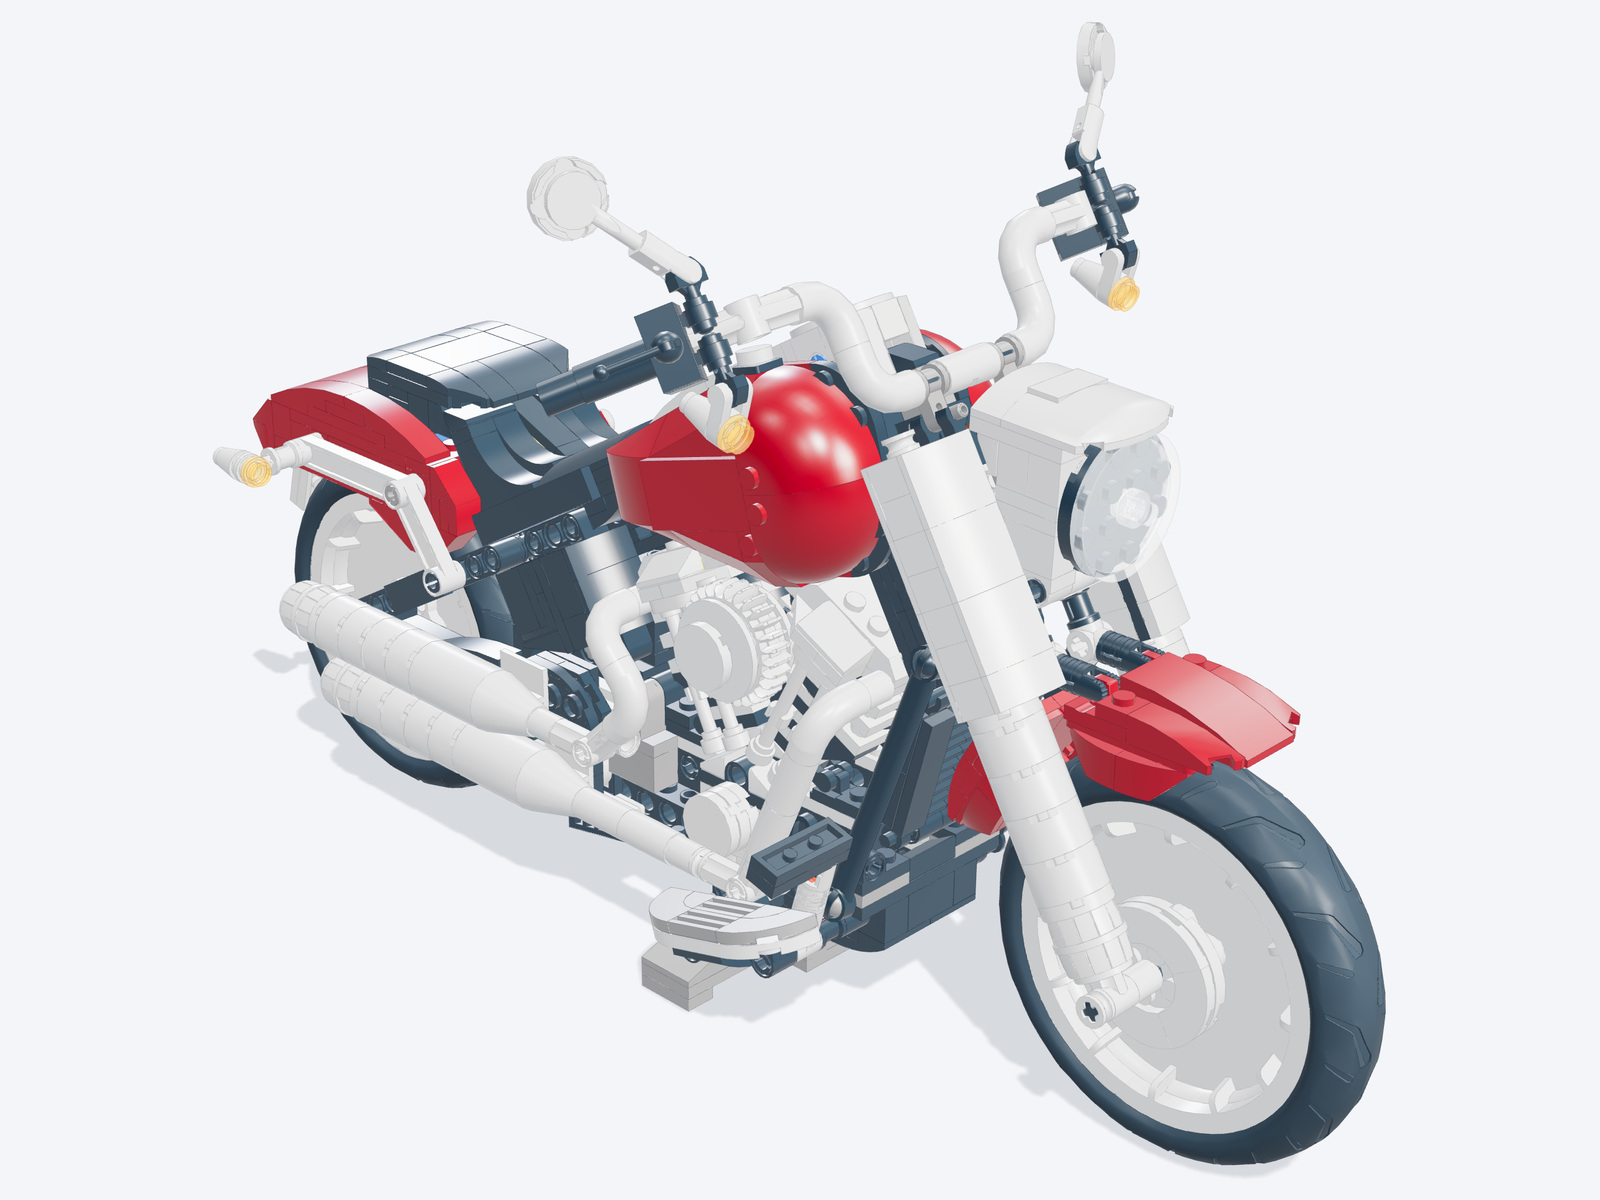
\includegraphics[width=.65\linewidth]{figures-v2/omr-10269-iso.jpg}\end{center}
\paragraph{Attribution.}Orion Pobursky [OrionP]. CC BY 2.0.\par\url{https://library.ldraw.org/library/omr/10269-1.mpd}
\paragraph{Source SHA256.}\path{777f57f34cc8f4bddcee0ff94d81bfefd615b7ad4e92ab668cedb66d4b29f476}
\paragraph{Connector records.}stud: 1638; axle: 437; hinge: 50; fixed: 0; ball: 4
\paragraph{Public input lock.}\path{25ba21e39ed4d4933199c3b30ecf244b1b5edefb976b26b72dd1dc3c76bf89ff}
\paragraph{Status.}Source preservation does not certify stability. Reference outputs below are internal review material. Full model inputs are the versioned public JSON and numbered PNGs.
\begin{enumerate}
\item \textbf{ld2-omr-10269-color-1}. Identify the original color of B0802; numbered isolation is allowed.
\par{\small color; visual; atomic; single-choice.\par\textit{Operands:} B0802 = brick\_000802\par\textit{Public evidence summary:} Numbered PNG: benchmark/ldraw-v2/inputs/views/ld2-omr-10269-color-1.png; structured input = \{\}.\par\textit{Options:} A: Reddish Brown; B: Rubber Black; C: Light Bluish Grey; D: Sand Blue\par\textit{Reference output:} \{"choiceId": "C"\}\par\textit{Derivation:} source colorName by rendered B-label; source oracle only\par\textit{Equivalence:} exact declared response\par\textit{Review:} pending required human review.}
\item \textbf{ld2-omr-10269-shape-match-1}. Ignoring color and pose, which numbered instance has the same LDraw part type as B0802?
\par{\small shape-match; visual; atomic; single-choice.\par\textit{Operands:} B0136 = brick\_000136, B0636 = brick\_000636, B0979 = brick\_000979, B0056 = brick\_000056, B0802 = brick\_000802\par\textit{Public evidence summary:} Numbered PNG: benchmark/ldraw-v2/inputs/views/ld2-omr-10269-shape-match-1.png; structured input = \{\}.\par\textit{Options:} A: B0056; B: B0979; C: B0636; D: B0136\par\textit{Reference output:} \{"choiceId": "D"\}\par\textit{Derivation:} source partNumber equality across labeled candidates; source oracle only\par\textit{Equivalence:} same source partNumber; ignore color and pose; perceptual equivalence pending\par\textit{Review:} pending required human review.}
\item \textbf{ld2-omr-10269-distance-1}. Using the supplied geometry bounding-box centers, which candidate is nearest to B0802?
\par{\small distance; source-data; atomic; single-choice.\par\textit{Operands:} B0407 = brick\_000407, B0796 = brick\_000796, B0950 = brick\_000950, B0802 = brick\_000802\par\textit{Public evidence summary:} \{"coordinateFrame": "Viewer world, millimeters, Euclidean distance", "centers": \{"B0802": [32.8, 64.264, -107.36], "B0407": [24, 58.380604, -65.432031], "B0950": [12, 149.6982, 72.237453], "B0796": [-48, 29.1214, 10.6146]\}\}\par\textit{Options:} A: B0796; B: B0950; C: B0407\par\textit{Reference output:} \{"choiceId": "C"\}\par\textit{Derivation:} Euclidean norm from public rounded centers\par\textit{Equivalence:} exact declared response\par\textit{Review:} machine checks passed; no human certification.}
\item \textbf{ld2-omr-10269-color-2}. Identify the original color of B0626; numbered isolation is allowed.
\par{\small color; visual; atomic; single-choice.\par\textit{Operands:} B0626 = brick\_000626\par\textit{Public evidence summary:} Numbered PNG: benchmark/ldraw-v2/inputs/views/ld2-omr-10269-color-2.png; structured input = \{\}.\par\textit{Options:} A: Yellow; B: Trans Red; C: Dark Bluish Grey; D: Dark Red\par\textit{Reference output:} \{"choiceId": "A"\}\par\textit{Derivation:} source colorName by rendered B-label; source oracle only\par\textit{Equivalence:} exact declared response\par\textit{Review:} pending required human review.}
\item \textbf{ld2-omr-10269-shape-match-2}. Ignoring color and pose, which numbered instance has the same LDraw part type as B0626?
\par{\small shape-match; visual; atomic; single-choice.\par\textit{Operands:} B0970 = brick\_000970, B0626 = brick\_000626, B0359 = brick\_000359, B0405 = brick\_000405, B0474 = brick\_000474\par\textit{Public evidence summary:} Numbered PNG: benchmark/ldraw-v2/inputs/views/ld2-omr-10269-shape-match-2.png; structured input = \{\}.\par\textit{Options:} A: B0359; B: B0405; C: B0970; D: B0474\par\textit{Reference output:} \{"choiceId": "D"\}\par\textit{Derivation:} source partNumber equality across labeled candidates; source oracle only\par\textit{Equivalence:} same source partNumber; ignore color and pose; perceptual equivalence pending\par\textit{Review:} pending required human review.}
\item \textbf{ld2-omr-10269-distance-2}. Using the supplied geometry bounding-box centers, which candidate is nearest to B0626?
\par{\small distance; source-data; atomic; single-choice.\par\textit{Operands:} B0492 = brick\_000492, B0911 = brick\_000911, B0626 = brick\_000626, B0388 = brick\_000388\par\textit{Public evidence summary:} \{"coordinateFrame": "Viewer world, millimeters, Euclidean distance", "centers": \{"B0626": [0, 133.4356, -8.7248], "B0388": [24, 26.5669, -98.571706], "B0911": [12, 44.1108, 118.6532], "B0492": [20, 95.7316, -99.5424]\}\}\par\textit{Options:} A: B0911; B: B0492; C: B0388\par\textit{Reference output:} \{"choiceId": "B"\}\par\textit{Derivation:} Euclidean norm from public rounded centers\par\textit{Equivalence:} exact declared response\par\textit{Review:} machine checks passed; no human certification.}
\item \textbf{ld2-omr-10269-color-3}. Identify the original color of B0487; numbered isolation is allowed.
\par{\small color; visual; atomic; single-choice.\par\textit{Operands:} B0487 = brick\_000487\par\textit{Public evidence summary:} Numbered PNG: benchmark/ldraw-v2/inputs/views/ld2-omr-10269-color-3.png; structured input = \{\}.\par\textit{Options:} A: Dark Red; B: Black; C: Light Bluish Grey; D: Blue\par\textit{Reference output:} \{"choiceId": "A"\}\par\textit{Derivation:} source colorName by rendered B-label; source oracle only\par\textit{Equivalence:} exact declared response\par\textit{Review:} pending required human review.}
\item \textbf{ld2-omr-10269-shape-match-3}. Ignoring color and pose, which numbered instance has the same LDraw part type as B0487?
\par{\small shape-match; visual; atomic; single-choice.\par\textit{Operands:} B0255 = brick\_000255, B0586 = brick\_000586, B0483 = brick\_000483, B0487 = brick\_000487, B0608 = brick\_000608\par\textit{Public evidence summary:} Numbered PNG: benchmark/ldraw-v2/inputs/views/ld2-omr-10269-shape-match-3.png; structured input = \{\}.\par\textit{Options:} A: B0586; B: B0608; C: B0255; D: B0483\par\textit{Reference output:} \{"choiceId": "D"\}\par\textit{Derivation:} source partNumber equality across labeled candidates; source oracle only\par\textit{Equivalence:} same source partNumber; ignore color and pose; perceptual equivalence pending\par\textit{Review:} pending required human review.}
\item \textbf{ld2-omr-10269-distance-3}. Using the supplied geometry bounding-box centers, which candidate is nearest to B0487?
\par{\small distance; source-data; atomic; single-choice.\par\textit{Operands:} B0242 = brick\_000242, B0487 = brick\_000487, B0865 = brick\_000865, B0317 = brick\_000317\par\textit{Public evidence summary:} \{"coordinateFrame": "Viewer world, millimeters, Euclidean distance", "centers": \{"B0487": [4, 108.5316, -129.1424], "B0317": [8, 95.208418, 52.719016], "B0242": [0, 98.6624, 21.9632], "B0865": [-24, 141.1188, 61.0124]\}\}\par\textit{Options:} A: B0242; B: B0865; C: B0317\par\textit{Reference output:} \{"choiceId": "A"\}\par\textit{Derivation:} Euclidean norm from public rounded centers\par\textit{Equivalence:} exact declared response\par\textit{Review:} machine checks passed; no human certification.}
\item \textbf{ld2-omr-10269-color-4}. Identify the original color of B0033; numbered isolation is allowed.
\par{\small color; visual; atomic; single-choice.\par\textit{Operands:} B0033 = brick\_000033\par\textit{Public evidence summary:} Numbered PNG: benchmark/ldraw-v2/inputs/views/ld2-omr-10269-color-4.png; structured input = \{\}.\par\textit{Options:} A: Dark Bluish Grey; B: Red; C: Light Bluish Grey; D: Trans Orange\par\textit{Reference output:} \{"choiceId": "C"\}\par\textit{Derivation:} source colorName by rendered B-label; source oracle only\par\textit{Equivalence:} exact declared response\par\textit{Review:} pending required human review.}
\item \textbf{ld2-omr-10269-shape-match-4}. Ignoring color and pose, which numbered instance has the same LDraw part type as B0033?
\par{\small shape-match; visual; atomic; single-choice.\par\textit{Operands:} B0468 = brick\_000468, B0033 = brick\_000033, B0685 = brick\_000685, B0314 = brick\_000314, B0990 = brick\_000990\par\textit{Public evidence summary:} Numbered PNG: benchmark/ldraw-v2/inputs/views/ld2-omr-10269-shape-match-4.png; structured input = \{\}.\par\textit{Options:} A: B0685; B: B0468; C: B0314; D: B0990\par\textit{Reference output:} \{"choiceId": "B"\}\par\textit{Derivation:} source partNumber equality across labeled candidates; source oracle only\par\textit{Equivalence:} same source partNumber; ignore color and pose; perceptual equivalence pending\par\textit{Review:} pending required human review.}
\item \textbf{ld2-omr-10269-distance-4}. Using the supplied geometry bounding-box centers, which candidate is nearest to B0033?
\par{\small distance; source-data; atomic; single-choice.\par\textit{Operands:} B0003 = brick\_000003, B0147 = brick\_000147, B0374 = brick\_000374, B0033 = brick\_000033\par\textit{Public evidence summary:} \{"coordinateFrame": "Viewer world, millimeters, Euclidean distance", "centers": \{"B0033": [20, 28, 12], "B0003": [12, 21.6, -60], "B0374": [-8, 120.2692, 26.2124], "B0147": [-12, 34.4, 28]\}\}\par\textit{Options:} A: B0003; B: B0374; C: B0147\par\textit{Reference output:} \{"choiceId": "C"\}\par\textit{Derivation:} Euclidean norm from public rounded centers\par\textit{Equivalence:} exact declared response\par\textit{Review:} machine checks passed; no human certification.}
\item \textbf{ld2-omr-10269-interface-1}. Classify the supplied connector record for B0090 and B0091. This does not certify load capacity.
\par{\small interface; connector-graph; metacognitive; single-choice.\par\textit{Operands:} B0091 = brick\_000091, B0090 = brick\_000090\par\textit{Public evidence summary:} \{"connectorRecord": \{"family": "axle", "aConnector": 22, "bConnector": 1\}, "scope": "Upstream connector tolerances and inset mesh intersections; unknown parts remain explicit, separate scene objects are not glued together; no load/force validation."\}\par\textit{Options:} A: axle; B: fixed; C: stud; D: ball; E: hinge\par\textit{Reference output:} \{"choiceId": "A"\}\par\textit{Derivation:} public connectorRecord.family equality\par\textit{Equivalence:} exact declared response\par\textit{Review:} machine checks passed; no human certification.}
\item \textbf{ld2-omr-10269-interface-2}. Classify the supplied connector record for B0045 and B0433. This does not certify load capacity.
\par{\small interface; connector-graph; metacognitive; single-choice.\par\textit{Operands:} B0433 = brick\_000433, B0045 = brick\_000045\par\textit{Public evidence summary:} \{"connectorRecord": \{"family": "ball", "aConnector": 3, "bConnector": 0\}, "scope": "Upstream connector tolerances and inset mesh intersections; unknown parts remain explicit, separate scene objects are not glued together; no load/force validation."\}\par\textit{Options:} A: ball; B: fixed; C: axle; D: stud; E: hinge\par\textit{Reference output:} \{"choiceId": "A"\}\par\textit{Derivation:} public connectorRecord.family equality\par\textit{Equivalence:} exact declared response\par\textit{Review:} machine checks passed; no human certification.}
\item \textbf{ld2-omr-10269-interface-3}. Classify the supplied connector record for B0384 and B0383. This does not certify load capacity.
\par{\small interface; connector-graph; metacognitive; single-choice.\par\textit{Operands:} B0383 = brick\_000383, B0384 = brick\_000384\par\textit{Public evidence summary:} \{"connectorRecord": \{"family": "hinge", "aConnector": 0, "bConnector": 1\}, "scope": "Upstream connector tolerances and inset mesh intersections; unknown parts remain explicit, separate scene objects are not glued together; no load/force validation."\}\par\textit{Options:} A: fixed; B: hinge; C: ball; D: stud; E: axle\par\textit{Reference output:} \{"choiceId": "B"\}\par\textit{Derivation:} public connectorRecord.family equality\par\textit{Equivalence:} exact declared response\par\textit{Review:} pending required human review.}
\item \textbf{ld2-omr-10269-interface-4}. Classify the supplied connector record for B0454 and B0456. This does not certify load capacity.
\par{\small interface; connector-graph; metacognitive; single-choice.\par\textit{Operands:} B0456 = brick\_000456, B0454 = brick\_000454\par\textit{Public evidence summary:} \{"connectorRecord": \{"family": "stud", "aConnector": 10, "bConnector": 2\}, "scope": "Upstream connector tolerances and inset mesh intersections; unknown parts remain explicit, separate scene objects are not glued together; no load/force validation."\}\par\textit{Options:} A: fixed; B: axle; C: hinge; D: ball; E: stud\par\textit{Reference output:} \{"choiceId": "E"\}\par\textit{Derivation:} public connectorRecord.family equality\par\textit{Equivalence:} exact declared response\par\textit{Review:} pending required human review.}
\item \textbf{ld2-omr-10269-neighbors-1}. Select every candidate directly adjacent to B0282 in the supplied connector graph.
\par{\small neighbors; connector-graph; metacognitive; multiple-choice.\par\textit{Operands:} B0282 = brick\_000282, B0283 = brick\_000283, B0265 = brick\_000265, B0413 = brick\_000413, B0284 = brick\_000284, B0618 = brick\_000618, B0280 = brick\_000280\par\textit{Public evidence summary:} 4 unique undirected pairs\par\textit{Options:} A: B0280; B: B0283; C: B0265; D: B0618; E: B0284; F: B0413\par\textit{Reference output:} \{"choiceIds": ["A", "B", "C", "E"]\}\par\textit{Derivation:} public incident edge endpoint set\par\textit{Equivalence:} unordered exact set; duplicate IDs invalid\par\textit{Review:} pending required human review.}
\item \textbf{ld2-omr-10269-graph-removal-1}. Delete B0282 and its incident edges from this local graph. How many connected components remain? Do not infer physical extractability.
\par{\small graph-removal; connector-graph; graph-internal; integer.\par\textit{Operands:} B0413 = brick\_000413, B0283 = brick\_000283, B0284 = brick\_000284, B0265 = brick\_000265, B0280 = brick\_000280, B0618 = brick\_000618, B0282 = brick\_000282\par\textit{Public evidence summary:} 4 unique undirected pairs; 7 nodes\par\textit{Reference output:} \{"value": 6\}\par\textit{Derivation:} union-find component count after public target deletion\par\textit{Equivalence:} exact declared response\par\textit{Review:} pending required human review.}
\item \textbf{ld2-omr-10269-neighbors-2}. Select every candidate directly adjacent to B0764 in the supplied connector graph.
\par{\small neighbors; connector-graph; metacognitive; multiple-choice.\par\textit{Operands:} B0766 = brick\_000766, B0762 = brick\_000762, B0053 = brick\_000053, B0763 = brick\_000763, B0422 = brick\_000422, B0764 = brick\_000764, B0765 = brick\_000765\par\textit{Public evidence summary:} 5 unique undirected pairs\par\textit{Options:} A: B0762; B: B0765; C: B0422; D: B0763; E: B0766; F: B0053\par\textit{Reference output:} \{"choiceIds": ["A", "B", "D", "E"]\}\par\textit{Derivation:} public incident edge endpoint set\par\textit{Equivalence:} unordered exact set; duplicate IDs invalid\par\textit{Review:} machine checks passed; no human certification.}
\item \textbf{ld2-omr-10269-graph-removal-2}. Delete B0764 and its incident edges from this local graph. How many connected components remain? Do not infer physical extractability.
\par{\small graph-removal; connector-graph; graph-internal; integer.\par\textit{Operands:} B0053 = brick\_000053, B0766 = brick\_000766, B0764 = brick\_000764, B0422 = brick\_000422, B0765 = brick\_000765, B0763 = brick\_000763, B0762 = brick\_000762\par\textit{Public evidence summary:} 5 unique undirected pairs; 7 nodes\par\textit{Reference output:} \{"value": 5\}\par\textit{Derivation:} union-find component count after public target deletion\par\textit{Equivalence:} exact declared response\par\textit{Review:} machine checks passed; no human certification.}
\item \textbf{ld2-omr-10269-neighbors-3}. Select every candidate directly adjacent to B0973 in the supplied connector graph.
\par{\small neighbors; connector-graph; metacognitive; multiple-choice.\par\textit{Operands:} B0836 = brick\_000836, B0972 = brick\_000972, B0624 = brick\_000624, B0973 = brick\_000973, B0975 = brick\_000975\par\textit{Public evidence summary:} 2 unique undirected pairs\par\textit{Options:} A: B0975; B: B0836; C: B0972; D: B0624\par\textit{Reference output:} \{"choiceIds": ["A", "C"]\}\par\textit{Derivation:} public incident edge endpoint set\par\textit{Equivalence:} unordered exact set; duplicate IDs invalid\par\textit{Review:} machine checks passed; no human certification.}
\item \textbf{ld2-omr-10269-graph-removal-3}. Delete B0973 and its incident edges from this local graph. How many connected components remain? Do not infer physical extractability.
\par{\small graph-removal; connector-graph; graph-internal; integer.\par\textit{Operands:} B0975 = brick\_000975, B0836 = brick\_000836, B0973 = brick\_000973, B0624 = brick\_000624, B0972 = brick\_000972\par\textit{Public evidence summary:} 2 unique undirected pairs; 5 nodes\par\textit{Reference output:} \{"value": 4\}\par\textit{Derivation:} union-find component count after public target deletion\par\textit{Equivalence:} exact declared response\par\textit{Review:} machine checks passed; no human certification.}
\item \textbf{ld2-omr-10269-neighbors-4}. Select every candidate directly adjacent to B0127 in the supplied connector graph.
\par{\small neighbors; connector-graph; metacognitive; multiple-choice.\par\textit{Operands:} B0128 = brick\_000128, B0126 = brick\_000126, B0127 = brick\_000127, B0129 = brick\_000129, B0537 = brick\_000537, B0130 = brick\_000130, B0681 = brick\_000681\par\textit{Public evidence summary:} 4 unique undirected pairs\par\textit{Options:} A: B0129; B: B0126; C: B0681; D: B0130; E: B0128; F: B0537\par\textit{Reference output:} \{"choiceIds": ["A", "B", "D", "E"]\}\par\textit{Derivation:} public incident edge endpoint set\par\textit{Equivalence:} unordered exact set; duplicate IDs invalid\par\textit{Review:} pending required human review.}
\item \textbf{ld2-omr-10269-graph-removal-4}. Delete B0127 and its incident edges from this local graph. How many connected components remain? Do not infer physical extractability.
\par{\small graph-removal; connector-graph; graph-internal; integer.\par\textit{Operands:} B0128 = brick\_000128, B0130 = brick\_000130, B0126 = brick\_000126, B0129 = brick\_000129, B0127 = brick\_000127, B0681 = brick\_000681, B0537 = brick\_000537\par\textit{Public evidence summary:} 4 unique undirected pairs; 7 nodes\par\textit{Reference output:} \{"value": 6\}\par\textit{Derivation:} union-find component count after public target deletion\par\textit{Equivalence:} exact declared response\par\textit{Review:} pending required human review.}
\item \textbf{ld2-omr-10269-coverage-1}. Which numbered instance lacks a connector definition in the coverage record, so this audit cannot establish that it is floating?
\par{\small coverage; source-data; metacognitive; single-choice.\par\textit{Operands:} B0487 = brick\_000487, B0802 = brick\_000802, B0626 = brick\_000626, B0256 = brick\_000256\par\textit{Public evidence summary:} \{"coverage": [\{"label": "B0802", "supported": true\}, \{"label": "B0626", "supported": true\}, \{"label": "B0487", "supported": true\}, \{"label": "B0256", "supported": false\}]\}\par\textit{Options:} A: B0802; B: B0487; C: B0256; D: B0626\par\textit{Reference output:} \{"choiceId": "C"\}\par\textit{Derivation:} public supported=false record\par\textit{Equivalence:} exact declared response\par\textit{Review:} pending required human review.}
\item \textbf{ld2-omr-10269-evidence-limit-1}. Only source geometry, connector matching and mesh intersection audits are available. Without mass, friction, material or dynamic tests, is gravitational stability established?
\par{\small evidence-limit; source-data; metacognitive; single-choice.\par\textit{Operands:} none\par\textit{Public evidence summary:} \{"available": ["Original CAD", "Connector inference", "Inset-mesh intersection candidates"]\}\par\textit{Options:} A: Established; B: Not established by this evidence\par\textit{Reference output:} \{"choiceId": "B"\}\par\textit{Derivation:} fixed epistemic control label\par\textit{Equivalence:} exact declared response\par\textit{Review:} machine checks passed; no human certification.}
\item \textbf{ld2-omr-10269-source-step-1}. At which expanded author step does B0533 first appear in the supplied source-step table? Source order is not a collision-free assembly proof.
\par{\small source-step; source-data; procedural; single-choice.\par\textit{Operands:} B0001 = brick\_000001, B0533 = brick\_000533\par\textit{Public evidence summary:} 2 supplied author-step records; exact table in public JSON\par\textit{Options:} A: 324; B: 335; C: 269; D: 152\par\textit{Reference output:} \{"choiceId": "D"\}\par\textit{Derivation:} minimum public step index containing target\par\textit{Equivalence:} exact declared response\par\textit{Review:} machine checks passed; no human certification.}
\item \textbf{ld2-omr-10269-source-step-2}. At which expanded author step does B0037 first appear in the supplied source-step table? Source order is not a collision-free assembly proof.
\par{\small source-step; source-data; procedural; single-choice.\par\textit{Operands:} B0037 = brick\_000037, B0001 = brick\_000001\par\textit{Public evidence summary:} 2 supplied author-step records; exact table in public JSON\par\textit{Options:} A: 328; B: 10; C: 2; D: 131\par\textit{Reference output:} \{"choiceId": "B"\}\par\textit{Derivation:} minimum public step index containing target\par\textit{Equivalence:} exact declared response\par\textit{Review:} machine checks passed; no human certification.}
\item \textbf{ld2-omr-10269-source-step-3}. At which expanded author step does B0667 first appear in the supplied source-step table? Source order is not a collision-free assembly proof.
\par{\small source-step; source-data; procedural; single-choice.\par\textit{Operands:} B0667 = brick\_000667, B0001 = brick\_000001\par\textit{Public evidence summary:} 2 supplied author-step records; exact table in public JSON\par\textit{Options:} A: 182; B: 67; C: 204; D: 29\par\textit{Reference output:} \{"choiceId": "C"\}\par\textit{Derivation:} minimum public step index containing target\par\textit{Equivalence:} exact declared response\par\textit{Review:} machine checks passed; no human certification.}
\item \textbf{ld2-omr-10269-source-step-4}. At which expanded author step does B0767 first appear in the supplied source-step table? Source order is not a collision-free assembly proof.
\par{\small source-step; source-data; procedural; single-choice.\par\textit{Operands:} B0001 = brick\_000001, B0767 = brick\_000767\par\textit{Public evidence summary:} 2 supplied author-step records; exact table in public JSON\par\textit{Options:} A: 253; B: 318; C: 243; D: 133\par\textit{Reference output:} \{"choiceId": "C"\}\par\textit{Derivation:} minimum public step index containing target\par\textit{Equivalence:} exact declared response\par\textit{Review:} machine checks passed; no human certification.}
\item \textbf{ld2-omr-10269-source-sequence-1}. Reveal the supplied source-step window in author order. Actions change visibility only, without simulating insertion trajectories.
\par{\small source-sequence; scene-edit; procedural; actions.\par\textit{Operands:} B0016 = brick\_000016, B0003 = brick\_000003, B0006 = brick\_000006, B0017 = brick\_000017, B0009 = brick\_000009, B0001 = brick\_000001, B0011 = brick\_000011, B0004 = brick\_000004, B0005 = brick\_000005, B0002 = brick\_000002, B0013 = brick\_000013, B0012 = brick\_000012, B0015 = brick\_000015, B0022 = brick\_000022, B0020 = brick\_000020, B0018 = brick\_000018, B0008 = brick\_000008, B0007 = brick\_000007, B0019 = brick\_000019, B0021 = brick\_000021, B0010 = brick\_000010, B0023 = brick\_000023, B0014 = brick\_000014\par\textit{Public evidence summary:} 6 public actions; budget 6; \{"initialFacts": ["start"], "goalFacts": ["done-6"], "absentFacts": []\}\par\textit{Reference output:} \{"actionIds": ["step-1", "step-2", "step-3", "step-4", "step-5", "step-6"]\}\par\textit{Derivation:} public precondition solver\par\textit{Equivalence:} any legal sequence reaching all goals within budget; display-only semantics\par\textit{Review:} machine checks passed; no human certification.}
\item \textbf{ld2-omr-10269-restore-instance-1}. The display copy hides B0802. Restore only that numbered instance, preserving all other instances and source poses.
\par{\small restore-instance; scene-edit; procedural; actions.\par\textit{Operands:} B0001 = brick\_000001, B0802 = brick\_000802\par\textit{Public evidence summary:} 2 public actions; budget 1; \{"initialFacts": ["missing-brick\_000802", "present-brick\_000001"], "goalFacts": ["present-brick\_000802", "present-brick\_000001"], "absentFacts": ["missing-brick\_000802"]\}\par\textit{Reference output:} \{"actionIds": ["restore-B0802"]\}\par\textit{Derivation:} public precondition solver\par\textit{Equivalence:} any legal sequence reaching all goals within budget; display-only semantics\par\textit{Review:} machine checks passed; no human certification.}
\item \textbf{ld2-omr-10269-restore-instance-2}. The display copy hides B0626. Restore only that numbered instance, preserving all other instances and source poses.
\par{\small restore-instance; scene-edit; procedural; actions.\par\textit{Operands:} B0626 = brick\_000626, B0001 = brick\_000001\par\textit{Public evidence summary:} 2 public actions; budget 1; \{"initialFacts": ["missing-brick\_000626", "present-brick\_000001"], "goalFacts": ["present-brick\_000626", "present-brick\_000001"], "absentFacts": ["missing-brick\_000626"]\}\par\textit{Reference output:} \{"actionIds": ["restore-B0626"]\}\par\textit{Derivation:} public precondition solver\par\textit{Equivalence:} any legal sequence reaching all goals within budget; display-only semantics\par\textit{Review:} machine checks passed; no human certification.}
\item \textbf{ld2-omr-10269-restore-instance-3}. The display copy hides B0487. Restore only that numbered instance, preserving all other instances and source poses.
\par{\small restore-instance; scene-edit; procedural; actions.\par\textit{Operands:} B0001 = brick\_000001, B0487 = brick\_000487\par\textit{Public evidence summary:} 2 public actions; budget 1; \{"initialFacts": ["missing-brick\_000487", "present-brick\_000001"], "goalFacts": ["present-brick\_000487", "present-brick\_000001"], "absentFacts": ["missing-brick\_000487"]\}\par\textit{Reference output:} \{"actionIds": ["restore-B0487"]\}\par\textit{Derivation:} public precondition solver\par\textit{Equivalence:} any legal sequence reaching all goals within budget; display-only semantics\par\textit{Review:} machine checks passed; no human certification.}
\end{enumerate}
\clearpage\section{10242: MINI Cooper}
1086 source instances; 34 tasks; D4 size band. 136 type strings; 22 color codes; 10 unsupported instances; 17 intersection candidates. 233 expanded author steps. Independent reparse: passed.
\begin{center}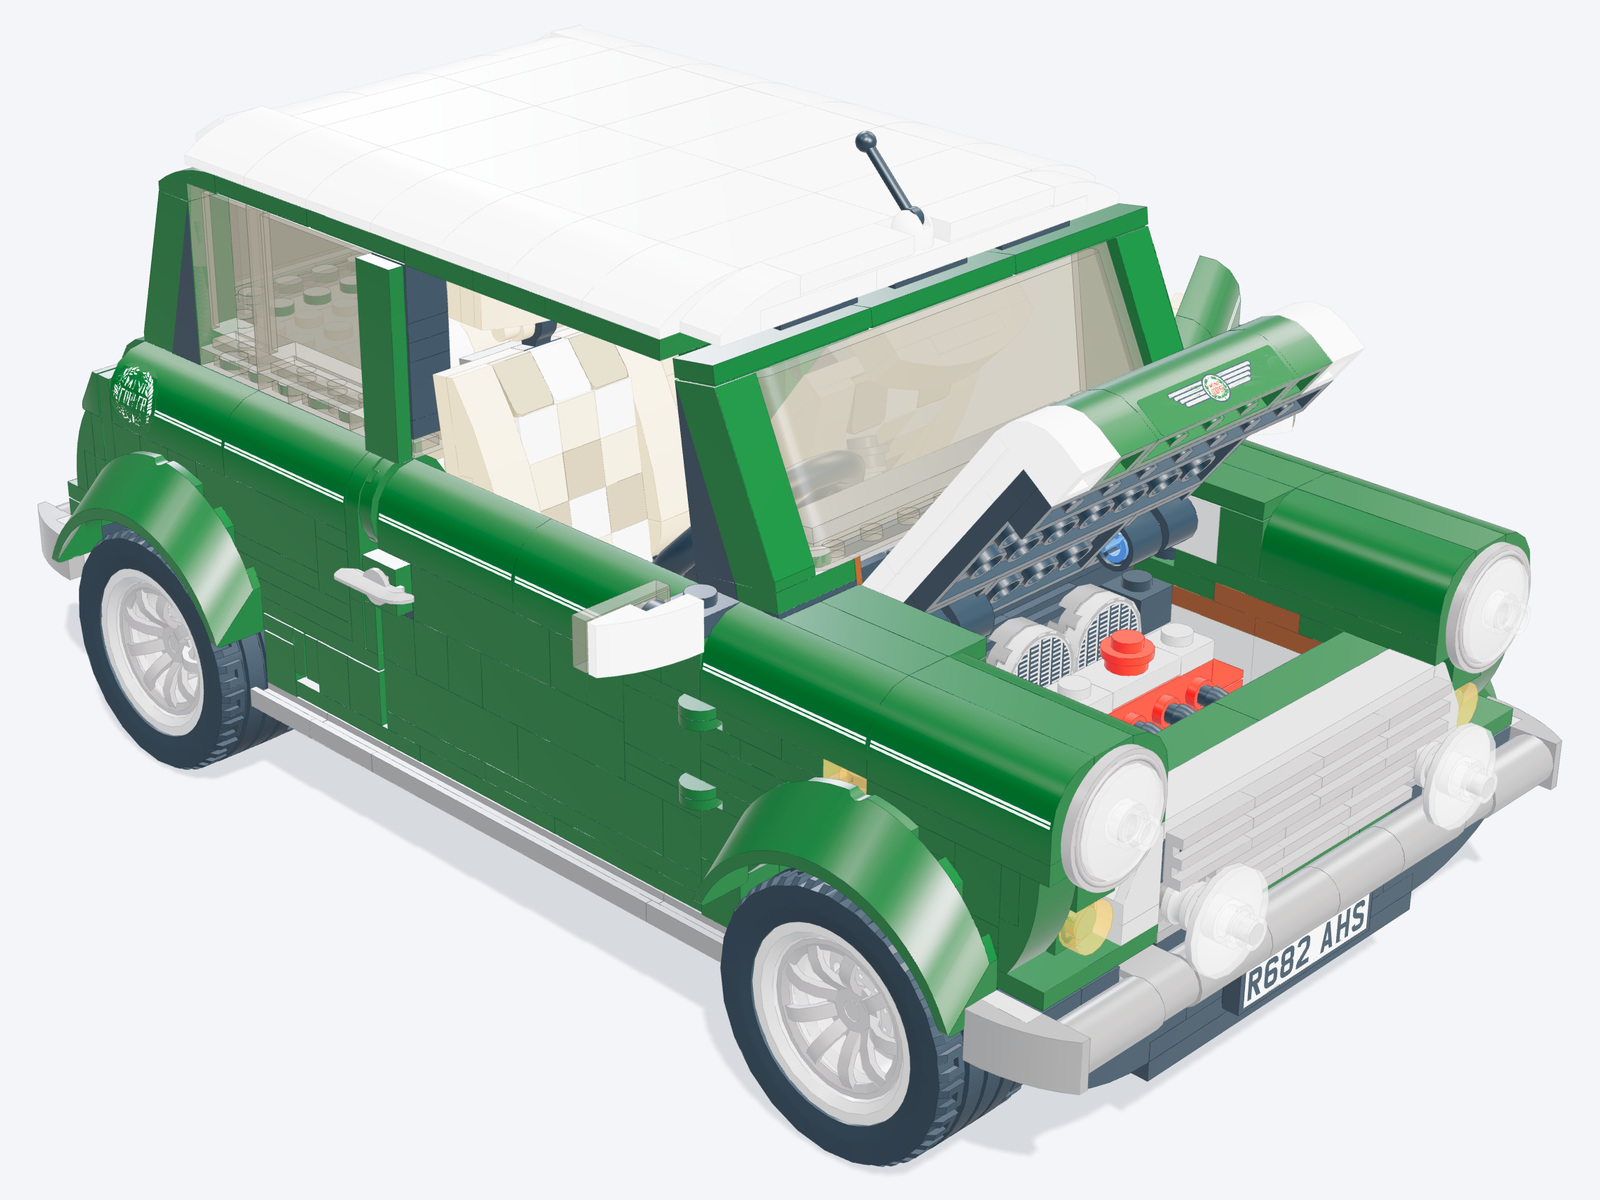
\includegraphics[width=.65\linewidth]{figures-v2/omr-10242-iso.jpg}\end{center}
\paragraph{Attribution.}Magnus Forsberg [MagFors]. CC BY 2.0.\par\url{https://library.ldraw.org/library/omr/10242-1.mpd}
\paragraph{Source SHA256.}\path{d79fd06503b145cc5ff3c5bcfe71a1c402910dee78424f54077faba9cf402b74}
\paragraph{Connector records.}stud: 2293; axle: 161; hinge: 7; fixed: 20; ball: 0
\paragraph{Public input lock.}\path{9e9a4464b790765d8611cd98f178ffe0da91c11d977e386c0c91f3be7dd0f599}
\paragraph{Status.}Source preservation does not certify stability. Reference outputs below are internal review material. Full model inputs are the versioned public JSON and numbered PNGs.
\begin{enumerate}
\item \textbf{ld2-omr-10242-color-1}. Identify the original color of B0591; numbered isolation is allowed.
\par{\small color; visual; atomic; single-choice.\par\textit{Operands:} B0591 = brick\_000591\par\textit{Public evidence summary:} Numbered PNG: benchmark/ldraw-v2/inputs/views/ld2-omr-10242-color-1.png; structured input = \{\}.\par\textit{Options:} A: Reddish Brown; B: White; C: Trans Light Blue; D: Pearl Gold\par\textit{Reference output:} \{"choiceId": "A"\}\par\textit{Derivation:} source colorName by rendered B-label; source oracle only\par\textit{Equivalence:} exact declared response\par\textit{Review:} pending required human review.}
\item \textbf{ld2-omr-10242-shape-match-1}. Ignoring color and pose, which numbered instance has the same LDraw part type as B0591?
\par{\small shape-match; visual; atomic; single-choice.\par\textit{Operands:} B0591 = brick\_000591, B0304 = brick\_000304, B0281 = brick\_000281, B0512 = brick\_000512, B0073 = brick\_000073\par\textit{Public evidence summary:} Numbered PNG: benchmark/ldraw-v2/inputs/views/ld2-omr-10242-shape-match-1.png; structured input = \{\}.\par\textit{Options:} A: B0281; B: B0304; C: B0073; D: B0512\par\textit{Reference output:} \{"choiceId": "C"\}\par\textit{Derivation:} source partNumber equality across labeled candidates; source oracle only\par\textit{Equivalence:} same source partNumber; ignore color and pose; perceptual equivalence pending\par\textit{Review:} pending required human review.}
\item \textbf{ld2-omr-10242-distance-1}. Using the supplied geometry bounding-box centers, which candidate is nearest to B0591?
\par{\small distance; source-data; atomic; single-choice.\par\textit{Operands:} B0669 = brick\_000669, B0840 = brick\_000840, B0950 = brick\_000950, B0591 = brick\_000591\par\textit{Public evidence summary:} \{"coordinateFrame": "Viewer world, millimeters, Euclidean distance", "centers": \{"B0591": [44, 34.4, 64], "B0669": [-12, 20.726885, 90.813115], "B0950": [60.928, 31.2, 42.122316], "B0840": [8, 24.059068, -4.9024]\}\}\par\textit{Options:} A: B0669; B: B0840; C: B0950\par\textit{Reference output:} \{"choiceId": "C"\}\par\textit{Derivation:} Euclidean norm from public rounded centers\par\textit{Equivalence:} exact declared response\par\textit{Review:} pending required human review.}
\item \textbf{ld2-omr-10242-color-2}. Identify the original color of B0837; numbered isolation is allowed.
\par{\small color; visual; atomic; single-choice.\par\textit{Operands:} B0837 = brick\_000837\par\textit{Public evidence summary:} Numbered PNG: benchmark/ldraw-v2/inputs/views/ld2-omr-10242-color-2.png; structured input = \{\}.\par\textit{Options:} A: Trans Clear; B: Yellow; C: White; D: Tan\par\textit{Reference output:} \{"choiceId": "D"\}\par\textit{Derivation:} source colorName by rendered B-label; source oracle only\par\textit{Equivalence:} exact declared response\par\textit{Review:} pending required human review.}
\item \textbf{ld2-omr-10242-shape-match-2}. Ignoring color and pose, which numbered instance has the same LDraw part type as B0837?
\par{\small shape-match; visual; atomic; single-choice.\par\textit{Operands:} B0166 = brick\_000166, B0341 = brick\_000341, B0837 = brick\_000837, B0845 = brick\_000845, B0303 = brick\_000303\par\textit{Public evidence summary:} Numbered PNG: benchmark/ldraw-v2/inputs/views/ld2-omr-10242-shape-match-2.png; structured input = \{\}.\par\textit{Options:} A: B0166; B: B0303; C: B0845; D: B0341\par\textit{Reference output:} \{"choiceId": "B"\}\par\textit{Derivation:} source partNumber equality across labeled candidates; source oracle only\par\textit{Equivalence:} same source partNumber; ignore color and pose; perceptual equivalence pending\par\textit{Review:} pending required human review.}
\item \textbf{ld2-omr-10242-distance-2}. Using the supplied geometry bounding-box centers, which candidate is nearest to B0837?
\par{\small distance; source-data; atomic; single-choice.\par\textit{Operands:} B0103 = brick\_000103, B0465 = brick\_000465, B0837 = brick\_000837, B0511 = brick\_000511\par\textit{Public evidence summary:} \{"coordinateFrame": "Viewer world, millimeters, Euclidean distance", "centers": \{"B0837": [40, 31.6984, -0.1184], "B0465": [-36, 21.6, 44], "B0511": [0, 37.6, 38.4], "B0103": [0, 5.6, 116]\}\}\par\textit{Options:} A: B0103; B: B0465; C: B0511\par\textit{Reference output:} \{"choiceId": "C"\}\par\textit{Derivation:} Euclidean norm from public rounded centers\par\textit{Equivalence:} exact declared response\par\textit{Review:} pending required human review.}
\item \textbf{ld2-omr-10242-color-3}. Identify the original color of B0962; numbered isolation is allowed.
\par{\small color; visual; atomic; single-choice.\par\textit{Operands:} B0962 = brick\_000962\par\textit{Public evidence summary:} Numbered PNG: benchmark/ldraw-v2/inputs/views/ld2-omr-10242-color-3.png; structured input = \{\}.\par\textit{Options:} A: Bright Light Orange; B: Trans Brown; C: Medium Nougat; D: Black\par\textit{Reference output:} \{"choiceId": "D"\}\par\textit{Derivation:} source colorName by rendered B-label; source oracle only\par\textit{Equivalence:} exact declared response\par\textit{Review:} pending required human review.}
\item \textbf{ld2-omr-10242-shape-match-3}. Ignoring color and pose, which numbered instance has the same LDraw part type as B0962?
\par{\small shape-match; visual; atomic; single-choice.\par\textit{Operands:} B0969 = brick\_000969, B0962 = brick\_000962, B0654 = brick\_000654, B0610 = brick\_000610, B0111 = brick\_000111\par\textit{Public evidence summary:} Numbered PNG: benchmark/ldraw-v2/inputs/views/ld2-omr-10242-shape-match-3.png; structured input = \{\}.\par\textit{Options:} A: B0111; B: B0654; C: B0610; D: B0969\par\textit{Reference output:} \{"choiceId": "B"\}\par\textit{Derivation:} source partNumber equality across labeled candidates; source oracle only\par\textit{Equivalence:} same source partNumber; ignore color and pose; perceptual equivalence pending\par\textit{Review:} pending required human review.}
\item \textbf{ld2-omr-10242-distance-3}. Using the supplied geometry bounding-box centers, which candidate is nearest to B0962?
\par{\small distance; source-data; atomic; single-choice.\par\textit{Operands:} B0714 = brick\_000714, B0029 = brick\_000029, B0962 = brick\_000962, B0312 = brick\_000312\par\textit{Public evidence summary:} \{"coordinateFrame": "Viewer world, millimeters, Euclidean distance", "centers": \{"B0962": [58.7176, 44, 45.1072], "B0714": [36, 21.6, -60], "B0029": [24, -4, -40], "B0312": [-36, 24.8, -80]\}\}\par\textit{Options:} A: B0714; B: B0312; C: B0029\par\textit{Reference output:} \{"choiceId": "C"\}\par\textit{Derivation:} Euclidean norm from public rounded centers\par\textit{Equivalence:} exact declared response\par\textit{Review:} machine checks passed; no human certification.}
\item \textbf{ld2-omr-10242-color-4}. Identify the original color of B0975; numbered isolation is allowed.
\par{\small color; visual; atomic; single-choice.\par\textit{Operands:} B0975 = brick\_000975\par\textit{Public evidence summary:} Numbered PNG: benchmark/ldraw-v2/inputs/views/ld2-omr-10242-color-4.png; structured input = \{\}.\par\textit{Options:} A: Dark Green; B: Trans Brown; C: Medium Nougat; D: Yellow\par\textit{Reference output:} \{"choiceId": "A"\}\par\textit{Derivation:} source colorName by rendered B-label; source oracle only\par\textit{Equivalence:} exact declared response\par\textit{Review:} pending required human review.}
\item \textbf{ld2-omr-10242-shape-match-4}. Ignoring color and pose, which numbered instance has the same LDraw part type as B0975?
\par{\small shape-match; visual; atomic; single-choice.\par\textit{Operands:} B0485 = brick\_000485, B0180 = brick\_000180, B0975 = brick\_000975, B1004 = brick\_001004, B0657 = brick\_000657\par\textit{Public evidence summary:} Numbered PNG: benchmark/ldraw-v2/inputs/views/ld2-omr-10242-shape-match-4.png; structured input = \{\}.\par\textit{Options:} A: B0657; B: B0485; C: B1004; D: B0180\par\textit{Reference output:} \{"choiceId": "B"\}\par\textit{Derivation:} source partNumber equality across labeled candidates; source oracle only\par\textit{Equivalence:} same source partNumber; ignore color and pose; perceptual equivalence pending\par\textit{Review:} pending required human review.}
\item \textbf{ld2-omr-10242-distance-4}. Using the supplied geometry bounding-box centers, which candidate is nearest to B0975?
\par{\small distance; source-data; atomic; single-choice.\par\textit{Operands:} B0857 = brick\_000857, B0379 = brick\_000379, B0265 = brick\_000265, B0975 = brick\_000975\par\textit{Public evidence summary:} \{"coordinateFrame": "Viewer world, millimeters, Euclidean distance", "centers": \{"B0975": [-51.2, 28, 28], "B0857": [24, 59.534, 21.9088], "B0379": [-40, 37.6, -68], "B0265": [48, 5.6, -44]\}\}\par\textit{Options:} A: B0379; B: B0265; C: B0857\par\textit{Reference output:} \{"choiceId": "C"\}\par\textit{Derivation:} Euclidean norm from public rounded centers\par\textit{Equivalence:} exact declared response\par\textit{Review:} machine checks passed; no human certification.}
\item \textbf{ld2-omr-10242-interface-1}. Classify the supplied connector record for B0028 and B0032. This does not certify load capacity.
\par{\small interface; connector-graph; metacognitive; single-choice.\par\textit{Operands:} B0032 = brick\_000032, B0028 = brick\_000028\par\textit{Public evidence summary:} \{"connectorRecord": \{"family": "axle", "aConnector": 12, "bConnector": 0\}, "scope": "Upstream connector tolerances and inset mesh intersections; unknown parts remain explicit, separate scene objects are not glued together; no load/force validation."\}\par\textit{Options:} A: hinge; B: axle; C: ball; D: stud; E: fixed\par\textit{Reference output:} \{"choiceId": "B"\}\par\textit{Derivation:} public connectorRecord.family equality\par\textit{Equivalence:} exact declared response\par\textit{Review:} machine checks passed; no human certification.}
\item \textbf{ld2-omr-10242-interface-2}. Classify the supplied connector record for B0153 and B0154. This does not certify load capacity.
\par{\small interface; connector-graph; metacognitive; single-choice.\par\textit{Operands:} B0153 = brick\_000153, B0154 = brick\_000154\par\textit{Public evidence summary:} \{"connectorRecord": \{"family": "fixed", "aConnector": 1, "bConnector": 1\}, "scope": "Upstream connector tolerances and inset mesh intersections; unknown parts remain explicit, separate scene objects are not glued together; no load/force validation."\}\par\textit{Options:} A: axle; B: stud; C: fixed; D: hinge; E: ball\par\textit{Reference output:} \{"choiceId": "C"\}\par\textit{Derivation:} public connectorRecord.family equality\par\textit{Equivalence:} exact declared response\par\textit{Review:} machine checks passed; no human certification.}
\item \textbf{ld2-omr-10242-interface-3}. Classify the supplied connector record for B0578 and B0981. This does not certify load capacity.
\par{\small interface; connector-graph; metacognitive; single-choice.\par\textit{Operands:} B0578 = brick\_000578, B0981 = brick\_000981\par\textit{Public evidence summary:} \{"connectorRecord": \{"family": "hinge", "aConnector": 1, "bConnector": 2\}, "scope": "Upstream connector tolerances and inset mesh intersections; unknown parts remain explicit, separate scene objects are not glued together; no load/force validation."\}\par\textit{Options:} A: ball; B: fixed; C: hinge; D: axle; E: stud\par\textit{Reference output:} \{"choiceId": "C"\}\par\textit{Derivation:} public connectorRecord.family equality\par\textit{Equivalence:} exact declared response\par\textit{Review:} machine checks passed; no human certification.}
\item \textbf{ld2-omr-10242-interface-4}. Classify the supplied connector record for B1027 and B1034. This does not certify load capacity.
\par{\small interface; connector-graph; metacognitive; single-choice.\par\textit{Operands:} B1027 = brick\_001027, B1034 = brick\_001034\par\textit{Public evidence summary:} \{"connectorRecord": \{"family": "stud", "aConnector": 203, "bConnector": 5\}, "scope": "Upstream connector tolerances and inset mesh intersections; unknown parts remain explicit, separate scene objects are not glued together; no load/force validation."\}\par\textit{Options:} A: stud; B: axle; C: hinge; D: fixed; E: ball\par\textit{Reference output:} \{"choiceId": "A"\}\par\textit{Derivation:} public connectorRecord.family equality\par\textit{Equivalence:} exact declared response\par\textit{Review:} machine checks passed; no human certification.}
\item \textbf{ld2-omr-10242-neighbors-1}. Select every candidate directly adjacent to B0732 in the supplied connector graph.
\par{\small neighbors; connector-graph; metacognitive; multiple-choice.\par\textit{Operands:} B0729 = brick\_000729, B0550 = brick\_000550, B0380 = brick\_000380, B0720 = brick\_000720, B0733 = brick\_000733, B0732 = brick\_000732\par\textit{Public evidence summary:} 4 unique undirected pairs\par\textit{Options:} A: B0380; B: B0733; C: B0729; D: B0550; E: B0720\par\textit{Reference output:} \{"choiceIds": ["A", "B", "E"]\}\par\textit{Derivation:} public incident edge endpoint set\par\textit{Equivalence:} unordered exact set; duplicate IDs invalid\par\textit{Review:} machine checks passed; no human certification.}
\item \textbf{ld2-omr-10242-graph-removal-1}. Delete B0732 and its incident edges from this local graph. How many connected components remain? Do not infer physical extractability.
\par{\small graph-removal; connector-graph; graph-internal; integer.\par\textit{Operands:} B0720 = brick\_000720, B0732 = brick\_000732, B0550 = brick\_000550, B0380 = brick\_000380, B0729 = brick\_000729, B0733 = brick\_000733\par\textit{Public evidence summary:} 4 unique undirected pairs; 6 nodes\par\textit{Reference output:} \{"value": 4\}\par\textit{Derivation:} union-find component count after public target deletion\par\textit{Equivalence:} exact declared response\par\textit{Review:} machine checks passed; no human certification.}
\item \textbf{ld2-omr-10242-neighbors-2}. Select every candidate directly adjacent to B0711 in the supplied connector graph.
\par{\small neighbors; connector-graph; metacognitive; multiple-choice.\par\textit{Operands:} B0469 = brick\_000469, B0679 = brick\_000679, B0719 = brick\_000719, B0711 = brick\_000711, B0030 = brick\_000030\par\textit{Public evidence summary:} 2 unique undirected pairs\par\textit{Options:} A: B0469; B: B0679; C: B0030; D: B0719\par\textit{Reference output:} \{"choiceIds": ["B", "D"]\}\par\textit{Derivation:} public incident edge endpoint set\par\textit{Equivalence:} unordered exact set; duplicate IDs invalid\par\textit{Review:} machine checks passed; no human certification.}
\item \textbf{ld2-omr-10242-graph-removal-2}. Delete B0711 and its incident edges from this local graph. How many connected components remain? Do not infer physical extractability.
\par{\small graph-removal; connector-graph; graph-internal; integer.\par\textit{Operands:} B0679 = brick\_000679, B0719 = brick\_000719, B0469 = brick\_000469, B0711 = brick\_000711, B0030 = brick\_000030\par\textit{Public evidence summary:} 2 unique undirected pairs; 5 nodes\par\textit{Reference output:} \{"value": 4\}\par\textit{Derivation:} union-find component count after public target deletion\par\textit{Equivalence:} exact declared response\par\textit{Review:} machine checks passed; no human certification.}
\item \textbf{ld2-omr-10242-neighbors-3}. Select every candidate directly adjacent to B0074 in the supplied connector graph.
\par{\small neighbors; connector-graph; metacognitive; multiple-choice.\par\textit{Operands:} B0349 = brick\_000349, B0294 = brick\_000294, B0704 = brick\_000704, B0231 = brick\_000231, B0074 = brick\_000074, B0043 = brick\_000043\par\textit{Public evidence summary:} 3 unique undirected pairs\par\textit{Options:} A: B0349; B: B0704; C: B0294; D: B0231; E: B0043\par\textit{Reference output:} \{"choiceIds": ["C", "D", "E"]\}\par\textit{Derivation:} public incident edge endpoint set\par\textit{Equivalence:} unordered exact set; duplicate IDs invalid\par\textit{Review:} pending required human review.}
\item \textbf{ld2-omr-10242-graph-removal-3}. Delete B0074 and its incident edges from this local graph. How many connected components remain? Do not infer physical extractability.
\par{\small graph-removal; connector-graph; graph-internal; integer.\par\textit{Operands:} B0349 = brick\_000349, B0231 = brick\_000231, B0043 = brick\_000043, B0074 = brick\_000074, B0294 = brick\_000294, B0704 = brick\_000704\par\textit{Public evidence summary:} 3 unique undirected pairs; 6 nodes\par\textit{Reference output:} \{"value": 5\}\par\textit{Derivation:} union-find component count after public target deletion\par\textit{Equivalence:} exact declared response\par\textit{Review:} pending required human review.}
\item \textbf{ld2-omr-10242-neighbors-4}. Select every candidate directly adjacent to B0402 in the supplied connector graph.
\par{\small neighbors; connector-graph; metacognitive; multiple-choice.\par\textit{Operands:} B0917 = brick\_000917, B0384 = brick\_000384, B0402 = brick\_000402, B0188 = brick\_000188, B0415 = brick\_000415\par\textit{Public evidence summary:} 2 unique undirected pairs\par\textit{Options:} A: B0188; B: B0917; C: B0415; D: B0384\par\textit{Reference output:} \{"choiceIds": ["C", "D"]\}\par\textit{Derivation:} public incident edge endpoint set\par\textit{Equivalence:} unordered exact set; duplicate IDs invalid\par\textit{Review:} machine checks passed; no human certification.}
\item \textbf{ld2-omr-10242-graph-removal-4}. Delete B0402 and its incident edges from this local graph. How many connected components remain? Do not infer physical extractability.
\par{\small graph-removal; connector-graph; graph-internal; integer.\par\textit{Operands:} B0402 = brick\_000402, B0188 = brick\_000188, B0917 = brick\_000917, B0384 = brick\_000384, B0415 = brick\_000415\par\textit{Public evidence summary:} 2 unique undirected pairs; 5 nodes\par\textit{Reference output:} \{"value": 4\}\par\textit{Derivation:} union-find component count after public target deletion\par\textit{Equivalence:} exact declared response\par\textit{Review:} machine checks passed; no human certification.}
\item \textbf{ld2-omr-10242-coverage-1}. Which numbered instance lacks a connector definition in the coverage record, so this audit cannot establish that it is floating?
\par{\small coverage; source-data; metacognitive; single-choice.\par\textit{Operands:} B0591 = brick\_000591, B0962 = brick\_000962, B0014 = brick\_000014, B0837 = brick\_000837\par\textit{Public evidence summary:} \{"coverage": [\{"label": "B0962", "supported": true\}, \{"label": "B0591", "supported": true\}, \{"label": "B0837", "supported": true\}, \{"label": "B0014", "supported": false\}]\}\par\textit{Options:} A: B0837; B: B0591; C: B0014; D: B0962\par\textit{Reference output:} \{"choiceId": "C"\}\par\textit{Derivation:} public supported=false record\par\textit{Equivalence:} exact declared response\par\textit{Review:} pending required human review.}
\item \textbf{ld2-omr-10242-evidence-limit-1}. Only source geometry, connector matching and mesh intersection audits are available. Without mass, friction, material or dynamic tests, is gravitational stability established?
\par{\small evidence-limit; source-data; metacognitive; single-choice.\par\textit{Operands:} none\par\textit{Public evidence summary:} \{"available": ["Original CAD", "Connector inference", "Inset-mesh intersection candidates"]\}\par\textit{Options:} A: Established; B: Not established by this evidence\par\textit{Reference output:} \{"choiceId": "B"\}\par\textit{Derivation:} fixed epistemic control label\par\textit{Equivalence:} exact declared response\par\textit{Review:} machine checks passed; no human certification.}
\item \textbf{ld2-omr-10242-source-step-1}. At which expanded author step does B0110 first appear in the supplied source-step table? Source order is not a collision-free assembly proof.
\par{\small source-step; source-data; procedural; single-choice.\par\textit{Operands:} B0001 = brick\_000001, B0110 = brick\_000110\par\textit{Public evidence summary:} 2 supplied author-step records; exact table in public JSON\par\textit{Options:} A: 121; B: 31; C: 216; D: 18\par\textit{Reference output:} \{"choiceId": "B"\}\par\textit{Derivation:} minimum public step index containing target\par\textit{Equivalence:} exact declared response\par\textit{Review:} machine checks passed; no human certification.}
\item \textbf{ld2-omr-10242-source-step-2}. At which expanded author step does B0762 first appear in the supplied source-step table? Source order is not a collision-free assembly proof.
\par{\small source-step; source-data; procedural; single-choice.\par\textit{Operands:} B0001 = brick\_000001, B0762 = brick\_000762\par\textit{Public evidence summary:} 2 supplied author-step records; exact table in public JSON\par\textit{Options:} A: 209; B: 159; C: 198; D: 195\par\textit{Reference output:} \{"choiceId": "B"\}\par\textit{Derivation:} minimum public step index containing target\par\textit{Equivalence:} exact declared response\par\textit{Review:} machine checks passed; no human certification.}
\item \textbf{ld2-omr-10242-source-step-3}. At which expanded author step does B0332 first appear in the supplied source-step table? Source order is not a collision-free assembly proof.
\par{\small source-step; source-data; procedural; single-choice.\par\textit{Operands:} B0001 = brick\_000001, B0332 = brick\_000332\par\textit{Public evidence summary:} 2 supplied author-step records; exact table in public JSON\par\textit{Options:} A: 43; B: 169; C: 74; D: 69\par\textit{Reference output:} \{"choiceId": "C"\}\par\textit{Derivation:} minimum public step index containing target\par\textit{Equivalence:} exact declared response\par\textit{Review:} machine checks passed; no human certification.}
\item \textbf{ld2-omr-10242-source-step-4}. At which expanded author step does B1032 first appear in the supplied source-step table? Source order is not a collision-free assembly proof.
\par{\small source-step; source-data; procedural; single-choice.\par\textit{Operands:} B0001 = brick\_000001, B1032 = brick\_001032\par\textit{Public evidence summary:} 2 supplied author-step records; exact table in public JSON\par\textit{Options:} A: 229; B: 231; C: 232; D: 233\par\textit{Reference output:} \{"choiceId": "A"\}\par\textit{Derivation:} minimum public step index containing target\par\textit{Equivalence:} exact declared response\par\textit{Review:} machine checks passed; no human certification.}
\item \textbf{ld2-omr-10242-source-sequence-1}. Reveal the supplied source-step window in author order. Actions change visibility only, without simulating insertion trajectories.
\par{\small source-sequence; scene-edit; procedural; actions.\par\textit{Operands:} B0010 = brick\_000010, B0013 = brick\_000013, B0002 = brick\_000002, B0001 = brick\_000001, B0009 = brick\_000009, B0007 = brick\_000007, B0011 = brick\_000011, B0012 = brick\_000012, B0017 = brick\_000017, B0016 = brick\_000016, B0014 = brick\_000014, B0005 = brick\_000005, B0004 = brick\_000004, B0006 = brick\_000006, B0003 = brick\_000003, B0019 = brick\_000019, B0015 = brick\_000015, B0018 = brick\_000018, B0008 = brick\_000008\par\textit{Public evidence summary:} 6 public actions; budget 6; \{"initialFacts": ["start"], "goalFacts": ["done-6"], "absentFacts": []\}\par\textit{Reference output:} \{"actionIds": ["step-1", "step-2", "step-3", "step-4", "step-5", "step-6"]\}\par\textit{Derivation:} public precondition solver\par\textit{Equivalence:} any legal sequence reaching all goals within budget; display-only semantics\par\textit{Review:} pending required human review.}
\item \textbf{ld2-omr-10242-restore-instance-1}. The display copy hides B0591. Restore only that numbered instance, preserving all other instances and source poses.
\par{\small restore-instance; scene-edit; procedural; actions.\par\textit{Operands:} B0591 = brick\_000591, B0001 = brick\_000001\par\textit{Public evidence summary:} 2 public actions; budget 1; \{"initialFacts": ["missing-brick\_000591", "present-brick\_000001"], "goalFacts": ["present-brick\_000591", "present-brick\_000001"], "absentFacts": ["missing-brick\_000591"]\}\par\textit{Reference output:} \{"actionIds": ["restore-B0591"]\}\par\textit{Derivation:} public precondition solver\par\textit{Equivalence:} any legal sequence reaching all goals within budget; display-only semantics\par\textit{Review:} machine checks passed; no human certification.}
\item \textbf{ld2-omr-10242-restore-instance-2}. The display copy hides B0837. Restore only that numbered instance, preserving all other instances and source poses.
\par{\small restore-instance; scene-edit; procedural; actions.\par\textit{Operands:} B0001 = brick\_000001, B0837 = brick\_000837\par\textit{Public evidence summary:} 2 public actions; budget 1; \{"initialFacts": ["missing-brick\_000837", "present-brick\_000001"], "goalFacts": ["present-brick\_000837", "present-brick\_000001"], "absentFacts": ["missing-brick\_000837"]\}\par\textit{Reference output:} \{"actionIds": ["restore-B0837"]\}\par\textit{Derivation:} public precondition solver\par\textit{Equivalence:} any legal sequence reaching all goals within budget; display-only semantics\par\textit{Review:} machine checks passed; no human certification.}
\item \textbf{ld2-omr-10242-restore-instance-3}. The display copy hides B0962. Restore only that numbered instance, preserving all other instances and source poses.
\par{\small restore-instance; scene-edit; procedural; actions.\par\textit{Operands:} B0962 = brick\_000962, B0001 = brick\_000001\par\textit{Public evidence summary:} 2 public actions; budget 1; \{"initialFacts": ["missing-brick\_000962", "present-brick\_000001"], "goalFacts": ["present-brick\_000962", "present-brick\_000001"], "absentFacts": ["missing-brick\_000962"]\}\par\textit{Reference output:} \{"actionIds": ["restore-B0962"]\}\par\textit{Derivation:} public precondition solver\par\textit{Equivalence:} any legal sequence reaching all goals within budget; display-only semantics\par\textit{Review:} machine checks passed; no human certification.}
\end{enumerate}
\clearpage\section{42066: Air Race Jet}
1244 source instances; 41 tasks; D4 size band. 127 type strings; 15 color codes; 114 unsupported instances; 90 intersection candidates. 141 expanded author steps. Independent reparse: passed.
\begin{center}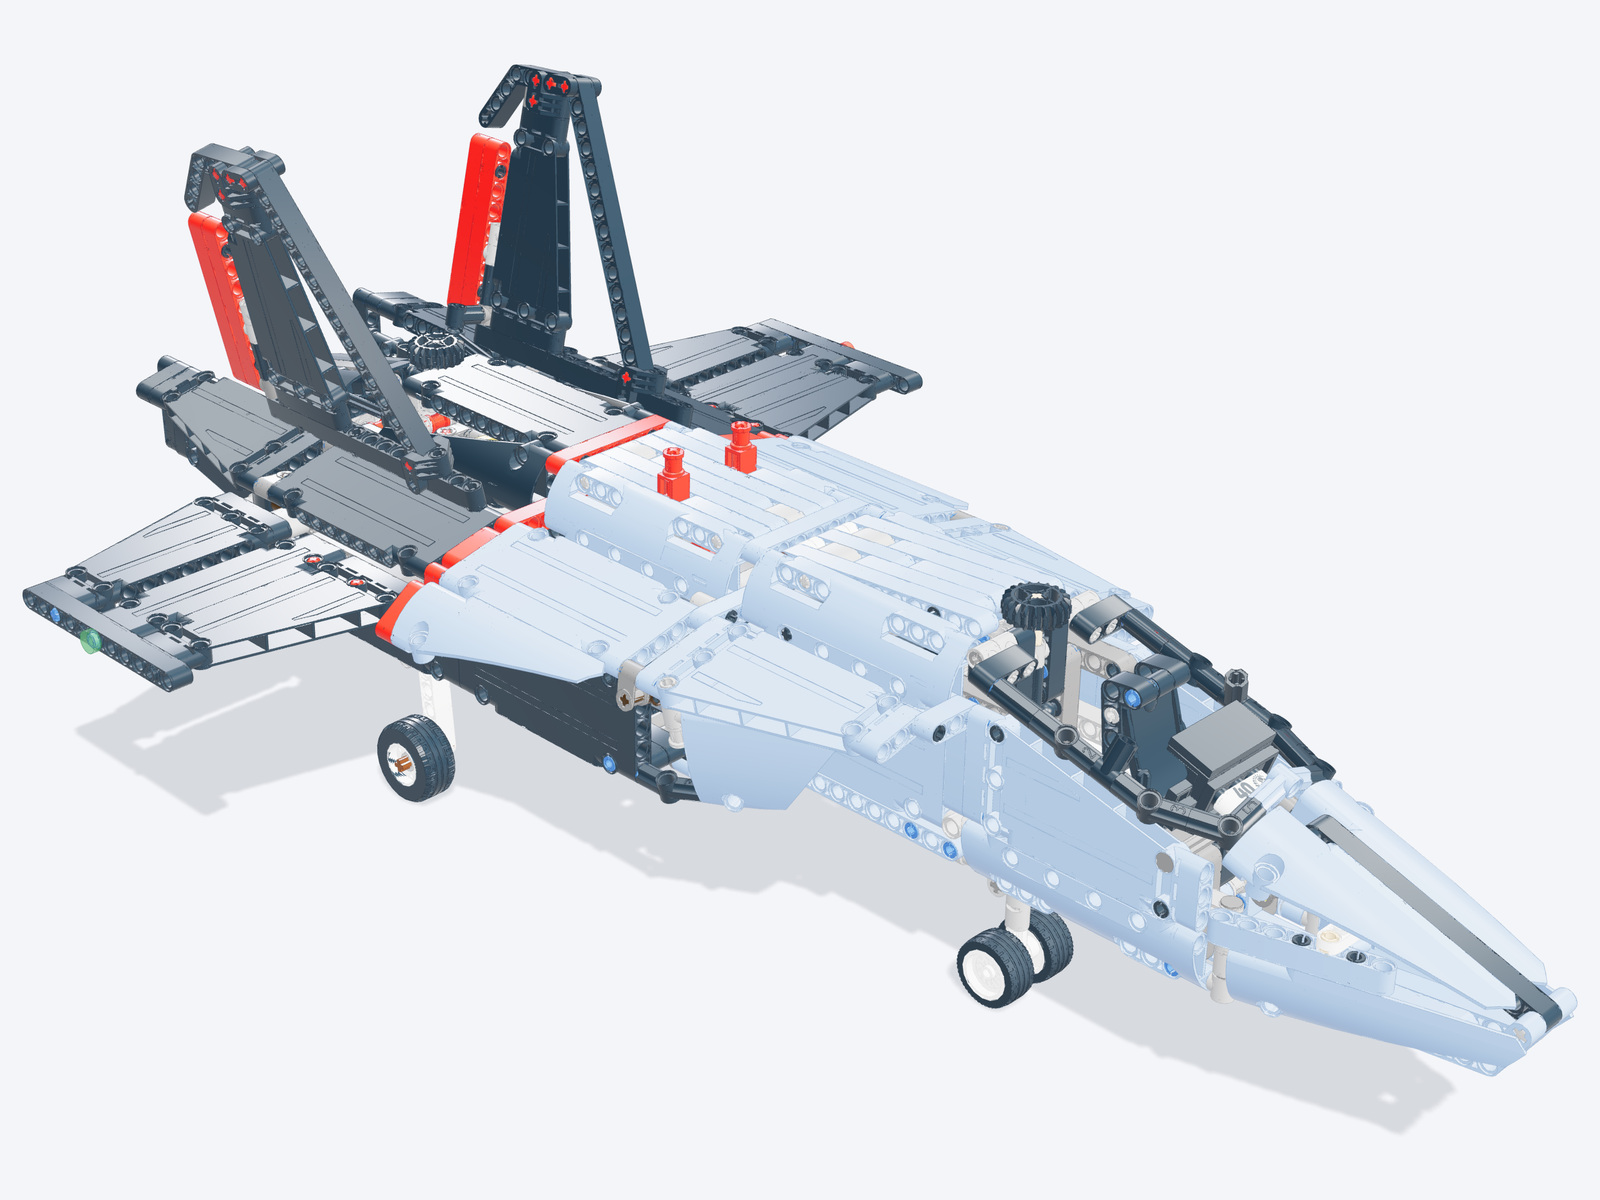
\includegraphics[width=.65\linewidth]{figures-v2/omr-42066-iso.jpg}\end{center}
\paragraph{Attribution.}Philippe Hurbain [Philo]. CC BY 2.0.\par\url{https://library.ldraw.org/library/omr/42066-1.mpd}
\paragraph{Source SHA256.}\path{d1463b1464a83d54a6ed372fba732eabaf79b3857185f4ab60b314e741caa067}
\paragraph{Connector records.}stud: 32; axle: 1534; hinge: 4; fixed: 8; ball: 8
\paragraph{Public input lock.}\path{45366a7ebcd1ddbb144cda3c8ebd441e3d177e2893d9f7a41c43be8d4cfc61fb}
\paragraph{Status.}Source preservation does not certify stability. Reference outputs below are internal review material. Full model inputs are the versioned public JSON and numbered PNGs.
\begin{enumerate}
\item \textbf{ld2-omr-42066-color-1}. Identify the original color of B1144; numbered isolation is allowed.
\par{\small color; visual; atomic; single-choice.\par\textit{Operands:} B1144 = brick\_001144\par\textit{Public evidence summary:} Numbered PNG: benchmark/ldraw-v2/inputs/views/ld2-omr-42066-color-1.png; structured input = \{\}.\par\textit{Options:} A: Blue; B: White; C: Yellow; D: Black\par\textit{Reference output:} \{"choiceId": "D"\}\par\textit{Derivation:} source colorName by rendered B-label; source oracle only\par\textit{Equivalence:} exact declared response\par\textit{Review:} pending required human review.}
\item \textbf{ld2-omr-42066-shape-match-1}. Ignoring color and pose, which numbered instance has the same LDraw part type as B1144?
\par{\small shape-match; visual; atomic; single-choice.\par\textit{Operands:} B0739 = brick\_000739, B1144 = brick\_001144, B0576 = brick\_000576, B0405 = brick\_000405, B0546 = brick\_000546\par\textit{Public evidence summary:} Numbered PNG: benchmark/ldraw-v2/inputs/views/ld2-omr-42066-shape-match-1.png; structured input = \{\}.\par\textit{Options:} A: B0576; B: B0739; C: B0405; D: B0546\par\textit{Reference output:} \{"choiceId": "C"\}\par\textit{Derivation:} source partNumber equality across labeled candidates; source oracle only\par\textit{Equivalence:} same source partNumber; ignore color and pose; perceptual equivalence pending\par\textit{Review:} pending required human review.}
\item \textbf{ld2-omr-42066-distance-1}. Using the supplied geometry bounding-box centers, which candidate is nearest to B1144?
\par{\small distance; source-data; atomic; single-choice.\par\textit{Operands:} B1226 = brick\_001226, B1144 = brick\_001144, B0947 = brick\_000947, B0240 = brick\_000240\par\textit{Public evidence summary:} \{"coordinateFrame": "Viewer world, millimeters, Euclidean distance", "centers": \{"B1144": [-47.588, 105.202992, -266.945856], "B1226": [58.8468, 166.972, -189.987204], "B0947": [0, 64.148442, 284.320131], "B0240": [20, 85.6348, 20.876756]\}\}\par\textit{Options:} A: B0240; B: B1226; C: B0947\par\textit{Reference output:} \{"choiceId": "B"\}\par\textit{Derivation:} Euclidean norm from public rounded centers\par\textit{Equivalence:} exact declared response\par\textit{Review:} machine checks passed; no human certification.}
\item \textbf{ld2-omr-42066-color-2}. Identify the original color of B0286; numbered isolation is allowed.
\par{\small color; visual; atomic; single-choice.\par\textit{Operands:} B0286 = brick\_000286\par\textit{Public evidence summary:} Numbered PNG: benchmark/ldraw-v2/inputs/views/ld2-omr-42066-color-2.png; structured input = \{\}.\par\textit{Options:} A: Black; B: Dark Brown; C: Trans Green; D: Trans Red\par\textit{Reference output:} \{"choiceId": "A"\}\par\textit{Derivation:} source colorName by rendered B-label; source oracle only\par\textit{Equivalence:} exact declared response\par\textit{Review:} pending required human review.}
\item \textbf{ld2-omr-42066-shape-match-2}. Ignoring color and pose, which numbered instance has the same LDraw part type as B0286?
\par{\small shape-match; visual; atomic; single-choice.\par\textit{Operands:} B0175 = brick\_000175, B0867 = brick\_000867, B0286 = brick\_000286, B0604 = brick\_000604, B0128 = brick\_000128\par\textit{Public evidence summary:} Numbered PNG: benchmark/ldraw-v2/inputs/views/ld2-omr-42066-shape-match-2.png; structured input = \{\}.\par\textit{Options:} A: B0128; B: B0175; C: B0867; D: B0604\par\textit{Reference output:} \{"choiceId": "A"\}\par\textit{Derivation:} source partNumber equality across labeled candidates; source oracle only\par\textit{Equivalence:} same source partNumber; ignore color and pose; perceptual equivalence pending\par\textit{Review:} pending required human review.}
\item \textbf{ld2-omr-42066-distance-2}. Using the supplied geometry bounding-box centers, which candidate is nearest to B0286?
\par{\small distance; source-data; atomic; single-choice.\par\textit{Operands:} B0964 = brick\_000964, B0757 = brick\_000757, B0286 = brick\_000286, B0584 = brick\_000584\par\textit{Public evidence summary:} \{"coordinateFrame": "Viewer world, millimeters, Euclidean distance", "centers": \{"B0286": [-26, 101.822608, 2.184334], "B0757": [15.9892, 61.5388, 20.5948], "B0964": [15.800047, 98.829629, 261.097606], "B0584": [-16, 131.207349, 129.781993]\}\}\par\textit{Options:} A: B0757; B: B0964; C: B0584\par\textit{Reference output:} \{"choiceId": "A"\}\par\textit{Derivation:} Euclidean norm from public rounded centers\par\textit{Equivalence:} exact declared response\par\textit{Review:} machine checks passed; no human certification.}
\item \textbf{ld2-omr-42066-color-3}. Identify the original color of B0606; numbered isolation is allowed.
\par{\small color; visual; atomic; single-choice.\par\textit{Operands:} B0606 = brick\_000606\par\textit{Public evidence summary:} Numbered PNG: benchmark/ldraw-v2/inputs/views/ld2-omr-42066-color-3.png; structured input = \{\}.\par\textit{Options:} A: Rubber Black; B: Dark Bluish Grey; C: Yellow; D: Blue\par\textit{Reference output:} \{"choiceId": "D"\}\par\textit{Derivation:} source colorName by rendered B-label; source oracle only\par\textit{Equivalence:} exact declared response\par\textit{Review:} pending required human review.}
\item \textbf{ld2-omr-42066-shape-match-3}. Ignoring color and pose, which numbered instance has the same LDraw part type as B0606?
\par{\small shape-match; visual; atomic; single-choice.\par\textit{Operands:} B0606 = brick\_000606, B0435 = brick\_000435, B1052 = brick\_001052, B0302 = brick\_000302, B1082 = brick\_001082\par\textit{Public evidence summary:} Numbered PNG: benchmark/ldraw-v2/inputs/views/ld2-omr-42066-shape-match-3.png; structured input = \{\}.\par\textit{Options:} A: B0302; B: B1082; C: B1052; D: B0435\par\textit{Reference output:} \{"choiceId": "B"\}\par\textit{Derivation:} source partNumber equality across labeled candidates; source oracle only\par\textit{Equivalence:} same source partNumber; ignore color and pose; perceptual equivalence pending\par\textit{Review:} pending required human review.}
\item \textbf{ld2-omr-42066-distance-3}. Using the supplied geometry bounding-box centers, which candidate is nearest to B0606?
\par{\small distance; source-data; atomic; single-choice.\par\textit{Operands:} B0606 = brick\_000606, B1010 = brick\_001010, B0658 = brick\_000658, B1003 = brick\_001003\par\textit{Public evidence summary:} \{"coordinateFrame": "Viewer world, millimeters, Euclidean distance", "centers": \{"B0606": [12.1, 106.503744, 166.636178], "B1010": [-31.6688, 124.275493, 152.61352], "B0658": [40, 85.5388, 28.8768], "B1003": [29.695036, 112.555599, 194.485323]\}\}\par\textit{Options:} A: B1003; B: B0658; C: B1010\par\textit{Reference output:} \{"choiceId": "A"\}\par\textit{Derivation:} Euclidean norm from public rounded centers\par\textit{Equivalence:} exact declared response\par\textit{Review:} machine checks passed; no human certification.}
\item \textbf{ld2-omr-42066-color-4}. Identify the original color of B0478; numbered isolation is allowed.
\par{\small color; visual; atomic; single-choice.\par\textit{Operands:} B0478 = brick\_000478\par\textit{Public evidence summary:} Numbered PNG: benchmark/ldraw-v2/inputs/views/ld2-omr-42066-color-4.png; structured input = \{\}.\par\textit{Options:} A: Tan; B: Light Bluish Grey; C: White; D: Blue\par\textit{Reference output:} \{"choiceId": "D"\}\par\textit{Derivation:} source colorName by rendered B-label; source oracle only\par\textit{Equivalence:} exact declared response\par\textit{Review:} pending required human review.}
\item \textbf{ld2-omr-42066-shape-match-4}. Ignoring color and pose, which numbered instance has the same LDraw part type as B0478?
\par{\small shape-match; visual; atomic; single-choice.\par\textit{Operands:} B0305 = brick\_000305, B0402 = brick\_000402, B1073 = brick\_001073, B0947 = brick\_000947, B0478 = brick\_000478\par\textit{Public evidence summary:} Numbered PNG: benchmark/ldraw-v2/inputs/views/ld2-omr-42066-shape-match-4.png; structured input = \{\}.\par\textit{Options:} A: B1073; B: B0402; C: B0947; D: B0305\par\textit{Reference output:} \{"choiceId": "C"\}\par\textit{Derivation:} source partNumber equality across labeled candidates; source oracle only\par\textit{Equivalence:} same source partNumber; ignore color and pose; perceptual equivalence pending\par\textit{Review:} pending required human review.}
\item \textbf{ld2-omr-42066-distance-4}. Using the supplied geometry bounding-box centers, which candidate is nearest to B0478?
\par{\small distance; source-data; atomic; single-choice.\par\textit{Operands:} B0478 = brick\_000478, B0379 = brick\_000379, B0569 = brick\_000569, B0103 = brick\_000103\par\textit{Public evidence summary:} \{"coordinateFrame": "Viewer world, millimeters, Euclidean distance", "centers": \{"B0478": [16, 59.4268, 204.5888], "B0569": [28, 116.1948, 141.2608], "B0379": [-24, 110.8828, -82.8352], "B0103": [-29.50087, 89.069647, -28.56805]\}\}\par\textit{Options:} A: B0569; B: B0103; C: B0379\par\textit{Reference output:} \{"choiceId": "A"\}\par\textit{Derivation:} Euclidean norm from public rounded centers\par\textit{Equivalence:} exact declared response\par\textit{Review:} pending required human review.}
\item \textbf{ld2-omr-42066-color-5}. Identify the original color of B0644; numbered isolation is allowed.
\par{\small color; visual; atomic; single-choice.\par\textit{Operands:} B0644 = brick\_000644\par\textit{Public evidence summary:} Numbered PNG: benchmark/ldraw-v2/inputs/views/ld2-omr-42066-color-5.png; structured input = \{\}.\par\textit{Options:} A: Medium Blue; B: Dark Brown; C: Light Bluish Grey; D: Yellow\par\textit{Reference output:} \{"choiceId": "C"\}\par\textit{Derivation:} source colorName by rendered B-label; source oracle only\par\textit{Equivalence:} exact declared response\par\textit{Review:} pending required human review.}
\item \textbf{ld2-omr-42066-shape-match-5}. Ignoring color and pose, which numbered instance has the same LDraw part type as B0644?
\par{\small shape-match; visual; atomic; single-choice.\par\textit{Operands:} B0352 = brick\_000352, B0566 = brick\_000566, B0744 = brick\_000744, B0644 = brick\_000644, B0945 = brick\_000945\par\textit{Public evidence summary:} Numbered PNG: benchmark/ldraw-v2/inputs/views/ld2-omr-42066-shape-match-5.png; structured input = \{\}.\par\textit{Options:} A: B0945; B: B0352; C: B0566; D: B0744\par\textit{Reference output:} \{"choiceId": "A"\}\par\textit{Derivation:} source partNumber equality across labeled candidates; source oracle only\par\textit{Equivalence:} same source partNumber; ignore color and pose; perceptual equivalence pending\par\textit{Review:} pending required human review.}
\item \textbf{ld2-omr-42066-distance-5}. Using the supplied geometry bounding-box centers, which candidate is nearest to B0644?
\par{\small distance; source-data; atomic; single-choice.\par\textit{Operands:} B1071 = brick\_001071, B0306 = brick\_000306, B0644 = brick\_000644, B0074 = brick\_000074\par\textit{Public evidence summary:} \{"coordinateFrame": "Viewer world, millimeters, Euclidean distance", "centers": \{"B0644": [24, 59.2348, 216.398877], "B0306": [-44.4, 79.183139, -81.276917], "B1071": [0.0008, 133.7308, 13.4528], "B0074": [-24, 68.845746, -90.005559]\}\}\par\textit{Options:} A: B0074; B: B0306; C: B1071\par\textit{Reference output:} \{"choiceId": "C"\}\par\textit{Derivation:} Euclidean norm from public rounded centers\par\textit{Equivalence:} exact declared response\par\textit{Review:} pending required human review.}
\item \textbf{ld2-omr-42066-interface-1}. Classify the supplied connector record for B0785 and B0786. This does not certify load capacity.
\par{\small interface; connector-graph; metacognitive; single-choice.\par\textit{Operands:} B0785 = brick\_000785, B0786 = brick\_000786\par\textit{Public evidence summary:} \{"connectorRecord": \{"family": "axle", "aConnector": 0, "bConnector": 0\}, "scope": "Upstream connector tolerances and inset mesh intersections; unknown parts remain explicit, separate scene objects are not glued together; no load/force validation."\}\par\textit{Options:} A: hinge; B: stud; C: ball; D: fixed; E: axle\par\textit{Reference output:} \{"choiceId": "E"\}\par\textit{Derivation:} public connectorRecord.family equality\par\textit{Equivalence:} exact declared response\par\textit{Review:} machine checks passed; no human certification.}
\item \textbf{ld2-omr-42066-interface-2}. Classify the supplied connector record for B0692 and B0694. This does not certify load capacity.
\par{\small interface; connector-graph; metacognitive; single-choice.\par\textit{Operands:} B0694 = brick\_000694, B0692 = brick\_000692\par\textit{Public evidence summary:} \{"connectorRecord": \{"family": "ball", "aConnector": 1, "bConnector": 0\}, "scope": "Upstream connector tolerances and inset mesh intersections; unknown parts remain explicit, separate scene objects are not glued together; no load/force validation."\}\par\textit{Options:} A: hinge; B: fixed; C: ball; D: axle; E: stud\par\textit{Reference output:} \{"choiceId": "C"\}\par\textit{Derivation:} public connectorRecord.family equality\par\textit{Equivalence:} exact declared response\par\textit{Review:} machine checks passed; no human certification.}
\item \textbf{ld2-omr-42066-interface-3}. Classify the supplied connector record for B0413 and B0414. This does not certify load capacity.
\par{\small interface; connector-graph; metacognitive; single-choice.\par\textit{Operands:} B0413 = brick\_000413, B0414 = brick\_000414\par\textit{Public evidence summary:} \{"connectorRecord": \{"family": "fixed", "aConnector": 1, "bConnector": 1\}, "scope": "Upstream connector tolerances and inset mesh intersections; unknown parts remain explicit, separate scene objects are not glued together; no load/force validation."\}\par\textit{Options:} A: axle; B: hinge; C: fixed; D: ball; E: stud\par\textit{Reference output:} \{"choiceId": "C"\}\par\textit{Derivation:} public connectorRecord.family equality\par\textit{Equivalence:} exact declared response\par\textit{Review:} machine checks passed; no human certification.}
\item \textbf{ld2-omr-42066-interface-4}. Classify the supplied connector record for B0553 and B0551. This does not certify load capacity.
\par{\small interface; connector-graph; metacognitive; single-choice.\par\textit{Operands:} B0553 = brick\_000553, B0551 = brick\_000551\par\textit{Public evidence summary:} \{"connectorRecord": \{"family": "hinge", "aConnector": 0, "bConnector": 1\}, "scope": "Upstream connector tolerances and inset mesh intersections; unknown parts remain explicit, separate scene objects are not glued together; no load/force validation."\}\par\textit{Options:} A: stud; B: fixed; C: hinge; D: axle; E: ball\par\textit{Reference output:} \{"choiceId": "C"\}\par\textit{Derivation:} public connectorRecord.family equality\par\textit{Equivalence:} exact declared response\par\textit{Review:} machine checks passed; no human certification.}
\item \textbf{ld2-omr-42066-interface-5}. Classify the supplied connector record for B0988 and B0994. This does not certify load capacity.
\par{\small interface; connector-graph; metacognitive; single-choice.\par\textit{Operands:} B0994 = brick\_000994, B0988 = brick\_000988\par\textit{Public evidence summary:} \{"connectorRecord": \{"family": "stud", "aConnector": 8, "bConnector": 2\}, "scope": "Upstream connector tolerances and inset mesh intersections; unknown parts remain explicit, separate scene objects are not glued together; no load/force validation."\}\par\textit{Options:} A: ball; B: axle; C: stud; D: fixed; E: hinge\par\textit{Reference output:} \{"choiceId": "C"\}\par\textit{Derivation:} public connectorRecord.family equality\par\textit{Equivalence:} exact declared response\par\textit{Review:} machine checks passed; no human certification.}
\item \textbf{ld2-omr-42066-neighbors-1}. Select every candidate directly adjacent to B1156 in the supplied connector graph.
\par{\small neighbors; connector-graph; metacognitive; multiple-choice.\par\textit{Operands:} B0368 = brick\_000368, B1156 = brick\_001156, B1123 = brick\_001123, B1157 = brick\_001157, B1145 = brick\_001145\par\textit{Public evidence summary:} 2 unique undirected pairs\par\textit{Options:} A: B0368; B: B1157; C: B1123; D: B1145\par\textit{Reference output:} \{"choiceIds": ["B", "D"]\}\par\textit{Derivation:} public incident edge endpoint set\par\textit{Equivalence:} unordered exact set; duplicate IDs invalid\par\textit{Review:} machine checks passed; no human certification.}
\item \textbf{ld2-omr-42066-graph-removal-1}. Delete B1156 and its incident edges from this local graph. How many connected components remain? Do not infer physical extractability.
\par{\small graph-removal; connector-graph; graph-internal; integer.\par\textit{Operands:} B1145 = brick\_001145, B1123 = brick\_001123, B0368 = brick\_000368, B1156 = brick\_001156, B1157 = brick\_001157\par\textit{Public evidence summary:} 2 unique undirected pairs; 5 nodes\par\textit{Reference output:} \{"value": 4\}\par\textit{Derivation:} union-find component count after public target deletion\par\textit{Equivalence:} exact declared response\par\textit{Review:} machine checks passed; no human certification.}
\item \textbf{ld2-omr-42066-neighbors-2}. Select every candidate directly adjacent to B0916 in the supplied connector graph.
\par{\small neighbors; connector-graph; metacognitive; multiple-choice.\par\textit{Operands:} B0176 = brick\_000176, B0426 = brick\_000426, B0916 = brick\_000916, B0824 = brick\_000824, B0915 = brick\_000915\par\textit{Public evidence summary:} 2 unique undirected pairs\par\textit{Options:} A: B0824; B: B0426; C: B0176; D: B0915\par\textit{Reference output:} \{"choiceIds": ["B", "D"]\}\par\textit{Derivation:} public incident edge endpoint set\par\textit{Equivalence:} unordered exact set; duplicate IDs invalid\par\textit{Review:} pending required human review.}
\item \textbf{ld2-omr-42066-graph-removal-2}. Delete B0916 and its incident edges from this local graph. How many connected components remain? Do not infer physical extractability.
\par{\small graph-removal; connector-graph; graph-internal; integer.\par\textit{Operands:} B0915 = brick\_000915, B0426 = brick\_000426, B0916 = brick\_000916, B0824 = brick\_000824, B0176 = brick\_000176\par\textit{Public evidence summary:} 2 unique undirected pairs; 5 nodes\par\textit{Reference output:} \{"value": 4\}\par\textit{Derivation:} union-find component count after public target deletion\par\textit{Equivalence:} exact declared response\par\textit{Review:} pending required human review.}
\item \textbf{ld2-omr-42066-neighbors-3}. Select every candidate directly adjacent to B1244 in the supplied connector graph.
\par{\small neighbors; connector-graph; metacognitive; multiple-choice.\par\textit{Operands:} B1243 = brick\_001243, B0583 = brick\_000583, B1242 = brick\_001242, B1244 = brick\_001244, B0013 = brick\_000013\par\textit{Public evidence summary:} 2 unique undirected pairs\par\textit{Options:} A: B0583; B: B0013; C: B1242; D: B1243\par\textit{Reference output:} \{"choiceIds": ["C", "D"]\}\par\textit{Derivation:} public incident edge endpoint set\par\textit{Equivalence:} unordered exact set; duplicate IDs invalid\par\textit{Review:} machine checks passed; no human certification.}
\item \textbf{ld2-omr-42066-graph-removal-3}. Delete B1244 and its incident edges from this local graph. How many connected components remain? Do not infer physical extractability.
\par{\small graph-removal; connector-graph; graph-internal; integer.\par\textit{Operands:} B1243 = brick\_001243, B1242 = brick\_001242, B1244 = brick\_001244, B0013 = brick\_000013, B0583 = brick\_000583\par\textit{Public evidence summary:} 2 unique undirected pairs; 5 nodes\par\textit{Reference output:} \{"value": 4\}\par\textit{Derivation:} union-find component count after public target deletion\par\textit{Equivalence:} exact declared response\par\textit{Review:} machine checks passed; no human certification.}
\item \textbf{ld2-omr-42066-neighbors-4}. Select every candidate directly adjacent to B0962 in the supplied connector graph.
\par{\small neighbors; connector-graph; metacognitive; multiple-choice.\par\textit{Operands:} B0960 = brick\_000960, B0847 = brick\_000847, B1087 = brick\_001087, B0962 = brick\_000962, B0961 = brick\_000961\par\textit{Public evidence summary:} 2 unique undirected pairs\par\textit{Options:} A: B0961; B: B0960; C: B0847; D: B1087\par\textit{Reference output:} \{"choiceIds": ["A", "B"]\}\par\textit{Derivation:} public incident edge endpoint set\par\textit{Equivalence:} unordered exact set; duplicate IDs invalid\par\textit{Review:} machine checks passed; no human certification.}
\item \textbf{ld2-omr-42066-graph-removal-4}. Delete B0962 and its incident edges from this local graph. How many connected components remain? Do not infer physical extractability.
\par{\small graph-removal; connector-graph; graph-internal; integer.\par\textit{Operands:} B0847 = brick\_000847, B1087 = brick\_001087, B0961 = brick\_000961, B0960 = brick\_000960, B0962 = brick\_000962\par\textit{Public evidence summary:} 2 unique undirected pairs; 5 nodes\par\textit{Reference output:} \{"value": 4\}\par\textit{Derivation:} union-find component count after public target deletion\par\textit{Equivalence:} exact declared response\par\textit{Review:} machine checks passed; no human certification.}
\item \textbf{ld2-omr-42066-neighbors-5}. Select every candidate directly adjacent to B1003 in the supplied connector graph.
\par{\small neighbors; connector-graph; metacognitive; multiple-choice.\par\textit{Operands:} B1005 = brick\_001005, B0769 = brick\_000769, B1003 = brick\_001003, B0741 = brick\_000741, B1001 = brick\_001001\par\textit{Public evidence summary:} 2 unique undirected pairs\par\textit{Options:} A: B1005; B: B1001; C: B0741; D: B0769\par\textit{Reference output:} \{"choiceIds": ["A", "B"]\}\par\textit{Derivation:} public incident edge endpoint set\par\textit{Equivalence:} unordered exact set; duplicate IDs invalid\par\textit{Review:} machine checks passed; no human certification.}
\item \textbf{ld2-omr-42066-graph-removal-5}. Delete B1003 and its incident edges from this local graph. How many connected components remain? Do not infer physical extractability.
\par{\small graph-removal; connector-graph; graph-internal; integer.\par\textit{Operands:} B1001 = brick\_001001, B0769 = brick\_000769, B1005 = brick\_001005, B0741 = brick\_000741, B1003 = brick\_001003\par\textit{Public evidence summary:} 2 unique undirected pairs; 5 nodes\par\textit{Reference output:} \{"value": 4\}\par\textit{Derivation:} union-find component count after public target deletion\par\textit{Equivalence:} exact declared response\par\textit{Review:} machine checks passed; no human certification.}
\item \textbf{ld2-omr-42066-coverage-1}. Which numbered instance lacks a connector definition in the coverage record, so this audit cannot establish that it is floating?
\par{\small coverage; source-data; metacognitive; single-choice.\par\textit{Operands:} B0025 = brick\_000025, B0286 = brick\_000286, B1144 = brick\_001144, B0606 = brick\_000606\par\textit{Public evidence summary:} \{"coverage": [\{"label": "B1144", "supported": true\}, \{"label": "B0025", "supported": false\}, \{"label": "B0606", "supported": true\}, \{"label": "B0286", "supported": true\}]\}\par\textit{Options:} A: B0606; B: B0286; C: B1144; D: B0025\par\textit{Reference output:} \{"choiceId": "D"\}\par\textit{Derivation:} public supported=false record\par\textit{Equivalence:} exact declared response\par\textit{Review:} pending required human review.}
\item \textbf{ld2-omr-42066-evidence-limit-1}. Only source geometry, connector matching and mesh intersection audits are available. Without mass, friction, material or dynamic tests, is gravitational stability established?
\par{\small evidence-limit; source-data; metacognitive; single-choice.\par\textit{Operands:} none\par\textit{Public evidence summary:} \{"available": ["Original CAD", "Connector inference", "Inset-mesh intersection candidates"]\}\par\textit{Options:} A: Established; B: Not established by this evidence\par\textit{Reference output:} \{"choiceId": "B"\}\par\textit{Derivation:} fixed epistemic control label\par\textit{Equivalence:} exact declared response\par\textit{Review:} machine checks passed; no human certification.}
\item \textbf{ld2-omr-42066-source-step-1}. At which expanded author step does B0163 first appear in the supplied source-step table? Source order is not a collision-free assembly proof.
\par{\small source-step; source-data; procedural; single-choice.\par\textit{Operands:} B0163 = brick\_000163, B0001 = brick\_000001\par\textit{Public evidence summary:} 2 supplied author-step records; exact table in public JSON\par\textit{Options:} A: 1; B: 2; C: 13; D: 40\par\textit{Reference output:} \{"choiceId": "C"\}\par\textit{Derivation:} minimum public step index containing target\par\textit{Equivalence:} exact declared response\par\textit{Review:} pending required human review.}
\item \textbf{ld2-omr-42066-source-step-2}. At which expanded author step does B0709 first appear in the supplied source-step table? Source order is not a collision-free assembly proof.
\par{\small source-step; source-data; procedural; single-choice.\par\textit{Operands:} B0709 = brick\_000709, B0001 = brick\_000001\par\textit{Public evidence summary:} 2 supplied author-step records; exact table in public JSON\par\textit{Options:} A: 9; B: 57; C: 73; D: 14\par\textit{Reference output:} \{"choiceId": "C"\}\par\textit{Derivation:} minimum public step index containing target\par\textit{Equivalence:} exact declared response\par\textit{Review:} machine checks passed; no human certification.}
\item \textbf{ld2-omr-42066-source-step-3}. At which expanded author step does B0804 first appear in the supplied source-step table? Source order is not a collision-free assembly proof.
\par{\small source-step; source-data; procedural; single-choice.\par\textit{Operands:} B0804 = brick\_000804, B0001 = brick\_000001\par\textit{Public evidence summary:} 2 supplied author-step records; exact table in public JSON\par\textit{Options:} A: 112; B: 84; C: 130; D: 91\par\textit{Reference output:} \{"choiceId": "B"\}\par\textit{Derivation:} minimum public step index containing target\par\textit{Equivalence:} exact declared response\par\textit{Review:} machine checks passed; no human certification.}
\item \textbf{ld2-omr-42066-source-step-4}. At which expanded author step does B1237 first appear in the supplied source-step table? Source order is not a collision-free assembly proof.
\par{\small source-step; source-data; procedural; single-choice.\par\textit{Operands:} B0001 = brick\_000001, B1237 = brick\_001237\par\textit{Public evidence summary:} 2 supplied author-step records; exact table in public JSON\par\textit{Options:} A: 95; B: 77; C: 141; D: 134\par\textit{Reference output:} \{"choiceId": "C"\}\par\textit{Derivation:} minimum public step index containing target\par\textit{Equivalence:} exact declared response\par\textit{Review:} machine checks passed; no human certification.}
\item \textbf{ld2-omr-42066-source-step-5}. At which expanded author step does B1173 first appear in the supplied source-step table? Source order is not a collision-free assembly proof.
\par{\small source-step; source-data; procedural; single-choice.\par\textit{Operands:} B0001 = brick\_000001, B1173 = brick\_001173\par\textit{Public evidence summary:} 2 supplied author-step records; exact table in public JSON\par\textit{Options:} A: 76; B: 28; C: 8; D: 133\par\textit{Reference output:} \{"choiceId": "D"\}\par\textit{Derivation:} minimum public step index containing target\par\textit{Equivalence:} exact declared response\par\textit{Review:} machine checks passed; no human certification.}
\item \textbf{ld2-omr-42066-source-sequence-1}. Reveal the supplied source-step window in author order. Actions change visibility only, without simulating insertion trajectories.
\par{\small source-sequence; scene-edit; procedural; actions.\par\textit{Operands:} B0045 = brick\_000045, B0044 = brick\_000044, B0092 = brick\_000092, B0040 = brick\_000040, B0024 = brick\_000024, B0008 = brick\_000008, B0031 = brick\_000031, B0015 = brick\_000015, B0116 = brick\_000116, B0025 = brick\_000025, B0039 = brick\_000039, B0041 = brick\_000041, B0109 = brick\_000109, B0078 = brick\_000078, B0080 = brick\_000080, B0023 = brick\_000023, B0014 = brick\_000014, B0048 = brick\_000048, B0006 = brick\_000006, B0065 = brick\_000065, B0067 = brick\_000067, B0118 = brick\_000118, B0114 = brick\_000114, B0121 = brick\_000121, B0087 = brick\_000087, B0091 = brick\_000091, B0020 = brick\_000020, B0032 = brick\_000032, B0062 = brick\_000062, B0098 = brick\_000098, B0051 = brick\_000051, B0016 = brick\_000016, B0117 = brick\_000117, B0103 = brick\_000103, B0113 = brick\_000113, B0094 = brick\_000094, B0110 = brick\_000110, B0104 = brick\_000104, B0002 = brick\_000002, B0012 = brick\_000012, B0111 = brick\_000111, B0079 = brick\_000079, B0095 = brick\_000095, B0090 = brick\_000090, B0030 = brick\_000030, B0082 = brick\_000082, B0052 = brick\_000052, B0066 = brick\_000066, B0077 = brick\_000077, B0021 = brick\_000021, B0057 = brick\_000057, B0055 = brick\_000055, B0083 = brick\_000083, B0099 = brick\_000099, B0035 = brick\_000035, B0033 = brick\_000033, B0072 = brick\_000072, B0013 = brick\_000013, B0043 = brick\_000043, B0038 = brick\_000038, B0120 = brick\_000120, B0076 = brick\_000076, B0019 = brick\_000019, B0100 = brick\_000100, B0108 = brick\_000108, B0101 = brick\_000101, B0017 = brick\_000017, B0027 = brick\_000027, B0074 = brick\_000074, B0018 = brick\_000018, B0059 = brick\_000059, B0119 = brick\_000119, B0004 = brick\_000004, B0029 = brick\_000029, B0084 = brick\_000084, B0093 = brick\_000093, B0046 = brick\_000046, B0028 = brick\_000028, B0070 = brick\_000070, B0063 = brick\_000063, B0056 = brick\_000056, B0005 = brick\_000005, B0096 = brick\_000096, B0088 = brick\_000088, B0064 = brick\_000064, B0053 = brick\_000053, B0047 = brick\_000047, B0003 = brick\_000003, B0037 = brick\_000037, B0097 = brick\_000097, B0011 = brick\_000011, B0107 = brick\_000107, B0081 = brick\_000081, B0102 = brick\_000102, B0115 = brick\_000115, B0026 = brick\_000026, B0001 = brick\_000001, B0061 = brick\_000061, B0071 = brick\_000071, B0042 = brick\_000042, B0112 = brick\_000112, B0105 = brick\_000105, B0075 = brick\_000075, B0007 = brick\_000007, B0010 = brick\_000010, B0069 = brick\_000069, B0073 = brick\_000073, B0036 = brick\_000036, B0009 = brick\_000009, B0068 = brick\_000068, B0054 = brick\_000054, B0060 = brick\_000060, B0089 = brick\_000089, B0034 = brick\_000034, B0049 = brick\_000049, B0022 = brick\_000022, B0085 = brick\_000085, B0058 = brick\_000058, B0106 = brick\_000106, B0086 = brick\_000086, B0050 = brick\_000050\par\textit{Public evidence summary:} 6 public actions; budget 6; \{"initialFacts": ["start"], "goalFacts": ["done-6"], "absentFacts": []\}\par\textit{Reference output:} \{"actionIds": ["step-1", "step-2", "step-3", "step-4", "step-5", "step-6"]\}\par\textit{Derivation:} public precondition solver\par\textit{Equivalence:} any legal sequence reaching all goals within budget; display-only semantics\par\textit{Review:} pending required human review.}
\item \textbf{ld2-omr-42066-restore-instance-1}. The display copy hides B1144. Restore only that numbered instance, preserving all other instances and source poses.
\par{\small restore-instance; scene-edit; procedural; actions.\par\textit{Operands:} B0001 = brick\_000001, B1144 = brick\_001144\par\textit{Public evidence summary:} 2 public actions; budget 1; \{"initialFacts": ["missing-brick\_001144", "present-brick\_000001"], "goalFacts": ["present-brick\_001144", "present-brick\_000001"], "absentFacts": ["missing-brick\_001144"]\}\par\textit{Reference output:} \{"actionIds": ["restore-B1144"]\}\par\textit{Derivation:} public precondition solver\par\textit{Equivalence:} any legal sequence reaching all goals within budget; display-only semantics\par\textit{Review:} machine checks passed; no human certification.}
\item \textbf{ld2-omr-42066-restore-instance-2}. The display copy hides B0286. Restore only that numbered instance, preserving all other instances and source poses.
\par{\small restore-instance; scene-edit; procedural; actions.\par\textit{Operands:} B0001 = brick\_000001, B0286 = brick\_000286\par\textit{Public evidence summary:} 2 public actions; budget 1; \{"initialFacts": ["missing-brick\_000286", "present-brick\_000001"], "goalFacts": ["present-brick\_000286", "present-brick\_000001"], "absentFacts": ["missing-brick\_000286"]\}\par\textit{Reference output:} \{"actionIds": ["restore-B0286"]\}\par\textit{Derivation:} public precondition solver\par\textit{Equivalence:} any legal sequence reaching all goals within budget; display-only semantics\par\textit{Review:} machine checks passed; no human certification.}
\item \textbf{ld2-omr-42066-restore-instance-3}. The display copy hides B0606. Restore only that numbered instance, preserving all other instances and source poses.
\par{\small restore-instance; scene-edit; procedural; actions.\par\textit{Operands:} B0001 = brick\_000001, B0606 = brick\_000606\par\textit{Public evidence summary:} 2 public actions; budget 1; \{"initialFacts": ["missing-brick\_000606", "present-brick\_000001"], "goalFacts": ["present-brick\_000606", "present-brick\_000001"], "absentFacts": ["missing-brick\_000606"]\}\par\textit{Reference output:} \{"actionIds": ["restore-B0606"]\}\par\textit{Derivation:} public precondition solver\par\textit{Equivalence:} any legal sequence reaching all goals within budget; display-only semantics\par\textit{Review:} machine checks passed; no human certification.}
\end{enumerate}
\clearpage\section{10213: Shuttle Adventure}
1254 source instances; 34 tasks; D4 size band. 191 type strings; 21 color codes; 8 unsupported instances; 63 intersection candidates. 0 expanded author steps. Independent reparse: passed.
\begin{center}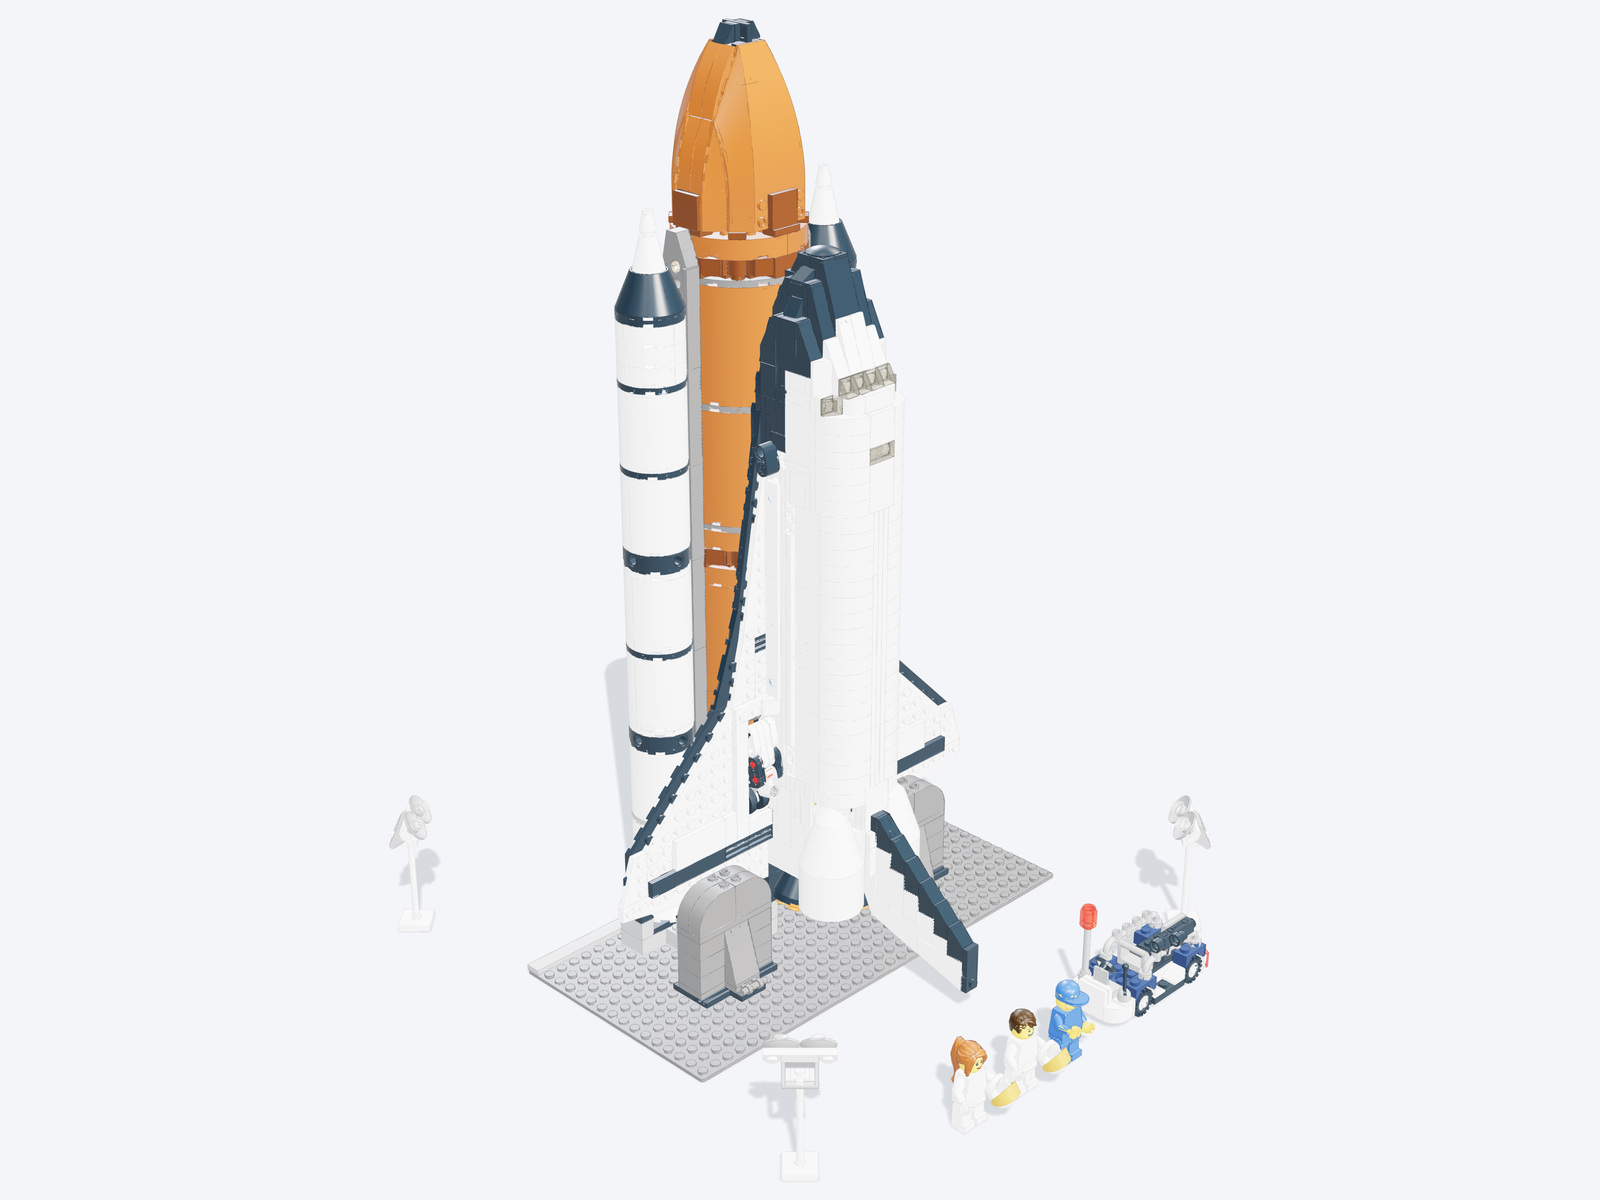
\includegraphics[width=.65\linewidth]{figures-v2/10213-iso.jpg}\end{center}
\paragraph{Attribution.}Edward Carman [EdmanZA]. CC BY 2.0.\par\url{https://library.ldraw.org/omr/sets/870}
\paragraph{Source SHA256.}\path{e295434c8fc8c067e6cd01c398dccd3059a38799f03a6cecddb9319ecf16d909}
\paragraph{Connector records.}stud: 3403; axle: 278; hinge: 35; fixed: 46; ball: 0
\paragraph{Public input lock.}\path{4507454adaa976aa47da6667cc340c69548b3b8358a21db12a1c31b2d33ae60e}
\paragraph{Status.}Source preservation does not certify stability. Reference outputs below are internal review material. Full model inputs are the versioned public JSON and numbered PNGs.
\begin{enumerate}
\item \textbf{ld2-10213-color-1}. Identify the original color of B0957; numbered isolation is allowed.
\par{\small color; visual; atomic; single-choice.\par\textit{Operands:} B0957 = brick\_000957\par\textit{Public evidence summary:} Numbered PNG: benchmark/ldraw-v2/inputs/views/ld2-10213-color-1.png; structured input = \{\}.\par\textit{Options:} A: Trans Brown; B: White; C: Dark Blue; D: Black\par\textit{Reference output:} \{"choiceId": "D"\}\par\textit{Derivation:} source colorName by rendered B-label; source oracle only\par\textit{Equivalence:} exact declared response\par\textit{Review:} pending required human review.}
\item \textbf{ld2-10213-shape-match-1}. Ignoring color and pose, which numbered instance has the same LDraw part type as B0957?
\par{\small shape-match; visual; atomic; single-choice.\par\textit{Operands:} B0137 = brick\_000137, B0893 = brick\_000893, B0957 = brick\_000957, B0249 = brick\_000249, B0782 = brick\_000782\par\textit{Public evidence summary:} Numbered PNG: benchmark/ldraw-v2/inputs/views/ld2-10213-shape-match-1.png; structured input = \{\}.\par\textit{Options:} A: B0782; B: B0893; C: B0137; D: B0249\par\textit{Reference output:} \{"choiceId": "C"\}\par\textit{Derivation:} source partNumber equality across labeled candidates; source oracle only\par\textit{Equivalence:} same source partNumber; ignore color and pose; perceptual equivalence pending\par\textit{Review:} pending required human review.}
\item \textbf{ld2-10213-distance-1}. Using the supplied geometry bounding-box centers, which candidate is nearest to B0957?
\par{\small distance; source-data; atomic; single-choice.\par\textit{Operands:} B0762 = brick\_000762, B0957 = brick\_000957, B0706 = brick\_000706, B0713 = brick\_000713\par\textit{Public evidence summary:} \{"coordinateFrame": "Viewer world, millimeters, Euclidean distance", "centers": \{"B0957": [-4, 297.6, 23.2], "B0713": [-16.1, 237.6, 7.2], "B0706": [0, 113.452, 13.3412], "B0762": [-20, 237.6, 21.6]\}\}\par\textit{Options:} A: B0762; B: B0706; C: B0713\par\textit{Reference output:} \{"choiceId": "A"\}\par\textit{Derivation:} Euclidean norm from public rounded centers\par\textit{Equivalence:} exact declared response\par\textit{Review:} pending required human review.}
\item \textbf{ld2-10213-color-2}. Identify the original color of B0396; numbered isolation is allowed.
\par{\small color; visual; atomic; single-choice.\par\textit{Operands:} B0396 = brick\_000396\par\textit{Public evidence summary:} Numbered PNG: benchmark/ldraw-v2/inputs/views/ld2-10213-color-2.png; structured input = \{\}.\par\textit{Options:} A: Dark Blue; B: Reddish Brown; C: Dark Bluish Grey; D: Light Bluish Grey\par\textit{Reference output:} \{"choiceId": "C"\}\par\textit{Derivation:} source colorName by rendered B-label; source oracle only\par\textit{Equivalence:} exact declared response\par\textit{Review:} pending required human review.}
\item \textbf{ld2-10213-shape-match-2}. Ignoring color and pose, which numbered instance has the same LDraw part type as B0396?
\par{\small shape-match; visual; atomic; single-choice.\par\textit{Operands:} B0388 = brick\_000388, B1086 = brick\_001086, B0268 = brick\_000268, B0396 = brick\_000396, B0469 = brick\_000469\par\textit{Public evidence summary:} Numbered PNG: benchmark/ldraw-v2/inputs/views/ld2-10213-shape-match-2.png; structured input = \{\}.\par\textit{Options:} A: B1086; B: B0268; C: B0469; D: B0388\par\textit{Reference output:} \{"choiceId": "D"\}\par\textit{Derivation:} source partNumber equality across labeled candidates; source oracle only\par\textit{Equivalence:} same source partNumber; ignore color and pose; perceptual equivalence pending\par\textit{Review:} pending required human review.}
\item \textbf{ld2-10213-distance-2}. Using the supplied geometry bounding-box centers, which candidate is nearest to B0396?
\par{\small distance; source-data; atomic; single-choice.\par\textit{Operands:} B0106 = brick\_000106, B0394 = brick\_000394, B0396 = brick\_000396, B1116 = brick\_001116\par\textit{Public evidence summary:} \{"coordinateFrame": "Viewer world, millimeters, Euclidean distance", "centers": \{"B0396": [36, 325.6, -34.4], "B0394": [36, 277.6, -34.4], "B0106": [130.111595, 62.1388, -141.423595], "B1116": [-21.0432, 41.9484, 41.6]\}\}\par\textit{Options:} A: B0106; B: B1116; C: B0394\par\textit{Reference output:} \{"choiceId": "C"\}\par\textit{Derivation:} Euclidean norm from public rounded centers\par\textit{Equivalence:} exact declared response\par\textit{Review:} machine checks passed; no human certification.}
\item \textbf{ld2-10213-color-3}. Identify the original color of B0228; numbered isolation is allowed.
\par{\small color; visual; atomic; single-choice.\par\textit{Operands:} B0228 = brick\_000228\par\textit{Public evidence summary:} Numbered PNG: benchmark/ldraw-v2/inputs/views/ld2-10213-color-3.png; structured input = \{\}.\par\textit{Options:} A: Trans Clear; B: Tan; C: Dark Brown; D: Reddish Brown\par\textit{Reference output:} \{"choiceId": "D"\}\par\textit{Derivation:} source colorName by rendered B-label; source oracle only\par\textit{Equivalence:} exact declared response\par\textit{Review:} pending required human review.}
\item \textbf{ld2-10213-shape-match-3}. Ignoring color and pose, which numbered instance has the same LDraw part type as B0228?
\par{\small shape-match; visual; atomic; single-choice.\par\textit{Operands:} B0921 = brick\_000921, B0237 = brick\_000237, B0228 = brick\_000228, B0303 = brick\_000303, B1084 = brick\_001084\par\textit{Public evidence summary:} Numbered PNG: benchmark/ldraw-v2/inputs/views/ld2-10213-shape-match-3.png; structured input = \{\}.\par\textit{Options:} A: B0237; B: B0921; C: B0303; D: B1084\par\textit{Reference output:} \{"choiceId": "C"\}\par\textit{Derivation:} source partNumber equality across labeled candidates; source oracle only\par\textit{Equivalence:} same source partNumber; ignore color and pose; perceptual equivalence pending\par\textit{Review:} pending required human review.}
\item \textbf{ld2-10213-distance-3}. Using the supplied geometry bounding-box centers, which candidate is nearest to B0228?
\par{\small distance; source-data; atomic; single-choice.\par\textit{Operands:} B0228 = brick\_000228, B0150 = brick\_000150, B0732 = brick\_000732, B1155 = brick\_001155\par\textit{Public evidence summary:} \{"coordinateFrame": "Viewer world, millimeters, Euclidean distance", "centers": \{"B0228": [0, 266.4, -40], "B0150": [-12, 109.6, -15.2], "B0732": [0, 69.7, 23.2], "B1155": [4, 209.6, 15.2]\}\}\par\textit{Options:} A: B0732; B: B1155; C: B0150\par\textit{Reference output:} \{"choiceId": "B"\}\par\textit{Derivation:} Euclidean norm from public rounded centers\par\textit{Equivalence:} exact declared response\par\textit{Review:} machine checks passed; no human certification.}
\item \textbf{ld2-10213-color-4}. Identify the original color of B0987; numbered isolation is allowed.
\par{\small color; visual; atomic; single-choice.\par\textit{Operands:} B0987 = brick\_000987\par\textit{Public evidence summary:} Numbered PNG: benchmark/ldraw-v2/inputs/views/ld2-10213-color-4.png; structured input = \{\}.\par\textit{Options:} A: Blue; B: White; C: Metallic Gold; D: Trans Clear\par\textit{Reference output:} \{"choiceId": "B"\}\par\textit{Derivation:} source colorName by rendered B-label; source oracle only\par\textit{Equivalence:} exact declared response\par\textit{Review:} pending required human review.}
\item \textbf{ld2-10213-shape-match-4}. Ignoring color and pose, which numbered instance has the same LDraw part type as B0987?
\par{\small shape-match; visual; atomic; single-choice.\par\textit{Operands:} B0987 = brick\_000987, B0580 = brick\_000580, B0189 = brick\_000189, B0348 = brick\_000348, B0260 = brick\_000260\par\textit{Public evidence summary:} Numbered PNG: benchmark/ldraw-v2/inputs/views/ld2-10213-shape-match-4.png; structured input = \{\}.\par\textit{Options:} A: B0260; B: B0580; C: B0348; D: B0189\par\textit{Reference output:} \{"choiceId": "C"\}\par\textit{Derivation:} source partNumber equality across labeled candidates; source oracle only\par\textit{Equivalence:} same source partNumber; ignore color and pose; perceptual equivalence pending\par\textit{Review:} pending required human review.}
\item \textbf{ld2-10213-distance-4}. Using the supplied geometry bounding-box centers, which candidate is nearest to B0987?
\par{\small distance; source-data; atomic; single-choice.\par\textit{Operands:} B0987 = brick\_000987, B0260 = brick\_000260, B0588 = brick\_000588, B0146 = brick\_000146\par\textit{Public evidence summary:} \{"coordinateFrame": "Viewer world, millimeters, Euclidean distance", "centers": \{"B0987": [-12, 117.6, 16], "B0588": [44, 109.6, -2.4], "B0146": [-24.8, 109.6, -52], "B0260": [20, 349.6, -20]\}\}\par\textit{Options:} A: B0588; B: B0146; C: B0260\par\textit{Reference output:} \{"choiceId": "A"\}\par\textit{Derivation:} Euclidean norm from public rounded centers\par\textit{Equivalence:} exact declared response\par\textit{Review:} pending required human review.}
\item \textbf{ld2-10213-color-5}. Identify the original color of B0984; numbered isolation is allowed.
\par{\small color; visual; atomic; single-choice.\par\textit{Operands:} B0984 = brick\_000984\par\textit{Public evidence summary:} Numbered PNG: benchmark/ldraw-v2/inputs/views/ld2-10213-color-5.png; structured input = \{\}.\par\textit{Options:} A: Metallic Gold; B: Yellow; C: Trans Red; D: Black\par\textit{Reference output:} \{"choiceId": "D"\}\par\textit{Derivation:} source colorName by rendered B-label; source oracle only\par\textit{Equivalence:} exact declared response\par\textit{Review:} pending required human review.}
\item \textbf{ld2-10213-shape-match-5}. Ignoring color and pose, which numbered instance has the same LDraw part type as B0984?
\par{\small shape-match; visual; atomic; single-choice.\par\textit{Operands:} B1072 = brick\_001072, B0984 = brick\_000984, B0926 = brick\_000926, B0356 = brick\_000356, B0881 = brick\_000881\par\textit{Public evidence summary:} Numbered PNG: benchmark/ldraw-v2/inputs/views/ld2-10213-shape-match-5.png; structured input = \{\}.\par\textit{Options:} A: B1072; B: B0356; C: B0881; D: B0926\par\textit{Reference output:} \{"choiceId": "D"\}\par\textit{Derivation:} source partNumber equality across labeled candidates; source oracle only\par\textit{Equivalence:} same source partNumber; ignore color and pose; perceptual equivalence pending\par\textit{Review:} pending required human review.}
\item \textbf{ld2-10213-distance-5}. Using the supplied geometry bounding-box centers, which candidate is nearest to B0984?
\par{\small distance; source-data; atomic; single-choice.\par\textit{Operands:} B1060 = brick\_001060, B0984 = brick\_000984, B0273 = brick\_000273, B1233 = brick\_001233\par\textit{Public evidence summary:} \{"coordinateFrame": "Viewer world, millimeters, Euclidean distance", "centers": \{"B0984": [-20, 301.6, 4], "B1060": [-20, 300, 22.4], "B0273": [20, 349.6, -28], "B1233": [-30.6, 5.8, 170.8]\}\}\par\textit{Options:} A: B1060; B: B0273; C: B1233\par\textit{Reference output:} \{"choiceId": "A"\}\par\textit{Derivation:} Euclidean norm from public rounded centers\par\textit{Equivalence:} exact declared response\par\textit{Review:} machine checks passed; no human certification.}
\item \textbf{ld2-10213-interface-1}. Classify the supplied connector record for B0645 and B0800. This does not certify load capacity.
\par{\small interface; connector-graph; metacognitive; single-choice.\par\textit{Operands:} B0645 = brick\_000645, B0800 = brick\_000800\par\textit{Public evidence summary:} \{"connectorRecord": \{"family": "axle", "aConnector": 1, "bConnector": 0\}, "scope": "Upstream connector tolerances and inset mesh intersections; unknown parts remain explicit, separate scene objects are not glued together; no load/force validation."\}\par\textit{Options:} A: axle; B: fixed; C: stud; D: ball; E: hinge\par\textit{Reference output:} \{"choiceId": "A"\}\par\textit{Derivation:} public connectorRecord.family equality\par\textit{Equivalence:} exact declared response\par\textit{Review:} machine checks passed; no human certification.}
\item \textbf{ld2-10213-interface-2}. Classify the supplied connector record for B0723 and B0724. This does not certify load capacity.
\par{\small interface; connector-graph; metacognitive; single-choice.\par\textit{Operands:} B0723 = brick\_000723, B0724 = brick\_000724\par\textit{Public evidence summary:} \{"connectorRecord": \{"family": "fixed", "aConnector": 1, "bConnector": 0\}, "scope": "Upstream connector tolerances and inset mesh intersections; unknown parts remain explicit, separate scene objects are not glued together; no load/force validation."\}\par\textit{Options:} A: axle; B: fixed; C: hinge; D: ball; E: stud\par\textit{Reference output:} \{"choiceId": "B"\}\par\textit{Derivation:} public connectorRecord.family equality\par\textit{Equivalence:} exact declared response\par\textit{Review:} machine checks passed; no human certification.}
\item \textbf{ld2-10213-interface-3}. Classify the supplied connector record for B1248 and B1244. This does not certify load capacity.
\par{\small interface; connector-graph; metacognitive; single-choice.\par\textit{Operands:} B1248 = brick\_001248, B1244 = brick\_001244\par\textit{Public evidence summary:} \{"connectorRecord": \{"family": "hinge", "aConnector": 0, "bConnector": 5\}, "scope": "Upstream connector tolerances and inset mesh intersections; unknown parts remain explicit, separate scene objects are not glued together; no load/force validation."\}\par\textit{Options:} A: axle; B: hinge; C: fixed; D: ball; E: stud\par\textit{Reference output:} \{"choiceId": "B"\}\par\textit{Derivation:} public connectorRecord.family equality\par\textit{Equivalence:} exact declared response\par\textit{Review:} machine checks passed; no human certification.}
\item \textbf{ld2-10213-interface-4}. Classify the supplied connector record for B0375 and B0391. This does not certify load capacity.
\par{\small interface; connector-graph; metacognitive; single-choice.\par\textit{Operands:} B0375 = brick\_000375, B0391 = brick\_000391\par\textit{Public evidence summary:} \{"connectorRecord": \{"family": "stud", "aConnector": 68, "bConnector": 9\}, "scope": "Upstream connector tolerances and inset mesh intersections; unknown parts remain explicit, separate scene objects are not glued together; no load/force validation."\}\par\textit{Options:} A: fixed; B: stud; C: axle; D: hinge; E: ball\par\textit{Reference output:} \{"choiceId": "B"\}\par\textit{Derivation:} public connectorRecord.family equality\par\textit{Equivalence:} exact declared response\par\textit{Review:} machine checks passed; no human certification.}
\item \textbf{ld2-10213-neighbors-1}. Select every candidate directly adjacent to B0219 in the supplied connector graph.
\par{\small neighbors; connector-graph; metacognitive; multiple-choice.\par\textit{Operands:} B0446 = brick\_000446, B0178 = brick\_000178, B0191 = brick\_000191, B0984 = brick\_000984, B0219 = brick\_000219, B0196 = brick\_000196, B0224 = brick\_000224, B0181 = brick\_000181, B0187 = brick\_000187\par\textit{Public evidence summary:} 6 unique undirected pairs\par\textit{Options:} A: B0191; B: B0181; C: B0984; D: B0196; E: B0187; F: B0446; G: B0224; H: B0178\par\textit{Reference output:} \{"choiceIds": ["A", "B", "D", "E", "G", "H"]\}\par\textit{Derivation:} public incident edge endpoint set\par\textit{Equivalence:} unordered exact set; duplicate IDs invalid\par\textit{Review:} pending required human review.}
\item \textbf{ld2-10213-graph-removal-1}. Delete B0219 and its incident edges from this local graph. How many connected components remain? Do not infer physical extractability.
\par{\small graph-removal; connector-graph; graph-internal; integer.\par\textit{Operands:} B0446 = brick\_000446, B0196 = brick\_000196, B0224 = brick\_000224, B0984 = brick\_000984, B0178 = brick\_000178, B0191 = brick\_000191, B0181 = brick\_000181, B0219 = brick\_000219, B0187 = brick\_000187\par\textit{Public evidence summary:} 6 unique undirected pairs; 9 nodes\par\textit{Reference output:} \{"value": 8\}\par\textit{Derivation:} union-find component count after public target deletion\par\textit{Equivalence:} exact declared response\par\textit{Review:} pending required human review.}
\item \textbf{ld2-10213-neighbors-2}. Select every candidate directly adjacent to B0487 in the supplied connector graph.
\par{\small neighbors; connector-graph; metacognitive; multiple-choice.\par\textit{Operands:} B0476 = brick\_000476, B0487 = brick\_000487, B0488 = brick\_000488, B1002 = brick\_001002, B0310 = brick\_000310\par\textit{Public evidence summary:} 2 unique undirected pairs\par\textit{Options:} A: B0310; B: B1002; C: B0476; D: B0488\par\textit{Reference output:} \{"choiceIds": ["C", "D"]\}\par\textit{Derivation:} public incident edge endpoint set\par\textit{Equivalence:} unordered exact set; duplicate IDs invalid\par\textit{Review:} machine checks passed; no human certification.}
\item \textbf{ld2-10213-graph-removal-2}. Delete B0487 and its incident edges from this local graph. How many connected components remain? Do not infer physical extractability.
\par{\small graph-removal; connector-graph; graph-internal; integer.\par\textit{Operands:} B0487 = brick\_000487, B0310 = brick\_000310, B1002 = brick\_001002, B0488 = brick\_000488, B0476 = brick\_000476\par\textit{Public evidence summary:} 2 unique undirected pairs; 5 nodes\par\textit{Reference output:} \{"value": 4\}\par\textit{Derivation:} union-find component count after public target deletion\par\textit{Equivalence:} exact declared response\par\textit{Review:} machine checks passed; no human certification.}
\item \textbf{ld2-10213-neighbors-3}. Select every candidate directly adjacent to B0445 in the supplied connector graph.
\par{\small neighbors; connector-graph; metacognitive; multiple-choice.\par\textit{Operands:} B0445 = brick\_000445, B0570 = brick\_000570, B0449 = brick\_000449, B0440 = brick\_000440, B0601 = brick\_000601\par\textit{Public evidence summary:} 2 unique undirected pairs\par\textit{Options:} A: B0440; B: B0570; C: B0601; D: B0449\par\textit{Reference output:} \{"choiceIds": ["A", "D"]\}\par\textit{Derivation:} public incident edge endpoint set\par\textit{Equivalence:} unordered exact set; duplicate IDs invalid\par\textit{Review:} machine checks passed; no human certification.}
\item \textbf{ld2-10213-graph-removal-3}. Delete B0445 and its incident edges from this local graph. How many connected components remain? Do not infer physical extractability.
\par{\small graph-removal; connector-graph; graph-internal; integer.\par\textit{Operands:} B0601 = brick\_000601, B0570 = brick\_000570, B0440 = brick\_000440, B0449 = brick\_000449, B0445 = brick\_000445\par\textit{Public evidence summary:} 2 unique undirected pairs; 5 nodes\par\textit{Reference output:} \{"value": 4\}\par\textit{Derivation:} union-find component count after public target deletion\par\textit{Equivalence:} exact declared response\par\textit{Review:} machine checks passed; no human certification.}
\item \textbf{ld2-10213-neighbors-4}. Select every candidate directly adjacent to B0668 in the supplied connector graph.
\par{\small neighbors; connector-graph; metacognitive; multiple-choice.\par\textit{Operands:} B0759 = brick\_000759, B0418 = brick\_000418, B0672 = brick\_000672, B0669 = brick\_000669, B0668 = brick\_000668\par\textit{Public evidence summary:} 2 unique undirected pairs\par\textit{Options:} A: B0672; B: B0418; C: B0759; D: B0669\par\textit{Reference output:} \{"choiceIds": ["A", "D"]\}\par\textit{Derivation:} public incident edge endpoint set\par\textit{Equivalence:} unordered exact set; duplicate IDs invalid\par\textit{Review:} pending required human review.}
\item \textbf{ld2-10213-graph-removal-4}. Delete B0668 and its incident edges from this local graph. How many connected components remain? Do not infer physical extractability.
\par{\small graph-removal; connector-graph; graph-internal; integer.\par\textit{Operands:} B0759 = brick\_000759, B0672 = brick\_000672, B0669 = brick\_000669, B0418 = brick\_000418, B0668 = brick\_000668\par\textit{Public evidence summary:} 2 unique undirected pairs; 5 nodes\par\textit{Reference output:} \{"value": 4\}\par\textit{Derivation:} union-find component count after public target deletion\par\textit{Equivalence:} exact declared response\par\textit{Review:} pending required human review.}
\item \textbf{ld2-10213-neighbors-5}. Select every candidate directly adjacent to B0007 in the supplied connector graph.
\par{\small neighbors; connector-graph; metacognitive; multiple-choice.\par\textit{Operands:} B0007 = brick\_000007, B0023 = brick\_000023, B0001 = brick\_000001, B0946 = brick\_000946, B1163 = brick\_001163, B0025 = brick\_000025\par\textit{Public evidence summary:} 3 unique undirected pairs\par\textit{Options:} A: B0946; B: B0023; C: B1163; D: B0001; E: B0025\par\textit{Reference output:} \{"choiceIds": ["B", "D", "E"]\}\par\textit{Derivation:} public incident edge endpoint set\par\textit{Equivalence:} unordered exact set; duplicate IDs invalid\par\textit{Review:} pending required human review.}
\item \textbf{ld2-10213-graph-removal-5}. Delete B0007 and its incident edges from this local graph. How many connected components remain? Do not infer physical extractability.
\par{\small graph-removal; connector-graph; graph-internal; integer.\par\textit{Operands:} B0946 = brick\_000946, B0007 = brick\_000007, B0023 = brick\_000023, B0001 = brick\_000001, B0025 = brick\_000025, B1163 = brick\_001163\par\textit{Public evidence summary:} 3 unique undirected pairs; 6 nodes\par\textit{Reference output:} \{"value": 5\}\par\textit{Derivation:} union-find component count after public target deletion\par\textit{Equivalence:} exact declared response\par\textit{Review:} pending required human review.}
\item \textbf{ld2-10213-coverage-1}. Which numbered instance lacks a connector definition in the coverage record, so this audit cannot establish that it is floating?
\par{\small coverage; source-data; metacognitive; single-choice.\par\textit{Operands:} B0396 = brick\_000396, B0957 = brick\_000957, B0706 = brick\_000706, B0228 = brick\_000228\par\textit{Public evidence summary:} \{"coverage": [\{"label": "B0228", "supported": true\}, \{"label": "B0396", "supported": true\}, \{"label": "B0957", "supported": true\}, \{"label": "B0706", "supported": false\}]\}\par\textit{Options:} A: B0957; B: B0228; C: B0396; D: B0706\par\textit{Reference output:} \{"choiceId": "D"\}\par\textit{Derivation:} public supported=false record\par\textit{Equivalence:} exact declared response\par\textit{Review:} pending required human review.}
\item \textbf{ld2-10213-evidence-limit-1}. Only source geometry, connector matching and mesh intersection audits are available. Without mass, friction, material or dynamic tests, is gravitational stability established?
\par{\small evidence-limit; source-data; metacognitive; single-choice.\par\textit{Operands:} none\par\textit{Public evidence summary:} \{"available": ["Original CAD", "Connector inference", "Inset-mesh intersection candidates"]\}\par\textit{Options:} A: Not established by this evidence; B: Established\par\textit{Reference output:} \{"choiceId": "A"\}\par\textit{Derivation:} fixed epistemic control label\par\textit{Equivalence:} exact declared response\par\textit{Review:} machine checks passed; no human certification.}
\item \textbf{ld2-10213-restore-instance-1}. The display copy hides B0957. Restore only that numbered instance, preserving all other instances and source poses.
\par{\small restore-instance; scene-edit; procedural; actions.\par\textit{Operands:} B0001 = brick\_000001, B0957 = brick\_000957\par\textit{Public evidence summary:} 2 public actions; budget 1; \{"initialFacts": ["missing-brick\_000957", "present-brick\_000001"], "goalFacts": ["present-brick\_000957", "present-brick\_000001"], "absentFacts": ["missing-brick\_000957"]\}\par\textit{Reference output:} \{"actionIds": ["restore-B0957"]\}\par\textit{Derivation:} public precondition solver\par\textit{Equivalence:} any legal sequence reaching all goals within budget; display-only semantics\par\textit{Review:} machine checks passed; no human certification.}
\item \textbf{ld2-10213-restore-instance-2}. The display copy hides B0396. Restore only that numbered instance, preserving all other instances and source poses.
\par{\small restore-instance; scene-edit; procedural; actions.\par\textit{Operands:} B0396 = brick\_000396, B0001 = brick\_000001\par\textit{Public evidence summary:} 2 public actions; budget 1; \{"initialFacts": ["missing-brick\_000396", "present-brick\_000001"], "goalFacts": ["present-brick\_000396", "present-brick\_000001"], "absentFacts": ["missing-brick\_000396"]\}\par\textit{Reference output:} \{"actionIds": ["restore-B0396"]\}\par\textit{Derivation:} public precondition solver\par\textit{Equivalence:} any legal sequence reaching all goals within budget; display-only semantics\par\textit{Review:} machine checks passed; no human certification.}
\item \textbf{ld2-10213-restore-instance-3}. The display copy hides B0228. Restore only that numbered instance, preserving all other instances and source poses.
\par{\small restore-instance; scene-edit; procedural; actions.\par\textit{Operands:} B0001 = brick\_000001, B0228 = brick\_000228\par\textit{Public evidence summary:} 2 public actions; budget 1; \{"initialFacts": ["missing-brick\_000228", "present-brick\_000001"], "goalFacts": ["present-brick\_000228", "present-brick\_000001"], "absentFacts": ["missing-brick\_000228"]\}\par\textit{Reference output:} \{"actionIds": ["restore-B0228"]\}\par\textit{Derivation:} public precondition solver\par\textit{Equivalence:} any legal sequence reaching all goals within budget; display-only semantics\par\textit{Review:} machine checks passed; no human certification.}
\end{enumerate}
\clearpage\section{10265: Ford Mustang}
1357 source instances; 40 tasks; D4 size band. 254 type strings; 19 color codes; 10 unsupported instances; 109 intersection candidates. 82 expanded author steps. Independent reparse: passed.
\begin{center}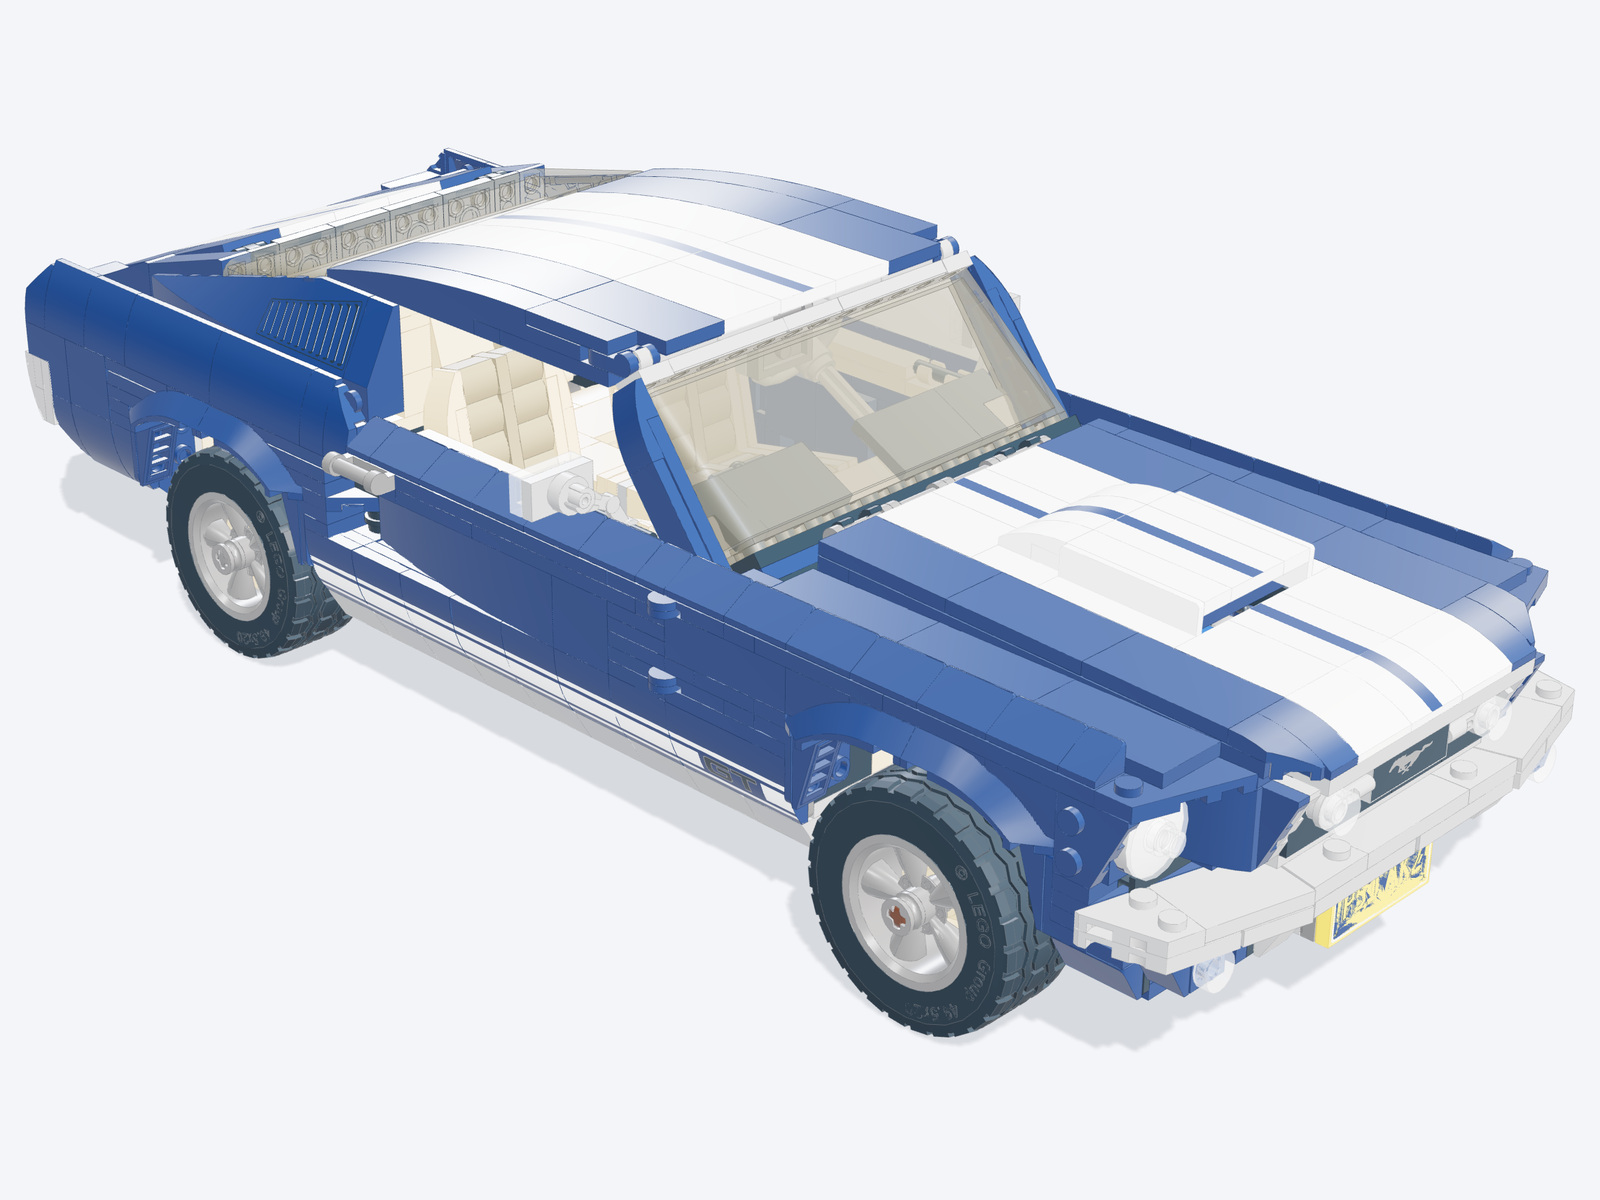
\includegraphics[width=.65\linewidth]{figures-v2/omr-10265-iso.jpg}\end{center}
\paragraph{Attribution.}Ulrich Röder [UR]. CC BY 2.0.\par\url{https://library.ldraw.org/library/omr/10265-1.mpd}
\paragraph{Source SHA256.}\path{e9a2eb1b84d343a6faa9861d186159cf5d1fa1e202366eae1e76287df114ea95}
\paragraph{Connector records.}stud: 3166; axle: 344; hinge: 12; fixed: 0; ball: 4
\paragraph{Public input lock.}\path{40c89a87d4ba0d068bcf063872a92bbaf1f1b5105d03b94158402fda60aa38c2}
\paragraph{Status.}Source preservation does not certify stability. Reference outputs below are internal review material. Full model inputs are the versioned public JSON and numbered PNGs.
\begin{enumerate}
\item \textbf{ld2-omr-10265-color-1}. Identify the original color of B0886; numbered isolation is allowed.
\par{\small color; visual; atomic; single-choice.\par\textit{Operands:} B0886 = brick\_000886\par\textit{Public evidence summary:} Numbered PNG: benchmark/ldraw-v2/inputs/views/ld2-omr-10265-color-1.png; structured input = \{\}.\par\textit{Options:} A: Black; B: Dark Tan; C: Dark Orange; D: Light Bluish Grey\par\textit{Reference output:} \{"choiceId": "D"\}\par\textit{Derivation:} source colorName by rendered B-label; source oracle only\par\textit{Equivalence:} exact declared response\par\textit{Review:} pending required human review.}
\item \textbf{ld2-omr-10265-shape-match-1}. Ignoring color and pose, which numbered instance has the same LDraw part type as B0886?
\par{\small shape-match; visual; atomic; single-choice.\par\textit{Operands:} B0882 = brick\_000882, B0392 = brick\_000392, B0205 = brick\_000205, B0886 = brick\_000886, B0060 = brick\_000060\par\textit{Public evidence summary:} Numbered PNG: benchmark/ldraw-v2/inputs/views/ld2-omr-10265-shape-match-1.png; structured input = \{\}.\par\textit{Options:} A: B0392; B: B0060; C: B0205; D: B0882\par\textit{Reference output:} \{"choiceId": "D"\}\par\textit{Derivation:} source partNumber equality across labeled candidates; source oracle only\par\textit{Equivalence:} same source partNumber; ignore color and pose; perceptual equivalence pending\par\textit{Review:} pending required human review.}
\item \textbf{ld2-omr-10265-distance-1}. Using the supplied geometry bounding-box centers, which candidate is nearest to B0886?
\par{\small distance; source-data; atomic; single-choice.\par\textit{Operands:} B0886 = brick\_000886, B0599 = brick\_000599, B0275 = brick\_000275, B0105 = brick\_000105\par\textit{Public evidence summary:} \{"coordinateFrame": "Viewer world, millimeters, Euclidean distance", "centers": \{"B0886": [59.654664, 31.2, 177.179945], "B0275": [-56, 37.6, 84], "B0105": [56, 50.4, -4], "B0599": [12.1, 21.6, -80]\}\}\par\textit{Options:} A: B0275; B: B0599; C: B0105\par\textit{Reference output:} \{"choiceId": "A"\}\par\textit{Derivation:} Euclidean norm from public rounded centers\par\textit{Equivalence:} exact declared response\par\textit{Review:} machine checks passed; no human certification.}
\item \textbf{ld2-omr-10265-color-2}. Identify the original color of B1090; numbered isolation is allowed.
\par{\small color; visual; atomic; single-choice.\par\textit{Operands:} B1090 = brick\_001090\par\textit{Public evidence summary:} Numbered PNG: benchmark/ldraw-v2/inputs/views/ld2-omr-10265-color-2.png; structured input = \{\}.\par\textit{Options:} A: Tan; B: Trans Red; C: Yellow; D: Aqua\par\textit{Reference output:} \{"choiceId": "A"\}\par\textit{Derivation:} source colorName by rendered B-label; source oracle only\par\textit{Equivalence:} exact declared response\par\textit{Review:} pending required human review.}
\item \textbf{ld2-omr-10265-shape-match-2}. Ignoring color and pose, which numbered instance has the same LDraw part type as B1090?
\par{\small shape-match; visual; atomic; single-choice.\par\textit{Operands:} B0527 = brick\_000527, B1209 = brick\_001209, B1090 = brick\_001090, B0425 = brick\_000425, B1089 = brick\_001089\par\textit{Public evidence summary:} Numbered PNG: benchmark/ldraw-v2/inputs/views/ld2-omr-10265-shape-match-2.png; structured input = \{\}.\par\textit{Options:} A: B0425; B: B1089; C: B0527; D: B1209\par\textit{Reference output:} \{"choiceId": "B"\}\par\textit{Derivation:} source partNumber equality across labeled candidates; source oracle only\par\textit{Equivalence:} same source partNumber; ignore color and pose; perceptual equivalence pending\par\textit{Review:} pending required human review.}
\item \textbf{ld2-omr-10265-distance-2}. Using the supplied geometry bounding-box centers, which candidate is nearest to B1090?
\par{\small distance; source-data; atomic; single-choice.\par\textit{Operands:} B1090 = brick\_001090, B0398 = brick\_000398, B0057 = brick\_000057, B1008 = brick\_001008\par\textit{Public evidence summary:} \{"coordinateFrame": "Viewer world, millimeters, Euclidean distance", "centers": \{"B1090": [48, 56.8, -40], "B0398": [58.32, 21.6, 180], "B0057": [53.6, 24, 24], "B1008": [-27.2, 29.453016, 10.473528]\}\}\par\textit{Options:} A: B0057; B: B1008; C: B0398\par\textit{Reference output:} \{"choiceId": "A"\}\par\textit{Derivation:} Euclidean norm from public rounded centers\par\textit{Equivalence:} exact declared response\par\textit{Review:} machine checks passed; no human certification.}
\item \textbf{ld2-omr-10265-color-3}. Identify the original color of B0079; numbered isolation is allowed.
\par{\small color; visual; atomic; single-choice.\par\textit{Operands:} B0079 = brick\_000079\par\textit{Public evidence summary:} Numbered PNG: benchmark/ldraw-v2/inputs/views/ld2-omr-10265-color-3.png; structured input = \{\}.\par\textit{Options:} A: Aqua; B: Dark Orange; C: Tan; D: Green\par\textit{Reference output:} \{"choiceId": "C"\}\par\textit{Derivation:} source colorName by rendered B-label; source oracle only\par\textit{Equivalence:} exact declared response\par\textit{Review:} pending required human review.}
\item \textbf{ld2-omr-10265-shape-match-3}. Ignoring color and pose, which numbered instance has the same LDraw part type as B0079?
\par{\small shape-match; visual; atomic; single-choice.\par\textit{Operands:} B0269 = brick\_000269, B0311 = brick\_000311, B0759 = brick\_000759, B0079 = brick\_000079, B0283 = brick\_000283\par\textit{Public evidence summary:} Numbered PNG: benchmark/ldraw-v2/inputs/views/ld2-omr-10265-shape-match-3.png; structured input = \{\}.\par\textit{Options:} A: B0759; B: B0283; C: B0311; D: B0269\par\textit{Reference output:} \{"choiceId": "D"\}\par\textit{Derivation:} source partNumber equality across labeled candidates; source oracle only\par\textit{Equivalence:} same source partNumber; ignore color and pose; perceptual equivalence pending\par\textit{Review:} pending required human review.}
\item \textbf{ld2-omr-10265-distance-3}. Using the supplied geometry bounding-box centers, which candidate is nearest to B0079?
\par{\small distance; source-data; atomic; single-choice.\par\textit{Operands:} B1326 = brick\_001326, B0079 = brick\_000079, B0940 = brick\_000940, B1261 = brick\_001261\par\textit{Public evidence summary:} \{"coordinateFrame": "Viewer world, millimeters, Euclidean distance", "centers": \{"B0079": [52, 21.6, 40], "B0940": [20, 32.49576, 70.615832], "B1326": [-48, 34.4, 165.8], "B1261": [-33.524999, 50.4, 116.479116]\}\}\par\textit{Options:} A: B1261; B: B1326; C: B0940\par\textit{Reference output:} \{"choiceId": "C"\}\par\textit{Derivation:} Euclidean norm from public rounded centers\par\textit{Equivalence:} exact declared response\par\textit{Review:} machine checks passed; no human certification.}
\item \textbf{ld2-omr-10265-color-4}. Identify the original color of B0783; numbered isolation is allowed.
\par{\small color; visual; atomic; single-choice.\par\textit{Operands:} B0783 = brick\_000783\par\textit{Public evidence summary:} Numbered PNG: benchmark/ldraw-v2/inputs/views/ld2-omr-10265-color-4.png; structured input = \{\}.\par\textit{Options:} A: Light Bluish Grey; B: Blue; C: Brown; D: Yellow\par\textit{Reference output:} \{"choiceId": "A"\}\par\textit{Derivation:} source colorName by rendered B-label; source oracle only\par\textit{Equivalence:} exact declared response\par\textit{Review:} pending required human review.}
\item \textbf{ld2-omr-10265-shape-match-4}. Ignoring color and pose, which numbered instance has the same LDraw part type as B0783?
\par{\small shape-match; visual; atomic; single-choice.\par\textit{Operands:} B0813 = brick\_000813, B0758 = brick\_000758, B0783 = brick\_000783, B0327 = brick\_000327, B1206 = brick\_001206\par\textit{Public evidence summary:} Numbered PNG: benchmark/ldraw-v2/inputs/views/ld2-omr-10265-shape-match-4.png; structured input = \{\}.\par\textit{Options:} A: B0813; B: B0327; C: B1206; D: B0758\par\textit{Reference output:} \{"choiceId": "D"\}\par\textit{Derivation:} source partNumber equality across labeled candidates; source oracle only\par\textit{Equivalence:} same source partNumber; ignore color and pose; perceptual equivalence pending\par\textit{Review:} pending required human review.}
\item \textbf{ld2-omr-10265-distance-4}. Using the supplied geometry bounding-box centers, which candidate is nearest to B0783?
\par{\small distance; source-data; atomic; single-choice.\par\textit{Operands:} B0157 = brick\_000157, B0783 = brick\_000783, B0683 = brick\_000683, B1240 = brick\_001240\par\textit{Public evidence summary:} \{"coordinateFrame": "Viewer world, millimeters, Euclidean distance", "centers": \{"B0783": [-40, 49.6, 92], "B1240": [40, 52.303984, 68.446956], "B0157": [56, 50.4, 128], "B0683": [-55.92, 12, 40]\}\}\par\textit{Options:} A: B0157; B: B1240; C: B0683\par\textit{Reference output:} \{"choiceId": "C"\}\par\textit{Derivation:} Euclidean norm from public rounded centers\par\textit{Equivalence:} exact declared response\par\textit{Review:} machine checks passed; no human certification.}
\item \textbf{ld2-omr-10265-color-5}. Identify the original color of B1081; numbered isolation is allowed.
\par{\small color; visual; atomic; single-choice.\par\textit{Operands:} B1081 = brick\_001081\par\textit{Public evidence summary:} Numbered PNG: benchmark/ldraw-v2/inputs/views/ld2-omr-10265-color-5.png; structured input = \{\}.\par\textit{Options:} A: Light Grey; B: Dark Blue; C: Dark Bluish Grey; D: Tan\par\textit{Reference output:} \{"choiceId": "C"\}\par\textit{Derivation:} source colorName by rendered B-label; source oracle only\par\textit{Equivalence:} exact declared response\par\textit{Review:} pending required human review.}
\item \textbf{ld2-omr-10265-shape-match-5}. Ignoring color and pose, which numbered instance has the same LDraw part type as B1081?
\par{\small shape-match; visual; atomic; single-choice.\par\textit{Operands:} B0528 = brick\_000528, B1065 = brick\_001065, B1265 = brick\_001265, B1081 = brick\_001081, B0546 = brick\_000546\par\textit{Public evidence summary:} Numbered PNG: benchmark/ldraw-v2/inputs/views/ld2-omr-10265-shape-match-5.png; structured input = \{\}.\par\textit{Options:} A: B1265; B: B1065; C: B0546; D: B0528\par\textit{Reference output:} \{"choiceId": "B"\}\par\textit{Derivation:} source partNumber equality across labeled candidates; source oracle only\par\textit{Equivalence:} same source partNumber; ignore color and pose; perceptual equivalence pending\par\textit{Review:} pending required human review.}
\item \textbf{ld2-omr-10265-distance-5}. Using the supplied geometry bounding-box centers, which candidate is nearest to B1081?
\par{\small distance; source-data; atomic; single-choice.\par\textit{Operands:} B0977 = brick\_000977, B0422 = brick\_000422, B0379 = brick\_000379, B1081 = brick\_001081\par\textit{Public evidence summary:} \{"coordinateFrame": "Viewer world, millimeters, Euclidean distance", "centers": \{"B1081": [-44, 53.6, -80], "B0422": [-24, 85.6, 28], "B0379": [-60.72, 18.4, 168], "B0977": [-24, 54.433218, 54.679544]\}\}\par\textit{Options:} A: B0422; B: B0977; C: B0379\par\textit{Reference output:} \{"choiceId": "A"\}\par\textit{Derivation:} Euclidean norm from public rounded centers\par\textit{Equivalence:} exact declared response\par\textit{Review:} machine checks passed; no human certification.}
\item \textbf{ld2-omr-10265-interface-1}. Classify the supplied connector record for B0013 and B0010. This does not certify load capacity.
\par{\small interface; connector-graph; metacognitive; single-choice.\par\textit{Operands:} B0010 = brick\_000010, B0013 = brick\_000013\par\textit{Public evidence summary:} \{"connectorRecord": \{"family": "axle", "aConnector": 14, "bConnector": 1\}, "scope": "Upstream connector tolerances and inset mesh intersections; unknown parts remain explicit, separate scene objects are not glued together; no load/force validation."\}\par\textit{Options:} A: hinge; B: stud; C: axle; D: ball; E: fixed\par\textit{Reference output:} \{"choiceId": "C"\}\par\textit{Derivation:} public connectorRecord.family equality\par\textit{Equivalence:} exact declared response\par\textit{Review:} pending required human review.}
\item \textbf{ld2-omr-10265-interface-2}. Classify the supplied connector record for B0548 and B0556. This does not certify load capacity.
\par{\small interface; connector-graph; metacognitive; single-choice.\par\textit{Operands:} B0548 = brick\_000548, B0556 = brick\_000556\par\textit{Public evidence summary:} \{"connectorRecord": \{"family": "ball", "aConnector": 3, "bConnector": 7\}, "scope": "Upstream connector tolerances and inset mesh intersections; unknown parts remain explicit, separate scene objects are not glued together; no load/force validation."\}\par\textit{Options:} A: axle; B: stud; C: fixed; D: hinge; E: ball\par\textit{Reference output:} \{"choiceId": "E"\}\par\textit{Derivation:} public connectorRecord.family equality\par\textit{Equivalence:} exact declared response\par\textit{Review:} machine checks passed; no human certification.}
\item \textbf{ld2-omr-10265-interface-3}. Classify the supplied connector record for B0064 and B0065. This does not certify load capacity.
\par{\small interface; connector-graph; metacognitive; single-choice.\par\textit{Operands:} B0064 = brick\_000064, B0065 = brick\_000065\par\textit{Public evidence summary:} \{"connectorRecord": \{"family": "hinge", "aConnector": 1, "bConnector": 2\}, "scope": "Upstream connector tolerances and inset mesh intersections; unknown parts remain explicit, separate scene objects are not glued together; no load/force validation."\}\par\textit{Options:} A: ball; B: hinge; C: axle; D: stud; E: fixed\par\textit{Reference output:} \{"choiceId": "B"\}\par\textit{Derivation:} public connectorRecord.family equality\par\textit{Equivalence:} exact declared response\par\textit{Review:} machine checks passed; no human certification.}
\item \textbf{ld2-omr-10265-interface-4}. Classify the supplied connector record for B0164 and B0165. This does not certify load capacity.
\par{\small interface; connector-graph; metacognitive; single-choice.\par\textit{Operands:} B0164 = brick\_000164, B0165 = brick\_000165\par\textit{Public evidence summary:} \{"connectorRecord": \{"family": "stud", "aConnector": 12, "bConnector": 7\}, "scope": "Upstream connector tolerances and inset mesh intersections; unknown parts remain explicit, separate scene objects are not glued together; no load/force validation."\}\par\textit{Options:} A: stud; B: axle; C: hinge; D: fixed; E: ball\par\textit{Reference output:} \{"choiceId": "A"\}\par\textit{Derivation:} public connectorRecord.family equality\par\textit{Equivalence:} exact declared response\par\textit{Review:} machine checks passed; no human certification.}
\item \textbf{ld2-omr-10265-neighbors-1}. Select every candidate directly adjacent to B0145 in the supplied connector graph.
\par{\small neighbors; connector-graph; metacognitive; multiple-choice.\par\textit{Operands:} B0296 = brick\_000296, B0148 = brick\_000148, B1255 = brick\_001255, B0145 = brick\_000145, B0147 = brick\_000147\par\textit{Public evidence summary:} 2 unique undirected pairs\par\textit{Options:} A: B0296; B: B0147; C: B0148; D: B1255\par\textit{Reference output:} \{"choiceIds": ["B", "C"]\}\par\textit{Derivation:} public incident edge endpoint set\par\textit{Equivalence:} unordered exact set; duplicate IDs invalid\par\textit{Review:} pending required human review.}
\item \textbf{ld2-omr-10265-graph-removal-1}. Delete B0145 and its incident edges from this local graph. How many connected components remain? Do not infer physical extractability.
\par{\small graph-removal; connector-graph; graph-internal; integer.\par\textit{Operands:} B0148 = brick\_000148, B0147 = brick\_000147, B0296 = brick\_000296, B0145 = brick\_000145, B1255 = brick\_001255\par\textit{Public evidence summary:} 2 unique undirected pairs; 5 nodes\par\textit{Reference output:} \{"value": 4\}\par\textit{Derivation:} union-find component count after public target deletion\par\textit{Equivalence:} exact declared response\par\textit{Review:} pending required human review.}
\item \textbf{ld2-omr-10265-neighbors-2}. Select every candidate directly adjacent to B0745 in the supplied connector graph.
\par{\small neighbors; connector-graph; metacognitive; multiple-choice.\par\textit{Operands:} B0740 = brick\_000740, B0367 = brick\_000367, B0751 = brick\_000751, B0772 = brick\_000772, B0745 = brick\_000745\par\textit{Public evidence summary:} 2 unique undirected pairs\par\textit{Options:} A: B0740; B: B0367; C: B0772; D: B0751\par\textit{Reference output:} \{"choiceIds": ["A", "D"]\}\par\textit{Derivation:} public incident edge endpoint set\par\textit{Equivalence:} unordered exact set; duplicate IDs invalid\par\textit{Review:} machine checks passed; no human certification.}
\item \textbf{ld2-omr-10265-graph-removal-2}. Delete B0745 and its incident edges from this local graph. How many connected components remain? Do not infer physical extractability.
\par{\small graph-removal; connector-graph; graph-internal; integer.\par\textit{Operands:} B0751 = brick\_000751, B0367 = brick\_000367, B0745 = brick\_000745, B0740 = brick\_000740, B0772 = brick\_000772\par\textit{Public evidence summary:} 2 unique undirected pairs; 5 nodes\par\textit{Reference output:} \{"value": 4\}\par\textit{Derivation:} union-find component count after public target deletion\par\textit{Equivalence:} exact declared response\par\textit{Review:} machine checks passed; no human certification.}
\item \textbf{ld2-omr-10265-neighbors-3}. Select every candidate directly adjacent to B1252 in the supplied connector graph.
\par{\small neighbors; connector-graph; metacognitive; multiple-choice.\par\textit{Operands:} B1258 = brick\_001258, B0609 = brick\_000609, B1257 = brick\_001257, B1252 = brick\_001252, B0805 = brick\_000805\par\textit{Public evidence summary:} 2 unique undirected pairs\par\textit{Options:} A: B1258; B: B0805; C: B0609; D: B1257\par\textit{Reference output:} \{"choiceIds": ["A", "D"]\}\par\textit{Derivation:} public incident edge endpoint set\par\textit{Equivalence:} unordered exact set; duplicate IDs invalid\par\textit{Review:} pending required human review.}
\item \textbf{ld2-omr-10265-graph-removal-3}. Delete B1252 and its incident edges from this local graph. How many connected components remain? Do not infer physical extractability.
\par{\small graph-removal; connector-graph; graph-internal; integer.\par\textit{Operands:} B1252 = brick\_001252, B0805 = brick\_000805, B1258 = brick\_001258, B1257 = brick\_001257, B0609 = brick\_000609\par\textit{Public evidence summary:} 2 unique undirected pairs; 5 nodes\par\textit{Reference output:} \{"value": 4\}\par\textit{Derivation:} union-find component count after public target deletion\par\textit{Equivalence:} exact declared response\par\textit{Review:} pending required human review.}
\item \textbf{ld2-omr-10265-neighbors-4}. Select every candidate directly adjacent to B1248 in the supplied connector graph.
\par{\small neighbors; connector-graph; metacognitive; multiple-choice.\par\textit{Operands:} B1342 = brick\_001342, B1294 = brick\_001294, B1324 = brick\_001324, B1248 = brick\_001248, B1250 = brick\_001250\par\textit{Public evidence summary:} 2 unique undirected pairs\par\textit{Options:} A: B1342; B: B1250; C: B1294; D: B1324\par\textit{Reference output:} \{"choiceIds": ["A", "B"]\}\par\textit{Derivation:} public incident edge endpoint set\par\textit{Equivalence:} unordered exact set; duplicate IDs invalid\par\textit{Review:} machine checks passed; no human certification.}
\item \textbf{ld2-omr-10265-graph-removal-4}. Delete B1248 and its incident edges from this local graph. How many connected components remain? Do not infer physical extractability.
\par{\small graph-removal; connector-graph; graph-internal; integer.\par\textit{Operands:} B1324 = brick\_001324, B1250 = brick\_001250, B1248 = brick\_001248, B1342 = brick\_001342, B1294 = brick\_001294\par\textit{Public evidence summary:} 2 unique undirected pairs; 5 nodes\par\textit{Reference output:} \{"value": 4\}\par\textit{Derivation:} union-find component count after public target deletion\par\textit{Equivalence:} exact declared response\par\textit{Review:} machine checks passed; no human certification.}
\item \textbf{ld2-omr-10265-neighbors-5}. Select every candidate directly adjacent to B0979 in the supplied connector graph.
\par{\small neighbors; connector-graph; metacognitive; multiple-choice.\par\textit{Operands:} B0979 = brick\_000979, B0980 = brick\_000980, B0719 = brick\_000719, B1133 = brick\_001133, B0964 = brick\_000964\par\textit{Public evidence summary:} 2 unique undirected pairs\par\textit{Options:} A: B0980; B: B0964; C: B0719; D: B1133\par\textit{Reference output:} \{"choiceIds": ["A", "B"]\}\par\textit{Derivation:} public incident edge endpoint set\par\textit{Equivalence:} unordered exact set; duplicate IDs invalid\par\textit{Review:} machine checks passed; no human certification.}
\item \textbf{ld2-omr-10265-graph-removal-5}. Delete B0979 and its incident edges from this local graph. How many connected components remain? Do not infer physical extractability.
\par{\small graph-removal; connector-graph; graph-internal; integer.\par\textit{Operands:} B1133 = brick\_001133, B0980 = brick\_000980, B0979 = brick\_000979, B0719 = brick\_000719, B0964 = brick\_000964\par\textit{Public evidence summary:} 2 unique undirected pairs; 5 nodes\par\textit{Reference output:} \{"value": 4\}\par\textit{Derivation:} union-find component count after public target deletion\par\textit{Equivalence:} exact declared response\par\textit{Review:} machine checks passed; no human certification.}
\item \textbf{ld2-omr-10265-coverage-1}. Which numbered instance lacks a connector definition in the coverage record, so this audit cannot establish that it is floating?
\par{\small coverage; source-data; metacognitive; single-choice.\par\textit{Operands:} B0712 = brick\_000712, B0886 = brick\_000886, B0079 = brick\_000079, B1090 = brick\_001090\par\textit{Public evidence summary:} \{"coverage": [\{"label": "B0886", "supported": true\}, \{"label": "B1090", "supported": true\}, \{"label": "B0079", "supported": true\}, \{"label": "B0712", "supported": false\}]\}\par\textit{Options:} A: B0079; B: B0712; C: B0886; D: B1090\par\textit{Reference output:} \{"choiceId": "B"\}\par\textit{Derivation:} public supported=false record\par\textit{Equivalence:} exact declared response\par\textit{Review:} pending required human review.}
\item \textbf{ld2-omr-10265-evidence-limit-1}. Only source geometry, connector matching and mesh intersection audits are available. Without mass, friction, material or dynamic tests, is gravitational stability established?
\par{\small evidence-limit; source-data; metacognitive; single-choice.\par\textit{Operands:} none\par\textit{Public evidence summary:} \{"available": ["Original CAD", "Connector inference", "Inset-mesh intersection candidates"]\}\par\textit{Options:} A: Not established by this evidence; B: Established\par\textit{Reference output:} \{"choiceId": "A"\}\par\textit{Derivation:} fixed epistemic control label\par\textit{Equivalence:} exact declared response\par\textit{Review:} machine checks passed; no human certification.}
\item \textbf{ld2-omr-10265-source-step-1}. At which expanded author step does B0884 first appear in the supplied source-step table? Source order is not a collision-free assembly proof.
\par{\small source-step; source-data; procedural; single-choice.\par\textit{Operands:} B0884 = brick\_000884, B0001 = brick\_000001\par\textit{Public evidence summary:} 2 supplied author-step records; exact table in public JSON\par\textit{Options:} A: 54; B: 61; C: 66; D: 74\par\textit{Reference output:} \{"choiceId": "A"\}\par\textit{Derivation:} minimum public step index containing target\par\textit{Equivalence:} exact declared response\par\textit{Review:} pending required human review.}
\item \textbf{ld2-omr-10265-source-step-2}. At which expanded author step does B0719 first appear in the supplied source-step table? Source order is not a collision-free assembly proof.
\par{\small source-step; source-data; procedural; single-choice.\par\textit{Operands:} B0719 = brick\_000719, B0001 = brick\_000001\par\textit{Public evidence summary:} 2 supplied author-step records; exact table in public JSON\par\textit{Options:} A: 52; B: 46; C: 34; D: 72\par\textit{Reference output:} \{"choiceId": "B"\}\par\textit{Derivation:} minimum public step index containing target\par\textit{Equivalence:} exact declared response\par\textit{Review:} pending required human review.}
\item \textbf{ld2-omr-10265-source-step-3}. At which expanded author step does B0531 first appear in the supplied source-step table? Source order is not a collision-free assembly proof.
\par{\small source-step; source-data; procedural; single-choice.\par\textit{Operands:} B0531 = brick\_000531, B0001 = brick\_000001\par\textit{Public evidence summary:} 2 supplied author-step records; exact table in public JSON\par\textit{Options:} A: 27; B: 23; C: 7; D: 31\par\textit{Reference output:} \{"choiceId": "D"\}\par\textit{Derivation:} minimum public step index containing target\par\textit{Equivalence:} exact declared response\par\textit{Review:} pending required human review.}
\item \textbf{ld2-omr-10265-source-step-4}. At which expanded author step does B0710 first appear in the supplied source-step table? Source order is not a collision-free assembly proof.
\par{\small source-step; source-data; procedural; single-choice.\par\textit{Operands:} B0001 = brick\_000001, B0710 = brick\_000710\par\textit{Public evidence summary:} 2 supplied author-step records; exact table in public JSON\par\textit{Options:} A: 60; B: 80; C: 45; D: 52\par\textit{Reference output:} \{"choiceId": "C"\}\par\textit{Derivation:} minimum public step index containing target\par\textit{Equivalence:} exact declared response\par\textit{Review:} pending required human review.}
\item \textbf{ld2-omr-10265-source-step-5}. At which expanded author step does B0028 first appear in the supplied source-step table? Source order is not a collision-free assembly proof.
\par{\small source-step; source-data; procedural; single-choice.\par\textit{Operands:} B0028 = brick\_000028, B0001 = brick\_000001\par\textit{Public evidence summary:} 2 supplied author-step records; exact table in public JSON\par\textit{Options:} A: 10; B: 1; C: 6; D: 9\par\textit{Reference output:} \{"choiceId": "A"\}\par\textit{Derivation:} minimum public step index containing target\par\textit{Equivalence:} exact declared response\par\textit{Review:} pending required human review.}
\item \textbf{ld2-omr-10265-source-sequence-1}. Reveal the supplied source-step window in author order. Actions change visibility only, without simulating insertion trajectories.
\par{\small source-sequence; scene-edit; procedural; actions.\par\textit{Operands:} B0018 = brick\_000018, B0005 = brick\_000005, B0008 = brick\_000008, B0001 = brick\_000001, B0017 = brick\_000017, B0006 = brick\_000006, B0011 = brick\_000011, B0010 = brick\_000010, B0009 = brick\_000009, B0012 = brick\_000012, B0003 = brick\_000003, B0015 = brick\_000015, B0004 = brick\_000004, B0014 = brick\_000014, B0002 = brick\_000002, B0007 = brick\_000007, B0013 = brick\_000013, B0016 = brick\_000016\par\textit{Public evidence summary:} 6 public actions; budget 6; \{"initialFacts": ["start"], "goalFacts": ["done-6"], "absentFacts": []\}\par\textit{Reference output:} \{"actionIds": ["step-1", "step-2", "step-3", "step-4", "step-5", "step-6"]\}\par\textit{Derivation:} public precondition solver\par\textit{Equivalence:} any legal sequence reaching all goals within budget; display-only semantics\par\textit{Review:} pending required human review.}
\item \textbf{ld2-omr-10265-restore-instance-1}. The display copy hides B0886. Restore only that numbered instance, preserving all other instances and source poses.
\par{\small restore-instance; scene-edit; procedural; actions.\par\textit{Operands:} B0001 = brick\_000001, B0886 = brick\_000886\par\textit{Public evidence summary:} 2 public actions; budget 1; \{"initialFacts": ["missing-brick\_000886", "present-brick\_000001"], "goalFacts": ["present-brick\_000886", "present-brick\_000001"], "absentFacts": ["missing-brick\_000886"]\}\par\textit{Reference output:} \{"actionIds": ["restore-B0886"]\}\par\textit{Derivation:} public precondition solver\par\textit{Equivalence:} any legal sequence reaching all goals within budget; display-only semantics\par\textit{Review:} pending required human review.}
\item \textbf{ld2-omr-10265-restore-instance-2}. The display copy hides B1090. Restore only that numbered instance, preserving all other instances and source poses.
\par{\small restore-instance; scene-edit; procedural; actions.\par\textit{Operands:} B0001 = brick\_000001, B1090 = brick\_001090\par\textit{Public evidence summary:} 2 public actions; budget 1; \{"initialFacts": ["missing-brick\_001090", "present-brick\_000001"], "goalFacts": ["present-brick\_001090", "present-brick\_000001"], "absentFacts": ["missing-brick\_001090"]\}\par\textit{Reference output:} \{"actionIds": ["restore-B1090"]\}\par\textit{Derivation:} public precondition solver\par\textit{Equivalence:} any legal sequence reaching all goals within budget; display-only semantics\par\textit{Review:} pending required human review.}
\item \textbf{ld2-omr-10265-restore-instance-3}. The display copy hides B0079. Restore only that numbered instance, preserving all other instances and source poses.
\par{\small restore-instance; scene-edit; procedural; actions.\par\textit{Operands:} B0079 = brick\_000079, B0001 = brick\_000001\par\textit{Public evidence summary:} 2 public actions; budget 1; \{"initialFacts": ["missing-brick\_000079", "present-brick\_000001"], "goalFacts": ["present-brick\_000079", "present-brick\_000001"], "absentFacts": ["missing-brick\_000079"]\}\par\textit{Reference output:} \{"actionIds": ["restore-B0079"]\}\par\textit{Derivation:} public precondition solver\par\textit{Equivalence:} any legal sequence reaching all goals within budget; display-only semantics\par\textit{Review:} pending required human review.}
\end{enumerate}
\clearpage\section{10220: Volkswagen T1 Camper Van}
1428 source instances; 39 tasks; D4 size band. 177 type strings; 24 color codes; 100 unsupported instances; 7 intersection candidates. 433 expanded author steps. Independent reparse: passed.
\begin{center}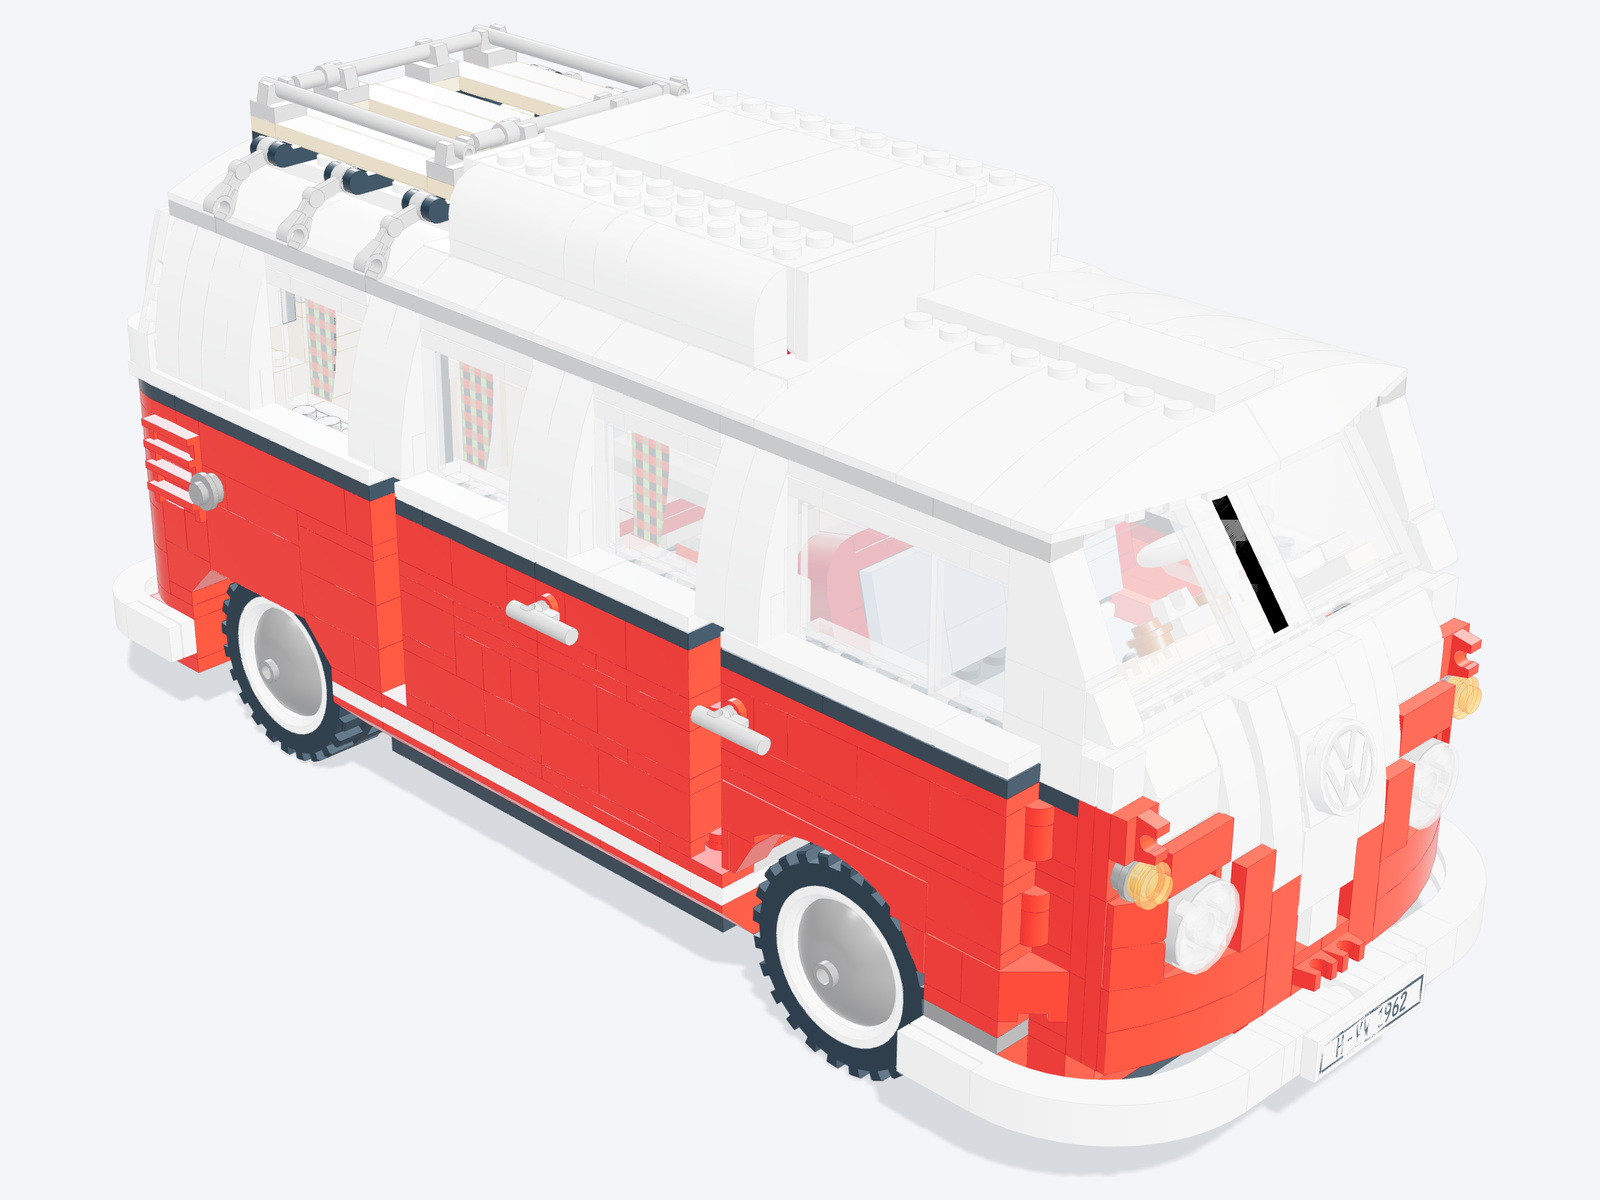
\includegraphics[width=.65\linewidth]{figures-v2/10220-iso.jpg}\end{center}
\paragraph{Attribution.}Stan Isachenko [angmarec]. CC BY 2.0.\par\url{https://library.ldraw.org/omr/sets/1294}
\paragraph{Source SHA256.}\path{ded9a68fc1b569e2965aa67febd225ab9d4b496a5d944247488d64c5d1619373}
\paragraph{Connector records.}stud: 3438; axle: 142; hinge: 23; fixed: 16; ball: 0
\paragraph{Public input lock.}\path{2068e99d6cb011f7c63a5b633d1a7f10b20f87b836e39c304ac89a84092e5159}
\paragraph{Status.}Source preservation does not certify stability. Reference outputs below are internal review material. Full model inputs are the versioned public JSON and numbered PNGs.
\begin{enumerate}
\item \textbf{ld2-10220-color-1}. Identify the original color of B0614; numbered isolation is allowed.
\par{\small color; visual; atomic; single-choice.\par\textit{Operands:} B0614 = brick\_000614\par\textit{Public evidence summary:} Numbered PNG: benchmark/ldraw-v2/inputs/views/ld2-10220-color-1.png; structured input = \{\}.\par\textit{Options:} A: Reddish Brown; B: White; C: Pearl Gold; D: Dark Red\par\textit{Reference output:} \{"choiceId": "A"\}\par\textit{Derivation:} source colorName by rendered B-label; source oracle only\par\textit{Equivalence:} exact declared response\par\textit{Review:} pending required human review.}
\item \textbf{ld2-10220-distance-1}. Using the supplied geometry bounding-box centers, which candidate is nearest to B0614?
\par{\small distance; source-data; atomic; single-choice.\par\textit{Operands:} B0977 = brick\_000977, B1232 = brick\_001232, B0847 = brick\_000847, B0614 = brick\_000614\par\textit{Public evidence summary:} \{"coordinateFrame": "Viewer world, millimeters, Euclidean distance", "centers": \{"B0614": [-24, 53.6, 24], "B0847": [48, 63.2, 216], "B1232": [32, 118.4, 152], "B0977": [36, 76, 128]\}\}\par\textit{Options:} A: B0977; B: B0847; C: B1232\par\textit{Reference output:} \{"choiceId": "A"\}\par\textit{Derivation:} Euclidean norm from public rounded centers\par\textit{Equivalence:} exact declared response\par\textit{Review:} machine checks passed; no human certification.}
\item \textbf{ld2-10220-color-2}. Identify the original color of B1293; numbered isolation is allowed.
\par{\small color; visual; atomic; single-choice.\par\textit{Operands:} B1293 = brick\_001293\par\textit{Public evidence summary:} Numbered PNG: benchmark/ldraw-v2/inputs/views/ld2-10220-color-2.png; structured input = \{\}.\par\textit{Options:} A: Bright Light Orange; B: Trans Clear; C: Light Bluish Grey; D: White\par\textit{Reference output:} \{"choiceId": "C"\}\par\textit{Derivation:} source colorName by rendered B-label; source oracle only\par\textit{Equivalence:} exact declared response\par\textit{Review:} pending required human review.}
\item \textbf{ld2-10220-shape-match-1}. Ignoring color and pose, which numbered instance has the same LDraw part type as B1293?
\par{\small shape-match; visual; atomic; single-choice.\par\textit{Operands:} B1423 = brick\_001423, B0952 = brick\_000952, B1293 = brick\_001293, B1161 = brick\_001161, B0657 = brick\_000657\par\textit{Public evidence summary:} Numbered PNG: benchmark/ldraw-v2/inputs/views/ld2-10220-shape-match-1.png; structured input = \{\}.\par\textit{Options:} A: B0952; B: B1161; C: B0657; D: B1423\par\textit{Reference output:} \{"choiceId": "B"\}\par\textit{Derivation:} source partNumber equality across labeled candidates; source oracle only\par\textit{Equivalence:} same source partNumber; ignore color and pose; perceptual equivalence pending\par\textit{Review:} pending required human review.}
\item \textbf{ld2-10220-distance-2}. Using the supplied geometry bounding-box centers, which candidate is nearest to B1293?
\par{\small distance; source-data; atomic; single-choice.\par\textit{Operands:} B1293 = brick\_001293, B1263 = brick\_001263, B0550 = brick\_000550, B0572 = brick\_000572\par\textit{Public evidence summary:} \{"coordinateFrame": "Viewer world, millimeters, Euclidean distance", "centers": \{"B1293": [-12, 122, 76], "B1263": [0, 114.4, 76], "B0550": [-52, 65.6, 156], "B0572": [0, 18.4, 244]\}\}\par\textit{Options:} A: B0550; B: B0572; C: B1263\par\textit{Reference output:} \{"choiceId": "C"\}\par\textit{Derivation:} Euclidean norm from public rounded centers\par\textit{Equivalence:} exact declared response\par\textit{Review:} machine checks passed; no human certification.}
\item \textbf{ld2-10220-color-3}. Identify the original color of B0285; numbered isolation is allowed.
\par{\small color; visual; atomic; single-choice.\par\textit{Operands:} B0285 = brick\_000285\par\textit{Public evidence summary:} Numbered PNG: benchmark/ldraw-v2/inputs/views/ld2-10220-color-3.png; structured input = \{\}.\par\textit{Options:} A: Trans Green; B: Light Bluish Grey; C: Yellow; D: Red\par\textit{Reference output:} \{"choiceId": "D"\}\par\textit{Derivation:} source colorName by rendered B-label; source oracle only\par\textit{Equivalence:} exact declared response\par\textit{Review:} pending required human review.}
\item \textbf{ld2-10220-shape-match-2}. Ignoring color and pose, which numbered instance has the same LDraw part type as B0285?
\par{\small shape-match; visual; atomic; single-choice.\par\textit{Operands:} B0780 = brick\_000780, B0415 = brick\_000415, B0874 = brick\_000874, B0479 = brick\_000479, B0285 = brick\_000285\par\textit{Public evidence summary:} Numbered PNG: benchmark/ldraw-v2/inputs/views/ld2-10220-shape-match-2.png; structured input = \{\}.\par\textit{Options:} A: B0415; B: B0479; C: B0780; D: B0874\par\textit{Reference output:} \{"choiceId": "C"\}\par\textit{Derivation:} source partNumber equality across labeled candidates; source oracle only\par\textit{Equivalence:} same source partNumber; ignore color and pose; perceptual equivalence pending\par\textit{Review:} pending required human review.}
\item \textbf{ld2-10220-distance-3}. Using the supplied geometry bounding-box centers, which candidate is nearest to B0285?
\par{\small distance; source-data; atomic; single-choice.\par\textit{Operands:} B0285 = brick\_000285, B0284 = brick\_000284, B0625 = brick\_000625, B0043 = brick\_000043\par\textit{Public evidence summary:} \{"coordinateFrame": "Viewer world, millimeters, Euclidean distance", "centers": \{"B0285": [-36, 2.4, 244], "B0284": [36, 2.4, 244], "B0043": [25.2, 15.2, 12], "B0625": [8, 45.6, 80.4]\}\}\par\textit{Options:} A: B0625; B: B0043; C: B0284\par\textit{Reference output:} \{"choiceId": "C"\}\par\textit{Derivation:} Euclidean norm from public rounded centers\par\textit{Equivalence:} exact declared response\par\textit{Review:} machine checks passed; no human certification.}
\item \textbf{ld2-10220-color-4}. Identify the original color of B0231; numbered isolation is allowed.
\par{\small color; visual; atomic; single-choice.\par\textit{Operands:} B0231 = brick\_000231\par\textit{Public evidence summary:} Numbered PNG: benchmark/ldraw-v2/inputs/views/ld2-10220-color-4.png; structured input = \{\}.\par\textit{Options:} A: Red; B: Dark Tan; C: Reddish Brown; D: Bright Light Orange\par\textit{Reference output:} \{"choiceId": "A"\}\par\textit{Derivation:} source colorName by rendered B-label; source oracle only\par\textit{Equivalence:} exact declared response\par\textit{Review:} pending required human review.}
\item \textbf{ld2-10220-shape-match-3}. Ignoring color and pose, which numbered instance has the same LDraw part type as B0231?
\par{\small shape-match; visual; atomic; single-choice.\par\textit{Operands:} B0743 = brick\_000743, B0231 = brick\_000231, B0485 = brick\_000485, B0255 = brick\_000255, B0747 = brick\_000747\par\textit{Public evidence summary:} Numbered PNG: benchmark/ldraw-v2/inputs/views/ld2-10220-shape-match-3.png; structured input = \{\}.\par\textit{Options:} A: B0255; B: B0485; C: B0747; D: B0743\par\textit{Reference output:} \{"choiceId": "A"\}\par\textit{Derivation:} source partNumber equality across labeled candidates; source oracle only\par\textit{Equivalence:} same source partNumber; ignore color and pose; perceptual equivalence pending\par\textit{Review:} pending required human review.}
\item \textbf{ld2-10220-distance-4}. Using the supplied geometry bounding-box centers, which candidate is nearest to B0231?
\par{\small distance; source-data; atomic; single-choice.\par\textit{Operands:} B1148 = brick\_001148, B0231 = brick\_000231, B0875 = brick\_000875, B0889 = brick\_000889\par\textit{Public evidence summary:} \{"coordinateFrame": "Viewer world, millimeters, Euclidean distance", "centers": \{"B0231": [-28, 2.4, 120], "B0875": [-32, 72.8, 85.4], "B0889": [-20, 95.2, 68], "B1148": [0, 113.6, 192]\}\}\par\textit{Options:} A: B1148; B: B0889; C: B0875\par\textit{Reference output:} \{"choiceId": "C"\}\par\textit{Derivation:} Euclidean norm from public rounded centers\par\textit{Equivalence:} exact declared response\par\textit{Review:} pending required human review.}
\item \textbf{ld2-10220-color-5}. Identify the original color of B0135; numbered isolation is allowed.
\par{\small color; visual; atomic; single-choice.\par\textit{Operands:} B0135 = brick\_000135\par\textit{Public evidence summary:} Numbered PNG: benchmark/ldraw-v2/inputs/views/ld2-10220-color-5.png; structured input = \{\}.\par\textit{Options:} A: Trans Red; B: Tan; C: Light Bluish Grey; D: Yellow\par\textit{Reference output:} \{"choiceId": "C"\}\par\textit{Derivation:} source colorName by rendered B-label; source oracle only\par\textit{Equivalence:} exact declared response\par\textit{Review:} pending required human review.}
\item \textbf{ld2-10220-shape-match-4}. Ignoring color and pose, which numbered instance has the same LDraw part type as B0135?
\par{\small shape-match; visual; atomic; single-choice.\par\textit{Operands:} B0439 = brick\_000439, B0411 = brick\_000411, B0501 = brick\_000501, B0702 = brick\_000702, B0135 = brick\_000135\par\textit{Public evidence summary:} Numbered PNG: benchmark/ldraw-v2/inputs/views/ld2-10220-shape-match-4.png; structured input = \{\}.\par\textit{Options:} A: B0439; B: B0702; C: B0411; D: B0501\par\textit{Reference output:} \{"choiceId": "D"\}\par\textit{Derivation:} source partNumber equality across labeled candidates; source oracle only\par\textit{Equivalence:} same source partNumber; ignore color and pose; perceptual equivalence pending\par\textit{Review:} pending required human review.}
\item \textbf{ld2-10220-distance-5}. Using the supplied geometry bounding-box centers, which candidate is nearest to B0135?
\par{\small distance; source-data; atomic; single-choice.\par\textit{Operands:} B0377 = brick\_000377, B0135 = brick\_000135, B0460 = brick\_000460, B0543 = brick\_000543\par\textit{Public evidence summary:} \{"coordinateFrame": "Viewer world, millimeters, Euclidean distance", "centers": \{"B0135": [20, 21.6, 44], "B0543": [-58.4, 56.8, 136], "B0377": [-36, 40.8, 4], "B0460": [-36, 31.2, 84]\}\}\par\textit{Options:} A: B0460; B: B0543; C: B0377\par\textit{Reference output:} \{"choiceId": "A"\}\par\textit{Derivation:} Euclidean norm from public rounded centers\par\textit{Equivalence:} exact declared response\par\textit{Review:} machine checks passed; no human certification.}
\item \textbf{ld2-10220-interface-1}. Classify the supplied connector record for B1302 and B1270. This does not certify load capacity.
\par{\small interface; connector-graph; metacognitive; single-choice.\par\textit{Operands:} B1302 = brick\_001302, B1270 = brick\_001270\par\textit{Public evidence summary:} \{"connectorRecord": \{"family": "axle", "aConnector": 1, "bConnector": 0\}, "scope": "Upstream connector tolerances and inset mesh intersections; unknown parts remain explicit, separate scene objects are not glued together; no load/force validation."\}\par\textit{Options:} A: hinge; B: axle; C: stud; D: ball; E: fixed\par\textit{Reference output:} \{"choiceId": "B"\}\par\textit{Derivation:} public connectorRecord.family equality\par\textit{Equivalence:} exact declared response\par\textit{Review:} machine checks passed; no human certification.}
\item \textbf{ld2-10220-interface-2}. Classify the supplied connector record for B1400 and B1404. This does not certify load capacity.
\par{\small interface; connector-graph; metacognitive; single-choice.\par\textit{Operands:} B1400 = brick\_001400, B1404 = brick\_001404\par\textit{Public evidence summary:} \{"connectorRecord": \{"family": "fixed", "aConnector": 1, "bConnector": 0\}, "scope": "Upstream connector tolerances and inset mesh intersections; unknown parts remain explicit, separate scene objects are not glued together; no load/force validation."\}\par\textit{Options:} A: fixed; B: hinge; C: ball; D: stud; E: axle\par\textit{Reference output:} \{"choiceId": "A"\}\par\textit{Derivation:} public connectorRecord.family equality\par\textit{Equivalence:} exact declared response\par\textit{Review:} machine checks passed; no human certification.}
\item \textbf{ld2-10220-interface-3}. Classify the supplied connector record for B0492 and B0491. This does not certify load capacity.
\par{\small interface; connector-graph; metacognitive; single-choice.\par\textit{Operands:} B0491 = brick\_000491, B0492 = brick\_000492\par\textit{Public evidence summary:} \{"connectorRecord": \{"family": "hinge", "aConnector": 1, "bConnector": 2\}, "scope": "Upstream connector tolerances and inset mesh intersections; unknown parts remain explicit, separate scene objects are not glued together; no load/force validation."\}\par\textit{Options:} A: fixed; B: axle; C: ball; D: stud; E: hinge\par\textit{Reference output:} \{"choiceId": "E"\}\par\textit{Derivation:} public connectorRecord.family equality\par\textit{Equivalence:} exact declared response\par\textit{Review:} machine checks passed; no human certification.}
\item \textbf{ld2-10220-interface-4}. Classify the supplied connector record for B0529 and B0542. This does not certify load capacity.
\par{\small interface; connector-graph; metacognitive; single-choice.\par\textit{Operands:} B0542 = brick\_000542, B0529 = brick\_000529\par\textit{Public evidence summary:} \{"connectorRecord": \{"family": "stud", "aConnector": 4, "bConnector": 0\}, "scope": "Upstream connector tolerances and inset mesh intersections; unknown parts remain explicit, separate scene objects are not glued together; no load/force validation."\}\par\textit{Options:} A: stud; B: hinge; C: fixed; D: ball; E: axle\par\textit{Reference output:} \{"choiceId": "A"\}\par\textit{Derivation:} public connectorRecord.family equality\par\textit{Equivalence:} exact declared response\par\textit{Review:} machine checks passed; no human certification.}
\item \textbf{ld2-10220-neighbors-1}. Select every candidate directly adjacent to B1336 in the supplied connector graph.
\par{\small neighbors; connector-graph; metacognitive; multiple-choice.\par\textit{Operands:} B1338 = brick\_001338, B1337 = brick\_001337, B0669 = brick\_000669, B0824 = brick\_000824, B1339 = brick\_001339, B1336 = brick\_001336\par\textit{Public evidence summary:} 3 unique undirected pairs\par\textit{Options:} A: B1337; B: B0669; C: B0824; D: B1338; E: B1339\par\textit{Reference output:} \{"choiceIds": ["A", "D", "E"]\}\par\textit{Derivation:} public incident edge endpoint set\par\textit{Equivalence:} unordered exact set; duplicate IDs invalid\par\textit{Review:} machine checks passed; no human certification.}
\item \textbf{ld2-10220-graph-removal-1}. Delete B1336 and its incident edges from this local graph. How many connected components remain? Do not infer physical extractability.
\par{\small graph-removal; connector-graph; graph-internal; integer.\par\textit{Operands:} B0824 = brick\_000824, B1339 = brick\_001339, B0669 = brick\_000669, B1338 = brick\_001338, B1337 = brick\_001337, B1336 = brick\_001336\par\textit{Public evidence summary:} 3 unique undirected pairs; 6 nodes\par\textit{Reference output:} \{"value": 5\}\par\textit{Derivation:} union-find component count after public target deletion\par\textit{Equivalence:} exact declared response\par\textit{Review:} machine checks passed; no human certification.}
\item \textbf{ld2-10220-neighbors-2}. Select every candidate directly adjacent to B0616 in the supplied connector graph.
\par{\small neighbors; connector-graph; metacognitive; multiple-choice.\par\textit{Operands:} B0601 = brick\_000601, B0120 = brick\_000120, B0871 = brick\_000871, B0616 = brick\_000616, B0501 = brick\_000501\par\textit{Public evidence summary:} 2 unique undirected pairs\par\textit{Options:} A: B0120; B: B0871; C: B0501; D: B0601\par\textit{Reference output:} \{"choiceIds": ["B", "D"]\}\par\textit{Derivation:} public incident edge endpoint set\par\textit{Equivalence:} unordered exact set; duplicate IDs invalid\par\textit{Review:} pending required human review.}
\item \textbf{ld2-10220-graph-removal-2}. Delete B0616 and its incident edges from this local graph. How many connected components remain? Do not infer physical extractability.
\par{\small graph-removal; connector-graph; graph-internal; integer.\par\textit{Operands:} B0501 = brick\_000501, B0871 = brick\_000871, B0601 = brick\_000601, B0120 = brick\_000120, B0616 = brick\_000616\par\textit{Public evidence summary:} 2 unique undirected pairs; 5 nodes\par\textit{Reference output:} \{"value": 4\}\par\textit{Derivation:} union-find component count after public target deletion\par\textit{Equivalence:} exact declared response\par\textit{Review:} pending required human review.}
\item \textbf{ld2-10220-neighbors-3}. Select every candidate directly adjacent to B0563 in the supplied connector graph.
\par{\small neighbors; connector-graph; metacognitive; multiple-choice.\par\textit{Operands:} B0563 = brick\_000563, B0312 = brick\_000312, B0643 = brick\_000643, B0116 = brick\_000116, B0566 = brick\_000566\par\textit{Public evidence summary:} 2 unique undirected pairs\par\textit{Options:} A: B0312; B: B0116; C: B0643; D: B0566\par\textit{Reference output:} \{"choiceIds": ["A", "D"]\}\par\textit{Derivation:} public incident edge endpoint set\par\textit{Equivalence:} unordered exact set; duplicate IDs invalid\par\textit{Review:} pending required human review.}
\item \textbf{ld2-10220-graph-removal-3}. Delete B0563 and its incident edges from this local graph. How many connected components remain? Do not infer physical extractability.
\par{\small graph-removal; connector-graph; graph-internal; integer.\par\textit{Operands:} B0563 = brick\_000563, B0312 = brick\_000312, B0116 = brick\_000116, B0643 = brick\_000643, B0566 = brick\_000566\par\textit{Public evidence summary:} 2 unique undirected pairs; 5 nodes\par\textit{Reference output:} \{"value": 4\}\par\textit{Derivation:} union-find component count after public target deletion\par\textit{Equivalence:} exact declared response\par\textit{Review:} pending required human review.}
\item \textbf{ld2-10220-neighbors-4}. Select every candidate directly adjacent to B0211 in the supplied connector graph.
\par{\small neighbors; connector-graph; metacognitive; multiple-choice.\par\textit{Operands:} B0208 = brick\_000208, B0211 = brick\_000211, B0365 = brick\_000365, B0213 = brick\_000213, B1378 = brick\_001378\par\textit{Public evidence summary:} 2 unique undirected pairs\par\textit{Options:} A: B1378; B: B0365; C: B0208; D: B0213\par\textit{Reference output:} \{"choiceIds": ["C", "D"]\}\par\textit{Derivation:} public incident edge endpoint set\par\textit{Equivalence:} unordered exact set; duplicate IDs invalid\par\textit{Review:} machine checks passed; no human certification.}
\item \textbf{ld2-10220-graph-removal-4}. Delete B0211 and its incident edges from this local graph. How many connected components remain? Do not infer physical extractability.
\par{\small graph-removal; connector-graph; graph-internal; integer.\par\textit{Operands:} B0211 = brick\_000211, B0208 = brick\_000208, B0213 = brick\_000213, B0365 = brick\_000365, B1378 = brick\_001378\par\textit{Public evidence summary:} 2 unique undirected pairs; 5 nodes\par\textit{Reference output:} \{"value": 4\}\par\textit{Derivation:} union-find component count after public target deletion\par\textit{Equivalence:} exact declared response\par\textit{Review:} machine checks passed; no human certification.}
\item \textbf{ld2-10220-neighbors-5}. Select every candidate directly adjacent to B0347 in the supplied connector graph.
\par{\small neighbors; connector-graph; metacognitive; multiple-choice.\par\textit{Operands:} B0338 = brick\_000338, B0368 = brick\_000368, B0347 = brick\_000347, B0356 = brick\_000356, B0344 = brick\_000344, B0357 = brick\_000357\par\textit{Public evidence summary:} 3 unique undirected pairs\par\textit{Options:} A: B0357; B: B0356; C: B0338; D: B0368; E: B0344\par\textit{Reference output:} \{"choiceIds": ["B", "C", "D"]\}\par\textit{Derivation:} public incident edge endpoint set\par\textit{Equivalence:} unordered exact set; duplicate IDs invalid\par\textit{Review:} machine checks passed; no human certification.}
\item \textbf{ld2-10220-graph-removal-5}. Delete B0347 and its incident edges from this local graph. How many connected components remain? Do not infer physical extractability.
\par{\small graph-removal; connector-graph; graph-internal; integer.\par\textit{Operands:} B0338 = brick\_000338, B0357 = brick\_000357, B0347 = brick\_000347, B0344 = brick\_000344, B0368 = brick\_000368, B0356 = brick\_000356\par\textit{Public evidence summary:} 3 unique undirected pairs; 6 nodes\par\textit{Reference output:} \{"value": 5\}\par\textit{Derivation:} union-find component count after public target deletion\par\textit{Equivalence:} exact declared response\par\textit{Review:} machine checks passed; no human certification.}
\item \textbf{ld2-10220-coverage-1}. Which numbered instance lacks a connector definition in the coverage record, so this audit cannot establish that it is floating?
\par{\small coverage; source-data; metacognitive; single-choice.\par\textit{Operands:} B0285 = brick\_000285, B0045 = brick\_000045, B1293 = brick\_001293, B0614 = brick\_000614\par\textit{Public evidence summary:} \{"coverage": [\{"label": "B0285", "supported": true\}, \{"label": "B0614", "supported": true\}, \{"label": "B1293", "supported": true\}, \{"label": "B0045", "supported": false\}]\}\par\textit{Options:} A: B0045; B: B1293; C: B0285; D: B0614\par\textit{Reference output:} \{"choiceId": "A"\}\par\textit{Derivation:} public supported=false record\par\textit{Equivalence:} exact declared response\par\textit{Review:} pending required human review.}
\item \textbf{ld2-10220-evidence-limit-1}. Only source geometry, connector matching and mesh intersection audits are available. Without mass, friction, material or dynamic tests, is gravitational stability established?
\par{\small evidence-limit; source-data; metacognitive; single-choice.\par\textit{Operands:} none\par\textit{Public evidence summary:} \{"available": ["Original CAD", "Connector inference", "Inset-mesh intersection candidates"]\}\par\textit{Options:} A: Not established by this evidence; B: Established\par\textit{Reference output:} \{"choiceId": "A"\}\par\textit{Derivation:} fixed epistemic control label\par\textit{Equivalence:} exact declared response\par\textit{Review:} machine checks passed; no human certification.}
\item \textbf{ld2-10220-source-step-1}. At which expanded author step does B0301 first appear in the supplied source-step table? Source order is not a collision-free assembly proof.
\par{\small source-step; source-data; procedural; single-choice.\par\textit{Operands:} B0001 = brick\_000001, B0301 = brick\_000301\par\textit{Public evidence summary:} 2 supplied author-step records; exact table in public JSON\par\textit{Options:} A: 2; B: 13; C: 300; D: 71\par\textit{Reference output:} \{"choiceId": "D"\}\par\textit{Derivation:} minimum public step index containing target\par\textit{Equivalence:} exact declared response\par\textit{Review:} machine checks passed; no human certification.}
\item \textbf{ld2-10220-source-step-2}. At which expanded author step does B1307 first appear in the supplied source-step table? Source order is not a collision-free assembly proof.
\par{\small source-step; source-data; procedural; single-choice.\par\textit{Operands:} B0001 = brick\_000001, B1307 = brick\_001307\par\textit{Public evidence summary:} 2 supplied author-step records; exact table in public JSON\par\textit{Options:} A: 122; B: 382; C: 234; D: 149\par\textit{Reference output:} \{"choiceId": "B"\}\par\textit{Derivation:} minimum public step index containing target\par\textit{Equivalence:} exact declared response\par\textit{Review:} machine checks passed; no human certification.}
\item \textbf{ld2-10220-source-step-3}. At which expanded author step does B1400 first appear in the supplied source-step table? Source order is not a collision-free assembly proof.
\par{\small source-step; source-data; procedural; single-choice.\par\textit{Operands:} B0001 = brick\_000001, B1400 = brick\_001400\par\textit{Public evidence summary:} 2 supplied author-step records; exact table in public JSON\par\textit{Options:} A: 418; B: 414; C: 423; D: 4\par\textit{Reference output:} \{"choiceId": "B"\}\par\textit{Derivation:} minimum public step index containing target\par\textit{Equivalence:} exact declared response\par\textit{Review:} machine checks passed; no human certification.}
\item \textbf{ld2-10220-source-step-4}. At which expanded author step does B0973 first appear in the supplied source-step table? Source order is not a collision-free assembly proof.
\par{\small source-step; source-data; procedural; single-choice.\par\textit{Operands:} B0001 = brick\_000001, B0973 = brick\_000973\par\textit{Public evidence summary:} 2 supplied author-step records; exact table in public JSON\par\textit{Options:} A: 153; B: 391; C: 266; D: 286\par\textit{Reference output:} \{"choiceId": "C"\}\par\textit{Derivation:} minimum public step index containing target\par\textit{Equivalence:} exact declared response\par\textit{Review:} machine checks passed; no human certification.}
\item \textbf{ld2-10220-source-step-5}. At which expanded author step does B1420 first appear in the supplied source-step table? Source order is not a collision-free assembly proof.
\par{\small source-step; source-data; procedural; single-choice.\par\textit{Operands:} B0001 = brick\_000001, B1420 = brick\_001420\par\textit{Public evidence summary:} 2 supplied author-step records; exact table in public JSON\par\textit{Options:} A: 43; B: 152; C: 430; D: 432\par\textit{Reference output:} \{"choiceId": "C"\}\par\textit{Derivation:} minimum public step index containing target\par\textit{Equivalence:} exact declared response\par\textit{Review:} machine checks passed; no human certification.}
\item \textbf{ld2-10220-source-sequence-1}. Reveal the supplied source-step window in author order. Actions change visibility only, without simulating insertion trajectories.
\par{\small source-sequence; scene-edit; procedural; actions.\par\textit{Operands:} B0016 = brick\_000016, B0012 = brick\_000012, B0022 = brick\_000022, B0011 = brick\_000011, B0001 = brick\_000001, B0009 = brick\_000009, B0007 = brick\_000007, B0008 = brick\_000008, B0002 = brick\_000002, B0006 = brick\_000006, B0017 = brick\_000017, B0010 = brick\_000010, B0023 = brick\_000023, B0003 = brick\_000003, B0015 = brick\_000015, B0020 = brick\_000020, B0005 = brick\_000005, B0004 = brick\_000004, B0018 = brick\_000018, B0021 = brick\_000021, B0013 = brick\_000013, B0014 = brick\_000014, B0019 = brick\_000019\par\textit{Public evidence summary:} 6 public actions; budget 6; \{"initialFacts": ["start"], "goalFacts": ["done-6"], "absentFacts": []\}\par\textit{Reference output:} \{"actionIds": ["step-1", "step-2", "step-3", "step-4", "step-5", "step-6"]\}\par\textit{Derivation:} public precondition solver\par\textit{Equivalence:} any legal sequence reaching all goals within budget; display-only semantics\par\textit{Review:} machine checks passed; no human certification.}
\item \textbf{ld2-10220-restore-instance-1}. The display copy hides B0614. Restore only that numbered instance, preserving all other instances and source poses.
\par{\small restore-instance; scene-edit; procedural; actions.\par\textit{Operands:} B0614 = brick\_000614, B0001 = brick\_000001\par\textit{Public evidence summary:} 2 public actions; budget 1; \{"initialFacts": ["missing-brick\_000614", "present-brick\_000001"], "goalFacts": ["present-brick\_000614", "present-brick\_000001"], "absentFacts": ["missing-brick\_000614"]\}\par\textit{Reference output:} \{"actionIds": ["restore-B0614"]\}\par\textit{Derivation:} public precondition solver\par\textit{Equivalence:} any legal sequence reaching all goals within budget; display-only semantics\par\textit{Review:} machine checks passed; no human certification.}
\item \textbf{ld2-10220-restore-instance-2}. The display copy hides B1293. Restore only that numbered instance, preserving all other instances and source poses.
\par{\small restore-instance; scene-edit; procedural; actions.\par\textit{Operands:} B0001 = brick\_000001, B1293 = brick\_001293\par\textit{Public evidence summary:} 2 public actions; budget 1; \{"initialFacts": ["missing-brick\_001293", "present-brick\_000001"], "goalFacts": ["present-brick\_001293", "present-brick\_000001"], "absentFacts": ["missing-brick\_001293"]\}\par\textit{Reference output:} \{"actionIds": ["restore-B1293"]\}\par\textit{Derivation:} public precondition solver\par\textit{Equivalence:} any legal sequence reaching all goals within budget; display-only semantics\par\textit{Review:} machine checks passed; no human certification.}
\item \textbf{ld2-10220-restore-instance-3}. The display copy hides B0285. Restore only that numbered instance, preserving all other instances and source poses.
\par{\small restore-instance; scene-edit; procedural; actions.\par\textit{Operands:} B0285 = brick\_000285, B0001 = brick\_000001\par\textit{Public evidence summary:} 2 public actions; budget 1; \{"initialFacts": ["missing-brick\_000285", "present-brick\_000001"], "goalFacts": ["present-brick\_000285", "present-brick\_000001"], "absentFacts": ["missing-brick\_000285"]\}\par\textit{Reference output:} \{"actionIds": ["restore-B0285"]\}\par\textit{Derivation:} public precondition solver\par\textit{Equivalence:} any legal sequence reaching all goals within budget; display-only semantics\par\textit{Review:} machine checks passed; no human certification.}
\end{enumerate}
\clearpage\section{21309: NASA Apollo Saturn V}
1845 source instances; 39 tasks; D4 size band. 141 type strings; 14 color codes; 0 unsupported instances; 67 intersection candidates. 940 expanded author steps. Independent reparse: passed.
\begin{center}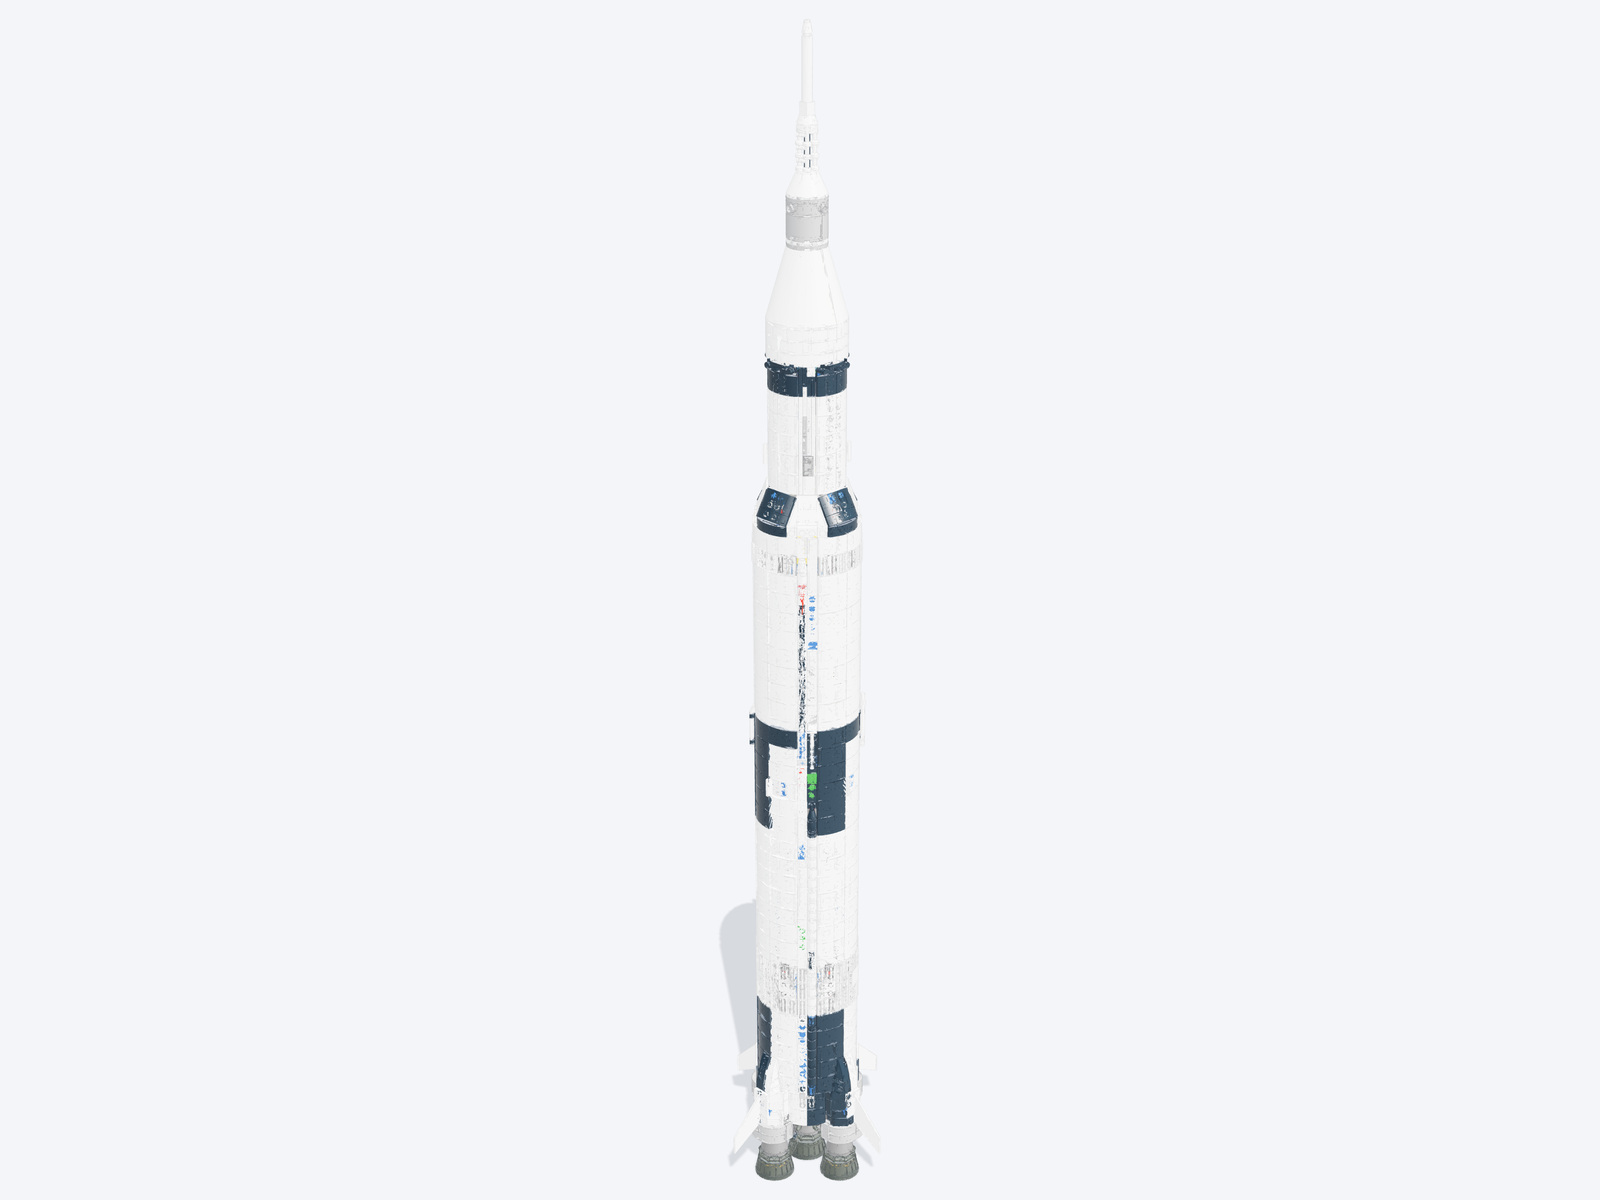
\includegraphics[width=.65\linewidth]{figures-v2/omr-21309-iso.jpg}\end{center}
\paragraph{Attribution.}Jaco van der Molen [Jaco]. CC BY 2.0.\par\url{https://library.ldraw.org/library/omr/21309-1.mpd}
\paragraph{Source SHA256.}\path{eb56995265201179e0ecbad2865fb62fced524c44f3a4179badc964f844e5ba1}
\paragraph{Connector records.}stud: 5100; axle: 216; hinge: 16; fixed: 0; ball: 8
\paragraph{Public input lock.}\path{ae3142670b3b9f1b513a31473a59d676926e2f17657b32026a5d28cbe49e947b}
\paragraph{Status.}Source preservation does not certify stability. Reference outputs below are internal review material. Full model inputs are the versioned public JSON and numbered PNGs.
\begin{enumerate}
\item \textbf{ld2-omr-21309-color-1}. Identify the original color of B0496; numbered isolation is allowed.
\par{\small color; visual; atomic; single-choice.\par\textit{Operands:} B0496 = brick\_000496\par\textit{Public evidence summary:} Numbered PNG: benchmark/ldraw-v2/inputs/views/ld2-omr-21309-color-1.png; structured input = \{\}.\par\textit{Options:} A: Pearl Light Grey; B: White; C: Trans Orange; D: Yellow\par\textit{Reference output:} \{"choiceId": "B"\}\par\textit{Derivation:} source colorName by rendered B-label; source oracle only\par\textit{Equivalence:} exact declared response\par\textit{Review:} pending required human review.}
\item \textbf{ld2-omr-21309-shape-match-1}. Ignoring color and pose, which numbered instance has the same LDraw part type as B0496?
\par{\small shape-match; visual; atomic; single-choice.\par\textit{Operands:} B0496 = brick\_000496, B1676 = brick\_001676, B0498 = brick\_000498, B0171 = brick\_000171, B1478 = brick\_001478\par\textit{Public evidence summary:} Numbered PNG: benchmark/ldraw-v2/inputs/views/ld2-omr-21309-shape-match-1.png; structured input = \{\}.\par\textit{Options:} A: B1676; B: B0171; C: B0498; D: B1478\par\textit{Reference output:} \{"choiceId": "C"\}\par\textit{Derivation:} source partNumber equality across labeled candidates; source oracle only\par\textit{Equivalence:} same source partNumber; ignore color and pose; perceptual equivalence pending\par\textit{Review:} pending required human review.}
\item \textbf{ld2-omr-21309-distance-1}. Using the supplied geometry bounding-box centers, which candidate is nearest to B0496?
\par{\small distance; source-data; atomic; single-choice.\par\textit{Operands:} B1211 = brick\_001211, B1130 = brick\_001130, B0496 = brick\_000496, B0093 = brick\_000093\par\textit{Public evidence summary:} \{"coordinateFrame": "Viewer world, millimeters, Euclidean distance", "centers": \{"B0496": [-32.5858, 222.4, 26.9286], "B1211": [-33.01, 454.4, 27.354], "B1130": [-20, 532, 0], "B0093": [4, 122.4, -16.4]\}\}\par\textit{Options:} A: B1130; B: B0093; C: B1211\par\textit{Reference output:} \{"choiceId": "B"\}\par\textit{Derivation:} Euclidean norm from public rounded centers\par\textit{Equivalence:} exact declared response\par\textit{Review:} machine checks passed; no human certification.}
\item \textbf{ld2-omr-21309-color-2}. Identify the original color of B0439; numbered isolation is allowed.
\par{\small color; visual; atomic; single-choice.\par\textit{Operands:} B0439 = brick\_000439\par\textit{Public evidence summary:} Numbered PNG: benchmark/ldraw-v2/inputs/views/ld2-omr-21309-color-2.png; structured input = \{\}.\par\textit{Options:} A: Blue; B: Red; C: White; D: Dark Bluish Grey\par\textit{Reference output:} \{"choiceId": "B"\}\par\textit{Derivation:} source colorName by rendered B-label; source oracle only\par\textit{Equivalence:} exact declared response\par\textit{Review:} pending required human review.}
\item \textbf{ld2-omr-21309-shape-match-2}. Ignoring color and pose, which numbered instance has the same LDraw part type as B0439?
\par{\small shape-match; visual; atomic; single-choice.\par\textit{Operands:} B0454 = brick\_000454, B0536 = brick\_000536, B0843 = brick\_000843, B0439 = brick\_000439, B1793 = brick\_001793\par\textit{Public evidence summary:} Numbered PNG: benchmark/ldraw-v2/inputs/views/ld2-omr-21309-shape-match-2.png; structured input = \{\}.\par\textit{Options:} A: B1793; B: B0843; C: B0454; D: B0536\par\textit{Reference output:} \{"choiceId": "C"\}\par\textit{Derivation:} source partNumber equality across labeled candidates; source oracle only\par\textit{Equivalence:} same source partNumber; ignore color and pose; perceptual equivalence pending\par\textit{Review:} pending required human review.}
\item \textbf{ld2-omr-21309-distance-2}. Using the supplied geometry bounding-box centers, which candidate is nearest to B0439?
\par{\small distance; source-data; atomic; single-choice.\par\textit{Operands:} B0642 = brick\_000642, B0439 = brick\_000439, B1371 = brick\_001371, B0194 = brick\_000194\par\textit{Public evidence summary:} \{"coordinateFrame": "Viewer world, millimeters, Euclidean distance", "centers": \{"B0439": [22.2624, 329.20596, 27.9184], "B0194": [40, 154.4, 12], "B0642": [-20.4486, 142.4, -38.3838], "B1371": [-40, 366.4, 12]\}\}\par\textit{Options:} A: B0642; B: B0194; C: B1371\par\textit{Reference output:} \{"choiceId": "C"\}\par\textit{Derivation:} Euclidean norm from public rounded centers\par\textit{Equivalence:} exact declared response\par\textit{Review:} machine checks passed; no human certification.}
\item \textbf{ld2-omr-21309-color-3}. Identify the original color of B1134; numbered isolation is allowed.
\par{\small color; visual; atomic; single-choice.\par\textit{Operands:} B1134 = brick\_001134\par\textit{Public evidence summary:} Numbered PNG: benchmark/ldraw-v2/inputs/views/ld2-omr-21309-color-3.png; structured input = \{\}.\par\textit{Options:} A: Black; B: Yellow; C: Trans Orange; D: Green\par\textit{Reference output:} \{"choiceId": "A"\}\par\textit{Derivation:} source colorName by rendered B-label; source oracle only\par\textit{Equivalence:} exact declared response\par\textit{Review:} pending required human review.}
\item \textbf{ld2-omr-21309-shape-match-3}. Ignoring color and pose, which numbered instance has the same LDraw part type as B1134?
\par{\small shape-match; visual; atomic; single-choice.\par\textit{Operands:} B1633 = brick\_001633, B1136 = brick\_001136, B0274 = brick\_000274, B0809 = brick\_000809, B1134 = brick\_001134\par\textit{Public evidence summary:} Numbered PNG: benchmark/ldraw-v2/inputs/views/ld2-omr-21309-shape-match-3.png; structured input = \{\}.\par\textit{Options:} A: B1633; B: B1136; C: B0809; D: B0274\par\textit{Reference output:} \{"choiceId": "B"\}\par\textit{Derivation:} source partNumber equality across labeled candidates; source oracle only\par\textit{Equivalence:} same source partNumber; ignore color and pose; perceptual equivalence pending\par\textit{Review:} pending required human review.}
\item \textbf{ld2-omr-21309-distance-3}. Using the supplied geometry bounding-box centers, which candidate is nearest to B1134?
\par{\small distance; source-data; atomic; single-choice.\par\textit{Operands:} B1800 = brick\_001800, B1134 = brick\_001134, B1704 = brick\_001704, B1365 = brick\_001365\par\textit{Public evidence summary:} \{"coordinateFrame": "Viewer world, millimeters, Euclidean distance", "centers": \{"B1134": [-20, 538.4, 16.8], "B1365": [-34.4, 534.4, 0], "B1800": [0, 770.39994, 0], "B1704": [0, 570.4, 19.200032]\}\}\par\textit{Options:} A: B1365; B: B1704; C: B1800\par\textit{Reference output:} \{"choiceId": "A"\}\par\textit{Derivation:} Euclidean norm from public rounded centers\par\textit{Equivalence:} exact declared response\par\textit{Review:} machine checks passed; no human certification.}
\item \textbf{ld2-omr-21309-color-4}. Identify the original color of B0754; numbered isolation is allowed.
\par{\small color; visual; atomic; single-choice.\par\textit{Operands:} B0754 = brick\_000754\par\textit{Public evidence summary:} Numbered PNG: benchmark/ldraw-v2/inputs/views/ld2-omr-21309-color-4.png; structured input = \{\}.\par\textit{Options:} A: Pearl Gold; B: Black; C: Light Bluish Grey; D: Green\par\textit{Reference output:} \{"choiceId": "C"\}\par\textit{Derivation:} source colorName by rendered B-label; source oracle only\par\textit{Equivalence:} exact declared response\par\textit{Review:} pending required human review.}
\item \textbf{ld2-omr-21309-shape-match-4}. Ignoring color and pose, which numbered instance has the same LDraw part type as B0754?
\par{\small shape-match; visual; atomic; single-choice.\par\textit{Operands:} B0212 = brick\_000212, B0004 = brick\_000004, B0036 = brick\_000036, B0684 = brick\_000684, B0754 = brick\_000754\par\textit{Public evidence summary:} Numbered PNG: benchmark/ldraw-v2/inputs/views/ld2-omr-21309-shape-match-4.png; structured input = \{\}.\par\textit{Options:} A: B0036; B: B0212; C: B0004; D: B0684\par\textit{Reference output:} \{"choiceId": "D"\}\par\textit{Derivation:} source partNumber equality across labeled candidates; source oracle only\par\textit{Equivalence:} same source partNumber; ignore color and pose; perceptual equivalence pending\par\textit{Review:} pending required human review.}
\item \textbf{ld2-omr-21309-distance-4}. Using the supplied geometry bounding-box centers, which candidate is nearest to B0754?
\par{\small distance; source-data; atomic; single-choice.\par\textit{Operands:} B1554 = brick\_001554, B0068 = brick\_000068, B1390 = brick\_001390, B0754 = brick\_000754\par\textit{Public evidence summary:} \{"coordinateFrame": "Viewer world, millimeters, Euclidean distance", "centers": \{"B0754": [17.3568, 142.4, -33.8352], "B1390": [-40, 486.4, -12], "B0068": [27.3536, 54.4, 27.3536], "B1554": [8, 566.264406, -34.264011]\}\}\par\textit{Options:} A: B0068; B: B1390; C: B1554\par\textit{Reference output:} \{"choiceId": "A"\}\par\textit{Derivation:} Euclidean norm from public rounded centers\par\textit{Equivalence:} exact declared response\par\textit{Review:} pending required human review.}
\item \textbf{ld2-omr-21309-color-5}. Identify the original color of B1147; numbered isolation is allowed.
\par{\small color; visual; atomic; single-choice.\par\textit{Operands:} B1147 = brick\_001147\par\textit{Public evidence summary:} Numbered PNG: benchmark/ldraw-v2/inputs/views/ld2-omr-21309-color-5.png; structured input = \{\}.\par\textit{Options:} A: Black; B: Trans Orange; C: Red; D: Blue\par\textit{Reference output:} \{"choiceId": "D"\}\par\textit{Derivation:} source colorName by rendered B-label; source oracle only\par\textit{Equivalence:} exact declared response\par\textit{Review:} pending required human review.}
\item \textbf{ld2-omr-21309-shape-match-5}. Ignoring color and pose, which numbered instance has the same LDraw part type as B1147?
\par{\small shape-match; visual; atomic; single-choice.\par\textit{Operands:} B1175 = brick\_001175, B1740 = brick\_001740, B1154 = brick\_001154, B1410 = brick\_001410, B1147 = brick\_001147\par\textit{Public evidence summary:} Numbered PNG: benchmark/ldraw-v2/inputs/views/ld2-omr-21309-shape-match-5.png; structured input = \{\}.\par\textit{Options:} A: B1740; B: B1175; C: B1410; D: B1154\par\textit{Reference output:} \{"choiceId": "A"\}\par\textit{Derivation:} source partNumber equality across labeled candidates; source oracle only\par\textit{Equivalence:} same source partNumber; ignore color and pose; perceptual equivalence pending\par\textit{Review:} pending required human review.}
\item \textbf{ld2-omr-21309-distance-5}. Using the supplied geometry bounding-box centers, which candidate is nearest to B1147?
\par{\small distance; source-data; atomic; single-choice.\par\textit{Operands:} B1147 = brick\_001147, B0920 = brick\_000920, B1765 = brick\_001765, B1750 = brick\_001750\par\textit{Public evidence summary:} \{"coordinateFrame": "Viewer world, millimeters, Euclidean distance", "centers": \{"B1147": [0, 340, 12], "B1750": [17.7936, 602.4, -18.7872], "B0920": [-26.2216, 6.4, 26.2216], "B1765": [8, 646.4, 28.800012]\}\}\par\textit{Options:} A: B1750; B: B0920; C: B1765\par\textit{Reference output:} \{"choiceId": "A"\}\par\textit{Derivation:} Euclidean norm from public rounded centers\par\textit{Equivalence:} exact declared response\par\textit{Review:} machine checks passed; no human certification.}
\item \textbf{ld2-omr-21309-interface-1}. Classify the supplied connector record for B0478 and B0477. This does not certify load capacity.
\par{\small interface; connector-graph; metacognitive; single-choice.\par\textit{Operands:} B0478 = brick\_000478, B0477 = brick\_000477\par\textit{Public evidence summary:} \{"connectorRecord": \{"family": "axle", "aConnector": 1, "bConnector": 0\}, "scope": "Upstream connector tolerances and inset mesh intersections; unknown parts remain explicit, separate scene objects are not glued together; no load/force validation."\}\par\textit{Options:} A: axle; B: fixed; C: ball; D: stud; E: hinge\par\textit{Reference output:} \{"choiceId": "A"\}\par\textit{Derivation:} public connectorRecord.family equality\par\textit{Equivalence:} exact declared response\par\textit{Review:} machine checks passed; no human certification.}
\item \textbf{ld2-omr-21309-interface-2}. Classify the supplied connector record for B1615 and B1737. This does not certify load capacity.
\par{\small interface; connector-graph; metacognitive; single-choice.\par\textit{Operands:} B1737 = brick\_001737, B1615 = brick\_001615\par\textit{Public evidence summary:} \{"connectorRecord": \{"family": "ball", "aConnector": 3, "bConnector": 3\}, "scope": "Upstream connector tolerances and inset mesh intersections; unknown parts remain explicit, separate scene objects are not glued together; no load/force validation."\}\par\textit{Options:} A: axle; B: stud; C: fixed; D: ball; E: hinge\par\textit{Reference output:} \{"choiceId": "D"\}\par\textit{Derivation:} public connectorRecord.family equality\par\textit{Equivalence:} exact declared response\par\textit{Review:} machine checks passed; no human certification.}
\item \textbf{ld2-omr-21309-interface-3}. Classify the supplied connector record for B0204 and B0868. This does not certify load capacity.
\par{\small interface; connector-graph; metacognitive; single-choice.\par\textit{Operands:} B0204 = brick\_000204, B0868 = brick\_000868\par\textit{Public evidence summary:} \{"connectorRecord": \{"family": "hinge", "aConnector": 1, "bConnector": 1\}, "scope": "Upstream connector tolerances and inset mesh intersections; unknown parts remain explicit, separate scene objects are not glued together; no load/force validation."\}\par\textit{Options:} A: fixed; B: axle; C: ball; D: stud; E: hinge\par\textit{Reference output:} \{"choiceId": "E"\}\par\textit{Derivation:} public connectorRecord.family equality\par\textit{Equivalence:} exact declared response\par\textit{Review:} pending required human review.}
\item \textbf{ld2-omr-21309-interface-4}. Classify the supplied connector record for B0965 and B0967. This does not certify load capacity.
\par{\small interface; connector-graph; metacognitive; single-choice.\par\textit{Operands:} B0965 = brick\_000965, B0967 = brick\_000967\par\textit{Public evidence summary:} \{"connectorRecord": \{"family": "stud", "aConnector": 13, "bConnector": 3\}, "scope": "Upstream connector tolerances and inset mesh intersections; unknown parts remain explicit, separate scene objects are not glued together; no load/force validation."\}\par\textit{Options:} A: axle; B: hinge; C: stud; D: ball; E: fixed\par\textit{Reference output:} \{"choiceId": "C"\}\par\textit{Derivation:} public connectorRecord.family equality\par\textit{Equivalence:} exact declared response\par\textit{Review:} machine checks passed; no human certification.}
\item \textbf{ld2-omr-21309-neighbors-1}. Select every candidate directly adjacent to B1441 in the supplied connector graph.
\par{\small neighbors; connector-graph; metacognitive; multiple-choice.\par\textit{Operands:} B1435 = brick\_001435, B1441 = brick\_001441, B1549 = brick\_001549, B0432 = brick\_000432, B1437 = brick\_001437\par\textit{Public evidence summary:} 3 unique undirected pairs\par\textit{Options:} A: B0432; B: B1549; C: B1437; D: B1435\par\textit{Reference output:} \{"choiceIds": ["C", "D"]\}\par\textit{Derivation:} public incident edge endpoint set\par\textit{Equivalence:} unordered exact set; duplicate IDs invalid\par\textit{Review:} pending required human review.}
\item \textbf{ld2-omr-21309-graph-removal-1}. Delete B1441 and its incident edges from this local graph. How many connected components remain? Do not infer physical extractability.
\par{\small graph-removal; connector-graph; graph-internal; integer.\par\textit{Operands:} B1437 = brick\_001437, B1435 = brick\_001435, B1441 = brick\_001441, B1549 = brick\_001549, B0432 = brick\_000432\par\textit{Public evidence summary:} 3 unique undirected pairs; 5 nodes\par\textit{Reference output:} \{"value": 3\}\par\textit{Derivation:} union-find component count after public target deletion\par\textit{Equivalence:} exact declared response\par\textit{Review:} pending required human review.}
\item \textbf{ld2-omr-21309-neighbors-2}. Select every candidate directly adjacent to B1250 in the supplied connector graph.
\par{\small neighbors; connector-graph; metacognitive; multiple-choice.\par\textit{Operands:} B0989 = brick\_000989, B1251 = brick\_001251, B1250 = brick\_001250, B1231 = brick\_001231, B1019 = brick\_001019, B1252 = brick\_001252, B1253 = brick\_001253, B1831 = brick\_001831\par\textit{Public evidence summary:} 5 unique undirected pairs\par\textit{Options:} A: B0989; B: B1231; C: B1019; D: B1252; E: B1251; F: B1831; G: B1253\par\textit{Reference output:} \{"choiceIds": ["A", "C", "D", "E", "G"]\}\par\textit{Derivation:} public incident edge endpoint set\par\textit{Equivalence:} unordered exact set; duplicate IDs invalid\par\textit{Review:} machine checks passed; no human certification.}
\item \textbf{ld2-omr-21309-graph-removal-2}. Delete B1250 and its incident edges from this local graph. How many connected components remain? Do not infer physical extractability.
\par{\small graph-removal; connector-graph; graph-internal; integer.\par\textit{Operands:} B1231 = brick\_001231, B1831 = brick\_001831, B1251 = brick\_001251, B1019 = brick\_001019, B1252 = brick\_001252, B1253 = brick\_001253, B0989 = brick\_000989, B1250 = brick\_001250\par\textit{Public evidence summary:} 5 unique undirected pairs; 8 nodes\par\textit{Reference output:} \{"value": 7\}\par\textit{Derivation:} union-find component count after public target deletion\par\textit{Equivalence:} exact declared response\par\textit{Review:} machine checks passed; no human certification.}
\item \textbf{ld2-omr-21309-neighbors-3}. Select every candidate directly adjacent to B1039 in the supplied connector graph.
\par{\small neighbors; connector-graph; metacognitive; multiple-choice.\par\textit{Operands:} B0670 = brick\_000670, B1422 = brick\_001422, B1040 = brick\_001040, B1039 = brick\_001039, B1038 = brick\_001038\par\textit{Public evidence summary:} 2 unique undirected pairs\par\textit{Options:} A: B0670; B: B1422; C: B1040; D: B1038\par\textit{Reference output:} \{"choiceIds": ["C", "D"]\}\par\textit{Derivation:} public incident edge endpoint set\par\textit{Equivalence:} unordered exact set; duplicate IDs invalid\par\textit{Review:} machine checks passed; no human certification.}
\item \textbf{ld2-omr-21309-graph-removal-3}. Delete B1039 and its incident edges from this local graph. How many connected components remain? Do not infer physical extractability.
\par{\small graph-removal; connector-graph; graph-internal; integer.\par\textit{Operands:} B1039 = brick\_001039, B1038 = brick\_001038, B1422 = brick\_001422, B1040 = brick\_001040, B0670 = brick\_000670\par\textit{Public evidence summary:} 2 unique undirected pairs; 5 nodes\par\textit{Reference output:} \{"value": 4\}\par\textit{Derivation:} union-find component count after public target deletion\par\textit{Equivalence:} exact declared response\par\textit{Review:} machine checks passed; no human certification.}
\item \textbf{ld2-omr-21309-neighbors-4}. Select every candidate directly adjacent to B0435 in the supplied connector graph.
\par{\small neighbors; connector-graph; metacognitive; multiple-choice.\par\textit{Operands:} B0424 = brick\_000424, B0657 = brick\_000657, B0435 = brick\_000435, B0484 = brick\_000484, B0499 = brick\_000499, B0485 = brick\_000485, B0193 = brick\_000193\par\textit{Public evidence summary:} 4 unique undirected pairs\par\textit{Options:} A: B0424; B: B0657; C: B0499; D: B0485; E: B0484; F: B0193\par\textit{Reference output:} \{"choiceIds": ["A", "C", "D", "E"]\}\par\textit{Derivation:} public incident edge endpoint set\par\textit{Equivalence:} unordered exact set; duplicate IDs invalid\par\textit{Review:} machine checks passed; no human certification.}
\item \textbf{ld2-omr-21309-graph-removal-4}. Delete B0435 and its incident edges from this local graph. How many connected components remain? Do not infer physical extractability.
\par{\small graph-removal; connector-graph; graph-internal; integer.\par\textit{Operands:} B0193 = brick\_000193, B0435 = brick\_000435, B0485 = brick\_000485, B0484 = brick\_000484, B0657 = brick\_000657, B0499 = brick\_000499, B0424 = brick\_000424\par\textit{Public evidence summary:} 4 unique undirected pairs; 7 nodes\par\textit{Reference output:} \{"value": 6\}\par\textit{Derivation:} union-find component count after public target deletion\par\textit{Equivalence:} exact declared response\par\textit{Review:} machine checks passed; no human certification.}
\item \textbf{ld2-omr-21309-neighbors-5}. Select every candidate directly adjacent to B1053 in the supplied connector graph.
\par{\small neighbors; connector-graph; metacognitive; multiple-choice.\par\textit{Operands:} B0416 = brick\_000416, B1054 = brick\_001054, B0538 = brick\_000538, B1053 = brick\_001053, B1055 = brick\_001055\par\textit{Public evidence summary:} 2 unique undirected pairs\par\textit{Options:} A: B0416; B: B1055; C: B0538; D: B1054\par\textit{Reference output:} \{"choiceIds": ["B", "D"]\}\par\textit{Derivation:} public incident edge endpoint set\par\textit{Equivalence:} unordered exact set; duplicate IDs invalid\par\textit{Review:} machine checks passed; no human certification.}
\item \textbf{ld2-omr-21309-graph-removal-5}. Delete B1053 and its incident edges from this local graph. How many connected components remain? Do not infer physical extractability.
\par{\small graph-removal; connector-graph; graph-internal; integer.\par\textit{Operands:} B1054 = brick\_001054, B1055 = brick\_001055, B0538 = brick\_000538, B1053 = brick\_001053, B0416 = brick\_000416\par\textit{Public evidence summary:} 2 unique undirected pairs; 5 nodes\par\textit{Reference output:} \{"value": 4\}\par\textit{Derivation:} union-find component count after public target deletion\par\textit{Equivalence:} exact declared response\par\textit{Review:} machine checks passed; no human certification.}
\item \textbf{ld2-omr-21309-evidence-limit-1}. Only source geometry, connector matching and mesh intersection audits are available. Without mass, friction, material or dynamic tests, is gravitational stability established?
\par{\small evidence-limit; source-data; metacognitive; single-choice.\par\textit{Operands:} none\par\textit{Public evidence summary:} \{"available": ["Original CAD", "Connector inference", "Inset-mesh intersection candidates"]\}\par\textit{Options:} A: Not established by this evidence; B: Established\par\textit{Reference output:} \{"choiceId": "A"\}\par\textit{Derivation:} fixed epistemic control label\par\textit{Equivalence:} exact declared response\par\textit{Review:} machine checks passed; no human certification.}
\item \textbf{ld2-omr-21309-source-step-1}. At which expanded author step does B1797 first appear in the supplied source-step table? Source order is not a collision-free assembly proof.
\par{\small source-step; source-data; procedural; single-choice.\par\textit{Operands:} B0001 = brick\_000001, B1797 = brick\_001797\par\textit{Public evidence summary:} 2 supplied author-step records; exact table in public JSON\par\textit{Options:} A: 926; B: 933; C: 915; D: 676\par\textit{Reference output:} \{"choiceId": "C"\}\par\textit{Derivation:} minimum public step index containing target\par\textit{Equivalence:} exact declared response\par\textit{Review:} machine checks passed; no human certification.}
\item \textbf{ld2-omr-21309-source-step-2}. At which expanded author step does B1075 first appear in the supplied source-step table? Source order is not a collision-free assembly proof.
\par{\small source-step; source-data; procedural; single-choice.\par\textit{Operands:} B1075 = brick\_001075, B0001 = brick\_000001\par\textit{Public evidence summary:} 2 supplied author-step records; exact table in public JSON\par\textit{Options:} A: 526; B: 129; C: 647; D: 913\par\textit{Reference output:} \{"choiceId": "A"\}\par\textit{Derivation:} minimum public step index containing target\par\textit{Equivalence:} exact declared response\par\textit{Review:} machine checks passed; no human certification.}
\item \textbf{ld2-omr-21309-source-step-3}. At which expanded author step does B0649 first appear in the supplied source-step table? Source order is not a collision-free assembly proof.
\par{\small source-step; source-data; procedural; single-choice.\par\textit{Operands:} B0001 = brick\_000001, B0649 = brick\_000649\par\textit{Public evidence summary:} 2 supplied author-step records; exact table in public JSON\par\textit{Options:} A: 718; B: 78; C: 497; D: 285\par\textit{Reference output:} \{"choiceId": "D"\}\par\textit{Derivation:} minimum public step index containing target\par\textit{Equivalence:} exact declared response\par\textit{Review:} machine checks passed; no human certification.}
\item \textbf{ld2-omr-21309-source-step-4}. At which expanded author step does B1156 first appear in the supplied source-step table? Source order is not a collision-free assembly proof.
\par{\small source-step; source-data; procedural; single-choice.\par\textit{Operands:} B0001 = brick\_000001, B1156 = brick\_001156\par\textit{Public evidence summary:} 2 supplied author-step records; exact table in public JSON\par\textit{Options:} A: 781; B: 924; C: 912; D: 576\par\textit{Reference output:} \{"choiceId": "D"\}\par\textit{Derivation:} minimum public step index containing target\par\textit{Equivalence:} exact declared response\par\textit{Review:} machine checks passed; no human certification.}
\item \textbf{ld2-omr-21309-source-step-5}. At which expanded author step does B0131 first appear in the supplied source-step table? Source order is not a collision-free assembly proof.
\par{\small source-step; source-data; procedural; single-choice.\par\textit{Operands:} B0131 = brick\_000131, B0001 = brick\_000001\par\textit{Public evidence summary:} 2 supplied author-step records; exact table in public JSON\par\textit{Options:} A: 30; B: 74; C: 766; D: 20\par\textit{Reference output:} \{"choiceId": "B"\}\par\textit{Derivation:} minimum public step index containing target\par\textit{Equivalence:} exact declared response\par\textit{Review:} machine checks passed; no human certification.}
\item \textbf{ld2-omr-21309-source-sequence-1}. Reveal the supplied source-step window in author order. Actions change visibility only, without simulating insertion trajectories.
\par{\small source-sequence; scene-edit; procedural; actions.\par\textit{Operands:} B0007 = brick\_000007, B0001 = brick\_000001, B0002 = brick\_000002, B0005 = brick\_000005, B0004 = brick\_000004, B0003 = brick\_000003, B0006 = brick\_000006\par\textit{Public evidence summary:} 6 public actions; budget 6; \{"initialFacts": ["start"], "goalFacts": ["done-6"], "absentFacts": []\}\par\textit{Reference output:} \{"actionIds": ["step-1", "step-2", "step-3", "step-4", "step-5", "step-6"]\}\par\textit{Derivation:} public precondition solver\par\textit{Equivalence:} any legal sequence reaching all goals within budget; display-only semantics\par\textit{Review:} machine checks passed; no human certification.}
\item \textbf{ld2-omr-21309-restore-instance-1}. The display copy hides B0496. Restore only that numbered instance, preserving all other instances and source poses.
\par{\small restore-instance; scene-edit; procedural; actions.\par\textit{Operands:} B0001 = brick\_000001, B0496 = brick\_000496\par\textit{Public evidence summary:} 2 public actions; budget 1; \{"initialFacts": ["missing-brick\_000496", "present-brick\_000001"], "goalFacts": ["present-brick\_000496", "present-brick\_000001"], "absentFacts": ["missing-brick\_000496"]\}\par\textit{Reference output:} \{"actionIds": ["restore-B0496"]\}\par\textit{Derivation:} public precondition solver\par\textit{Equivalence:} any legal sequence reaching all goals within budget; display-only semantics\par\textit{Review:} machine checks passed; no human certification.}
\item \textbf{ld2-omr-21309-restore-instance-2}. The display copy hides B0439. Restore only that numbered instance, preserving all other instances and source poses.
\par{\small restore-instance; scene-edit; procedural; actions.\par\textit{Operands:} B0001 = brick\_000001, B0439 = brick\_000439\par\textit{Public evidence summary:} 2 public actions; budget 1; \{"initialFacts": ["missing-brick\_000439", "present-brick\_000001"], "goalFacts": ["present-brick\_000439", "present-brick\_000001"], "absentFacts": ["missing-brick\_000439"]\}\par\textit{Reference output:} \{"actionIds": ["restore-B0439"]\}\par\textit{Derivation:} public precondition solver\par\textit{Equivalence:} any legal sequence reaching all goals within budget; display-only semantics\par\textit{Review:} machine checks passed; no human certification.}
\item \textbf{ld2-omr-21309-restore-instance-3}. The display copy hides B1134. Restore only that numbered instance, preserving all other instances and source poses.
\par{\small restore-instance; scene-edit; procedural; actions.\par\textit{Operands:} B1134 = brick\_001134, B0001 = brick\_000001\par\textit{Public evidence summary:} 2 public actions; budget 1; \{"initialFacts": ["missing-brick\_001134", "present-brick\_000001"], "goalFacts": ["present-brick\_001134", "present-brick\_000001"], "absentFacts": ["missing-brick\_001134"]\}\par\textit{Reference output:} \{"actionIds": ["restore-B1134"]\}\par\textit{Derivation:} public precondition solver\par\textit{Equivalence:} any legal sequence reaching all goals within budget; display-only semantics\par\textit{Review:} machine checks passed; no human certification.}
\end{enumerate}
\clearpage\section{42054: CLAAS XERION 5000 TRAC VC}
1978 source instances; 39 tasks; D4 size band. 160 type strings; 18 color codes; 28 unsupported instances; 54 intersection candidates. 229 expanded author steps. Independent reparse: passed.
\begin{center}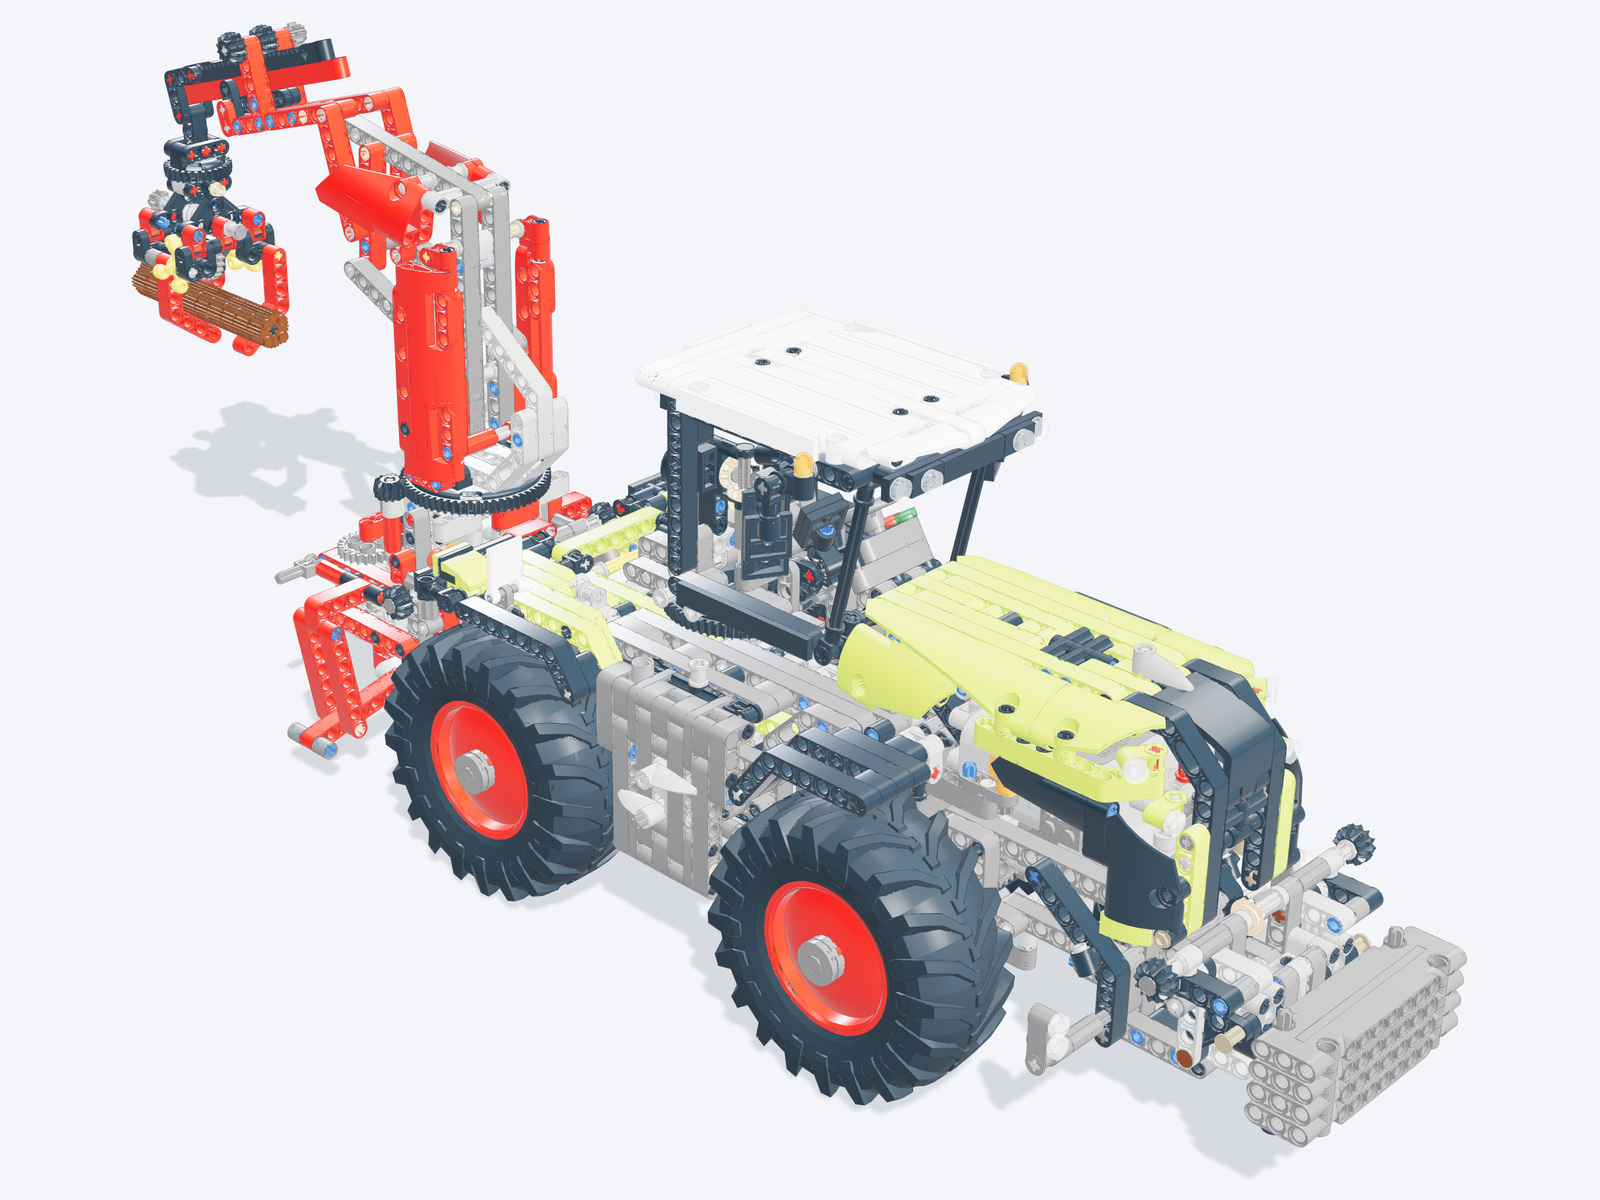
\includegraphics[width=.65\linewidth]{figures-v2/omr-42054-iso.jpg}\end{center}
\paragraph{Attribution.}Philippe Hurbain [Philo]. CC BY 2.0.\par\url{https://library.ldraw.org/library/omr/42054-1.mpd}
\paragraph{Source SHA256.}\path{aa2856b77726aaaa74145ba1e40dbd89d1897ff3577ac2eab83237bd6d65b04c}
\paragraph{Connector records.}stud: 168; axle: 2620; hinge: 2; fixed: 0; ball: 0
\paragraph{Public input lock.}\path{0dec5b93310c7aaf6330dcfaf6e0a0474c1c4f7ad138c1d87013f90de85fa35f}
\paragraph{Status.}Source preservation does not certify stability. Reference outputs below are internal review material. Full model inputs are the versioned public JSON and numbered PNGs.
\begin{enumerate}
\item \textbf{ld2-omr-42054-color-1}. Identify the original color of B1103; numbered isolation is allowed.
\par{\small color; visual; atomic; single-choice.\par\textit{Operands:} B1103 = brick\_001103\par\textit{Public evidence summary:} Numbered PNG: benchmark/ldraw-v2/inputs/views/ld2-omr-42054-color-1.png; structured input = \{\}.\par\textit{Options:} A: Light Bluish Grey; B: Orange; C: Black; D: Rubber Black\par\textit{Reference output:} \{"choiceId": "C"\}\par\textit{Derivation:} source colorName by rendered B-label; source oracle only\par\textit{Equivalence:} exact declared response\par\textit{Review:} pending required human review.}
\item \textbf{ld2-omr-42054-shape-match-1}. Ignoring color and pose, which numbered instance has the same LDraw part type as B1103?
\par{\small shape-match; visual; atomic; single-choice.\par\textit{Operands:} B1536 = brick\_001536, B1103 = brick\_001103, B1754 = brick\_001754, B0911 = brick\_000911, B0158 = brick\_000158\par\textit{Public evidence summary:} Numbered PNG: benchmark/ldraw-v2/inputs/views/ld2-omr-42054-shape-match-1.png; structured input = \{\}.\par\textit{Options:} A: B1754; B: B1536; C: B0911; D: B0158\par\textit{Reference output:} \{"choiceId": "A"\}\par\textit{Derivation:} source partNumber equality across labeled candidates; source oracle only\par\textit{Equivalence:} same source partNumber; ignore color and pose; perceptual equivalence pending\par\textit{Review:} pending required human review.}
\item \textbf{ld2-omr-42054-distance-1}. Using the supplied geometry bounding-box centers, which candidate is nearest to B1103?
\par{\small distance; source-data; atomic; single-choice.\par\textit{Operands:} B0468 = brick\_000468, B1103 = brick\_001103, B1535 = brick\_001535, B0455 = brick\_000455\par\textit{Public evidence summary:} \{"coordinateFrame": "Viewer world, millimeters, Euclidean distance", "centers": \{"B1103": [40, 144, 144], "B1535": [8, 32, -216], "B0468": [-32, 48, 106], "B0455": [-20, 68, 88]\}\}\par\textit{Options:} A: B1535; B: B0468; C: B0455\par\textit{Reference output:} \{"choiceId": "C"\}\par\textit{Derivation:} Euclidean norm from public rounded centers\par\textit{Equivalence:} exact declared response\par\textit{Review:} machine checks passed; no human certification.}
\item \textbf{ld2-omr-42054-color-2}. Identify the original color of B1016; numbered isolation is allowed.
\par{\small color; visual; atomic; single-choice.\par\textit{Operands:} B1016 = brick\_001016\par\textit{Public evidence summary:} Numbered PNG: benchmark/ldraw-v2/inputs/views/ld2-omr-42054-color-2.png; structured input = \{\}.\par\textit{Options:} A: Red; B: Black; C: Orange; D: Pearl Silver\par\textit{Reference output:} \{"choiceId": "B"\}\par\textit{Derivation:} source colorName by rendered B-label; source oracle only\par\textit{Equivalence:} exact declared response\par\textit{Review:} pending required human review.}
\item \textbf{ld2-omr-42054-shape-match-2}. Ignoring color and pose, which numbered instance has the same LDraw part type as B1016?
\par{\small shape-match; visual; atomic; single-choice.\par\textit{Operands:} B0191 = brick\_000191, B0439 = brick\_000439, B1357 = brick\_001357, B1016 = brick\_001016, B1766 = brick\_001766\par\textit{Public evidence summary:} Numbered PNG: benchmark/ldraw-v2/inputs/views/ld2-omr-42054-shape-match-2.png; structured input = \{\}.\par\textit{Options:} A: B1357; B: B0191; C: B1766; D: B0439\par\textit{Reference output:} \{"choiceId": "D"\}\par\textit{Derivation:} source partNumber equality across labeled candidates; source oracle only\par\textit{Equivalence:} same source partNumber; ignore color and pose; perceptual equivalence pending\par\textit{Review:} pending required human review.}
\item \textbf{ld2-omr-42054-distance-2}. Using the supplied geometry bounding-box centers, which candidate is nearest to B1016?
\par{\small distance; source-data; atomic; single-choice.\par\textit{Operands:} B1016 = brick\_001016, B1325 = brick\_001325, B1356 = brick\_001356, B0125 = brick\_000125\par\textit{Public evidence summary:} \{"coordinateFrame": "Viewer world, millimeters, Euclidean distance", "centers": \{"B1016": [8, 120, 72], "B1325": [0, 132, -40], "B1356": [24, 128, -32], "B0125": [0, 88, -104]\}\}\par\textit{Options:} A: B1356; B: B0125; C: B1325\par\textit{Reference output:} \{"choiceId": "A"\}\par\textit{Derivation:} Euclidean norm from public rounded centers\par\textit{Equivalence:} exact declared response\par\textit{Review:} machine checks passed; no human certification.}
\item \textbf{ld2-omr-42054-color-3}. Identify the original color of B0570; numbered isolation is allowed.
\par{\small color; visual; atomic; single-choice.\par\textit{Operands:} B0570 = brick\_000570\par\textit{Public evidence summary:} Numbered PNG: benchmark/ldraw-v2/inputs/views/ld2-omr-42054-color-3.png; structured input = \{\}.\par\textit{Options:} A: Trans Red; B: Rubber Black; C: Trans Orange; D: Dark Bluish Grey\par\textit{Reference output:} \{"choiceId": "D"\}\par\textit{Derivation:} source colorName by rendered B-label; source oracle only\par\textit{Equivalence:} exact declared response\par\textit{Review:} pending required human review.}
\item \textbf{ld2-omr-42054-shape-match-3}. Ignoring color and pose, which numbered instance has the same LDraw part type as B0570?
\par{\small shape-match; visual; atomic; single-choice.\par\textit{Operands:} B1867 = brick\_001867, B0570 = brick\_000570, B1885 = brick\_001885, B0803 = brick\_000803, B1394 = brick\_001394\par\textit{Public evidence summary:} Numbered PNG: benchmark/ldraw-v2/inputs/views/ld2-omr-42054-shape-match-3.png; structured input = \{\}.\par\textit{Options:} A: B1867; B: B1394; C: B0803; D: B1885\par\textit{Reference output:} \{"choiceId": "B"\}\par\textit{Derivation:} source partNumber equality across labeled candidates; source oracle only\par\textit{Equivalence:} same source partNumber; ignore color and pose; perceptual equivalence pending\par\textit{Review:} pending required human review.}
\item \textbf{ld2-omr-42054-distance-3}. Using the supplied geometry bounding-box centers, which candidate is nearest to B0570?
\par{\small distance; source-data; atomic; single-choice.\par\textit{Operands:} B1586 = brick\_001586, B0016 = brick\_000016, B1159 = brick\_001159, B0570 = brick\_000570\par\textit{Public evidence summary:} \{"coordinateFrame": "Viewer world, millimeters, Euclidean distance", "centers": \{"B0570": [16.1, 88, 176], "B1586": [0, 62, -208], "B0016": [0, 96, -24], "B1159": [30.6176, 132.6864, 73.3612]\}\}\par\textit{Options:} A: B1586; B: B1159; C: B0016\par\textit{Reference output:} \{"choiceId": "B"\}\par\textit{Derivation:} Euclidean norm from public rounded centers\par\textit{Equivalence:} exact declared response\par\textit{Review:} pending required human review.}
\item \textbf{ld2-omr-42054-color-4}. Identify the original color of B0724; numbered isolation is allowed.
\par{\small color; visual; atomic; single-choice.\par\textit{Operands:} B0724 = brick\_000724\par\textit{Public evidence summary:} Numbered PNG: benchmark/ldraw-v2/inputs/views/ld2-omr-42054-color-4.png; structured input = \{\}.\par\textit{Options:} A: Pearl Silver; B: White; C: Black; D: Blue\par\textit{Reference output:} \{"choiceId": "C"\}\par\textit{Derivation:} source colorName by rendered B-label; source oracle only\par\textit{Equivalence:} exact declared response\par\textit{Review:} pending required human review.}
\item \textbf{ld2-omr-42054-shape-match-4}. Ignoring color and pose, which numbered instance has the same LDraw part type as B0724?
\par{\small shape-match; visual; atomic; single-choice.\par\textit{Operands:} B0485 = brick\_000485, B0349 = brick\_000349, B1765 = brick\_001765, B0724 = brick\_000724, B0529 = brick\_000529\par\textit{Public evidence summary:} Numbered PNG: benchmark/ldraw-v2/inputs/views/ld2-omr-42054-shape-match-4.png; structured input = \{\}.\par\textit{Options:} A: B1765; B: B0349; C: B0485; D: B0529\par\textit{Reference output:} \{"choiceId": "D"\}\par\textit{Derivation:} source partNumber equality across labeled candidates; source oracle only\par\textit{Equivalence:} same source partNumber; ignore color and pose; perceptual equivalence pending\par\textit{Review:} pending required human review.}
\item \textbf{ld2-omr-42054-distance-4}. Using the supplied geometry bounding-box centers, which candidate is nearest to B0724?
\par{\small distance; source-data; atomic; single-choice.\par\textit{Operands:} B0724 = brick\_000724, B1307 = brick\_001307, B0771 = brick\_000771, B0366 = brick\_000366\par\textit{Public evidence summary:} \{"coordinateFrame": "Viewer world, millimeters, Euclidean distance", "centers": \{"B0724": [-24, 100, 72], "B0771": [-40, 112, -12], "B1307": [-24, 128, -32], "B0366": [0, 86, 8]\}\}\par\textit{Options:} A: B1307; B: B0771; C: B0366\par\textit{Reference output:} \{"choiceId": "C"\}\par\textit{Derivation:} Euclidean norm from public rounded centers\par\textit{Equivalence:} exact declared response\par\textit{Review:} pending required human review.}
\item \textbf{ld2-omr-42054-color-5}. Identify the original color of B1396; numbered isolation is allowed.
\par{\small color; visual; atomic; single-choice.\par\textit{Operands:} B1396 = brick\_001396\par\textit{Public evidence summary:} Numbered PNG: benchmark/ldraw-v2/inputs/views/ld2-omr-42054-color-5.png; structured input = \{\}.\par\textit{Options:} A: Tan; B: Orange; C: Dark Bluish Grey; D: Dark Tan\par\textit{Reference output:} \{"choiceId": "C"\}\par\textit{Derivation:} source colorName by rendered B-label; source oracle only\par\textit{Equivalence:} exact declared response\par\textit{Review:} pending required human review.}
\item \textbf{ld2-omr-42054-shape-match-5}. Ignoring color and pose, which numbered instance has the same LDraw part type as B1396?
\par{\small shape-match; visual; atomic; single-choice.\par\textit{Operands:} B0793 = brick\_000793, B1082 = brick\_001082, B0492 = brick\_000492, B1763 = brick\_001763, B1396 = brick\_001396\par\textit{Public evidence summary:} Numbered PNG: benchmark/ldraw-v2/inputs/views/ld2-omr-42054-shape-match-5.png; structured input = \{\}.\par\textit{Options:} A: B0793; B: B0492; C: B1082; D: B1763\par\textit{Reference output:} \{"choiceId": "C"\}\par\textit{Derivation:} source partNumber equality across labeled candidates; source oracle only\par\textit{Equivalence:} same source partNumber; ignore color and pose; perceptual equivalence pending\par\textit{Review:} pending required human review.}
\item \textbf{ld2-omr-42054-distance-5}. Using the supplied geometry bounding-box centers, which candidate is nearest to B1396?
\par{\small distance; source-data; atomic; single-choice.\par\textit{Operands:} B0365 = brick\_000365, B1396 = brick\_001396, B0049 = brick\_000049, B0827 = brick\_000827\par\textit{Public evidence summary:} \{"coordinateFrame": "Viewer world, millimeters, Euclidean distance", "centers": \{"B1396": [-0.1, 154.0704, 7.7276], "B0365": [0, 74, 8], "B0827": [68, 100, -20], "B0049": [16, 40, -128]\}\}\par\textit{Options:} A: B0827; B: B0049; C: B0365\par\textit{Reference output:} \{"choiceId": "C"\}\par\textit{Derivation:} Euclidean norm from public rounded centers\par\textit{Equivalence:} exact declared response\par\textit{Review:} pending required human review.}
\item \textbf{ld2-omr-42054-interface-1}. Classify the supplied connector record for B1852 and B1848. This does not certify load capacity.
\par{\small interface; connector-graph; metacognitive; single-choice.\par\textit{Operands:} B1848 = brick\_001848, B1852 = brick\_001852\par\textit{Public evidence summary:} \{"connectorRecord": \{"family": "axle", "aConnector": 0, "bConnector": 0\}, "scope": "Upstream connector tolerances and inset mesh intersections; unknown parts remain explicit, separate scene objects are not glued together; no load/force validation."\}\par\textit{Options:} A: stud; B: fixed; C: ball; D: axle; E: hinge\par\textit{Reference output:} \{"choiceId": "D"\}\par\textit{Derivation:} public connectorRecord.family equality\par\textit{Equivalence:} exact declared response\par\textit{Review:} machine checks passed; no human certification.}
\item \textbf{ld2-omr-42054-interface-2}. Classify the supplied connector record for B1825 and B1824. This does not certify load capacity.
\par{\small interface; connector-graph; metacognitive; single-choice.\par\textit{Operands:} B1824 = brick\_001824, B1825 = brick\_001825\par\textit{Public evidence summary:} \{"connectorRecord": \{"family": "hinge", "aConnector": 1, "bConnector": 1\}, "scope": "Upstream connector tolerances and inset mesh intersections; unknown parts remain explicit, separate scene objects are not glued together; no load/force validation."\}\par\textit{Options:} A: ball; B: hinge; C: fixed; D: axle; E: stud\par\textit{Reference output:} \{"choiceId": "B"\}\par\textit{Derivation:} public connectorRecord.family equality\par\textit{Equivalence:} exact declared response\par\textit{Review:} machine checks passed; no human certification.}
\item \textbf{ld2-omr-42054-interface-3}. Classify the supplied connector record for B0940 and B0942. This does not certify load capacity.
\par{\small interface; connector-graph; metacognitive; single-choice.\par\textit{Operands:} B0942 = brick\_000942, B0940 = brick\_000940\par\textit{Public evidence summary:} \{"connectorRecord": \{"family": "stud", "aConnector": 5, "bConnector": 0\}, "scope": "Upstream connector tolerances and inset mesh intersections; unknown parts remain explicit, separate scene objects are not glued together; no load/force validation."\}\par\textit{Options:} A: stud; B: hinge; C: ball; D: fixed; E: axle\par\textit{Reference output:} \{"choiceId": "A"\}\par\textit{Derivation:} public connectorRecord.family equality\par\textit{Equivalence:} exact declared response\par\textit{Review:} machine checks passed; no human certification.}
\item \textbf{ld2-omr-42054-neighbors-1}. Select every candidate directly adjacent to B1563 in the supplied connector graph.
\par{\small neighbors; connector-graph; metacognitive; multiple-choice.\par\textit{Operands:} B1563 = brick\_001563, B1037 = brick\_001037, B0192 = brick\_000192, B1559 = brick\_001559, B1565 = brick\_001565\par\textit{Public evidence summary:} 2 unique undirected pairs\par\textit{Options:} A: B1565; B: B0192; C: B1559; D: B1037\par\textit{Reference output:} \{"choiceIds": ["A", "C"]\}\par\textit{Derivation:} public incident edge endpoint set\par\textit{Equivalence:} unordered exact set; duplicate IDs invalid\par\textit{Review:} machine checks passed; no human certification.}
\item \textbf{ld2-omr-42054-graph-removal-1}. Delete B1563 and its incident edges from this local graph. How many connected components remain? Do not infer physical extractability.
\par{\small graph-removal; connector-graph; graph-internal; integer.\par\textit{Operands:} B1559 = brick\_001559, B1565 = brick\_001565, B1037 = brick\_001037, B0192 = brick\_000192, B1563 = brick\_001563\par\textit{Public evidence summary:} 2 unique undirected pairs; 5 nodes\par\textit{Reference output:} \{"value": 4\}\par\textit{Derivation:} union-find component count after public target deletion\par\textit{Equivalence:} exact declared response\par\textit{Review:} machine checks passed; no human certification.}
\item \textbf{ld2-omr-42054-neighbors-2}. Select every candidate directly adjacent to B0710 in the supplied connector graph.
\par{\small neighbors; connector-graph; metacognitive; multiple-choice.\par\textit{Operands:} B0711 = brick\_000711, B1619 = brick\_001619, B0644 = brick\_000644, B0710 = brick\_000710, B1207 = brick\_001207\par\textit{Public evidence summary:} 2 unique undirected pairs\par\textit{Options:} A: B0711; B: B0644; C: B1207; D: B1619\par\textit{Reference output:} \{"choiceIds": ["A", "B"]\}\par\textit{Derivation:} public incident edge endpoint set\par\textit{Equivalence:} unordered exact set; duplicate IDs invalid\par\textit{Review:} machine checks passed; no human certification.}
\item \textbf{ld2-omr-42054-graph-removal-2}. Delete B0710 and its incident edges from this local graph. How many connected components remain? Do not infer physical extractability.
\par{\small graph-removal; connector-graph; graph-internal; integer.\par\textit{Operands:} B1619 = brick\_001619, B0711 = brick\_000711, B0710 = brick\_000710, B1207 = brick\_001207, B0644 = brick\_000644\par\textit{Public evidence summary:} 2 unique undirected pairs; 5 nodes\par\textit{Reference output:} \{"value": 4\}\par\textit{Derivation:} union-find component count after public target deletion\par\textit{Equivalence:} exact declared response\par\textit{Review:} machine checks passed; no human certification.}
\item \textbf{ld2-omr-42054-neighbors-3}. Select every candidate directly adjacent to B1218 in the supplied connector graph.
\par{\small neighbors; connector-graph; metacognitive; multiple-choice.\par\textit{Operands:} B0876 = brick\_000876, B0027 = brick\_000027, B1218 = brick\_001218, B1217 = brick\_001217, B1219 = brick\_001219, B1216 = brick\_001216\par\textit{Public evidence summary:} 3 unique undirected pairs\par\textit{Options:} A: B0876; B: B1216; C: B1217; D: B0027; E: B1219\par\textit{Reference output:} \{"choiceIds": ["B", "C", "E"]\}\par\textit{Derivation:} public incident edge endpoint set\par\textit{Equivalence:} unordered exact set; duplicate IDs invalid\par\textit{Review:} machine checks passed; no human certification.}
\item \textbf{ld2-omr-42054-graph-removal-3}. Delete B1218 and its incident edges from this local graph. How many connected components remain? Do not infer physical extractability.
\par{\small graph-removal; connector-graph; graph-internal; integer.\par\textit{Operands:} B0027 = brick\_000027, B1219 = brick\_001219, B0876 = brick\_000876, B1216 = brick\_001216, B1217 = brick\_001217, B1218 = brick\_001218\par\textit{Public evidence summary:} 3 unique undirected pairs; 6 nodes\par\textit{Reference output:} \{"value": 5\}\par\textit{Derivation:} union-find component count after public target deletion\par\textit{Equivalence:} exact declared response\par\textit{Review:} machine checks passed; no human certification.}
\item \textbf{ld2-omr-42054-neighbors-4}. Select every candidate directly adjacent to B0478 in the supplied connector graph.
\par{\small neighbors; connector-graph; metacognitive; multiple-choice.\par\textit{Operands:} B0505 = brick\_000505, B0459 = brick\_000459, B0463 = brick\_000463, B1616 = brick\_001616, B0462 = brick\_000462, B0468 = brick\_000468, B0469 = brick\_000469, B0125 = brick\_000125, B0478 = brick\_000478\par\textit{Public evidence summary:} 6 unique undirected pairs\par\textit{Options:} A: B0468; B: B0469; C: B0505; D: B0459; E: B0462; F: B0125; G: B0463; H: B1616\par\textit{Reference output:} \{"choiceIds": ["A", "B", "C", "D", "E", "G"]\}\par\textit{Derivation:} public incident edge endpoint set\par\textit{Equivalence:} unordered exact set; duplicate IDs invalid\par\textit{Review:} machine checks passed; no human certification.}
\item \textbf{ld2-omr-42054-graph-removal-4}. Delete B0478 and its incident edges from this local graph. How many connected components remain? Do not infer physical extractability.
\par{\small graph-removal; connector-graph; graph-internal; integer.\par\textit{Operands:} B0478 = brick\_000478, B0469 = brick\_000469, B0459 = brick\_000459, B1616 = brick\_001616, B0462 = brick\_000462, B0125 = brick\_000125, B0505 = brick\_000505, B0468 = brick\_000468, B0463 = brick\_000463\par\textit{Public evidence summary:} 6 unique undirected pairs; 9 nodes\par\textit{Reference output:} \{"value": 8\}\par\textit{Derivation:} union-find component count after public target deletion\par\textit{Equivalence:} exact declared response\par\textit{Review:} machine checks passed; no human certification.}
\item \textbf{ld2-omr-42054-neighbors-5}. Select every candidate directly adjacent to B1973 in the supplied connector graph.
\par{\small neighbors; connector-graph; metacognitive; multiple-choice.\par\textit{Operands:} B1973 = brick\_001973, B1967 = brick\_001967, B0748 = brick\_000748, B1547 = brick\_001547, B1972 = brick\_001972, B1974 = brick\_001974\par\textit{Public evidence summary:} 5 unique undirected pairs\par\textit{Options:} A: B1967; B: B1547; C: B1974; D: B1972; E: B0748\par\textit{Reference output:} \{"choiceIds": ["A", "C", "D"]\}\par\textit{Derivation:} public incident edge endpoint set\par\textit{Equivalence:} unordered exact set; duplicate IDs invalid\par\textit{Review:} machine checks passed; no human certification.}
\item \textbf{ld2-omr-42054-graph-removal-5}. Delete B1973 and its incident edges from this local graph. How many connected components remain? Do not infer physical extractability.
\par{\small graph-removal; connector-graph; graph-internal; integer.\par\textit{Operands:} B1547 = brick\_001547, B1973 = brick\_001973, B1974 = brick\_001974, B1967 = brick\_001967, B1972 = brick\_001972, B0748 = brick\_000748\par\textit{Public evidence summary:} 5 unique undirected pairs; 6 nodes\par\textit{Reference output:} \{"value": 3\}\par\textit{Derivation:} union-find component count after public target deletion\par\textit{Equivalence:} exact declared response\par\textit{Review:} machine checks passed; no human certification.}
\item \textbf{ld2-omr-42054-coverage-1}. Which numbered instance lacks a connector definition in the coverage record, so this audit cannot establish that it is floating?
\par{\small coverage; source-data; metacognitive; single-choice.\par\textit{Operands:} B1016 = brick\_001016, B0570 = brick\_000570, B1103 = brick\_001103, B0146 = brick\_000146\par\textit{Public evidence summary:} \{"coverage": [\{"label": "B0146", "supported": false\}, \{"label": "B0570", "supported": true\}, \{"label": "B1103", "supported": true\}, \{"label": "B1016", "supported": true\}]\}\par\textit{Options:} A: B0570; B: B0146; C: B1103; D: B1016\par\textit{Reference output:} \{"choiceId": "B"\}\par\textit{Derivation:} public supported=false record\par\textit{Equivalence:} exact declared response\par\textit{Review:} pending required human review.}
\item \textbf{ld2-omr-42054-evidence-limit-1}. Only source geometry, connector matching and mesh intersection audits are available. Without mass, friction, material or dynamic tests, is gravitational stability established?
\par{\small evidence-limit; source-data; metacognitive; single-choice.\par\textit{Operands:} none\par\textit{Public evidence summary:} \{"available": ["Original CAD", "Connector inference", "Inset-mesh intersection candidates"]\}\par\textit{Options:} A: Not established by this evidence; B: Established\par\textit{Reference output:} \{"choiceId": "A"\}\par\textit{Derivation:} fixed epistemic control label\par\textit{Equivalence:} exact declared response\par\textit{Review:} machine checks passed; no human certification.}
\item \textbf{ld2-omr-42054-source-step-1}. At which expanded author step does B1230 first appear in the supplied source-step table? Source order is not a collision-free assembly proof.
\par{\small source-step; source-data; procedural; single-choice.\par\textit{Operands:} B0001 = brick\_000001, B1230 = brick\_001230\par\textit{Public evidence summary:} 2 supplied author-step records; exact table in public JSON\par\textit{Options:} A: 48; B: 95; C: 135; D: 109\par\textit{Reference output:} \{"choiceId": "C"\}\par\textit{Derivation:} minimum public step index containing target\par\textit{Equivalence:} exact declared response\par\textit{Review:} machine checks passed; no human certification.}
\item \textbf{ld2-omr-42054-source-step-2}. At which expanded author step does B1177 first appear in the supplied source-step table? Source order is not a collision-free assembly proof.
\par{\small source-step; source-data; procedural; single-choice.\par\textit{Operands:} B1177 = brick\_001177, B0001 = brick\_000001\par\textit{Public evidence summary:} 2 supplied author-step records; exact table in public JSON\par\textit{Options:} A: 131; B: 221; C: 132; D: 206\par\textit{Reference output:} \{"choiceId": "A"\}\par\textit{Derivation:} minimum public step index containing target\par\textit{Equivalence:} exact declared response\par\textit{Review:} machine checks passed; no human certification.}
\item \textbf{ld2-omr-42054-source-step-3}. At which expanded author step does B0711 first appear in the supplied source-step table? Source order is not a collision-free assembly proof.
\par{\small source-step; source-data; procedural; single-choice.\par\textit{Operands:} B0711 = brick\_000711, B0001 = brick\_000001\par\textit{Public evidence summary:} 2 supplied author-step records; exact table in public JSON\par\textit{Options:} A: 65; B: 175; C: 85; D: 136\par\textit{Reference output:} \{"choiceId": "C"\}\par\textit{Derivation:} minimum public step index containing target\par\textit{Equivalence:} exact declared response\par\textit{Review:} machine checks passed; no human certification.}
\item \textbf{ld2-omr-42054-source-step-4}. At which expanded author step does B0180 first appear in the supplied source-step table? Source order is not a collision-free assembly proof.
\par{\small source-step; source-data; procedural; single-choice.\par\textit{Operands:} B0001 = brick\_000001, B0180 = brick\_000180\par\textit{Public evidence summary:} 2 supplied author-step records; exact table in public JSON\par\textit{Options:} A: 136; B: 30; C: 19; D: 82\par\textit{Reference output:} \{"choiceId": "C"\}\par\textit{Derivation:} minimum public step index containing target\par\textit{Equivalence:} exact declared response\par\textit{Review:} machine checks passed; no human certification.}
\item \textbf{ld2-omr-42054-source-step-5}. At which expanded author step does B0363 first appear in the supplied source-step table? Source order is not a collision-free assembly proof.
\par{\small source-step; source-data; procedural; single-choice.\par\textit{Operands:} B0001 = brick\_000001, B0363 = brick\_000363\par\textit{Public evidence summary:} 2 supplied author-step records; exact table in public JSON\par\textit{Options:} A: 128; B: 19; C: 43; D: 11\par\textit{Reference output:} \{"choiceId": "C"\}\par\textit{Derivation:} minimum public step index containing target\par\textit{Equivalence:} exact declared response\par\textit{Review:} machine checks passed; no human certification.}
\item \textbf{ld2-omr-42054-source-sequence-1}. Reveal the supplied source-step window in author order. Actions change visibility only, without simulating insertion trajectories.
\par{\small source-sequence; scene-edit; procedural; actions.\par\textit{Operands:} B0027 = brick\_000027, B0021 = brick\_000021, B0047 = brick\_000047, B0044 = brick\_000044, B0001 = brick\_000001, B0035 = brick\_000035, B0025 = brick\_000025, B0042 = brick\_000042, B0005 = brick\_000005, B0020 = brick\_000020, B0058 = brick\_000058, B0050 = brick\_000050, B0037 = brick\_000037, B0003 = brick\_000003, B0039 = brick\_000039, B0030 = brick\_000030, B0029 = brick\_000029, B0034 = brick\_000034, B0009 = brick\_000009, B0011 = brick\_000011, B0016 = brick\_000016, B0012 = brick\_000012, B0051 = brick\_000051, B0022 = brick\_000022, B0004 = brick\_000004, B0048 = brick\_000048, B0006 = brick\_000006, B0046 = brick\_000046, B0023 = brick\_000023, B0032 = brick\_000032, B0013 = brick\_000013, B0019 = brick\_000019, B0026 = brick\_000026, B0014 = brick\_000014, B0031 = brick\_000031, B0024 = brick\_000024, B0056 = brick\_000056, B0017 = brick\_000017, B0008 = brick\_000008, B0007 = brick\_000007, B0045 = brick\_000045, B0053 = brick\_000053, B0018 = brick\_000018, B0041 = brick\_000041, B0038 = brick\_000038, B0036 = brick\_000036, B0057 = brick\_000057, B0010 = brick\_000010, B0043 = brick\_000043, B0052 = brick\_000052, B0054 = brick\_000054, B0033 = brick\_000033, B0055 = brick\_000055, B0028 = brick\_000028, B0002 = brick\_000002, B0049 = brick\_000049, B0040 = brick\_000040, B0015 = brick\_000015\par\textit{Public evidence summary:} 6 public actions; budget 6; \{"initialFacts": ["start"], "goalFacts": ["done-6"], "absentFacts": []\}\par\textit{Reference output:} \{"actionIds": ["step-1", "step-2", "step-3", "step-4", "step-5", "step-6"]\}\par\textit{Derivation:} public precondition solver\par\textit{Equivalence:} any legal sequence reaching all goals within budget; display-only semantics\par\textit{Review:} pending required human review.}
\item \textbf{ld2-omr-42054-restore-instance-1}. The display copy hides B1103. Restore only that numbered instance, preserving all other instances and source poses.
\par{\small restore-instance; scene-edit; procedural; actions.\par\textit{Operands:} B1103 = brick\_001103, B0001 = brick\_000001\par\textit{Public evidence summary:} 2 public actions; budget 1; \{"initialFacts": ["missing-brick\_001103", "present-brick\_000001"], "goalFacts": ["present-brick\_001103", "present-brick\_000001"], "absentFacts": ["missing-brick\_001103"]\}\par\textit{Reference output:} \{"actionIds": ["restore-B1103"]\}\par\textit{Derivation:} public precondition solver\par\textit{Equivalence:} any legal sequence reaching all goals within budget; display-only semantics\par\textit{Review:} machine checks passed; no human certification.}
\item \textbf{ld2-omr-42054-restore-instance-2}. The display copy hides B1016. Restore only that numbered instance, preserving all other instances and source poses.
\par{\small restore-instance; scene-edit; procedural; actions.\par\textit{Operands:} B0001 = brick\_000001, B1016 = brick\_001016\par\textit{Public evidence summary:} 2 public actions; budget 1; \{"initialFacts": ["missing-brick\_001016", "present-brick\_000001"], "goalFacts": ["present-brick\_001016", "present-brick\_000001"], "absentFacts": ["missing-brick\_001016"]\}\par\textit{Reference output:} \{"actionIds": ["restore-B1016"]\}\par\textit{Derivation:} public precondition solver\par\textit{Equivalence:} any legal sequence reaching all goals within budget; display-only semantics\par\textit{Review:} machine checks passed; no human certification.}
\item \textbf{ld2-omr-42054-restore-instance-3}. The display copy hides B0570. Restore only that numbered instance, preserving all other instances and source poses.
\par{\small restore-instance; scene-edit; procedural; actions.\par\textit{Operands:} B0570 = brick\_000570, B0001 = brick\_000001\par\textit{Public evidence summary:} 2 public actions; budget 1; \{"initialFacts": ["missing-brick\_000570", "present-brick\_000001"], "goalFacts": ["present-brick\_000570", "present-brick\_000001"], "absentFacts": ["missing-brick\_000570"]\}\par\textit{Reference output:} \{"actionIds": ["restore-B0570"]\}\par\textit{Derivation:} public precondition solver\par\textit{Equivalence:} any legal sequence reaching all goals within budget; display-only semantics\par\textit{Review:} machine checks passed; no human certification.}
\end{enumerate}

\end{document}
